\documentclass[]{book}
\usepackage{lmodern}
\usepackage{amssymb,amsmath}
\usepackage{ifxetex,ifluatex}
\usepackage{fixltx2e} % provides \textsubscript
\ifnum 0\ifxetex 1\fi\ifluatex 1\fi=0 % if pdftex
  \usepackage[T1]{fontenc}
  \usepackage[utf8]{inputenc}
\else % if luatex or xelatex
  \ifxetex
    \usepackage{mathspec}
  \else
    \usepackage{fontspec}
  \fi
  \defaultfontfeatures{Ligatures=TeX,Scale=MatchLowercase}
\fi
% use upquote if available, for straight quotes in verbatim environments
\IfFileExists{upquote.sty}{\usepackage{upquote}}{}
% use microtype if available
\IfFileExists{microtype.sty}{%
\usepackage{microtype}
\UseMicrotypeSet[protrusion]{basicmath} % disable protrusion for tt fonts
}{}
\usepackage{hyperref}
\hypersetup{unicode=true,
            pdftitle={R, Not the Best Practices},
            pdfauthor={Nikita Voevodin},
            pdfborder={0 0 0},
            breaklinks=true}
\urlstyle{same}  % don't use monospace font for urls
\usepackage{natbib}
\bibliographystyle{apalike}
\usepackage{color}
\usepackage{fancyvrb}
\newcommand{\VerbBar}{|}
\newcommand{\VERB}{\Verb[commandchars=\\\{\}]}
\DefineVerbatimEnvironment{Highlighting}{Verbatim}{commandchars=\\\{\}}
% Add ',fontsize=\small' for more characters per line
\usepackage{framed}
\definecolor{shadecolor}{RGB}{248,248,248}
\newenvironment{Shaded}{\begin{snugshade}}{\end{snugshade}}
\newcommand{\AlertTok}[1]{\textcolor[rgb]{0.94,0.16,0.16}{#1}}
\newcommand{\AnnotationTok}[1]{\textcolor[rgb]{0.56,0.35,0.01}{\textbf{\textit{#1}}}}
\newcommand{\AttributeTok}[1]{\textcolor[rgb]{0.77,0.63,0.00}{#1}}
\newcommand{\BaseNTok}[1]{\textcolor[rgb]{0.00,0.00,0.81}{#1}}
\newcommand{\BuiltInTok}[1]{#1}
\newcommand{\CharTok}[1]{\textcolor[rgb]{0.31,0.60,0.02}{#1}}
\newcommand{\CommentTok}[1]{\textcolor[rgb]{0.56,0.35,0.01}{\textit{#1}}}
\newcommand{\CommentVarTok}[1]{\textcolor[rgb]{0.56,0.35,0.01}{\textbf{\textit{#1}}}}
\newcommand{\ConstantTok}[1]{\textcolor[rgb]{0.00,0.00,0.00}{#1}}
\newcommand{\ControlFlowTok}[1]{\textcolor[rgb]{0.13,0.29,0.53}{\textbf{#1}}}
\newcommand{\DataTypeTok}[1]{\textcolor[rgb]{0.13,0.29,0.53}{#1}}
\newcommand{\DecValTok}[1]{\textcolor[rgb]{0.00,0.00,0.81}{#1}}
\newcommand{\DocumentationTok}[1]{\textcolor[rgb]{0.56,0.35,0.01}{\textbf{\textit{#1}}}}
\newcommand{\ErrorTok}[1]{\textcolor[rgb]{0.64,0.00,0.00}{\textbf{#1}}}
\newcommand{\ExtensionTok}[1]{#1}
\newcommand{\FloatTok}[1]{\textcolor[rgb]{0.00,0.00,0.81}{#1}}
\newcommand{\FunctionTok}[1]{\textcolor[rgb]{0.00,0.00,0.00}{#1}}
\newcommand{\ImportTok}[1]{#1}
\newcommand{\InformationTok}[1]{\textcolor[rgb]{0.56,0.35,0.01}{\textbf{\textit{#1}}}}
\newcommand{\KeywordTok}[1]{\textcolor[rgb]{0.13,0.29,0.53}{\textbf{#1}}}
\newcommand{\NormalTok}[1]{#1}
\newcommand{\OperatorTok}[1]{\textcolor[rgb]{0.81,0.36,0.00}{\textbf{#1}}}
\newcommand{\OtherTok}[1]{\textcolor[rgb]{0.56,0.35,0.01}{#1}}
\newcommand{\PreprocessorTok}[1]{\textcolor[rgb]{0.56,0.35,0.01}{\textit{#1}}}
\newcommand{\RegionMarkerTok}[1]{#1}
\newcommand{\SpecialCharTok}[1]{\textcolor[rgb]{0.00,0.00,0.00}{#1}}
\newcommand{\SpecialStringTok}[1]{\textcolor[rgb]{0.31,0.60,0.02}{#1}}
\newcommand{\StringTok}[1]{\textcolor[rgb]{0.31,0.60,0.02}{#1}}
\newcommand{\VariableTok}[1]{\textcolor[rgb]{0.00,0.00,0.00}{#1}}
\newcommand{\VerbatimStringTok}[1]{\textcolor[rgb]{0.31,0.60,0.02}{#1}}
\newcommand{\WarningTok}[1]{\textcolor[rgb]{0.56,0.35,0.01}{\textbf{\textit{#1}}}}
\usepackage{longtable,booktabs}
\usepackage{graphicx,grffile}
\makeatletter
\def\maxwidth{\ifdim\Gin@nat@width>\linewidth\linewidth\else\Gin@nat@width\fi}
\def\maxheight{\ifdim\Gin@nat@height>\textheight\textheight\else\Gin@nat@height\fi}
\makeatother
% Scale images if necessary, so that they will not overflow the page
% margins by default, and it is still possible to overwrite the defaults
% using explicit options in \includegraphics[width, height, ...]{}
\setkeys{Gin}{width=\maxwidth,height=\maxheight,keepaspectratio}
\IfFileExists{parskip.sty}{%
\usepackage{parskip}
}{% else
\setlength{\parindent}{0pt}
\setlength{\parskip}{6pt plus 2pt minus 1pt}
}
\setlength{\emergencystretch}{3em}  % prevent overfull lines
\providecommand{\tightlist}{%
  \setlength{\itemsep}{0pt}\setlength{\parskip}{0pt}}
\setcounter{secnumdepth}{5}
% Redefines (sub)paragraphs to behave more like sections
\ifx\paragraph\undefined\else
\let\oldparagraph\paragraph
\renewcommand{\paragraph}[1]{\oldparagraph{#1}\mbox{}}
\fi
\ifx\subparagraph\undefined\else
\let\oldsubparagraph\subparagraph
\renewcommand{\subparagraph}[1]{\oldsubparagraph{#1}\mbox{}}
\fi

%%% Use protect on footnotes to avoid problems with footnotes in titles
\let\rmarkdownfootnote\footnote%
\def\footnote{\protect\rmarkdownfootnote}

%%% Change title format to be more compact
\usepackage{titling}

% Create subtitle command for use in maketitle
\providecommand{\subtitle}[1]{
  \posttitle{
    \begin{center}\large#1\end{center}
    }
}

\setlength{\droptitle}{-2em}

  \title{R, Not the Best Practices}
    \pretitle{\vspace{\droptitle}\centering\huge}
  \posttitle{\par}
    \author{Nikita Voevodin}
    \preauthor{\centering\large\emph}
  \postauthor{\par}
      \predate{\centering\large\emph}
  \postdate{\par}
    \date{2020-02-09}

\usepackage{booktabs}
\usepackage{amsthm}
\makeatletter
\def\thm@space@setup{%
  \thm@preskip=8pt plus 2pt minus 4pt
  \thm@postskip=\thm@preskip
}
\makeatother

\begin{document}
\maketitle

{
\setcounter{tocdepth}{1}
\tableofcontents
}
\hypertarget{credits}{%
\chapter{Credits}\label{credits}}

Special credits go to Fausto Lopez for his contributions to this book. Fausto was responsible for proofreading as well as the following:

\begin{itemize}
\tightlist
\item
  Popup task 1 (blabla)
\item
  Popup task 2 (blabla)
\item
  Chapter on Stackowerflow
\item
  \ldots{}
\end{itemize}

Currently, Fausto is a Director of Data Analytics at NYC Taxi and Limousine Commission \ldots{}

Special thanks go to the Taxi and Limousine Commission of NYC for providing foundation for my learning process and overall professional developement. blabla.

\hypertarget{intro}{%
\chapter{Intro}\label{intro}}


\includegraphics[width=0.65\linewidth,style="float:right; padding:10px"]{R}

Welcome to ``R, Not the Best Practices''. If you selected this book for one of the following three reasons. One, you saw the title and the cover and though that it was intersting and funny for the guide type of book to be called `Not the Best Practices' and were curious to see what is inside. Two, you know that books that are called `something something, best practices' are hard to follow, because they are written be a person who already forgot how it feels to not know stuff and, therefore, describes things in a manner that is hard to follow. Third, someone referred you to this book, because they learned a lot from it themselves. I am hoping that your reason is somewhere between the second and third points. Although, even if it is the first, you will not regret it.

Why is this book called `Not the Best Practices'? Simple, you do not learn by looking at the perfect code. If I wrote a vectorized loop with a custom function and told you that this is the most efficient way of doing whatever I am doing, therefore, the best practice, you would never understand what the fuck was going on and would just switch off right there and then. That was my experience with the majority of tutorials that I went through. Every time, at some point, I would just stop getting what was going on. But because I had invested some time and money into them I would force myself through them regardless. Unfortunatelly, that tactic results in very little progress and a lot of discouragement. Writing this book, I want it to be nothing like those experiences. There will be some boring basic shit that I just muыt cover, but the majority of it will be practice and interaction driven.

\hypertarget{what-this-book-is-and-is-not}{%
\section{What this book is and is not}\label{what-this-book-is-and-is-not}}

\begin{itemize}
\tightlist
\item
  This book is not written by an academic.
\end{itemize}

I am not an R professor or creator of some fancy library. I am a professional data analyst and an R, SQL and Javascript practitioner.

\begin{itemize}
\tightlist
\item
  This book is not a set of best practices.
\end{itemize}

I do not care about the clengliness of your code, especially at this stage of your progress. The only thing that I care about is whether your code does the job. The best practices will come later. This book is a set of tips, tricks, hacks, and practices (good or bad) that will make things work for you when you need them to.

\begin{itemize}
\tightlist
\item
  This book will not filter words.
\end{itemize}

It is my belief that learning to code can be dull, boring, and discouraging. Therefore, I will to maintain your interest by using some seasoned language here and there. So, if you are extra sensitive, this one might not be for you. In fact, there is a `Vanilla' version of this book available. Ultimatelly, this book will show you how learning R and its components can be frustrating and will give you anecdotal tips on how to go about the grind.

\begin{itemize}
\tightlist
\item
  This book will not use stupid generic data.
\end{itemize}

I have seen and practiced with with a bunch of stupic and semi generic data that makes no fucking sence. That really traumatized me and I do not want you to experience the same pain. Not only we will be working with real data (real vehicles vin numbers, and NYPD car crash data across NYC), but also, we will be pulling that data from the real SQL database that I specifically set up for this book. So, you can be sure that we will not be writing stupid `hello world' examples on every turn. By the end of this book you will have something interesting to show for the time that you invested.

\begin{itemize}
\tightlist
\item
  This book is not only about R.
\end{itemize}

In a professional setup, R goes hand in hand with another language that is extreamly important. This language is SQL, the language of database interaction. To get our practice data, we will be using SQL database table and the SQL language to write commands. On top of that, I will also explaing a good deal about other programming languages and how they interact of dont with R.

\begin{itemize}
\tightlist
\item
  Finally, this book is not only for you.
\end{itemize}

You see, when coding, after a while, you will begin to forget what you've learned or how you've built things. This book therefore, will serve me as a reminder or documentation of things that I have done and built, and as a side effect it will teach you those things as well.

\hypertarget{what-will-this-book-teach-you}{%
\section{What will this book teach you}\label{what-will-this-book-teach-you}}

This book will follow my first three months of learning R at my new job. Before that point, I was ok with computers for playing games and using Microsoft Work and Excel for professional stuff. However, I did not know anything about programming, I did not know any programmers. Code for me was just that, a code. Since the memories of not knowing shit are still fresh in me, I feel quite confident that I should be able to put myself in your shoes and bring you to the level of proficiency the you should be at after learning R for three months. Yes, three months. This book will cover my first quarter of dealing with R and programming in general. If you are already thinking, `Oh shit, this guy will only show me some basic stuff!', you are wrong. I will have to show you some basic stuff, there is no way around it if you want to learn. However, the most of the book will be taken by the real life examples, things that you will be dealing with ninty five percent of a time. For instance, the core of this book revolves around the main assignment that I received in the second week of my employment. That assignment took me offguard and took me two months of non-stop learning of R and SQL to complete. By the end of that assignment I felt comfortable with the most tasks where I needed to work with data. I will lead you through the same experience with many tips and tricks along the way. You will learn how to interact with databases in R; pull data; aggregate and reshape it to your liking; merge it with other data; save it; work with different data and time formats; create useful static and dynamic plots; fit all that nice stuff into presentable reports; create shitty and great maps; use all that again to create dashboards; and finally build a simple web app as a bonus. Along the way, I will be telling you about mine and other programmer's experinces with some peripheral programming topics. If all that is not enough for you, feel free to close this book and get yourself something like `R for Dummies' or some shit. This book is, ultimatelly, what and how I wanted to be taught when I was a noob.

\hypertarget{languages-infrastructure-and-myself}{%
\chapter{Languages, Infrastructure, and Myself}\label{languages-infrastructure-and-myself}}

\hypertarget{about-programming-languages-and-r-place-among-them}{%
\section{About programming languages and R' place among them}\label{about-programming-languages-and-r-place-among-them}}

\hypertarget{r}{%
\subsection{R}\label{r}}

If you are new to programming and if you are reading this book you probably are, or if you are reading this to learn how to create some cool web apps using R Shiny, then explaining to you that R is a functional language and Java is an object oriented language will not make any sense to you or just will not be useful. Instead, I just want to write a few words here about how I see the R universe and how it touches or, does not, other languages. I will definitely not cover all the languages, not even close, and I might not even be hundred percent accurate all the time. However, I will cover everything that I think you will need to start with R and to get to a decent level. The goal here is to make sure you have an overall understanding of the environment you will be working in. I want to make sure that you retain as much information as possible, therefore I will not be stuffing you brain with information you do not need at the moment or will not need any time soon. Once you feel comfortable with your level, obviously, go ahead and learn some advanced geek stuff about different languages and who and how and why built them.

First of all, R is an open-source (free) programming language that focuses on working with data, statistical computation, and graphical visualization. It is widely used by academics, statisticians, data miners, and big data companies to work with all sorts of information. Just to give you a perspective of how popular it is in its field, here is a list of 10 largest R users:

\begin{itemize}
\item
  Facebook
\item
  Google
\item
  Twitter
\item
  Microsoft
\item
  Uber
\item
  Airbnb
\item
  IBM
\item
  HP
\item
  Ford
\item
  New York Times

  Some of these might not exist when you are reading this (UBER lol). These companies use R for things like behavior analysis, data forecasting, various advanced visualizations and statistical modeling. We will not be doing those things but it is good to know that the language that you are using is popular with some big names.

  Secondly, R is different from most other languages because of how it works with data. That is its main advantage and appeal. The way I see it is represented in the following diagram:
\end{itemize}

\hypertarget{excel}{%
\subsection{Excel}\label{excel}}

You are probably familiar with Excel and know what an excel table looks like. When you will start working with R you will notice that you are also working with tables most of the time. Just like in excel. Well, you will probably think that tables like that are supported by every language, for example JavaScript, Java, PHP and other big ones. You would be wrong. These languages do not work with data like Excel or R. Simple operations like joining two tables and aggregating them somehow, that would take two or three lines of code in R, will require some substantial coding and time in those languages, especially if you are new. But how DO those languages work with data? It is definitely possible, however, they are just not made for that. Most of the time, these languages connect to SQL database and use SQL language to work with tabular data. You do not need to worry about that right now. All you need to remember is that R is designed to work with data and you will be much more efficient using R compared to the languages mentioned above. But what about these other languages in the diagram? Well, we have already covered Excel.

\hypertarget{stata-spss-and-sas}{%
\subsection{STATA, SPSS, and SAS}\label{stata-spss-and-sas}}

STATA, SPSS, and SAS are powerful but outdated and expensive statistical packages that also work with tabular data just like excel and R. They are not programming languages and unless you want to find yourself hungry crawling on the floor looking for rats to eat in your studio that you share with some unemployed actor, because nobody wants that shit, I would recommend to stay away from them.

\hypertarget{python}{%
\subsection{Python}\label{python}}

Finally, Python is a full fledged general purpose programming language. It is very hot right now and it seems like every homeless guy knows it already. That, plus the fact that Python is not specifically built to work with data makes me think that a combination of R with something like JavaScript makes more sense. Dont get me wrong, Python is a great and powerful language and is really dominating R at the moment. I used both and found R easier to set up and start working. To put it simply, Python tries to mimic what R does natively by creating additional packages that are just not as powerful. Pythonistas might dispute that but if you are reading this, I im assuming that you have made you choice at least for the moment and im just trying to confirm that you were right.

\begin{figure}
\centering
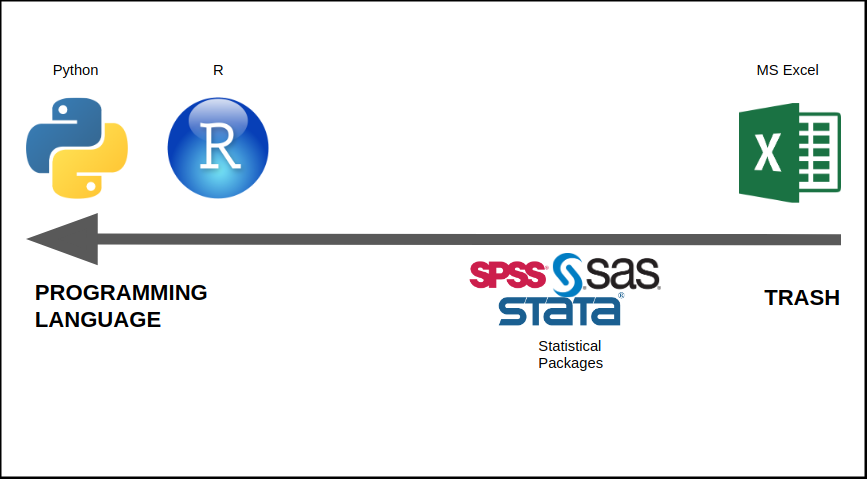
\includegraphics{trash.png}
\caption{Important Diagram.}
\end{figure}

\hypertarget{diagram-and-related-languages}{%
\subsection{Diagram and Related Languages}\label{diagram-and-related-languages}}

So, to sum this up, if you look at the diagram again from right to left: excel is a point and click tool and you should only use it for some final touches sometimes; STATA, SPSS, and SAS are the bottom of the barrel and you should stay away from them; and R and Python are both programming languages and you cant be wrong picking either.

This was an overview of what R is and how it compares to some other similar and not similar at all languages. Right now though, we do not need to know anything else about them because we will not be interacting with any of those for the first half of the book at least. Next, I would like to talk about the languages that we WILL be actively communicating with throughout this book and after.\\

There are four languages that we will be interacting with throughout this book. Do not get scared here though as they will be introduced very slowly and you should have no problems understanding what is going on at the stage of the book when we will be introducing them. I will tell you right now that these languages are called SQL, HTML, CSS, and JavaScript. Also, if you never heard of them, do not start googling them as you do not need them at the moment. Maybe, google SQL, but thats it. By the time you are finished with this book, you will have a good understanding of SQL and CSS, and some understanding of HTML and JavaScript. That will serve you well as an entry point to these languages should you decide to branch out beyond R.
Why are we introducing you to these languages?

\hypertarget{sql}{%
\subsection{SQL}\label{sql}}

Lets start with SQL. One of the things that you will be doing almost every day is interacting with a database or databases. I know, because that is what I have been doing since the second day at my R-requiring job. That is what I am still doing today and that is what I will be doing for as long as I am programming in any language. Here is a brief intro to SQL. SQL is sort of a programming language, but it really is not. It is a language that you will use to interact with databases. You can not really avoid using SQL as it is the only way to get or add data from or to a database, and if there is another way that I dont know about, then you do not need to know about it at the moment either, because it is definitely some bullshit way that nobody uses or will ever use. Just remember, SQL is your language for database interaction. SQL is important, and the best thing about it is that it is quite easy to pick up, at least the basics.

SQL is quite easy. Obviously, there is a bunch of complicated and advanced stuff that you can do with SQL, but you will not need that now. Instead, we will do some very simple pulls in SQL and compliment it with some R language to clean and aggregate our data. After you finish the book and build a few small apps requiring some basic SQL, you will obviously spread your wings and learn some advanced SQL, but that will be later. So, that was SQL. If you are really new, just like I was couple of years ago, you also want to know what is a database and why do we need it.

A database is just that, a data storage where you keep all kinds of information in a form of tables. Imagine an Excel table (If you can't imagine an excel spreadsheet, then you should really take some pre-requisites before continuing). Well, database is just a collection of such tables. Why cant we just use an excel file for our data storage needs? We could, but an excel table can only hold a little more than a million of records before it fucks up. Imagine that you are running a store that sell 1 million strap-ons every day. You will have to create a new spreadsheet every day just to keep your strap-on selling records. What if you are also selling some rifles. Your records will go out of hand very quickly and you will start losing a lot of information and instead of paying attention to your weird strap-on/ak-47 selling business, you will be worrying about your excel spreadsheets not opening. Databases solve that problem. They are built specifically to store virtually infinite number of stap-on and ak-47 records. On top of that, databases are fast and SQL language makes working with them easy. So, remember, for a lot of data (millions of rows) we are using databases and SQL. You can still, and we will, use an excel type of file to do some small jobs and share them via emails and so forth, nothing wrong with that. That is about all you need to know about SQL and databases at the moment. Lets cover HTML/CSS/JavaScript next.

\hypertarget{about-htmlcssjavascript}{%
\subsection{About HTML/CSS/JavaScript}\label{about-htmlcssjavascript}}

Cascading Style Sheets. Fancy, right? CSS is not really a programming language, it is a styling language. Every color, every curved line, sliding panel, animation, and all the fancy stuff that you see when you browse the internet or use apps is styled using CSS or at least some implementation of CSS. I mentioned that CSS is not a programming language. It is instead a part of the family of three languages, HTML/CSS/JavaScript. You have probably heard of these or at least of some of these. Basically, these three power the modern internet. Nearly 100\% of what you see when opening your browser is these languages. They DO work with other languages to do some stuff behind the scenes like shopping carts, statistics, machine learning, etc, but, generally, whatever you see in front of you is a some combination of these three languages. To cement it in your head, I want you to think about these languages as a sentence structure. HTML is a noun, it defines the object. The object being a web page. So, HTML creates a web page, just an empty skeleton, no colors, no pop ups, no styling, nothing really works yet. All you are seeing are some text, some buttons, drop downs maybe, unformatted pictures but they are not really doing anything yet. Hopefully, you see the picture. If not, check out the one below.

CSS in this setup is the adjective, in other words, it describes the noun just like CSS adds colors, lines, animation, and other visuals to that empty web page that we just created with HTML. At this point we have a nicely styled web page that doesnt really do much, which you can get away with in some cases. Below is one of the Amazon pages. You can sometimes experience the view on the right when, lets say, you lose internet connection. A server, first, loads the structure of a page and then applies the css. So, below, the unstyled page is on the right and styled on the left.

\begin{figure}
\centering
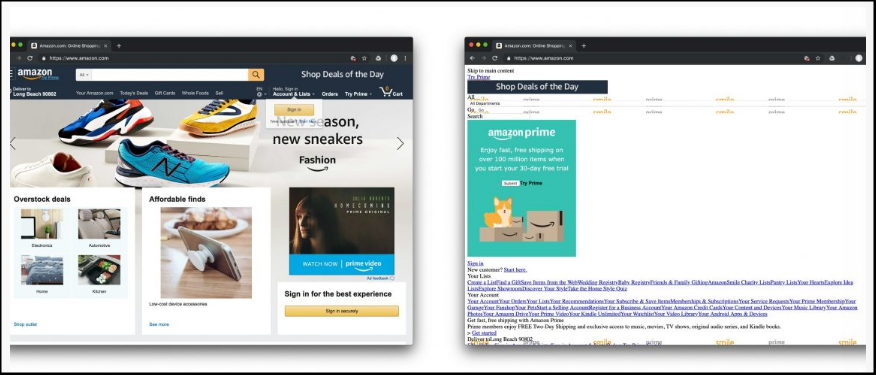
\includegraphics{csshtml.png}
\caption{Html ith and without CSS.}
\end{figure}

However, if you want your website or your app to actually do something, you are going to need JavaScript. JavaScript in this setup is a verb that defines the actions of the page that we have just made with HTML and styled with CSS. A simple example of what JavaScript does in combination with the other two is the following: HTML creates a button; CSS makes it blue and its text white and adds animation to it when it is clicked; JavaScript makes sure that when you click that button something happens, a plot is generated or a set of data is printed, or some calculation is happening and the result is shown on the screen.

\begin{figure}
\centering
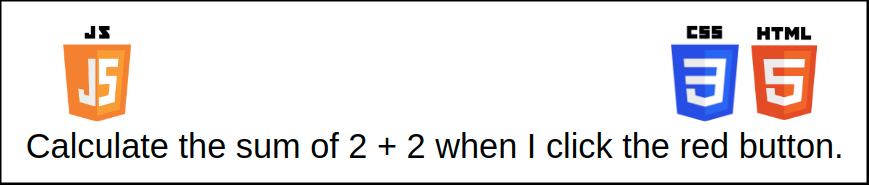
\includegraphics{jshtmlcss.png}
\caption{JS/HTML/CSS as a sentence.}
\end{figure}

Hopefully, this paints a clear picture about this family of languages and about how they interact with each other and with you.

\hypertarget{using-the-htmlcssjavascript-in-this-book.}{%
\subsection{using the HTML/CSS/JavaScript in this book.}\label{using-the-htmlcssjavascript-in-this-book.}}

We are definitely not going to touch any of these in the first book. You will be learning the fundamentals of R and will not be creating any web pages or web apps that would require styling or interactivity. You will start seeing some CSS styling starting with the second book, where we will start introducing you to the R library for creating web apps called `Shiny'.

The third and forth chapters will mostly revolve around `Shiny' and web apps and that is where we will be using CSS, HTML, and JavaScript. Fortunately, `Shiny' is HTML/CSS/JavaScript wrapped in one thing, and that is its beauty. Using `Shiny', you do not need any prior knowledge of HTML, CSS, or JavaScript. Everything is wrapped for you in the nice package and the only things that you need to worry about is the data, logic, and functionality of your app. Having said that, `Shiny' does limit you to it built-in styles and functionality. There are many auxiliary libraries surrounding `Shiny' that expand its functionality and that is great, however, sometimes, it will not be possible to find exactly what we will be going for, and that is where we will be needing lots of CSS and a little bit of HTML and JavaScript. I want to tell you ahead of time that we will not be doing a lot of HTML and JavaScript. We will use these two here and there in a form of tricks and hacks to make our apps look cool, but not more than that. The majority of our customization will be done using CSS. So, do not sweat researching HTML and JavaScript, you will not need any knowledge to keep up when we will be using it.

To sum up: we will focus on R fundamentals and some SQL at first. In the later books, as we move into web applications and start using `Shiny' library, we are going to introduce some CSS; and once we move deeper and get better, we will be using much more CSS and will be adding some HTML and JavaScript hacks and tricks to make our apps amazing.

\hypertarget{about-infrastructure}{%
\section{About Infrastructure}\label{about-infrastructure}}

Apart from R itself, `Shiny' tools, SQL, and the side languages mentioned in the previous section, there is infrastructure. Infrastructure is everything that makes the production and consumption of your product possible. Infrastructure is very important. The infrastructure that we will be covering in this and later books will include database and storage options, hosting options, API calls, optimization, and some other tools like docker and electron, which also fall under the category of infrastructure.

\hypertarget{databases}{%
\subsection{Databases}\label{databases}}

We have already covered some ground on databases and SQL. However, there is a second side to databases, actually building your own database. In that scenario, you are serving as a data engineer providing infrastructure for yourself or for others. I will teach you to do that in the next books. You will use our database in this book. But I am jumping ahead right now, you dont need to worry about this now, and we will have a deeper dive into this topic somewhere in the third book.

\hypertarget{hosting}{%
\subsection{Hosting}\label{hosting}}

Imagine that you have just built your first app. It is now on your computer and you can play with it .Very cool, except, nobody else can really see it besides you. Your app has to live somewhere else besides your computer, and hosting accomplishes just that. Hosting lets you release your product to the public. Same applies to web sites and databases by the way. Good news is that there are free options for your hosting and you can even set up your own hosting straight from your home computer. Hosting and databases go hand in hand and will be two most important infrastructure topics in the following books. Other things will kind of revolve around these two.

\hypertarget{other-tools}{%
\subsection{Other tools}\label{other-tools}}

In the fourth book, we will start introducing more advanced concepts and tools like api calls, dockerized apps, optimization and some others. Even though I called these tools advanced, it doesnt mean that they are hard. In fact, they are much easier to pick up once you are ready. The reason they are in the advanced category is that you must first learn all the things that I have been talking about up until now before you even need to know what these `advanced' things do, purely because you just do not need them in the beginning.

That was our brief introduction into the topic of infrastructure. The coolest thing about infrastructure is that it, maybe, sounds boring at first. You are thinking, `I just want to create something cool. And apps are what I and everybody see and that is why it is cool.' Well, my answer to you is, `You will be surprised'. You will be surprised by how exiting it is to build your own database for the first time, connect to it, load and pull some data, and for all this to work. Or to set up your hosting, put your app there and open it from your phone and start sending that shit to your friends to brag. You will see, just like I did! All I am saying is dont assume that `back-end' (nerd term for the infrastructure that we are talking about now) is something boring or something you dont want to be doing. I can almost guarantee that once you built your first few apps and showed them to people, you will be more exited to talk about the stuff behind that app, the stuff that makes it run. The picture in front of peoples eyes (`front-end') will become a `noob' stuff at that point.

\hypertarget{about-me}{%
\section{About Me}\label{about-me}}

In this section, I think, I am trying to relate to you, a person with no computer science degree. It is a general idea that coding is hard. And what I say to this is, `It is absolutely CORRECT'. Coding is incredibly hard and all those asshole pretend gurus on youtube that say `learn xyz language in 20 minutes or 5 hours or 1 month' are fucking lying. Those videos are click baits and they will not teach you shit. It will take you at least 4-5 months of consistent everyday work to get to the initial comfort level.

Now, having said all that downbeat stuff, I want to assure you that you do not need a computer science degree to become a professional software engineer or a data engineer or a database engineer. I do not hold a computer science degree, yet, I have been quite successful at this and feel qualified to teach you this stuff. But what about those people who went to school for this? First of all, you should only worry about your own skill as there will always be better programmers than you. So what? The demand for coding specialists will only increase and there will never be enough people who programmed since kindergarten. That is where YOU come in. Secondly, what do you think kids at college do? At best, if they are full-time, they go to school twice a week, take two coding classes at best (A WEEK), then some other two useless classes like underwater poetry and hipster studies just to graduate. After that, they go home and jerk off for the rest of the week or play video games or both. Only a minority will actually commit an appropriate amount of time to learning code. What do you think they know in the end? Obviously, they are going to have some fancy resume that will say something like Python, C++, JavaScript, PHP, blablabla. But when you sit them down and ask to build something, they will be lost a lot of times. It is not to say that there is much wrong with learning at the job, it is just I do not want you to operate under assumption that you are so far behind that it is impossible to catch up.

I recently watched a documentary about hackers and companies guarding against them. In that documentary they showed unpaid guys in their hoodies, hacking and learning from home every day almost all day, way past nine to five with real commitment and intent, just for fun. At the same time, they show a private company with a bunch of college graduates-programmers struggling to prevent their clients from hacker attacks. You can see all that nice equipment, interactive maps, and so forth. But they still lose to those hackers a lot of times. Why is that? The reason is dedication. I am sure there are exceptions, but just like with college students, majority of employees are there nine to five, they will take any break possible and are really looking forward to that work day to fucking end or to accumulate enough vacation days to get the fuck out for a while. The hacker bro, on the other hand, sits there and learns relentlessly about some new cool way to fuck someone up. You would say, `but he is outnumbered'. In programming, you are only as good as the number of hours that you have coded, not the number of degrees you got or years you have spent to get them. That hacker does not need to spend more hours programming than the whole team of that company combined, just more than their best programmer. In that situation, it is like a case of zero multiplied by any number is still zero. If that hacker is much better than their best person, he will run circles around them and they wont be able to do much. This little story is just my way to cement something in your head. Unlike medical or legal fields, in coding, you are only as good as your code. And the only way to improve is to code. Certificates alone will not get you very far.

\hypertarget{nikita-voevodin}{%
\subsection{Nikita Voevodin}\label{nikita-voevodin}}

So, what makes me say with confidence that you do not need a degree to succeed at this, and moreover, what makes me qualified to teach you all these things. Well, this many pages into this book, I would like to introduce myself. My name is Nikita Voevodin, I am a professional data analyst and software developer with concentration in interactive visualizations and database setup. I spent the last half of the decade doing legislative, budget, policy, and data analysis for New York City and New York State. My work involved developing and automating big data processes, building and interacting with databases, creating apps and dashboards for my superiors and public, as well as conducting high level research to empower legislation in the area of city transportation. I hold three separate degrees, BS in economics, BA in political science, and MPA in public policy. As you can see, I do not hold a degree in computer science or anything related. In fact, apart from having a PC since I was 9 and using it mostly for games, and learning some excel in college, I had no coding background of any kind. I never even knew anybody who coded. This book is the chronological representation of my progress from zero to the quite high level of proficiency. Now, what makes me qualified to teach you? Ultimately, you will be the judge of that, but I would also like to list some of my portfolio items in R. First, I went from knowing practically nothing about programming to doing some advanced stuff within a year. Secondly, I am an author or co-author of R Shiny apps like \href{https://tlcanalytics.shinyapps.io/tlc_dash/}{TLC Data Hub}, \href{https://tlcanalytics.shinyapps.io/decoder/}{TLC VIN Decoder}, and the \href{https://tlcanalytics.shinyapps.io/tasks/}{TLC Data Meetup App}, components from which will become the base for this and the following books. Finally, I have built databases, countless algorithms, and have completed multiple large data analysis projects for different agencies within the City of New York. Most importantly, I taught all these things to myself, I have clear understanding of what it is like to start from scratch, and I have a vision of how a completely new to programming person should start learning code.

\hypertarget{flow-of-this-book}{%
\subsection{Flow of This Book}\label{flow-of-this-book}}

As I said before, coding is mostly dry and dull subject for most people. My goal, therefore, is to keep your attention and interest for as long as possible. Besides bad words and seasoned jokes, I decided to add an element of a strory telling. The story will not be present everywhere, because there are some basics that we just must run through. However, I will try to keep the whole thing in the boundaries of the story, which, in the first book, is based on my first three - four months of learning R. Lets go.

\hypertarget{first-three-months-maggot}{%
\chapter{First Three Months (Maggot)}\label{first-three-months-maggot}}

Congratulations, you just accepted that job offer and just waiting now for the date to start. The job description said that you need some experience working with data and some good excel knowledge, but during your interviews you noticed something: your interviews were more on the technical side and a lot of people in the office are using those dark screen hacking terminals that you have only seen on TV. Nobody is yet telling you that you need to learn programming but now you are suspecting that you will probably have to.

Disclaimer: I do not expect your situation to be similar. It doesnt have to be. You might be looking for a job and just trying to improve your chances, or you do have a job but just want to acquire a new skill, or something like that. To keep this book somewhat interesting, as I mentioned before, we will follow my path to R proficiency. Hopefully, you will be able to relate to my story and it will keep you engaged.

Anyway, you sit home and google some R tutorials and do not really know where to start. Before I list some good resources that I used to start, we are going to need to install R and R Studio on you computer. First, what is the difference between R and Rstudio? R is a programming language just like any other language, before you start using it, it has to be installed. If you ever played video games on your computer, you should be familiar with those fucking messages like: `install the latest C++ dll something' . Basically, when you see this message, it means that the programming language that your game runs on is not there or is outdated. Once you install that update, your game runs. Games are built using computer languages (usually, something like C++ or C\# for big games and Java or Python for small ones). When you are playing a game there are scripts running in the background that you do not even see. Same is needed to start coding. In our case, we need to install R. What is Rstudio then? Rstudio is basically a notepad (also called text editor) that understands R language and makes it run. There are many such notepads out there, however, Rstudio is built specifically for R and that is the one you should use. Once you develop your skills a bit more, you will start looking at other text editors (notepads). For example, the most popular general use text editor right now is Visual Studio Code. You could use it for R but it is not built for data analysis and it will be very inconvenient for you to use, at least in the beginning. So, do not worry about it at the moment. We will be using Rstudio. Lets jump straight into the installation process.

I am not going to hold your hand too much during the installation process. If you want to actually learn to code, some things you will have to figure out on your own. Both, R and Rstudio will run on every major operation system. For example, I am using Linux Ubuntu, but I also have them installed on my windows PC at work, and I previously used them on MAC as well. Once installed, everything will run just the same on any platform. So, go to \href{https://mirror.las.iastate.edu/CRAN/}{one of R repositories} to install R.

\begin{figure}
\centering
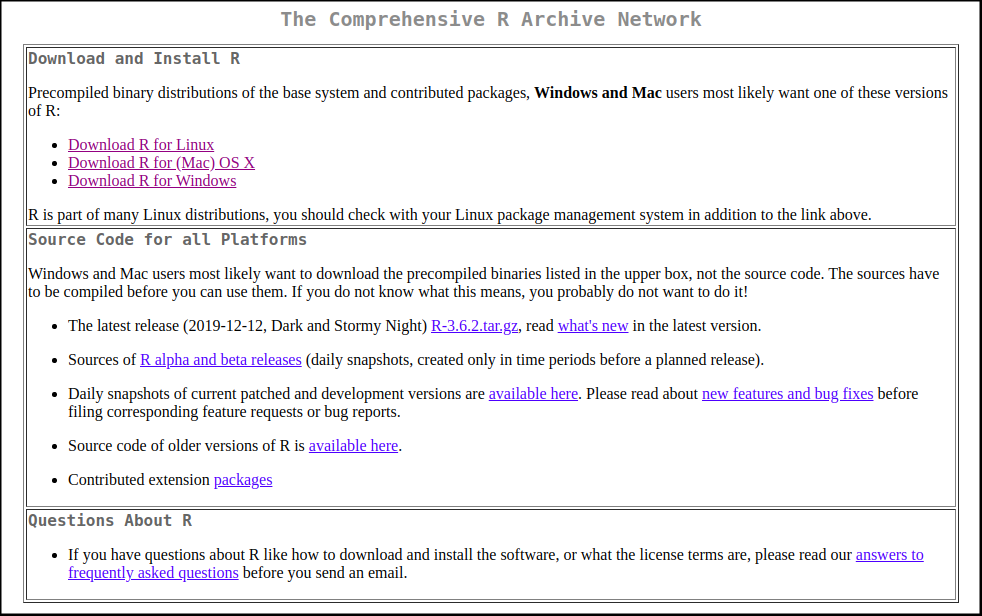
\includegraphics{rInstaller.png}
\caption{Downloading R.}
\end{figure}

After that is done, go to the \href{https://rstudio.com/products/rstudio/download/}{Rstudio page} and install the latest Rstudio for your system.

\begin{figure}
\centering
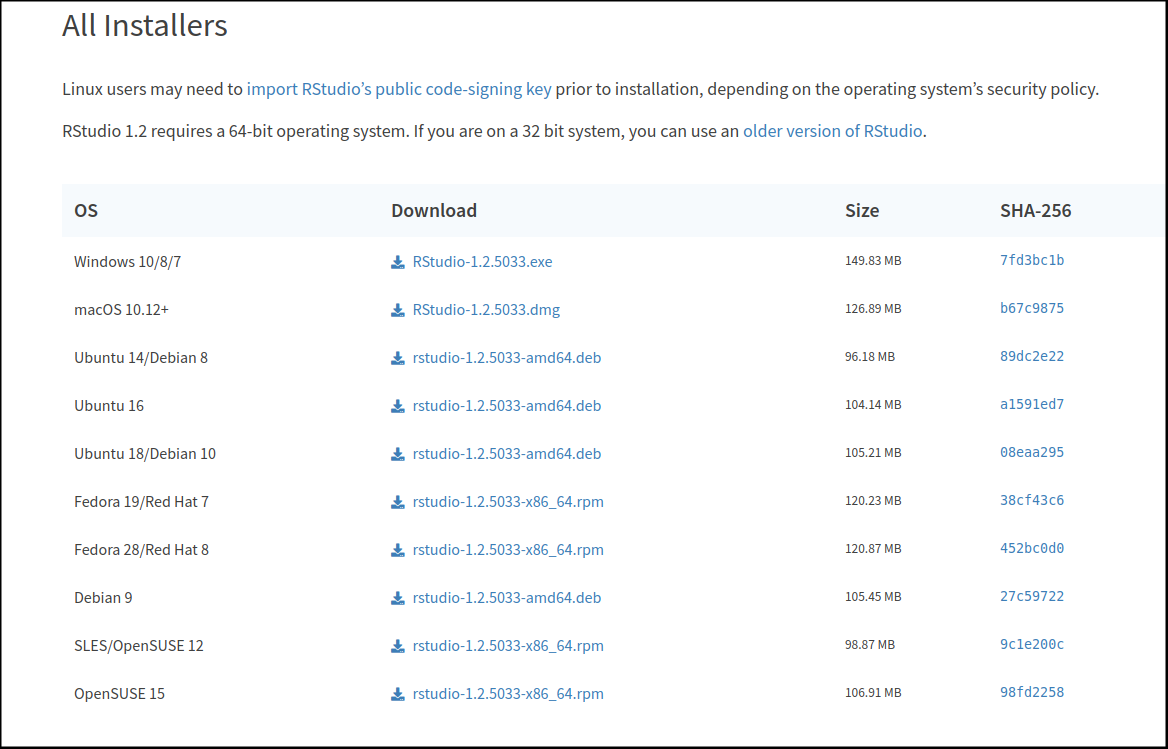
\includegraphics{rstudioInstall.png}
\caption{Downloading RStudio.}
\end{figure}

That is it. We are ready to start coding. Well, in your case, let the horrible grind of the first few weeks begin!

\hypertarget{messing-around}{%
\section{Messing Around}\label{messing-around}}

Your Boss sits you down and tells you: play with r for a while I will give you your first task in a couple of days. Your first few day at the job are slow and encouraging. You are meeting new people and everything is nice. Things are being installed on your computer and, for now, you are just reading some literature about your organization and some latest initiatives. Your boss gives you some space to settle down and play around with your new setup. He tells you that your first task will be cleaning some of his old code. To your naive ears it sounds like, `Take your time, your first assignment will be easy, you will just add some commas and some narrative to my code. Nothing to worry about.' And you sit down and start messing around with R.

\hypertarget{first-script}{%
\subsection{First Script}\label{first-script}}

First thing to do is to open the Rstudio. When you open it for the first time you should see something like this:

\begin{figure}
\centering
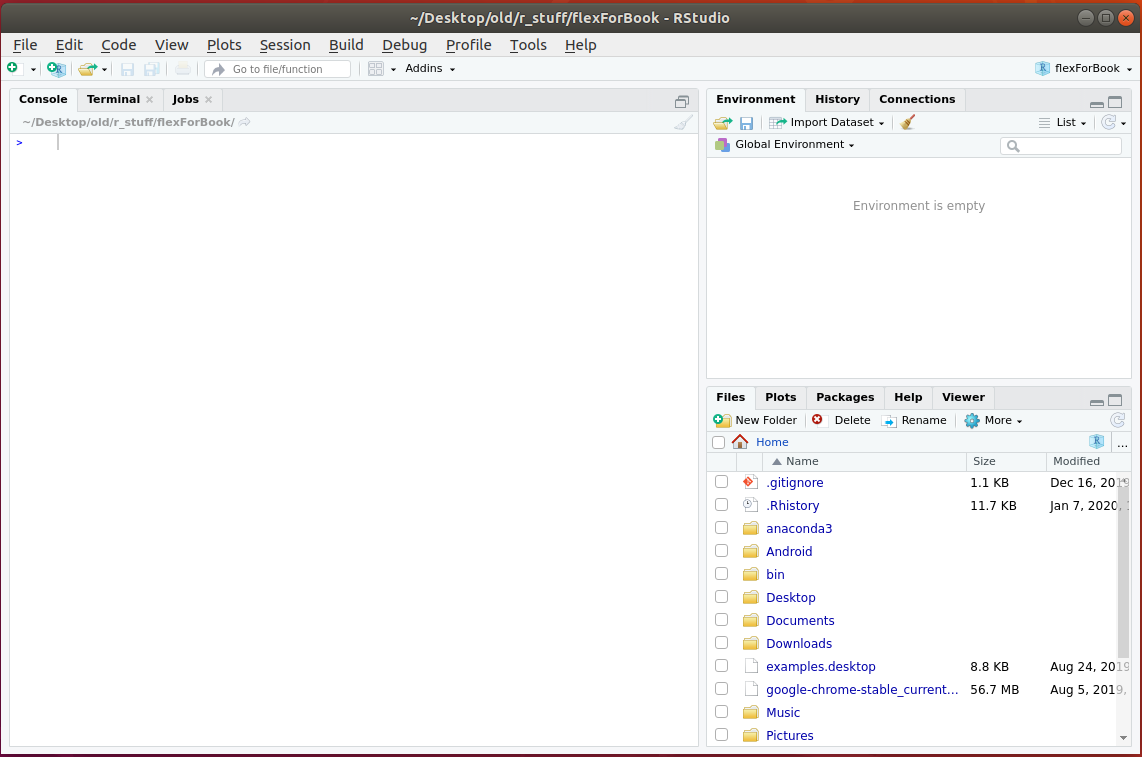
\includegraphics{rstudio.png}
\caption{RStudio.}
\end{figure}

Go ahead and create your first script. For that, go to the upper left corner, click on the + icon, and chose the `R script option', which should be first. You should see something similar to the picture below. Get used to this view as it will be the one you will be seeing a lot from now on.

\begin{figure}
\centering
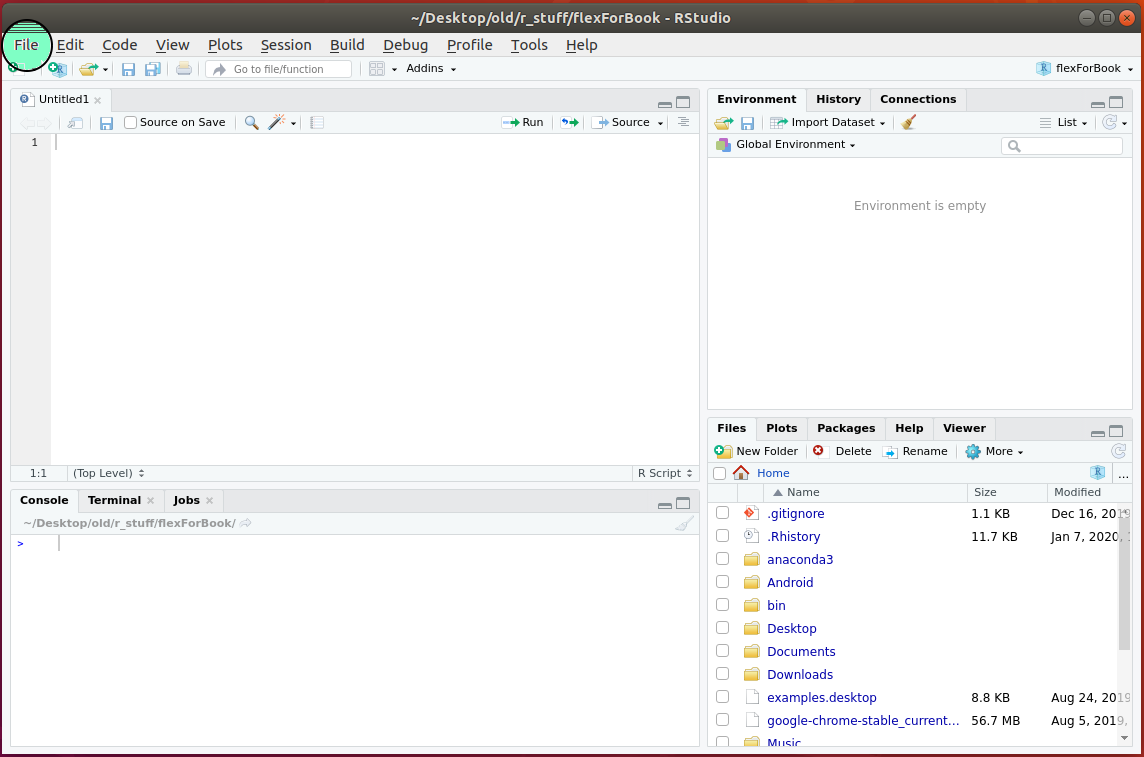
\includegraphics{rstudio1.png}
\caption{RStudio.}
\end{figure}

\hypertarget{layout}{%
\subsection{Layout}\label{layout}}

Rstudio is quite a complicated text editor. It has a shit ton of advanced features and many settings. I myself dont even know most of them, and absolutely encourage you to look into them once you know what the hell you are doing. And since, right now, you probably dont know what the hell you are doing, you will only be focusing on things that you need to start. There are only four areas of the screen that you need to know about now. And I also drew it for you on the screenshot. The first screen is where you will be writing your code. This is your main area. Go ahead and write this:

\begin{Shaded}
\begin{Highlighting}[]
\NormalTok{      myFirstLineOfCode <-}\StringTok{ 'This is my first line of code!'}
\end{Highlighting}
\end{Shaded}

\begin{figure}
\centering
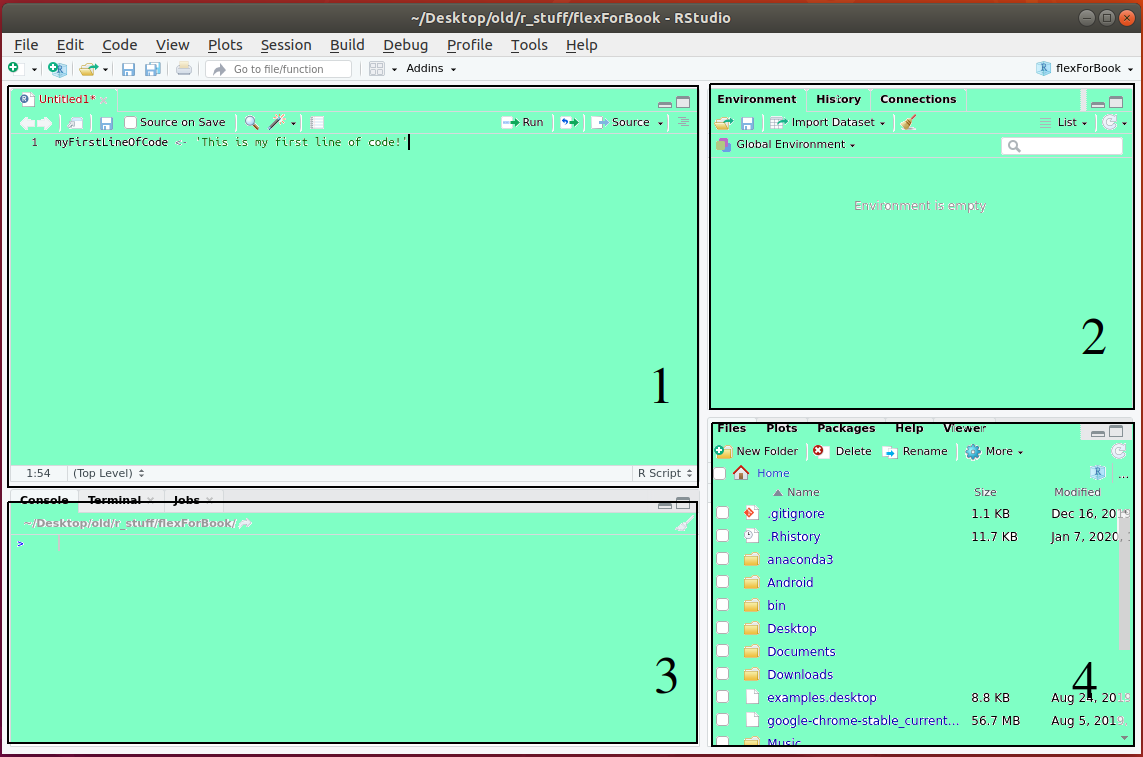
\includegraphics{rstudio2.png}
\caption{RStudio.}
\end{figure}

Click `Run' (the upper right side of the main area). Instead of clicking `Run' every time, you can just highlight the chunk of code that you would like to run and press `Ctrl + Enter'. Also you can just click anywhere on the code that you want to run and press `Ctrl + Enter', same thing. Go ahead, and try all three. A couple of things just happened. In the area number two, you should now see the variable `myFirstLineOfCode' as well as what is inside of that variable - `This is my first line of code!'. In this window you will be seeing all the variables, tables, and other data that you created or imported. Whatever is available at the moment.

\begin{figure}
\centering
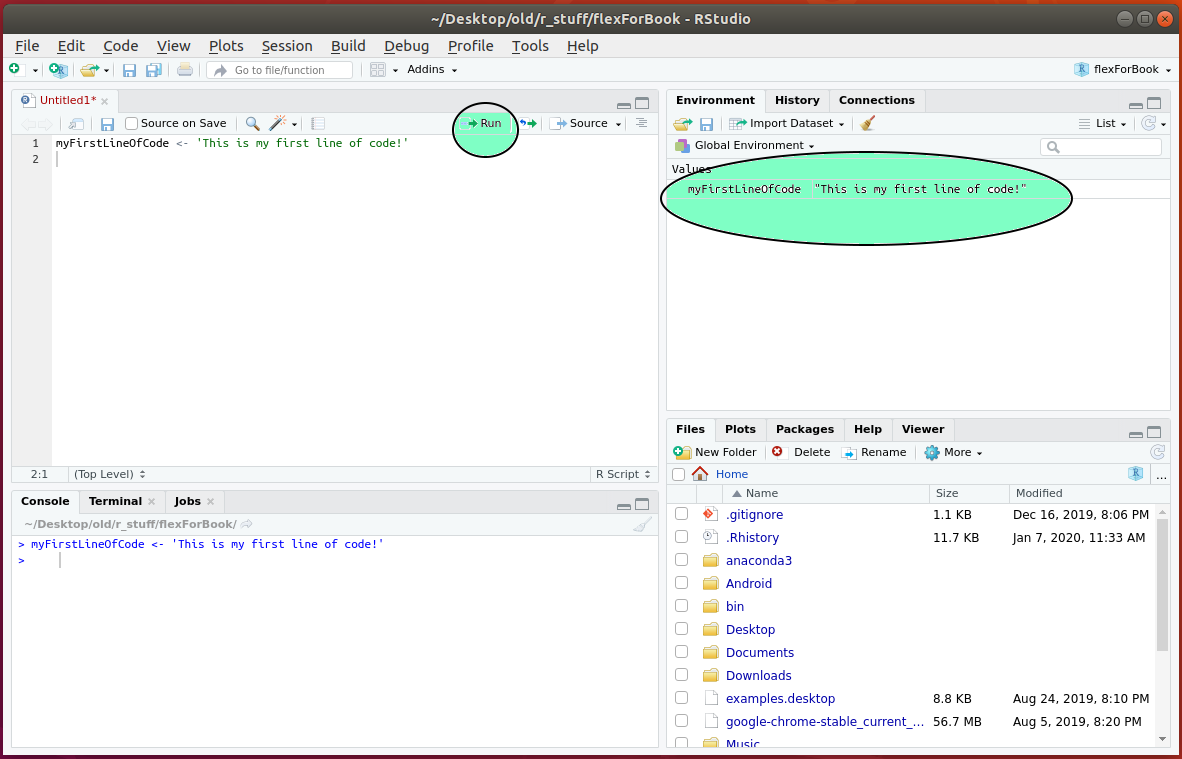
\includegraphics{rstudio3.png}
\caption{RStudio.}
\end{figure}

What else happened? In the view number three, you can see the code that you ran. If you ran it three times, you would see it three times. The main use case of this area for us is to check if our code is running, finished running, or generated errors or warnings. Lets generate an error. Type your name without parentheses in the view number one and run it. It should generate an error in the view number three (something like : `Error: object 'Nikita' not found').

\begin{figure}
\centering
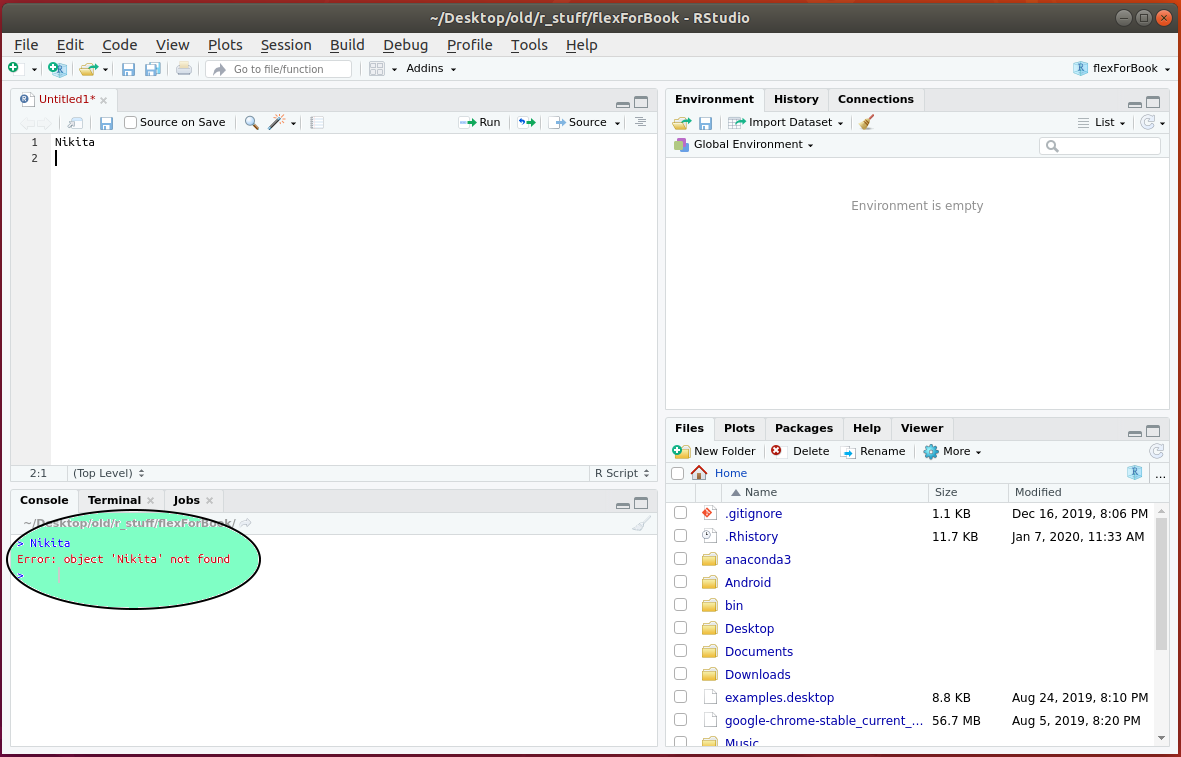
\includegraphics{rstudio4.png}
\caption{RStudio.}
\end{figure}

Just like this, we know something is wrong with our code. This is not all the third view can do, but this is how we are going to be using it. Just for the sake of awareness, I would like to show you what else it can do. Type this in the third view:

\begin{Shaded}
\begin{Highlighting}[]
\NormalTok{  test <-}\StringTok{ 'testing the third view'}
\end{Highlighting}
\end{Shaded}

\begin{figure}
\centering
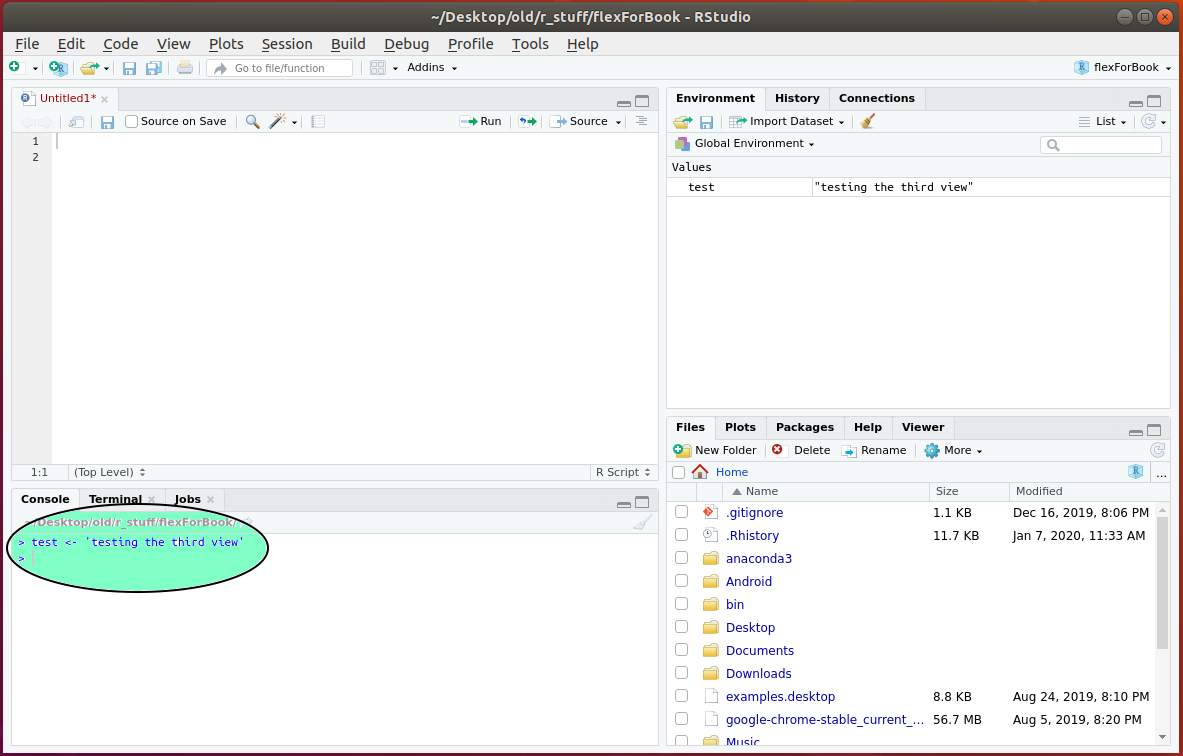
\includegraphics{rstudio5.png}
\caption{RStudio.}
\end{figure}

Hit `Enter'. See? Same as the main view, it ran this code without clicking `Run' or `Ctrl + Enter' and stored the result in the second view. The difference is, that code is now gone. It is useful to test your code or to run something quickly but we wont be using it now. Just wanted to show it to you. Now, lets look at the view number four.

\begin{figure}
\centering
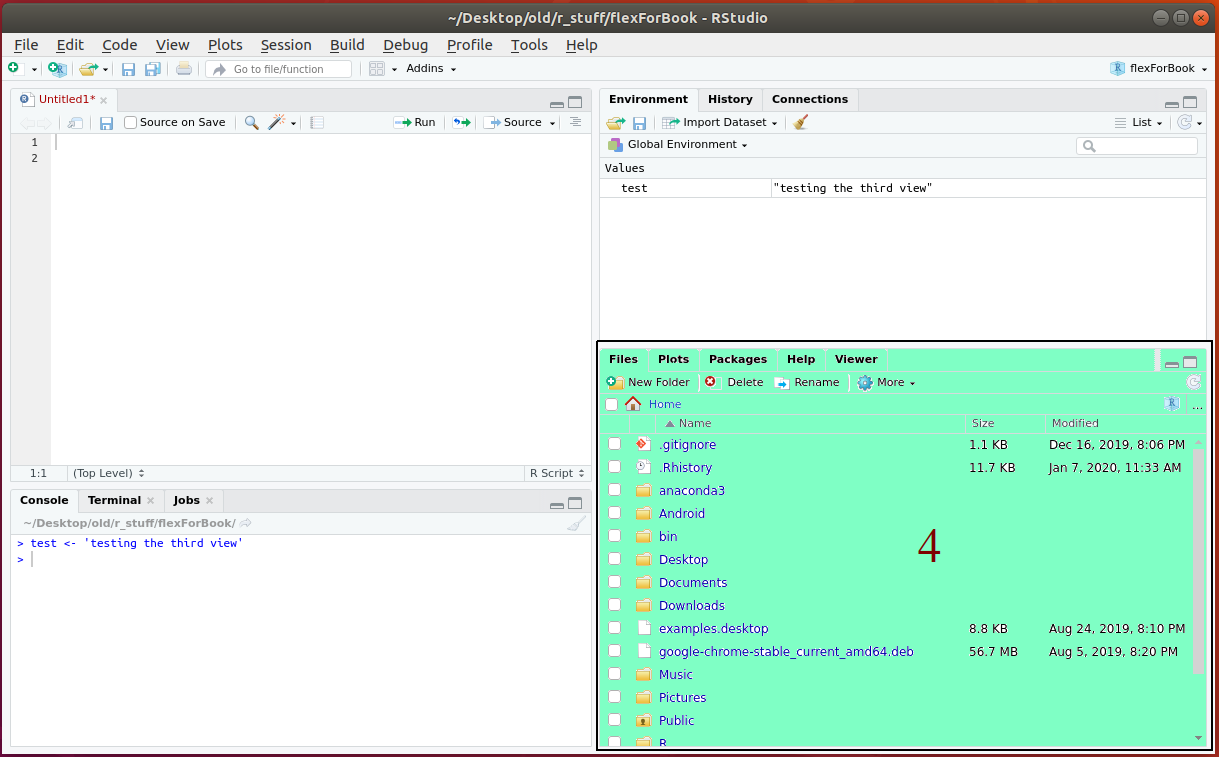
\includegraphics{rstudio6.png}
\caption{RStudio.}
\end{figure}

This view will not be super useful for us now, so, dont worry about it now too much. Basically, now, you should be seeing the folder that you are currently in. Also, when we will be creating graphs and maps, they will appear there. That is about all you need to know about the fourth view right now. In fact, this is about all you need to know about the layout. Lets move on.

\hypertarget{saving-r-file}{%
\subsection{Saving R File}\label{saving-r-file}}

Now, lets save this file and see where it goes. When you are new, or using a new tool, there is always that fear that you will break something and will not be able to get it to work again. One thing I want to do right from the start is kicking that fear out of you. To do that, in this and the next few sections, we will try to do some things that will seem damaging to your setup. I will show you that you can not really do much damage or lose a lot of data by doing routine operations and if something really went wrong, how you can restore things. So, go ahead and save our script by clicking the floppy disk icon on top (I hope, I do not need to explain to you how to save files. This operation is pretty universal).

\begin{figure}
\centering
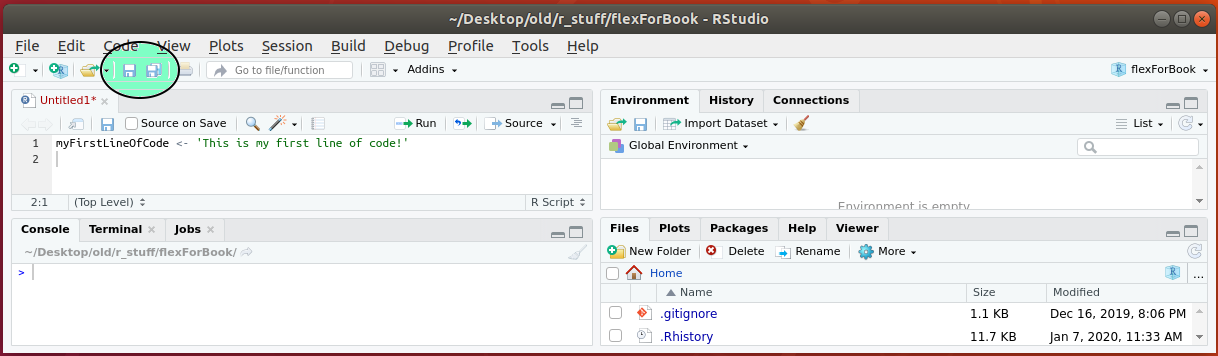
\includegraphics{rstudio7.png}
\caption{RStudio.}
\end{figure}

Now, close the Rstudio. Go to the folder where you saved your file and open it. You should be where you left off.

\hypertarget{simulating-a-problem.}{%
\subsection{Simulating a Problem.}\label{simulating-a-problem.}}

Now, lets simulate a problem. Lets see what happens if your Rstudio session freezes or your computer just crashes. So, lets add another line of code to our script and see what happens if we forget to save it and windows fucks up again. Go ahead and add this line of code right under the first one:

\begin{Shaded}
\begin{Highlighting}[]
\NormalTok{mySecondLineOfCode <-}\StringTok{ 'This is my second line of code!'}
\end{Highlighting}
\end{Shaded}

Run it. I hope you remember how. Now, do me a favor, open the activity monitor by pressing `ctrl + alt + del' and selecting it if you are on windows. Kill the Rstudio process.

\begin{figure}
\centering
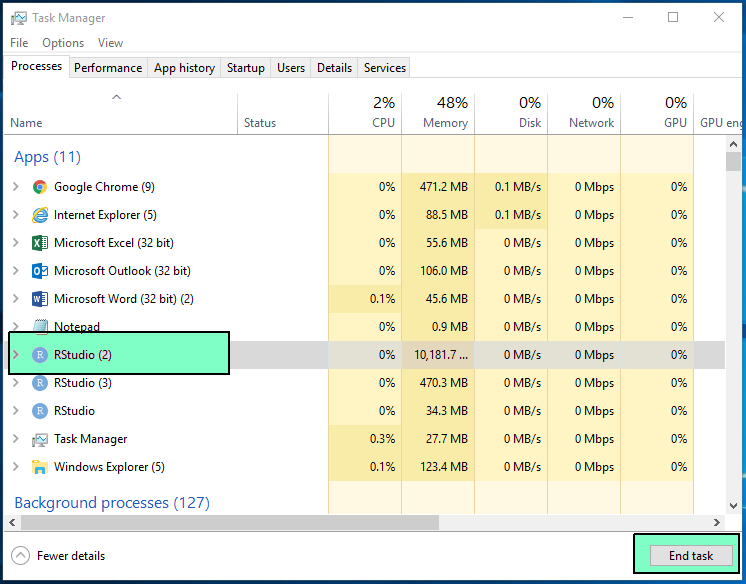
\includegraphics{rstudio8.png}
\caption{RStudio.}
\end{figure}

We never saved our code, and imagine if you had some hundreds of lines of code that you never saved (obviously, that would be stupid, but happens). It happened to me a few times with excel and word, and I did not have autosave enabled and I lost some good number of hours of my life rewriting my shit, because windows decided to fuck me. Fortunately, this will not happen to you with Rstudio. Now, do not open the file that you saved, instead just open Rstudio again. Yes, you need to open a completely new Rstudio session. If you are on Windows for example, go to start, find Rstudio and click on it, if it is on your desktop, open from there. It should open with that second line there. We just simulated a hard stop of your Rstudio session and that should eliminate some portion of the fear about losing your progress. Things like that happen more often than you think. If you are loading more data than you RAM can handle or if you have a weak CPU, chances are you will see freezes quite often. You will have to deal a lot with restarting your computer and reopening R sessions. Your code in most situations will still be there.

\hypertarget{re-installing-rstudio}{%
\subsection{Re-installing RStudio}\label{re-installing-rstudio}}

When you are just starting, you are going to end up experimenting with your setup quite a bit. That might or might not lead to breaking things or at least to having it working not the way you would like it to. What do you do? Just not experiment? Not really. It is just like with learning to ski or snowboard, first thing you need to know is how to stop. If you learn how to stop first, then, no matter what, you are safe, you will not break your neck. Same here, when you know that you can always start from scratch, you are in control, and you learn faster. So, lets imagine that we did something that made our Rstudio setup really unusable for us. There is nobody to help us. What do we do? Delete this shit and reinstall. Proven method, patented by myself. Go to your control panel if you are on windows and delete Rstudio. If you are on MAC, just drag it to the trash. If you are on Linux, I expect you to know what to do. Now, just follow the steps that we used to install it. When you open it, you will have a clean Rstudio, but you will still be able to easily access all code scripts that you saved so far. Go ahead and open your new Rstudio. Once opened, go and open that script that we have saved. You should see the same line of code that we had:

\begin{figure}
\centering
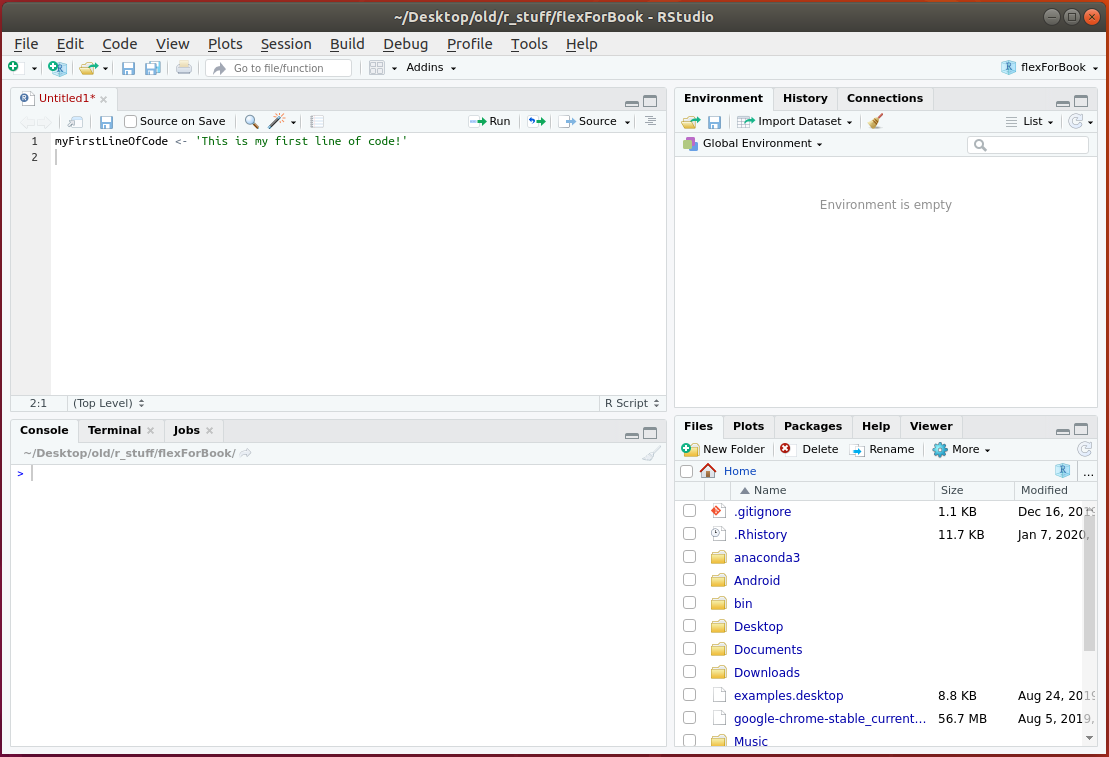
\includegraphics{rstudio9.png}
\caption{RStudio.}
\end{figure}

\hypertarget{messing-with-packages}{%
\subsection{Messing with Packages}\label{messing-with-packages}}

As a final step of kicking the fear of screwing up your setup, we are going to install a few packages, remove them, and also, manually remove them. Quickly about packages. Packages and Libraries are used interchangeably in R, they mean the same thing. Any Joe Shmoe can write and publish a package in R, given enough knowledge. Package is just a collection of functions that make your life easier. It can even be just one function. For example, R has a number of built-in functions like `read.csv()' for reading csv files. Some guy thought that he could do better and wrote his own function that reads CSVs faster and gives you more options. That function is called `fread()', and it is a part of the `data.table' package. In order to use `fread()', you first need to install the `data.table' package. There are tons of packages out there and we will be using a lot of them. Packages for files, maps, aggregations, graphs, web apps, etc. I hope you are getting it so far, we are going to dive deeper into packages a bit later. For now, lets just install a few. Go to the top of our script, even above our first line of code. Yes, just move it a few lines down. Write this:

\begin{Shaded}
\begin{Highlighting}[]
\KeywordTok{install.packages}\NormalTok{(}\StringTok{'data.table'}\NormalTok{)}
\KeywordTok{install.packages}\NormalTok{(}\StringTok{'dplyr'}\NormalTok{)}
\KeywordTok{install.packages}\NormalTok{(}\StringTok{'shiny'}\NormalTok{)}
\end{Highlighting}
\end{Shaded}

Highlight all three entries and ether press `ctrl + Enter' or just click `Run'. You will see a bunch of cool looking installs going on. Wait till everything is done. Now, how do I tell that it is done? In the top right corner of the third view you should notice a red circle with sign stop on it. You will only see it when RStudio is busy, in other words, when something is running. Once that red button goes away, that means it is done. Now, these three packages are installed and you do need that code there anymore. Erase those three lines and instead write these three:

\begin{Shaded}
\begin{Highlighting}[]
  \KeywordTok{library}\NormalTok{(data.table)}
  \KeywordTok{library}\NormalTok{(dplyr)}
  \KeywordTok{library}\NormalTok{(shiny)}
\end{Highlighting}
\end{Shaded}

Highlight these three now and run them. And thats it, you installed and now loaded your first three packages or libraries if you want to call them that. Your session should look like this now:

\begin{figure}
\centering
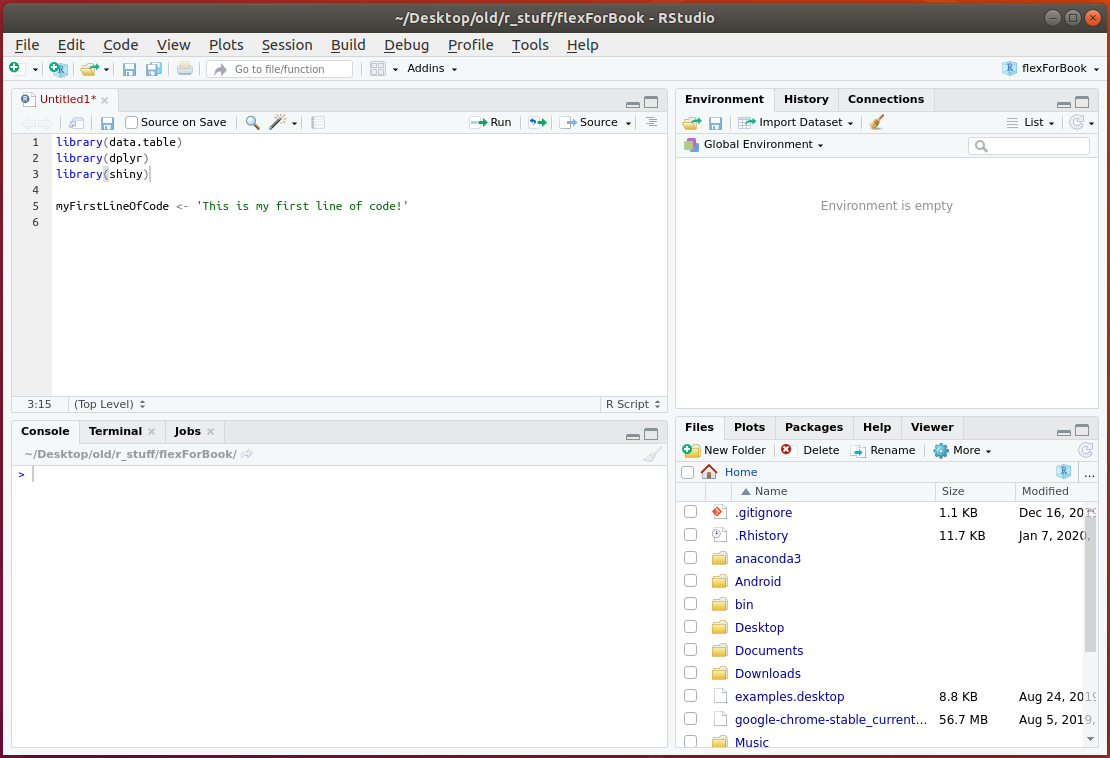
\includegraphics{rstudio10.png}
\caption{RStudio.}
\end{figure}

Now it is time to uninstall these. You would ask, why? Why the hell not? But seriously, there are two reasons. First of all, I want you to know how, and secondly, sometimes a package may conflict with another package resulting in your code messing up. Sometimes a package just wont update and will start kicking errors, and other things of that nature. It is not always straightforward and obvious what is happening. We will be installing so many different packages that one day everything might be working smoothly and the next day you code is just not running.Then, you end up just like Nicholas Cage in `Gone in 60' talking to your code just like he did to Eleanor - `Come on baby, dont be like that, please work'. To make sure you dont sit there for too long, like I did, figuring that shit out, I will teach you a few troubleshooting tricks. So, lets come back a bit to uninstalling our packages. Run the following:

\begin{Shaded}
\begin{Highlighting}[]
\KeywordTok{uninstall.package}\NormalTok{(}\StringTok{'data.table'}\NormalTok{)}
\KeywordTok{uninstall.package}\NormalTok{(}\StringTok{'dplyr'}\NormalTok{)}
\end{Highlighting}
\end{Shaded}

Erase these two lines. If it worked, running the following will not work, because packages are not there anymore:

\begin{Shaded}
\begin{Highlighting}[]
\KeywordTok{library}\NormalTok{(data.table)}
\KeywordTok{library}\NormalTok{(dplyr)}
\end{Highlighting}
\end{Shaded}

Good. What about the third one? Lets simulate another problem. At some point, eventually, you will encounter a strange piece of shit error -- you will be trying to load a library, but it will say that there is no such package or some shit. You will then try to install that package and it will either install it or will tell you that that package is already installed. You will then try to load the library, but the same fucking shit will happen again and again and again. You will be like, `WHAT DA FUCK?! YOU ASSHOLE!. You will then try to do what we have just done and will try to uninstall that package. It might say something like: `package is not there and can not be uninstalled' or it will uninstall it but when you repeat the whole circle again, same result. What is happening? You might have opened a second RStudio session at some point and it started installing packages to different folders. You do not have to completely follow this logic. Just remember. If something of this nature is happening to you, here is how to fix it. We are going to locate the folder where our packages age getting installed into. Then, just find the package folder in question and fucking delete it. It might tell you that the folder is in use and can not be deleted, just restart your computer and delete it after. After that, open your script that you had the problem with, install that package, and load the library, everything should work fine now. So, lets do it for the `Shiny' package. Save your script, close RStudio. If you are on Windows, your R folder should be in the Documents. So, go to Documents/R/R-\ldots{}/ and delete the `shiny' folder. If it is in use, restart your pc, come back and try deleting again. Lets confirm. Open your script again and try:

\begin{Shaded}
\begin{Highlighting}[]
\KeywordTok{library}\NormalTok{(data.table)}
\KeywordTok{library}\NormalTok{(dplyr)}
\KeywordTok{library}\NormalTok{(shiny)}
\end{Highlighting}
\end{Shaded}

Non should work, because we uninstalled the first two libraries in the previous steps and the `shiny' library manually. That is it. This is how you do a soft and a hard delete of your packages. This concludes our R-fear exorcism ritual.

\hypertarget{dark-mode}{%
\subsection{Dark Mode}\label{dark-mode}}

One thing that you must do, and I cant emphasize `must' here enough, is to switch your RStudio color theme to a dark mode. If you dont do this, your code will not work. On top of that, people will think that you are noob. The darker your screen is the better coder you are. Proven by scientists. This is a joke, of course, but, I do want you to change to the dark mode. From experience, it helps you focus better and keeps your eyes more relaxed. Also, it does look like you know what you are doing if your screen is dark. It shows that you are advanced enough to tinker with the text editor settings. When others see you as advanced, you are automatically create that level of expectation for yourself to get better, which, in turn, speeds up your progress. Every time that I helped some of my colleagues at work with their code, by far the most painful part of the experience for me was looking at their bright noob screens. Therefore, go to the `Tools' on top of the Rstudio → Global Options → Appearance and in the editor theme pick `cobalt'.

\begin{figure}
\centering
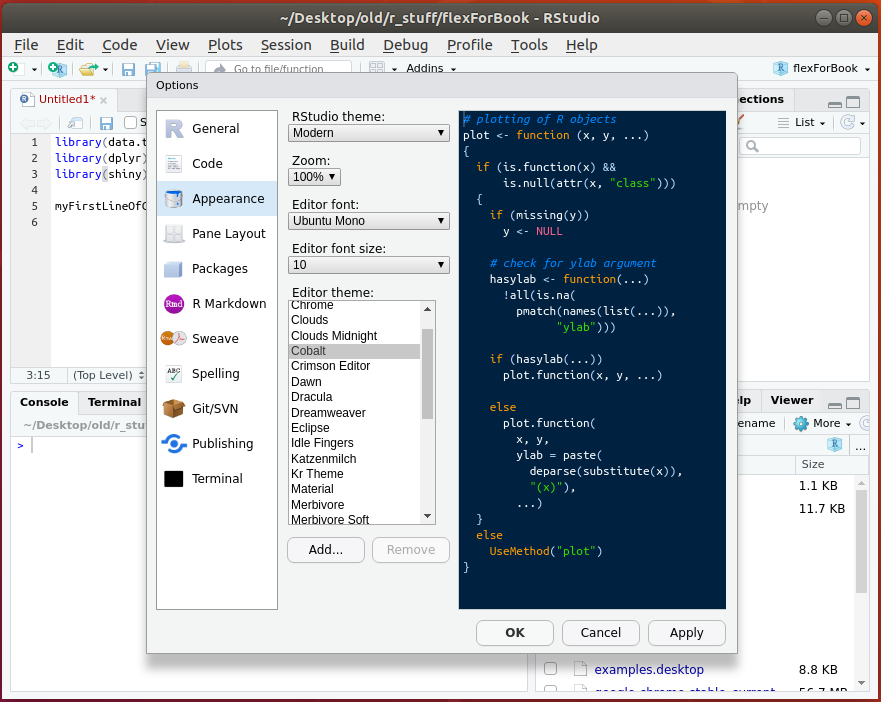
\includegraphics{rstudio11.png}
\caption{RStudio.}
\end{figure}

That is it. All that ranting was just for this. Now, this book will have the white theme. Why? Because when I will decide to publish I dont want to spend a fortune on color, that would be stupid. But you should know, I will be creating illustrations for this book wearing sunglasses. What a hypocrite, right? Maybe I will switch to cobalt as well later. You will notice if I do.

\hypertarget{second-r-session.}{%
\subsection{Second R session.}\label{second-r-session.}}

Another trick I want to show to you is using multiple RStudio sessions at the same time. You see, R is a single process language, which means that it can only tackle one command at a time. Commands are the lines of code that we were just running. The following is a command:

\begin{Shaded}
\begin{Highlighting}[]
\NormalTok{mySecondLineOfCode <-}\StringTok{ 'This is my second line of code!'}
\end{Highlighting}
\end{Shaded}

Each assignment like this, or a call to a function (like install.packages() or library()) is a command and is processed one at a time in the order that you have written it. In most cases, you will never even notice or it wont be a problem, because it is so quick. However, there are going to be many many many cases when a command will be taking an insane amount of time, and you will have to sit there like a steaming piece of shit and wait for that command to run before you can execute the next one. In most cases, a command that would take a long time to run is something like a SQL call to some old and slow or just overloaded database. I have wasted some good hours of my life interacting with such piece of shit databases. Sometimes, I waited for one to four hours at a time for my SQL command to run before I could continue. In the most extreme cases, I had to leave the script running overnight to come back in the morning to see that It has not finished, and be like: `FUUUUCK!!!'
. API calls will give you similar issues, but less often.

Anyway, do not be super afraid as it does not happen all the time, especially in the modern setup, and when it does, it is not really your fault. There is not much we can do to make a process to run faster. When you become a little bit more advanced, you will be able to, maybe, break your database pulls into segments to speed them up a bit and to have more control over them. You can also, sometimes, use parallel processing to assign tasks to different cores of your computer processor. These are more advanced topics and you do not need to worry about them for now. The simplest solution right now is to just let that long process run for as long as it needs to, but at the same time doing something else in another Rstudio session. Yes, just open a second Rstudio and create a new script in there. Before, I mentioned that you can run into some issues with your packages if you are working in two sessions at the same time. Yes, you can, but it is not worth worrying about it. You will not learn anything unless you run into the issues like that. You live, you learn. And you already know how to fix them if you do, right? Most of the time, I have three to five sessions opened at the same time. It is helpful not only to hack around a slow code, but also as a point of reference when working on a new project. You will be reusing your code a lot and having it opened and available for copying and pasting in front of you is very useful.

I do not want to be an all talk but no show piece of shit, so I want to actually show you how all this works. We are not pulling big and long data from databases yet, but I do want to show you what a busy session looks like. I will write a loop that prints a piece of text every few seconds. You are not ready to learn loops yet, but basically, a loop will make my text print for as many times as I tell it too, and until it is done, the Rstudio will be busy, and we will not be able to use it. So, you can stay on the same script or you can open a new one. You dont have to save anything, we are just practicing. Type the following in the view number one:

This line creates a sequence of numbers from 1 to 25 and stores them in the variable `sequence'.

\begin{Shaded}
\begin{Highlighting}[]
\NormalTok{sequence <-}\StringTok{ }\KeywordTok{seq}\NormalTok{(}\DecValTok{1}\OperatorTok{:}\DecValTok{25}\NormalTok{)}
\end{Highlighting}
\end{Shaded}

This loop reads like this: for each thing inside of the variable `sequence' (so, for 1,2,3,4,5\ldots{}.25) print `im busy', then wait for four seconds and do it for the next thing in the `sequence'. Once it is done going through the sequence, it will continue. In our case, it will print `done'.

\begin{Shaded}
\begin{Highlighting}[]
\ControlFlowTok{for}\NormalTok{ (i }\ControlFlowTok{in}\NormalTok{ sequence)\{}
  \KeywordTok{print}\NormalTok{(}\StringTok{'im busy'}\NormalTok{)}
  \KeywordTok{Sys.sleep}\NormalTok{(}\DecValTok{4}\NormalTok{)}
\NormalTok{\}}

\KeywordTok{print}\NormalTok{(}\StringTok{'done'}\NormalTok{)}
\end{Highlighting}
\end{Shaded}

Here, I am just trying to simulate a busy Rstudio session. I am using a loop for this. In the real world, the place of that loop will be taken, lets say, by a lengthily database pull, and the place of the print(`done') will be taken by some other functions, which, lets say, will do something to the data that the pull will return. I hope that it is clear, but it does not have to be. You should not be looking into loops just yet. The only purpose of this loop is to keep RStudio busy. Now, lets do it again. Run all three. Notice how things are being printed in the view number three. Also, notice the red stop button in the corner of this view. This means that the session is busy, right? Now, open another Rstudio. Create a new script and write a command there. You can write:

\begin{Shaded}
\begin{Highlighting}[]
\NormalTok{something <-}\StringTok{  'I can do whatever here'}
\KeywordTok{print}\NormalTok{(something)}
\end{Highlighting}
\end{Shaded}

Now, run these two lines. As you can see, they ran even as the other Rstudio is still executing its loop. There you go.

This is all you need to know about the layout and working with Rstudio in general, for now.

\hypertarget{your-code-basics}{%
\chapter{Your Code Basics}\label{your-code-basics}}

That was all you need to know about the layout and working with RStudio in general, for now. This section is going to be mostly about the fundamentals of the R language. Things like data types and structures, functions and libraries, data formats, loops and more, are all the horrible things that you need to have some understanding of right now. I wish I could skip this shit and go straight to good stuff, but I can not really. These things will come again and again and you will just fuck yourself up if you dont at least look at them now. I will try to be as interesting as possible and will use a lot of adult language, if you know what I mean, to keep you engaged.

Now, remember, you are still sitting in your cubicle at work familiarizing yourself with R. Your boss is out for a while and he gave you a few days to settle down and get more comfortable with the setup and with R in particular. Nobody else has really bothered you up until now, but you suspect that it might change soon. You dont want to look like an incompetent degenerate, so you jump back into learning R.

\hypertarget{data-types-structures}{%
\section{Data Types \& Structures}\label{data-types-structures}}

We have already written a few lines of code. Lets just erase all that trash and start over. Erasing and starting over, every time you get a little bit better, is very useful in the beginning. At least it was for me. Rewriting same stuff over and over with some minor improvements really cements the fundamentals in your head. So, start a new script and write the following lines of code:

\begin{Shaded}
\begin{Highlighting}[]
\NormalTok{president <-}\StringTok{ 'Trump'}

\NormalTok{age <-}\StringTok{ }\DecValTok{70}

\NormalTok{goodPresident <-}\StringTok{ }\OtherTok{TRUE} 
\CommentTok{#(or you can write false here, it is up to you)}
\end{Highlighting}
\end{Shaded}

There are four simple data types in R. Characters, numbers, booleans (logical), and stupid factors. Nerds will tell you that there are more types. There are, they are called `complex', `integers' and some other nonsence. Leave these types to them, you do not need them right now. Lets go in order.

\hypertarget{characters}{%
\subsection{Characters}\label{characters}}

Character type is just that -- characters, letters, text, sentences, names and so forth. There is not much to it. Any text that you want to print or store in a variable or in a table will be a character. Numbers can be characters, dates can be characters, factors and logicals can be converted to characters. A simple example of a character will be the line of code that we have already typed:

\begin{Shaded}
\begin{Highlighting}[]
\NormalTok{president <-}\StringTok{ 'Trump'}
\end{Highlighting}
\end{Shaded}

What happening here is a character string `Trump' is stored inside of the variable `president'. What is a character string? It is just a bunch of characters put together. So, character string `Trump' is a combination of characters `T','r','u','m','p'. What can we do with characters? Lots of things, actually. Characters are obviously used to store names, descriptions, text, and other things of that nature, nothing special here. Some interesting things that we can do with characters are counting them, chopping them up and combining different strings together, we can filter by characters or by a number of characters in a string, we can group by characters and so on. I know that you probably are not following anymore, because it is hard to imagine those operations, if you have never done them, so I will shut up here. Lets just look at some of those. In the following chunck, we will paste two strings together and print the result.

\begin{Shaded}
\begin{Highlighting}[]
\CommentTok{# Storing 'Donald' inside of the variable 'presidentFirst'}
\NormalTok{presidentFirst <-}\StringTok{ 'Donald'}

\CommentTok{# Storing 'Trump' inside of the variable 'presidentLast'}
\NormalTok{presidentLast <-}\StringTok{ 'Trump'}

\CommentTok{#Now, lets put them together and store them in the third variable}
\NormalTok{presidentFull <-}\StringTok{ }\KeywordTok{paste}\NormalTok{(presidentFirst,presidentLast)}

\CommentTok{#Print the result}
\KeywordTok{print}\NormalTok{(presidentFull)}
\end{Highlighting}
\end{Shaded}

\begin{verbatim}
## [1] "Donald Trump"
\end{verbatim}

Nice, we have just created two character strings, stored them into two separate variables, and pasted them together into the variale as one string. Simple and cool. We did not necessarily need to store the strings in the variables. You can also do it like this:

\begin{Shaded}
\begin{Highlighting}[]
\NormalTok{presidentFull <-}\StringTok{ }\KeywordTok{paste}\NormalTok{(}\StringTok{'Donald'}\NormalTok{,}\StringTok{'Trump'}\NormalTok{)}

\KeywordTok{print}\NormalTok{(presidentFull)}
\end{Highlighting}
\end{Shaded}

\begin{verbatim}
## [1] "Donald Trump"
\end{verbatim}

\begin{Shaded}
\begin{Highlighting}[]
\CommentTok{#or even shorter, like this:}
\KeywordTok{print}\NormalTok{(}\KeywordTok{paste}\NormalTok{(}\StringTok{'Donald'}\NormalTok{,}\StringTok{'Trump'}\NormalTok{))}
\end{Highlighting}
\end{Shaded}

\begin{verbatim}
## [1] "Donald Trump"
\end{verbatim}

As you can see, the results of all three methods are the same. Here, we used the function paste(). It is a very usefull function, and we will be using it a lot. Have you noticed that when we pasted those strings together, there was a space automatically added. We pasted `Donald' and `Trump' together and got `Donald Trump', right? If you are not a programmer, this is something you would expect. Because, why the hell not? In programming, you have to be precise, because a computer does not know what the fuck is goin on. It just interprets your commands. This time, it just so happened, that this particular function paste() automatically adds a space between the things that you are trying to put together. But what if you did not want that space there? For that, there is a second variation of the paste() function called paste0(). Lets see how it works.

\begin{Shaded}
\begin{Highlighting}[]
\CommentTok{#Check it out. This prints them together without a space.}
\NormalTok{presidentFull <-}\StringTok{ }\KeywordTok{paste0}\NormalTok{(}\StringTok{'Donald'}\NormalTok{,}\StringTok{'Trump'}\NormalTok{)}

\CommentTok{#Printing.}
\KeywordTok{print}\NormalTok{(presidentFull)}
\end{Highlighting}
\end{Shaded}

\begin{verbatim}
## [1] "DonaldTrump"
\end{verbatim}

Very nice. You probably do not see it at the moment, but the paste0() function is much much cooler and we will be using it instead of just `paste'. Why? Because it gives you more control. The paste0() can add a space with no extra code, but paste() can not take a space out without extra code. This basically means, fuck paste(). Now, look at how you can add that space using paste0().

\begin{Shaded}
\begin{Highlighting}[]
\CommentTok{#Here, we are basically pasting a third string }
\CommentTok{#(which is an empty space) in between 'Donald' and 'Trump'}
\NormalTok{presidentFull <-}\StringTok{ }\KeywordTok{paste0}\NormalTok{(}\StringTok{'Donald'}\NormalTok{,}\StringTok{' '}\NormalTok{,}\StringTok{'Trump'}\NormalTok{)}

\CommentTok{#Printing}
\KeywordTok{print}\NormalTok{(presidentFull)}
\end{Highlighting}
\end{Shaded}

\begin{verbatim}
## [1] "Donald Trump"
\end{verbatim}

Pasting things together is very useful and simple thing. I want to show you a couple more things that we can do with characters. Chopping character strings up will be something we will be doing a lot. Here is how it works. Lets say we have `Donald' and `Trump', but we want to convert it into `Dump'.

\begin{Shaded}
\begin{Highlighting}[]
\CommentTok{#First, lets store the names}

\NormalTok{first <-}\StringTok{ 'Donald'}

\NormalTok{last <-}\StringTok{ 'Trump'}
\end{Highlighting}
\end{Shaded}

To get `Dump' out of `Donald' and `Trump', we are going to need to get the first letter of the first name and the last three letters of the last name. We will be using function substr() for this.

\begin{Shaded}
\begin{Highlighting}[]
\NormalTok{D <-}\StringTok{ }\KeywordTok{substr}\NormalTok{(first,}\DecValTok{1}\NormalTok{,}\DecValTok{1}\NormalTok{)}

\KeywordTok{print}\NormalTok{(D)}
\end{Highlighting}
\end{Shaded}

\begin{verbatim}
## [1] "D"
\end{verbatim}

Function substr() takes a character string, a character's position to start chopping, and a finish position. So, we basically said: take `Donald', start with `D' and finish at `D' and store that in the variable `D'. Lets do it again, but without storing and variables, and in one line:

\begin{Shaded}
\begin{Highlighting}[]
\KeywordTok{print}\NormalTok{(}\KeywordTok{substr}\NormalTok{(}\StringTok{'Donald'}\NormalTok{,}\DecValTok{1}\NormalTok{,}\DecValTok{1}\NormalTok{))}
\end{Highlighting}
\end{Shaded}

\begin{verbatim}
## [1] "D"
\end{verbatim}

Good, now we need the `ump' part. Same thing, but different numbers.

\begin{Shaded}
\begin{Highlighting}[]
\NormalTok{ump <-}\StringTok{ }\KeywordTok{substr}\NormalTok{(last,}\DecValTok{3}\NormalTok{,}\DecValTok{5}\NormalTok{)}

\KeywordTok{print}\NormalTok{(ump)}
\end{Highlighting}
\end{Shaded}

\begin{verbatim}
## [1] "ump"
\end{verbatim}

Now, we need to paste these together and we already know how to do it.

\begin{Shaded}
\begin{Highlighting}[]
\NormalTok{Dump <-}\StringTok{ }\KeywordTok{paste0}\NormalTok{(D,ump)}

\KeywordTok{print}\NormalTok{(Dump)}
\end{Highlighting}
\end{Shaded}

\begin{verbatim}
## [1] "Dump"
\end{verbatim}

Substr() will be a big part of your day to day programming. It is a very simple but very important function. It can be a liitle confusing at the beginning. Are these positions inclusive or exclusive? They are inclusive, but you are likely to forget that. Do not worry, it will become automatic for you after a while.

As you might have noticed, every time I execute a function, I print the result. I am only doing it for you, and you do not really have to do it. In real life, I do not print the results of every single operation, because I pretty much sure what is in it. Hovever, it is still a good practice to print your results to make sure that it is intended. Lets move on.

One last function I want to show you that you will be using a lot is trimws(). This function eliminates white spaces around a character string that you are passing to it. As you should remember from our paste() exercise, R can treat an empty space as a separate character. So, imagine that you are dealing with some handtyped data. Instead of typing `Donald', someone typed `Donald' or ' Donald'. These empty spaces will make those two entries almost unusable because they just will not match the proper `Donald' entry. That is where we will absolutely need functions like trimws(). Lets simulate a situation like that to see how it works:

\begin{Shaded}
\begin{Highlighting}[]
\CommentTok{# Normal}
\NormalTok{first1 <-}\StringTok{ 'Donald'}

\CommentTok{# With space after.}
\NormalTok{first2 <-}\StringTok{ 'Donald '}
\end{Highlighting}
\end{Shaded}

Now, lets check if they are the same shit. For that we need a logical equality operator `=='. It works just like a regular equal `=' sign but it returns true or false. This is how we can compare characters and other non-numbers. Do not worry about it now, we will talk about it in depth later. So, lets see if `Donald' equals `Donald':

\begin{Shaded}
\begin{Highlighting}[]
\NormalTok{first1 }\OperatorTok{==}\StringTok{ }\NormalTok{first2}
\end{Highlighting}
\end{Shaded}

\begin{verbatim}
## [1] FALSE
\end{verbatim}

As you can see, they are not. Lets fix it.

\begin{Shaded}
\begin{Highlighting}[]
\CommentTok{# Eliminating white spaces.}
\NormalTok{first2 <-}\StringTok{ }\KeywordTok{trimws}\NormalTok{(first2)}

\CommentTok{# Printing}
\KeywordTok{print}\NormalTok{(first2)}
\end{Highlighting}
\end{Shaded}

\begin{verbatim}
## [1] "Donald"
\end{verbatim}

Lets check again:

\begin{Shaded}
\begin{Highlighting}[]
\NormalTok{first1 }\OperatorTok{==}\StringTok{ }\NormalTok{first2}
\end{Highlighting}
\end{Shaded}

\begin{verbatim}
## [1] TRUE
\end{verbatim}

Now they are, because we trimmed that empty space. Perfect.

That would be it for characters. I showed you a few things that we can do with them. Obviously, there are many more functions and many more things we can do with characters. The main poin of this introduction is to get you to see the distinction between different data types. As we move along, you will see these functions more often and many more other function as well.

\hypertarget{numbers}{%
\subsection{Numbers}\label{numbers}}

In R, numbers are called numerics. There are also integers and complex numbers, but do not even worry about these right now as we will not be working with them. For us, right now, numbers are numbers, and that is it. 15.5 is a number, 5 is a number, 0 is a number. Everything you can do with numbers anywhere else, you can also do here. Lets take a look at some basic operations. One distinction to get out of the way. Check this out:

\begin{Shaded}
\begin{Highlighting}[]
\CommentTok{#This is a number and the function class() lets us check that:}
\KeywordTok{class}\NormalTok{(}\DecValTok{70}\NormalTok{)}
\end{Highlighting}
\end{Shaded}

\begin{verbatim}
## [1] "numeric"
\end{verbatim}

\begin{Shaded}
\begin{Highlighting}[]
\CommentTok{#This is a character:}
\KeywordTok{class}\NormalTok{(}\StringTok{'70'}\NormalTok{)}
\end{Highlighting}
\end{Shaded}

\begin{verbatim}
## [1] "character"
\end{verbatim}

So, adding parentesis around a number will make it a character. Remember. Now, back to the operatons:

\begin{Shaded}
\begin{Highlighting}[]
\CommentTok{# Storing age in 'age'.}
\NormalTok{age <-}\StringTok{ }\DecValTok{70}

\CommentTok{# Storing term length in 'presidencyTerm'.}
\NormalTok{presidencyTerm <-}\StringTok{ }\DecValTok{4}
\end{Highlighting}
\end{Shaded}

Adding the two variables to get Trump's age by the end of the first term.

\begin{Shaded}
\begin{Highlighting}[]
\CommentTok{# Adding and storing.}
\NormalTok{finalAge <-}\StringTok{ }\NormalTok{age }\OperatorTok{+}\StringTok{ }\NormalTok{presidencyTerm}

\CommentTok{# Printing.}
\KeywordTok{print}\NormalTok{(finalAge)}
\end{Highlighting}
\end{Shaded}

\begin{verbatim}
## [1] 74
\end{verbatim}

Or simply:

\begin{Shaded}
\begin{Highlighting}[]
\NormalTok{finalAge <-}\StringTok{ }\DecValTok{70} \OperatorTok{+}\StringTok{ }\DecValTok{4}

\KeywordTok{print}\NormalTok{(finalAge)}
\end{Highlighting}
\end{Shaded}

\begin{verbatim}
## [1] 74
\end{verbatim}

Lets print his year of birth:

\begin{Shaded}
\begin{Highlighting}[]
\KeywordTok{print}\NormalTok{(}\DecValTok{2019} \OperatorTok{-}\StringTok{ }\NormalTok{age)}
\end{Highlighting}
\end{Shaded}

\begin{verbatim}
## [1] 1949
\end{verbatim}

I think you got the idea. I hope that I do not have to teach you basic math or statistics. You can definitely do more with numbers in R, but the main point of this part is to show you that numbers in R are the same as the numbers anywhere else.

\hypertarget{booleans-or-logicals}{%
\subsection{Booleans or Logicals}\label{booleans-or-logicals}}

You probably have not even noticed, but we have already used this type when checking if `Donald' was equal to `Donald' with space in the end. Booleans are also called `Logicals'. They are quite simple, because there are only two of them. `True' and `False'. Also, you should know that, both, True and False have corresponding numbers 1 and 0 that basically mean the same thing. Do not worry about the numbers part. I will still show you how that works. Lets do it:

First, lets see if TRUE and 1 and FALSE and 0 are the same things

\begin{Shaded}
\begin{Highlighting}[]
\DecValTok{1} \OperatorTok{==}\StringTok{ }\OtherTok{TRUE}
\end{Highlighting}
\end{Shaded}

\begin{verbatim}
## [1] TRUE
\end{verbatim}

\begin{Shaded}
\begin{Highlighting}[]
\DecValTok{0} \OperatorTok{==}\StringTok{ }\OtherTok{FALSE}
\end{Highlighting}
\end{Shaded}

\begin{verbatim}
## [1] TRUE
\end{verbatim}

As you can see, both returned as TRUE, which means they are equal to each other. Now, lets prove that not every number is equal to TRUE and that I am not just bullshitting you:

\begin{Shaded}
\begin{Highlighting}[]
\DecValTok{25} \OperatorTok{==}\StringTok{ }\OtherTok{TRUE}
\end{Highlighting}
\end{Shaded}

\begin{verbatim}
## [1] FALSE
\end{verbatim}

\begin{Shaded}
\begin{Highlighting}[]
\DecValTok{32} \OperatorTok{==}\StringTok{ }\OtherTok{FALSE}
\end{Highlighting}
\end{Shaded}

\begin{verbatim}
## [1] FALSE
\end{verbatim}

See? We are not going to be using 0 and 1 as true or false really, but you should be aware that there is such a thing.

Lets see how we WILL be using boolians:

\begin{Shaded}
\begin{Highlighting}[]
\StringTok{'Trump'} \OperatorTok{==}\StringTok{ 'Trump'}
\end{Highlighting}
\end{Shaded}

\begin{verbatim}
## [1] TRUE
\end{verbatim}

\begin{Shaded}
\begin{Highlighting}[]
\StringTok{'Trump'} \OperatorTok{==}\StringTok{ 'Obama'}
\end{Highlighting}
\end{Shaded}

\begin{verbatim}
## [1] FALSE
\end{verbatim}

\begin{Shaded}
\begin{Highlighting}[]
\DecValTok{7} \OperatorTok{==}\StringTok{ }\DecValTok{7}
\end{Highlighting}
\end{Shaded}

\begin{verbatim}
## [1] TRUE
\end{verbatim}

Now, to the big one:

I am going to show you an \{if else\} concept here. I will briefly explain what it does, but you dont have to remember it right now. We will get into `if else' later.

\begin{Shaded}
\begin{Highlighting}[]
\CommentTok{#0}
\NormalTok{president <-}\StringTok{ 'Trump'} 
\CommentTok{#1}
\ControlFlowTok{if}\NormalTok{ (president }\OperatorTok{==}\StringTok{ 'Trump'}\NormalTok{)\{ }
\CommentTok{#2  }
  \KeywordTok{print}\NormalTok{(}\KeywordTok{paste}\NormalTok{(president, }\StringTok{'is the president'}\NormalTok{)) }
\CommentTok{#3  }
  \KeywordTok{print}\NormalTok{(president }\OperatorTok{==}\StringTok{ 'Trump'}\NormalTok{) }
\CommentTok{#4  }
\NormalTok{\} }\ControlFlowTok{else}\NormalTok{ \{ }
\CommentTok{#5  }
  \KeywordTok{print}\NormalTok{(}\KeywordTok{paste}\NormalTok{(president, }\StringTok{'is not the president'}\NormalTok{)) }
\NormalTok{\}}
\end{Highlighting}
\end{Shaded}

\begin{verbatim}
## [1] "Trump is the president"
## [1] TRUE
\end{verbatim}

What the fuck just happend here? \#0: we stored `Trump' in the president variable. \#1: in the \{if else statement\} we basically asked: `does variable president equal 'Trump'?' and if it does do the \#2 and \#3. \#2: paste together the contents of the variable president and the character string `is the president' and print it. \#3 Print a logical expression comparing the contents of the variable president to `Trump', it only has 2 options as you remember. In the \#4 we are basically saying whay should happen if \#1 is FALSE. So, if the president variable does not equal `Trump', the \#5 should happen. And the \#5 here is pretty much the same as \#2. The main point of the \{if else\} statements is that only one of these two options can be TRUE and therefore, only one gets executed, in this case it is the \#2 and \#3.

Now, lets change the president variable to good old Obama, and see if he is still president.

\begin{Shaded}
\begin{Highlighting}[]
\NormalTok{president <-}\StringTok{ 'Obama'}

\ControlFlowTok{if}\NormalTok{ (president }\OperatorTok{==}\StringTok{ 'Trump'}\NormalTok{)\{}
  \KeywordTok{print}\NormalTok{(}\KeywordTok{paste}\NormalTok{(president, }\StringTok{'is the president'}\NormalTok{))}
\NormalTok{\} }\ControlFlowTok{else}\NormalTok{ \{}
  \KeywordTok{print}\NormalTok{(}\KeywordTok{paste}\NormalTok{(president, }\StringTok{'is not the president'}\NormalTok{))}
\NormalTok{\}}
\end{Highlighting}
\end{Shaded}

\begin{verbatim}
## [1] "Obama is not the president"
\end{verbatim}

If all of that sounded like a lot of nonsense to you, do not worry about it. The `if else' example is too much for now anyway. Just remember that Booleans (Logicals) consist of only two values, TRUE and FALSE. They exist so we could compare not only numbers but characters and other data types as well.

\hypertarget{factors}{%
\subsection{Factors}\label{factors}}

As I mentiond before, factors are stupid and we are going to try to avoid them as much as possible. If you want to learn about factors, you are not going to do it here. I am going to give you a basic explanations and some examples but that is it. I will also explain why I think they are stupid.

Think of factors as categories or levels. The genders would be factors, the colors would be factors as well. Lets look at some fucking examples.

We have not yet reached `vectors' and other data structures, but I need to use a vector here to show you factors. So do not worry if you can not follow 100\%.

Lets store some colors in a vector of character strings

\begin{Shaded}
\begin{Highlighting}[]
\CommentTok{# c() is how you specify a vector.}
\NormalTok{colors <-}\StringTok{ }\KeywordTok{c}\NormalTok{(}\StringTok{'red'}\NormalTok{,}\StringTok{'blue'}\NormalTok{,}\StringTok{'green'}\NormalTok{,}\StringTok{'red'}\NormalTok{,}\StringTok{'blue'}\NormalTok{,}
              \StringTok{'green'}\NormalTok{,}\StringTok{'red'}\NormalTok{,}\StringTok{'blue'}\NormalTok{,}\StringTok{'green'}\NormalTok{)}
\end{Highlighting}
\end{Shaded}

This string is not a factor yet but it is a good candidate to be one. There is a limited number of colors and colors can be treated as categories just like Male and Female, if we picked genders instead of colors.

Lets first check what is colors

\begin{Shaded}
\begin{Highlighting}[]
\CommentTok{# Checking the class.}
\KeywordTok{class}\NormalTok{(colors)}
\end{Highlighting}
\end{Shaded}

\begin{verbatim}
## [1] "character"
\end{verbatim}

As you can see, it says `character', more like a group of characters, but it will say character. Fine.

Lets convert it to a factor. I will use the function `factor()', but do not try to remember it, we will never use it. Never!

\begin{Shaded}
\begin{Highlighting}[]
\CommentTok{# Converting to factor and storing.}
\NormalTok{fColors <-}\StringTok{ }\KeywordTok{factor}\NormalTok{(colors)}

\CommentTok{# Lets check again.}
\KeywordTok{class}\NormalTok{(fColors)}
\end{Highlighting}
\end{Shaded}

\begin{verbatim}
## [1] "factor"
\end{verbatim}

As you can see, it is a factor now. Finally, I want to print them side by side to show the difference:

\begin{Shaded}
\begin{Highlighting}[]
\CommentTok{# Printing the vector 'colors'}
\KeywordTok{print}\NormalTok{(colors)}
\end{Highlighting}
\end{Shaded}

\begin{verbatim}
## [1] "red"   "blue"  "green" "red"   "blue"  "green" "red"   "blue"  "green"
\end{verbatim}

\begin{Shaded}
\begin{Highlighting}[]
\CommentTok{# Printing the factor 'fColors'}
\KeywordTok{print}\NormalTok{(fColors)}
\end{Highlighting}
\end{Shaded}

\begin{verbatim}
## [1] red   blue  green red   blue  green red   blue  green
## Levels: blue green red
\end{verbatim}

Factors group its categories into levels, characters do not.

Factors are usefull for some advanced statistical operations. Once you reach that level, by all means, go ahead and start using them. Right now, factors will only be in the way. They will mess up you code many many times. I am pretty sure, you will be hating them just like I do. Whatever factors are accomplishing with their levels can be accomplished by grouping regular characters without the worries of a messed up code. Again, we will be avoiding factors as much as possible, but at least you are aware of them.

\hypertarget{dates-times}{%
\subsection{Dates \& Times}\label{dates-times}}

This one is a big topic by itself, and we will spend some good time diving deeper into it later in this book. Dates are important. One of the best things about R is how well it handles dates and how much flexibility it offers when dealing with them. That flexibility, though, does not come without cost. The cost is complexity. You will be dealing with dates and times a lot, and it will become a big source of frustration for you. However, once you master R and start looking into some other languages, you will appreciate how many options and how much flexibility R gives you. There are so many packages that deal with dates that if I start going over all of them, you will close this book. Therefore, I will show you just the one that I found to be the most universal. It is called `lubridate'. Let me show you a few examples of dates and what we can do with them. \# First thing we need to do is to install the package - install.packages(`lubridate').

\begin{Shaded}
\begin{Highlighting}[]
\KeywordTok{install.packages}\NormalTok{(}\StringTok{'lubridate'}\NormalTok{)}
\end{Highlighting}
\end{Shaded}

Now, load it

You are doing great! Just messing with you, you have not really done anything yet!

Lets first create a date:

\begin{Shaded}
\begin{Highlighting}[]
\NormalTok{date <-}\StringTok{ '2019-01-01'}
\end{Highlighting}
\end{Shaded}

We just stored a character string that looks like date inside of the date variable. Lets doublecheck:

\begin{Shaded}
\begin{Highlighting}[]
\KeywordTok{class}\NormalTok{(date)}
\end{Highlighting}
\end{Shaded}

\begin{verbatim}
## [1] "character"
\end{verbatim}

Just a character right now. Lets convert using the function ymd() from the package `lubridate':

\begin{Shaded}
\begin{Highlighting}[]
\CommentTok{# Converting and storing.}
\NormalTok{date1 <-}\StringTok{ }\KeywordTok{ymd}\NormalTok{(date) }
\end{Highlighting}
\end{Shaded}

Ymd here stands for year month and day. lubridate has other variations as well.

\begin{Shaded}
\begin{Highlighting}[]
\KeywordTok{class}\NormalTok{(date1)}
\end{Highlighting}
\end{Shaded}

\begin{verbatim}
## [1] "Date"
\end{verbatim}

You would ask, `How is it different from having a date as a character?' Sometimes it is not, but, at some point, you will want to do some math with your dates. For example, adding a day to a date. It is impossible to do with a character, unless you want to manually retype shit every time.

Lets see how it works with dates:

\begin{Shaded}
\begin{Highlighting}[]
\CommentTok{# Adding a day to our date.}
\NormalTok{newDate <-}\StringTok{ }\NormalTok{date1 }\OperatorTok{+}\StringTok{ }\DecValTok{1}
\CommentTok{# Printing.}
\KeywordTok{print}\NormalTok{(newDate)}
\end{Highlighting}
\end{Shaded}

\begin{verbatim}
## [1] "2019-01-02"
\end{verbatim}

This was just a short introduction to the topic of dates. I only showed you one function of one package. Dates are perfect for working with charts and graphs, projections and other calculations involving time. We are going to dive deeper into dates later in this book, but not untill we really need that knowledge.

\hypertarget{type-conversions}{%
\subsection{Type Conversions}\label{type-conversions}}

You are going to encounter many instances when you will be trying to match one dataset with another and it just will not match. You would look at your data, and it would seem fine and clean. You would check the column names, and they are going to be good for matching. So, what is going on here? In many cases, it is just your data types are different. For example, a column where you have dates got converted to a charater type, or some column where you had colors stored as character got converted to a factor type. It is super annoying and it happens more often than you think. You need to be able to deal with that shit. Besides fixing types when they are causing you problems, there are going to be even more cases when you are going to want to convert types for you analysis or something, so, do not worry, it is not all bad. Lets see how it works:

Luckily, conversions are quite simple and very uniform across different types, meaning that the functions are kind of similar.

\begin{enumerate}
\def\labelenumi{\arabic{enumi}.}
\tightlist
\item
  Number to Character
\end{enumerate}

\begin{Shaded}
\begin{Highlighting}[]
\CommentTok{# Storing.}
\NormalTok{number <-}\StringTok{ }\DecValTok{60}
\CommentTok{# Checking class.}
\KeywordTok{class}\NormalTok{(number)}
\end{Highlighting}
\end{Shaded}

\begin{verbatim}
## [1] "numeric"
\end{verbatim}

\begin{Shaded}
\begin{Highlighting}[]
\CommentTok{# Converting}
\NormalTok{character <-}\StringTok{ }\KeywordTok{as.character}\NormalTok{(number)}
\CommentTok{# Checking class.}
\KeywordTok{class}\NormalTok{(character)}
\end{Highlighting}
\end{Shaded}

\begin{verbatim}
## [1] "character"
\end{verbatim}

\begin{enumerate}
\def\labelenumi{\arabic{enumi}.}
\setcounter{enumi}{1}
\tightlist
\item
  Character back to Number
\end{enumerate}

\begin{Shaded}
\begin{Highlighting}[]
\CommentTok{# Storing.}
\NormalTok{number <-}\StringTok{ }\KeywordTok{as.numeric}\NormalTok{(character)}
\CommentTok{# Checking class.}
\KeywordTok{class}\NormalTok{(number)}
\end{Highlighting}
\end{Shaded}

\begin{verbatim}
## [1] "numeric"
\end{verbatim}

\begin{enumerate}
\def\labelenumi{\arabic{enumi}.}
\setcounter{enumi}{2}
\tightlist
\item
  Stupid Factor to Character and Numbers (will be doing this a lot)
\end{enumerate}

\begin{Shaded}
\begin{Highlighting}[]
\CommentTok{# Storing.}
\NormalTok{factor <-}\StringTok{ }\KeywordTok{factor}\NormalTok{(}\DecValTok{5}\NormalTok{)}
\CommentTok{# Checking class.}
\KeywordTok{class}\NormalTok{(factor)}
\end{Highlighting}
\end{Shaded}

\begin{verbatim}
## [1] "factor"
\end{verbatim}

\begin{Shaded}
\begin{Highlighting}[]
\CommentTok{# Converting.}
\NormalTok{character <-}\StringTok{ }\KeywordTok{as.character}\NormalTok{(factor)}
\CommentTok{# Checking class.}
\KeywordTok{class}\NormalTok{(character)}
\end{Highlighting}
\end{Shaded}

\begin{verbatim}
## [1] "character"
\end{verbatim}

I want you to pay attention here:

\begin{Shaded}
\begin{Highlighting}[]
\CommentTok{# Converting factor to numeric.}
\NormalTok{number <-}\StringTok{ }\KeywordTok{as.numeric}\NormalTok{(factor) }
\CommentTok{# Printing.}
\KeywordTok{print}\NormalTok{(number) }
\end{Highlighting}
\end{Shaded}

\begin{verbatim}
## [1] 1
\end{verbatim}

The number that we sored in the factor was 5, so why is it printing 1 now? Because it is a fucking factor. It will mess you up! Fine, I will tell you why. Instead of printing the number that we stored, It printed the level associated with that number. The only thing that you need to remember, besides not using factors is the following:

\begin{Shaded}
\begin{Highlighting}[]
\CommentTok{# Converting factor to character first and then to number.}
\NormalTok{number <-}\StringTok{ }\KeywordTok{as.numeric}\NormalTok{(}\KeywordTok{as.character}\NormalTok{(factor))}
\CommentTok{# Printing}
\KeywordTok{print}\NormalTok{(number)}
\end{Highlighting}
\end{Shaded}

\begin{verbatim}
## [1] 5
\end{verbatim}

\begin{Shaded}
\begin{Highlighting}[]
\CommentTok{# Checking class.}
\KeywordTok{class}\NormalTok{(number)}
\end{Highlighting}
\end{Shaded}

\begin{verbatim}
## [1] "numeric"
\end{verbatim}

If you are converting a number that is a factor back into a number, you must first convert it into a character!

\begin{enumerate}
\def\labelenumi{\arabic{enumi}.}
\setcounter{enumi}{3}
\tightlist
\item
  Dates to Characters and Back
\end{enumerate}

\begin{Shaded}
\begin{Highlighting}[]
\NormalTok{date <-}\StringTok{ }\KeywordTok{Sys.Date}\NormalTok{() }\CommentTok{# this function gives us today's date (handy)}
\CommentTok{# Printing}
\KeywordTok{print}\NormalTok{(date)}
\end{Highlighting}
\end{Shaded}

\begin{verbatim}
## [1] "2020-02-09"
\end{verbatim}

\begin{Shaded}
\begin{Highlighting}[]
\CommentTok{# Checking class.}
\KeywordTok{class}\NormalTok{(date)}
\end{Highlighting}
\end{Shaded}

\begin{verbatim}
## [1] "Date"
\end{verbatim}

\begin{Shaded}
\begin{Highlighting}[]
\CommentTok{# Converting to character.}
\NormalTok{characterDate <-}\StringTok{ }\KeywordTok{as.character}\NormalTok{(date)}
\CommentTok{# Printing.}
\KeywordTok{print}\NormalTok{(characterDate)}
\end{Highlighting}
\end{Shaded}

\begin{verbatim}
## [1] "2020-02-09"
\end{verbatim}

\begin{Shaded}
\begin{Highlighting}[]
\CommentTok{# Checking class.}
\KeywordTok{class}\NormalTok{(characterDate)}
\end{Highlighting}
\end{Shaded}

\begin{verbatim}
## [1] "character"
\end{verbatim}

I want to show you two ways to convert it back to a date. The first one is the one that we used before - ymd() form the `lubridate' package. It is the most intuitive so I will insist on using it. The second is from the base R, meaning that you do not need any external packages to use it.

\begin{Shaded}
\begin{Highlighting}[]
\CommentTok{# Converting.}
\NormalTok{dateFirst <-}\StringTok{ }\KeywordTok{ymd}\NormalTok{(characterDate)}
\CommentTok{# Printing.}
\KeywordTok{print}\NormalTok{(dateFirst)}
\end{Highlighting}
\end{Shaded}

\begin{verbatim}
## [1] "2020-02-09"
\end{verbatim}

\begin{Shaded}
\begin{Highlighting}[]
\CommentTok{# Checking class.}
\KeywordTok{class}\NormalTok{(dateFirst)}
\end{Highlighting}
\end{Shaded}

\begin{verbatim}
## [1] "Date"
\end{verbatim}

\begin{Shaded}
\begin{Highlighting}[]
\CommentTok{# Converting using base R.}
\NormalTok{dateSecond <-}\StringTok{ }\KeywordTok{as.Date}\NormalTok{(characterDate)}
\CommentTok{# Printing.}
\KeywordTok{print}\NormalTok{(dateSecond)}
\end{Highlighting}
\end{Shaded}

\begin{verbatim}
## [1] "2020-02-09"
\end{verbatim}

\begin{Shaded}
\begin{Highlighting}[]
\CommentTok{# Checking class.}
\KeywordTok{class}\NormalTok{(dateSecond)}
\end{Highlighting}
\end{Shaded}

\begin{verbatim}
## [1] "Date"
\end{verbatim}

As you can see, they do the same shit. However, as we progress, we will be doing more sophisticated date and time operations, and you will see why I am insisting on lubridate.

These were some basic conversions. But even this basic, it will cover the 95\% of what you will ever need when dealing with data type conversions. The only part that we will need to spend more time on in the next chapters is the dates and times part. Other than that, you data type conversion foundation is built.

This, sort of, concludes the intruduction to the basic data types that I want to cover. So far, you got to play with characters, numbers, booleans, stupid factors, and dates. These are the building blocks for the next part. In the next introductory part, we are going to look at the more complex data structures like vectors, lists, and data tables. You have already seen some of them, so it wont be anything special or complicated, but still, something that we just cant skip. Lets do this.

\hypertarget{vectors}{%
\subsection{Vectors}\label{vectors}}

If you are new to programming, vectors will be hard to wrap your head around right away. They are quite simple, though. However, because you are not used to working with data in that format, it will take some time to get used to. At least it was for me. I dont know, maybe, I am so good of a teacher that you will get it right away. We will see.

Anyway, we have already seen a few vectors for far. Now, I think, the easiest way to understand vectors right away is like this: step 1: magine a table with some data; step 2: each column in that table is a vector; step 3: that is it! If you ever worked with excel tables, you should be able to picture one. Every column with data in that table is a separate vector, where headers are just names for those vectors. It does not matter what type of data are in those columns. If it just numbers, it is a numeric vector; if it is charactes, a character vector; it can even be mixed. Lets quickly take a look.

Lets create three vectors. To create a vectore you need to use the following syntax: c(\ldots{}).

\begin{enumerate}
\def\labelenumi{\arabic{enumi}.}
\tightlist
\item
  With characters:
\end{enumerate}

\begin{Shaded}
\begin{Highlighting}[]
\CommentTok{# Storing a vector.}
\NormalTok{charVector <-}\StringTok{ }\KeywordTok{c}\NormalTok{(}\StringTok{'blue'}\NormalTok{, }\StringTok{'yellow'}\NormalTok{, }\StringTok{'green'}\NormalTok{,}\StringTok{'red'}\NormalTok{)}
\CommentTok{# Printing.}
\KeywordTok{print}\NormalTok{(charVector)}
\end{Highlighting}
\end{Shaded}

\begin{verbatim}
## [1] "blue"   "yellow" "green"  "red"
\end{verbatim}

\begin{enumerate}
\def\labelenumi{\arabic{enumi}.}
\setcounter{enumi}{1}
\tightlist
\item
  With Numbers:
\end{enumerate}

\begin{Shaded}
\begin{Highlighting}[]
\CommentTok{# Storing a vector.}
\NormalTok{numVector <-}\StringTok{ }\KeywordTok{c}\NormalTok{(}\DecValTok{1}\NormalTok{,}\DecValTok{2}\NormalTok{,}\DecValTok{3}\NormalTok{,}\DecValTok{4}\NormalTok{)}
\CommentTok{# Printing.}
\KeywordTok{print}\NormalTok{(numVector)}
\end{Highlighting}
\end{Shaded}

\begin{verbatim}
## [1] 1 2 3 4
\end{verbatim}

\begin{enumerate}
\def\labelenumi{\arabic{enumi}.}
\setcounter{enumi}{2}
\tightlist
\item
  Mixed:
\end{enumerate}

\begin{Shaded}
\begin{Highlighting}[]
\CommentTok{# Storing a vector.}
\NormalTok{mixVector <-}\StringTok{ }\KeywordTok{c}\NormalTok{(}\DecValTok{1}\NormalTok{,}\StringTok{'dog'}\NormalTok{,}\DecValTok{55}\NormalTok{,}\StringTok{'tree'}\NormalTok{)}
\CommentTok{# Printing.}
\KeywordTok{print}\NormalTok{(mixVector)}
\end{Highlighting}
\end{Shaded}

\begin{verbatim}
## [1] "1"    "dog"  "55"   "tree"
\end{verbatim}

That is it. You are basically just storing you data in bigger data structure. If you want, you can also apply functions to them. As an example, lets convert the numeric vector to a character vector.

\begin{Shaded}
\begin{Highlighting}[]
\CommentTok{# Converting.}
\NormalTok{numCharVector <-}\StringTok{ }\KeywordTok{as.character}\NormalTok{(numVector)}
\CommentTok{# Printing.}
\KeywordTok{print}\NormalTok{(numCharVector)}
\end{Highlighting}
\end{Shaded}

\begin{verbatim}
## [1] "1" "2" "3" "4"
\end{verbatim}

\begin{Shaded}
\begin{Highlighting}[]
\CommentTok{# Checking class.}
\KeywordTok{class}\NormalTok{(numCharVector)}
\end{Highlighting}
\end{Shaded}

\begin{verbatim}
## [1] "character"
\end{verbatim}

Whatever we did to a single number before, we are doing to every number in that vector.

Now, remember that comparison to the comlumns of a data table that I brought up? Let me show you. Lets create a table out these vectors:

\begin{Shaded}
\begin{Highlighting}[]
\CommentTok{# Creating a table.}
\NormalTok{table <-}\StringTok{ }\KeywordTok{data.frame}\NormalTok{(charVector,numVector,mixVector,numCharVector)}
\CommentTok{# Printing.}
\KeywordTok{print}\NormalTok{(table)}
\end{Highlighting}
\end{Shaded}

\begin{verbatim}
##   charVector numVector mixVector numCharVector
## 1       blue         1         1             1
## 2     yellow         2       dog             2
## 3      green         3        55             3
## 4        red         4      tree             4
\end{verbatim}

We were able to create this table because the number of records in all these vectors is the same (4). Dont worry about it now, we will cover data tables soon. Another note though, data tables and data frames in R are used interchangably.

This is about all you need to know about vectors at the moment. I dont know about you, but for me, it took quite some time to get them. Anyway, we will not be doing anything crazy with vectors anytime soon. I showed you that we can apply functions to them, but we will not be doing that either. We kind of will, but it will be in the context of applying them to columns of a dataframe and not just separate vectors. I think, this is enough for now.

\hypertarget{lists}{%
\subsection{Lists}\label{lists}}

Lists are similar to vectors in that they also store data inside. They are more complicated and are harder to understand right away. Lists store data hierarhically and apart from storing things like characters and numbers, they can also store vectors, data tables, as well as even other lists. They become very usefull when you start working with loops. To give you an example, if you had fifty data tables and you wanted to do the same operation to all of them (something like converting all headers to upper case), instead of doing that shit fifty times, you would store all these data tables in a list, loop over it and apply that operation just once but to all elements of the list. It is an intermediate technic, so I do not expect you to follow too much right now. Let me show you a few examples instead, so you could see how lists are different:

Now, do me a favor and create the same four vectors that we did in the previous section. Also, create a table with thsose four vectores, just like we did. Name it `table'. Will be a good practice for you.

Now that you have prepared everything, lets create some lists.

\begin{enumerate}
\def\labelenumi{\arabic{enumi}.}
\tightlist
\item
  Just with simple data types:
\end{enumerate}

\begin{Shaded}
\begin{Highlighting}[]
\CommentTok{# Creating a list.}
\NormalTok{list1 <-}\StringTok{ }\KeywordTok{list}\NormalTok{(}\StringTok{'a'}\NormalTok{, }\DecValTok{1}\NormalTok{, }\StringTok{'b'}\NormalTok{,}\DecValTok{55}\NormalTok{,}\StringTok{'100'}\NormalTok{)}
\CommentTok{# Checking class.}
\KeywordTok{class}\NormalTok{(list1)}
\end{Highlighting}
\end{Shaded}

\begin{verbatim}
## [1] "list"
\end{verbatim}

\begin{Shaded}
\begin{Highlighting}[]
\CommentTok{# Printing}
\KeywordTok{print}\NormalTok{(list1)}
\end{Highlighting}
\end{Shaded}

\begin{verbatim}
## [[1]]
## [1] "a"
## 
## [[2]]
## [1] 1
## 
## [[3]]
## [1] "b"
## 
## [[4]]
## [1] 55
## 
## [[5]]
## [1] "100"
\end{verbatim}

This structure is a bit more complex compared to the ones we looled at so far. Double square brackets there indicate the number of the item in the list. It lets us access that element for example for looping. On top that, you can go even deeper and access the variables inside of the list item. To access `a' we need to do the following:

\begin{Shaded}
\begin{Highlighting}[]
\CommentTok{# Printing.}
\KeywordTok{print}\NormalTok{(list1[[}\DecValTok{1}\NormalTok{]][}\DecValTok{1}\NormalTok{]) }
\end{Highlighting}
\end{Shaded}

\begin{verbatim}
## [1] "a"
\end{verbatim}

Double beackets access the fist element of the list and the single brackets give us the first element inside, which is `a'.

It will only get more complex from now, so I will stop printing the results to save space. You should still poke around and see what the following lists are all about:

List of vectors:

\begin{Shaded}
\begin{Highlighting}[]
\NormalTok{list2 <-}\StringTok{ }\KeywordTok{list}\NormalTok{(charVector,numVector,mixVector,numCharVector)}
\end{Highlighting}
\end{Shaded}

List of vectors + data tables:

\begin{Shaded}
\begin{Highlighting}[]
\NormalTok{list3 <-}\StringTok{ }\KeywordTok{list}\NormalTok{(charVector,numVector,mixVector,numCharVector, table)}
\end{Highlighting}
\end{Shaded}

List of tables:

\begin{Shaded}
\begin{Highlighting}[]
\NormalTok{list4 <-}\StringTok{ }\KeywordTok{list}\NormalTok{(table,table,table)}
\end{Highlighting}
\end{Shaded}

List of lists:

\begin{Shaded}
\begin{Highlighting}[]
\NormalTok{list5 <-}\StringTok{ }\KeywordTok{list}\NormalTok{(list1,list2,list3,list4)}
\end{Highlighting}
\end{Shaded}

As you can see, lists can get quite complex very quickly. They can be very useful when you are ready to use them. We are not ready and will not be using them any time soon. The only reason I showed them to you is for your overall understanding of the R data types. We will definitely come back to lists in time. For now, lets move on to the topic of data tables. That is the one we will be using right away and a lot.

\hypertarget{data-tables-data-frames}{%
\subsection{Data Tables (Data Frames)}\label{data-tables-data-frames}}

Remember, a few topics ago, I told you to think of vectors as just columns inside data tables? Well, now, hear my (not only) definition of data frames (or data tables, as you might have noticed, we are using them interchangably). Data frame is a collection of vectors of the same lengths. That is it. Why same number of rows? Because, imagine a table, it is a rectangle, right? Even if some rows are empty, you, still, have the same number of them.

One of the best thing about working with R, if not the best, is its handling of data tables. If you have ever worked with Excel of some other tabular data handler, then R's way of dealing with such data will be very intuitive for you as well. We will be working with tables a lot. We will use them for everything, even for things that we dont really need them for. For example, sometimes, it is much faster and efficient to do things with vectors, instead, we will be converting vectors into tables and then doing things to them. But why? Because tables are intuitive and vectores are confusing. I am trying to explain things to you the way I wish they were explained to me. If you are a genius who gets everything right away, then you do not need this book. Get out of here. For the rest of us, through working with tables, you will eventually get the rest of the data structures and will decide when and what to use on your own. Lets look at the tables that we have already created.

We already have a data frame. Lets use it:

\begin{Shaded}
\begin{Highlighting}[]
\CommentTok{# Storing 'table' in 'newTable'.}
\NormalTok{newTable <-}\StringTok{ }\NormalTok{table}
\CommentTok{# Printing.}
\KeywordTok{print}\NormalTok{(newTable)}
\end{Highlighting}
\end{Shaded}

\begin{verbatim}
##   charVector numVector mixVector numCharVector
## 1       blue         1         1             1
## 2     yellow         2       dog             2
## 3      green         3        55             3
## 4        red         4      tree             4
\end{verbatim}

When you use the function print(), it prints everything in the console (view 3). You can review your outputs like that, but it is not very practical. The better way is to use the Environment (view 2). Select the `newTable' in your Environment. You should see the same table, but as a separata full screen tab. Point at the column names and hold your pointer there for a second, you should see the data type of that column. There is not much more that you can do with this view, but that is why it is great. It doesnt have a ton of options to confuse you. Close it.

Lets do a couple of things to our new table.

Removing first row and fourth column:

\begin{Shaded}
\begin{Highlighting}[]
\NormalTok{newTable <-}\StringTok{ }\NormalTok{newTable[}\OperatorTok{-}\DecValTok{1}\NormalTok{,}\OperatorTok{-}\DecValTok{4}\NormalTok{]}
\end{Highlighting}
\end{Shaded}

It is confusing in the beginning, but this sintax: `table{[}rows , columns{]}' is very standard and the most intuitive for dealing with tables. Within square brackets: the left side of the comma deals with rows and the right side with columns. So, if we wanted to eliminate the second row and the second column we would write: `newTable{[}-2,-2{]}' and if we wanted to eliminate the first and the second rows and the first column, we would write: `newTable{[}-c(1,2),-2{]}'. You get the idea.

Now, lets rename the columns:

\begin{Shaded}
\begin{Highlighting}[]
\CommentTok{# Renaming.}
\KeywordTok{colnames}\NormalTok{(newTable) <-}\StringTok{ }\KeywordTok{c}\NormalTok{(}\StringTok{'col1'}\NormalTok{,}\StringTok{'col2'}\NormalTok{,}\StringTok{'col3'}\NormalTok{)}
\end{Highlighting}
\end{Shaded}

If you just want to rename just one column:

\begin{Shaded}
\begin{Highlighting}[]
\CommentTok{# Renaming.}
\KeywordTok{colnames}\NormalTok{(newTable)[}\DecValTok{2}\NormalTok{] <-}\StringTok{ 'Sherman'}
\CommentTok{# Printing.}
\KeywordTok{print}\NormalTok{(newTable)}
\end{Highlighting}
\end{Shaded}

\begin{verbatim}
##     col1 Sherman col3
## 2 yellow       2  dog
## 3  green       3   55
## 4    red       4 tree
\end{verbatim}

Lets also count the number of rows and columns:

\begin{Shaded}
\begin{Highlighting}[]
\CommentTok{# Counting rows.}
\KeywordTok{nrow}\NormalTok{(newTable)}
\end{Highlighting}
\end{Shaded}

\begin{verbatim}
## [1] 3
\end{verbatim}

\begin{Shaded}
\begin{Highlighting}[]
\CommentTok{# Counting cols.}
\KeywordTok{ncol}\NormalTok{(newTable)}
\end{Highlighting}
\end{Shaded}

\begin{verbatim}
## [1] 3
\end{verbatim}

These were some basics for data frames. It is all you need to know for now. If I start to show you more shit now, I will loose your attention, because you will stop following at some point. I am telling you, we are going to be working with data frames so much that it will be the first thing that you master.

Lets summarise what we have looked at, and hopefully learned, in this section. First, we looked at R's basic data types, which are characters, numbers, booleans, factors, as well as dates. We also applied a few functions to them and saw how we can convert one type to another. Then, we looked at the main data structures. These are vectors, lists, and data frames (also known as data tables). We created them, used one as a part of the other, and saw how we can modify them at will. You might have found some of that boring as fuck, but you need to know this stuff to proceed. In the next section, we are going to talk about functions (not the ones that you write for yourself, but the existing ones), libraries (packages), file formats, loops, and sql queries.

\hypertarget{coding-tools}{%
\section{Coding Tools}\label{coding-tools}}

We are done talking about the data types and structures. In this section, I would like to cover some groud talking about coding tools. I was not sure what to name this section so I picked coding tools. Things like functions, libraries, loops, file formats, and sql queries are not really data types or structures, nor are they coding, strictly speaking. Whatever, just fucking stick with coding tools.

\hypertarget{functions}{%
\subsection{Functions}\label{functions}}

We are going to split functions in two types: ones that you wrote, and ones that were written for you. Forget about writing your own functions for now. Here, we will be covering the second type. R has tons of functions. One of the best things about R is that it is open sourced. Anybody can write a function, package it, and release. Because of that, there are functions almost for anything. The flip side of that, is that there is a bunch of functions that do same shit. This makes it almost impossible to have one guiding rule for the language usage - there is no one right way to do things. It, also, creates a lot of competition between package creators, as each tries to be the shit who created the best tool for the job. I personally enjoy to know more than one way to skin a cat (This is a joke!!! I do not support animal cruelty!!! I am serious!!!), but you might be different. There are distinct schools of thought in R, though. It is not a complete chaos, so, do not worry. We will be following the two biggest ones.

Anyway, there are also two types of functions (out of those that are written for you): built-in and from outside. The built-in (also known as base) are the functions that come pre-installed with R. You can do a lot with just them. You can do all the math and stats operations, dates, basic plots, and more. That would be fucking stupid though. I am sure, there are purists who do that. Fuck them. R is powerful and amazing because of the wealth of third party functions that are available for free to everyone. There are functions for everything. I, obviously, can not show you all the functions, and there is no need to dive into them now. I will show you a few as an example:

We have already installed and loaded the libraries that we will be using. But, in case you started a new sessions or something, lets load them again:

\begin{Shaded}
\begin{Highlighting}[]
\KeywordTok{library}\NormalTok{(tidyr)}
\KeywordTok{library}\NormalTok{(dplyr)}
\KeywordTok{library}\NormalTok{(lubridate)}
\end{Highlighting}
\end{Shaded}

We have already applied a few functions here and there before. print(), substr(), trimws(), ymd(), as.Date, colnames(), and others are all functions.

Lets add use a few more. First, lets create a table with three columns. One with numbers, second with characters, and third with numeric dates.

\begin{Shaded}
\begin{Highlighting}[]
\CommentTok{# Creating a table.}
\NormalTok{data <-}\StringTok{ }\KeywordTok{data.frame}\NormalTok{(a <-}\StringTok{ }\NormalTok{letters[}\DecValTok{1}\OperatorTok{:}\DecValTok{4}\NormalTok{],}
\NormalTok{                      b <-}\StringTok{ }\KeywordTok{seq}\NormalTok{(}\FloatTok{1.345}\NormalTok{,}\FloatTok{4.345}\NormalTok{),}
\NormalTok{                      c <-}\StringTok{ }\KeywordTok{seq}\NormalTok{(}\DecValTok{20190101}\NormalTok{, }\DecValTok{20190104}\NormalTok{))}
\CommentTok{# Printing.}
\KeywordTok{print}\NormalTok{(data)}
\end{Highlighting}
\end{Shaded}

\begin{verbatim}
##   a....letters.1.4. b....seq.1.345..4.345. c....seq.20190101..20190104.
## 1                 a                  1.345                     20190101
## 2                 b                  2.345                     20190102
## 3                 c                  3.345                     20190103
## 4                 d                  4.345                     20190104
\end{verbatim}

We used four functions here:

\begin{Shaded}
\begin{Highlighting}[]
\CommentTok{#- creates tables (rarely used)}
\KeywordTok{data.frame}\NormalTok{() }
\CommentTok{#- converts sequence of numbers to letters (rarely used)}
\NormalTok{letters[] }
\CommentTok{#- creates a sequence of numbers (often used)}
\KeywordTok{seq}\NormalTok{() }
\CommentTok{#- prints whatever (used all the time)}
\KeywordTok{print}\NormalTok{() }
\end{Highlighting}
\end{Shaded}

Ok, two things right away. Column names are messed up, and I also want to show you how to access columns of data tables in R.

Fixing column names:

\begin{Shaded}
\begin{Highlighting}[]
\CommentTok{# Renaming.}
\KeywordTok{colnames}\NormalTok{(data) <-}\StringTok{ }\KeywordTok{c}\NormalTok{(}\StringTok{'letters'}\NormalTok{,}\StringTok{'numbers'}\NormalTok{,}\StringTok{'dates'}\NormalTok{) }
\end{Highlighting}
\end{Shaded}

To access a column of a dataframe, you will use the \$ operator between the dataframe's name and the column's name. Like this:

\begin{Shaded}
\begin{Highlighting}[]
\CommentTok{# Accessing the column 'letters'}
\NormalTok{data}\OperatorTok{$}\NormalTok{letters}
\end{Highlighting}
\end{Shaded}

Working with numbers. Rounding all number in that column to two decimals:

\begin{Shaded}
\begin{Highlighting}[]
\CommentTok{# Rounding.}
\NormalTok{data}\OperatorTok{$}\NormalTok{numbers <-}\StringTok{ }\KeywordTok{round}\NormalTok{(data}\OperatorTok{$}\NormalTok{numbers,}\DecValTok{2}\NormalTok{)}
\end{Highlighting}
\end{Shaded}

It is a good place to talk about arguments in functions. Argumants are the things that you pass to a function. There can be any number of arguments in a function, it depends on the person who wrote the function. For example, the function round() that we just used, accepts two arguments: 1. a number of a vector of numbers 2. the number of decimal points to round to. In this function, if you do not specify the second argument it defaults to 0. That is called a default argument. The first argument here is, of course, mandotory. Without it R will kick an error. Functions can have different number of arguments. Some are more important than others. Every time you are about to use a new function, google it first to see its main arguments to avoid unintended results.

Lets go back to the examples.

Creating another column and rounding all numbers down to the whole number using the function floor().

\begin{Shaded}
\begin{Highlighting}[]
\CommentTok{# Rounding down.}
\NormalTok{data}\OperatorTok{$}\NormalTok{roundDown <-}\StringTok{ }\KeywordTok{floor}\NormalTok{(data}\OperatorTok{$}\NormalTok{numbers)}
\end{Highlighting}
\end{Shaded}

Same, but rounded up. Using the function ceiling().

\begin{Shaded}
\begin{Highlighting}[]
\CommentTok{# Rounding up.}
\NormalTok{data}\OperatorTok{$}\NormalTok{roundUp <-}\StringTok{ }\KeywordTok{ceiling}\NormalTok{(data}\OperatorTok{$}\NormalTok{numbers)}
\CommentTok{# Printing.}
\KeywordTok{print}\NormalTok{(data)}
\end{Highlighting}
\end{Shaded}

\begin{verbatim}
##   letters numbers    dates roundDown roundUp
## 1       a    1.34 20190101         1       2
## 2       b    2.34 20190102         2       3
## 3       c    3.34 20190103         3       4
## 4       d    4.34 20190104         4       5
\end{verbatim}

Here, we are using the function mean() to print the mean of the column `numbers'. We are not storing the result anywhere. Instead, we printing it right away.

\begin{Shaded}
\begin{Highlighting}[]
\CommentTok{# Printing mean.}
\KeywordTok{mean}\NormalTok{(data}\OperatorTok{$}\NormalTok{numbers)}
\end{Highlighting}
\end{Shaded}

\begin{verbatim}
## [1] 2.84
\end{verbatim}

Using the function sum() to print the sum without storing.

\begin{Shaded}
\begin{Highlighting}[]
\CommentTok{# Printing sum.}
\KeywordTok{sum}\NormalTok{(data}\OperatorTok{$}\NormalTok{numbers)}
\end{Highlighting}
\end{Shaded}

\begin{verbatim}
## [1] 11.36
\end{verbatim}

Printing min/max without storing.

\begin{Shaded}
\begin{Highlighting}[]
\CommentTok{# Printing min.}
\KeywordTok{min}\NormalTok{(data}\OperatorTok{$}\NormalTok{numbers)}
\end{Highlighting}
\end{Shaded}

\begin{verbatim}
## [1] 1.34
\end{verbatim}

\begin{Shaded}
\begin{Highlighting}[]
\CommentTok{# Printing max.}
\KeywordTok{max}\NormalTok{(data}\OperatorTok{$}\NormalTok{numbers)}
\end{Highlighting}
\end{Shaded}

\begin{verbatim}
## [1] 4.34
\end{verbatim}

Now, lets do something to the character column.

Using the function toupper(), we are changing the column letters to upper case.

\begin{Shaded}
\begin{Highlighting}[]
\CommentTok{# Upper case.}
\NormalTok{data}\OperatorTok{$}\NormalTok{letters <-}\StringTok{ }\KeywordTok{toupper}\NormalTok{(data}\OperatorTok{$}\NormalTok{letters)}
\CommentTok{# Printing.}
\KeywordTok{print}\NormalTok{(data)}
\end{Highlighting}
\end{Shaded}

\begin{verbatim}
##   letters numbers    dates roundDown roundUp
## 1       A    1.34 20190101         1       2
## 2       B    2.34 20190102         2       3
## 3       C    3.34 20190103         3       4
## 4       D    4.34 20190104         4       5
\end{verbatim}

Switching back by using the function tolower().

\begin{Shaded}
\begin{Highlighting}[]
\CommentTok{# Lower case.}
\NormalTok{data}\OperatorTok{$}\NormalTok{letters <-}\StringTok{ }\KeywordTok{tolower}\NormalTok{(data}\OperatorTok{$}\NormalTok{letters)}
\end{Highlighting}
\end{Shaded}

Lets add the string ' test' to our letters by using the function paste0().

\begin{Shaded}
\begin{Highlighting}[]
\CommentTok{# Pasting}
\NormalTok{data}\OperatorTok{$}\NormalTok{letters <-}\StringTok{ }\KeywordTok{paste0}\NormalTok{(data}\OperatorTok{$}\NormalTok{letters,}\StringTok{' test'}\NormalTok{)}
\CommentTok{# Printing.}
\KeywordTok{print}\NormalTok{(data)}
\end{Highlighting}
\end{Shaded}

\begin{verbatim}
##   letters numbers    dates roundDown roundUp
## 1  a test    1.34 20190101         1       2
## 2  b test    2.34 20190102         2       3
## 3  c test    3.34 20190103         3       4
## 4  d test    4.34 20190104         4       5
\end{verbatim}

Splitting one column into two with an empty space in the middle (little advanced).

\begin{Shaded}
\begin{Highlighting}[]
\CommentTok{# Piping data into the function separate() and stroting the result}
\CommentTok{# inside of data.}
\NormalTok{data <-}\StringTok{ }\NormalTok{data }\OperatorTok
\StringTok{  }\KeywordTok{separate}\NormalTok{(letters, }\DataTypeTok{into =} \KeywordTok{c}\NormalTok{(}\StringTok{"columnA"}\NormalTok{, }\StringTok{"columnB"}\NormalTok{), }\DataTypeTok{by =} \StringTok{' '}\NormalTok{)}
\CommentTok{# Printing.}
\KeywordTok{print}\NormalTok{(data)}
\end{Highlighting}
\end{Shaded}

\begin{verbatim}
##   columnA columnB numbers    dates roundDown roundUp
## 1       a    test    1.34 20190101         1       2
## 2       b    test    2.34 20190102         2       3
## 3       c    test    3.34 20190103         3       4
## 4       d    test    4.34 20190104         4       5
\end{verbatim}

This is a good time to introduce a `\%\textgreater{}\%' (pipe operator). A pipe overator will be very very important for us. We will be using it in this book a lot and we will continue using it all the way through the last book where we will be doing some very advanced asynchronous programming. This glues all that. Very very important. Now, here is what it means. Think of \%\textgreater{}\% (pipe) operator as the word `THEN'. Lets look at the operation we excecuted above: STEP 2) data \textless{}- STEP 1) data \%\textgreater{}\% separate(letters, into = c(``columnA'', ``columnB''), by = ' `) STEP 3) print(data). Step by step: 1. take data, then, separate the column 'letters' into the columns `columnA' and `columnB' by emply space. 2. store the result in data. 3. print data. Apart from the ordering being not from left to right, it is pretty fucking straighforward, I think.

Now, on top of being somewhat easy to understand, this type of sintax is also very efficient. You can chain lots of operations like that. I know that you do not give a shit about efficiency at the moment, you are just trying to get this to work. Therefore, here is a very simple scheme: dataframe \textless{}- dataframe \%\textgreater{}\% function(column) \%\textgreater{}\% function(column) \%\textgreater{}\% \ldots{}. You can basically chain as many as you want. We will see that in action later.

Finally, lets convert a numeric date column into an actual date:

\begin{Shaded}
\begin{Highlighting}[]
\CommentTok{# Converting.}
\NormalTok{data}\OperatorTok{$}\NormalTok{dates <-}\StringTok{ }\KeywordTok{ymd}\NormalTok{(data}\OperatorTok{$}\NormalTok{dates)}
\CommentTok{# Printing.}
\KeywordTok{print}\NormalTok{(data)}
\end{Highlighting}
\end{Shaded}

\begin{verbatim}
##   columnA columnB numbers      dates roundDown roundUp
## 1       a    test    1.34 2019-01-01         1       2
## 2       b    test    2.34 2019-01-02         2       3
## 3       c    test    3.34 2019-01-03         3       4
## 4       d    test    4.34 2019-01-04         4       5
\end{verbatim}

I just showed you a fraction of what I usually use, and what we are going to be using in this book. Some of these functions were from the base R and some from the external packages like lubridate, tidyr, and diplyr. The concept is simple: you need to do something, you look up a function for that, you install and load the package, you use the function like this: `result \textless{}- function(arguments)'. Next, we will look into packages.

\hypertarget{packages-libraries}{%
\subsection{Packages (Libraries)}\label{packages-libraries}}

Packages or Libraries are just containers for functions. There are tons of libraries out there, and that is great. We pretty much covered this whole topic of how packages and functions are amazing and how they do all these different things. So, in this part, I am just going to give you a list of libraries that you are going to install and drag with you every time you launch a new project. You will see some people who will be like ``Bro, it is wrong to have so many packages loaded all the time.'' Do not listen, they do not know what they are talking about. Dragging a bunch of packages, even if you will not use some of them, will save you a lot of time. So, here:

\begin{Shaded}
\begin{Highlighting}[]
  \KeywordTok{library}\NormalTok{(lubridate) }\CommentTok{# for working with dates/times}
  \KeywordTok{library}\NormalTok{(data.table) }\CommentTok{# ecosystem for working with tables}
\CommentTok{# and averall data manipulation}
  \KeywordTok{library}\NormalTok{(dplyr) }\CommentTok{# another ecosystem for working with tables}
\CommentTok{# and averall data manipulation (will be our primary)}
  \KeywordTok{library}\NormalTok{(openxlsx) }\CommentTok{# to load data from excel}
  \KeywordTok{library}\NormalTok{(tidyr) }\CommentTok{# for data manipulation}
  \KeywordTok{library}\NormalTok{(fst) }\CommentTok{# for loading fst files }
  \KeywordTok{library}\NormalTok{(stringi) }\CommentTok{# for manipulating character strings}
  \KeywordTok{library}\NormalTok{(zoo) }\CommentTok{# for working with dates/times}
  \KeywordTok{library}\NormalTok{(ggplot2) }\CommentTok{# for nice graphs}
  \KeywordTok{library}\NormalTok{(scales) }\CommentTok{# combines with ggplot2 for scaling}
  \KeywordTok{library}\NormalTok{(tibble) }\CommentTok{# for working with data and tables}
  \KeywordTok{library}\NormalTok{(RMySQL) }\CommentTok{# for sql queries using mysql database}
\end{Highlighting}
\end{Shaded}

There are many more libraries that we are going to use. I will be introducing them gradually from now, rather than all at once. For now, just install all of these and start dragging them from script to script when you start a new project. You do not need to look into them now.

\hypertarget{data-formats}{%
\subsection{Data Formats}\label{data-formats}}

If you have ever seen a computer, then data formats should not be anything new to you. You do not have to be a programmer to know the term. There is a bunch of different formats out there. Formats like pdf, xlsx, txt, csv, doc, docx, and others are a day to day thing that you see anyway. Why do we care? You will be saving a lot of your analysis using some sort of files, right? Also, you need to get your data from somewhere, because you almost never generate your own. Here, I will show you the formats that we are going to be using the most.

First, lets create a table. Same one we did before.

\begin{Shaded}
\begin{Highlighting}[]
\CommentTok{# Creating a table.}
\NormalTok{data <-}\StringTok{ }\KeywordTok{data.frame}\NormalTok{(a <-}\StringTok{ }\NormalTok{letters[}\DecValTok{1}\OperatorTok{:}\DecValTok{4}\NormalTok{],}
\NormalTok{                      b <-}\StringTok{ }\KeywordTok{seq}\NormalTok{(}\FloatTok{1.345}\NormalTok{,}\FloatTok{4.345}\NormalTok{),}
\NormalTok{                      c <-}\StringTok{ }\KeywordTok{seq}\NormalTok{(}\DecValTok{20190101}\NormalTok{, }\DecValTok{20190104}\NormalTok{))}
\end{Highlighting}
\end{Shaded}

\hypertarget{csv}{%
\subsection{CSV}\label{csv}}

In my experience, CSV is, by far, the most used format to store data in R. It is compact, fast, supported by excel and other similar editors, and well supported by R. The fact that it is accessible by excel kind of software is very importan. A lot of times you will be doing some analysis for your superiors. They might not know R, but they do know Excel. You should be able to send them your data in the format that they can consume.

This is how you save your table as a CSV: 1.Get the path of where you want to store the file. If you do not know how - on windows go to that folder and on top you will see the path, copy it. 2.Use that path as the second argument to the function. Like this: fwrite(data, `path'). 3.When you paste the path you will see that you have single forward slashed separating the folders. Like this : /a/b/c. You must change this to //a//b//c or \textbackslash{}a\textbackslash{}b\textbackslash{}c for it to work. Here is my example:

\begin{Shaded}
\begin{Highlighting}[]
\CommentTok{# Saving.}
\KeywordTok{fwrite}\NormalTok{(data, }\StringTok{'//home//nkta//Desktop//book//bookData//data.csv'}\NormalTok{)}
\end{Highlighting}
\end{Shaded}

Lets read it back

\begin{Shaded}
\begin{Highlighting}[]
\CommentTok{# Reading.}
\NormalTok{data1 <-}\StringTok{ }\KeywordTok{fread}\NormalTok{(}\StringTok{'//home//nkta//Desktop//book//bookData//data.csv'}\NormalTok{)}
\CommentTok{# Printing.}
\KeywordTok{print}\NormalTok{(data1)}
\end{Highlighting}
\end{Shaded}

\begin{verbatim}
##    a....letters.1.4. b....seq.1.345..4.345. c....seq.20190101..20190104.
## 1:                 a                  1.345                     20190101
## 2:                 b                  2.345                     20190102
## 3:                 c                  3.345                     20190103
## 4:                 d                  4.345                     20190104
\end{verbatim}

\hypertarget{xlsx-excel}{%
\subsection{XLSX (EXCEL)}\label{xlsx-excel}}

Similar to csv but can have multiple tables. Basically, an excel spreadsheet. We will not be writing this format, but, sometimes, you have to work with this format and you need to know how to read it in.

\begin{Shaded}
\begin{Highlighting}[]
\CommentTok{# Saving.}
\KeywordTok{write.xlsx}\NormalTok{(data1,}\StringTok{'//home//nkta//Desktop//book//bookData//data1.xlsx'}\NormalTok{)}
\CommentTok{# Reading.}
\NormalTok{data2 <-}\StringTok{ }\KeywordTok{read.xlsx}\NormalTok{(}\StringTok{'//home//nkta//Desktop//book//bookData//data1.xlsx'}\NormalTok{)}
\end{Highlighting}
\end{Shaded}

\hypertarget{fst}{%
\subsection{FST}\label{fst}}

This one is extremely fast. I think it was developed by Facebook to store huge data fast. We will be using it down the line in the next books.

\begin{Shaded}
\begin{Highlighting}[]
\CommentTok{# Saving.}
\KeywordTok{write.fst}\NormalTok{(data2,}\StringTok{'//home//nkta//Desktop//book//bookData//data2.fst'}\NormalTok{)}
\CommentTok{# Reading.}
\NormalTok{data3 <-}\StringTok{ }\KeywordTok{read.fst}\NormalTok{(}\StringTok{'//home//nkta//Desktop//book//bookData//data2.fst'}\NormalTok{)}
\end{Highlighting}
\end{Shaded}

There are also other popular formats that we will not be working with. They are RDS, JSON, and XML. You can look them up yourself.

As you can see, reading and writing these formats is easy. On top of that, all these functions are pretty much the same. CSV will be our number one, fst will be the distant second. You get the idea. All these file types are good for saving and sharing your data on small and local scale. You would use these to save some data for a future analysis, or to send to your boss, something like that. The way big boys work with data is through databases. In the next and final introductory section, I will show you how some of it is done.

\hypertarget{sql-queries}{%
\subsection{SQL Queries}\label{sql-queries}}

SQL is extremely important. You will not go far without it. I will not teach you the language itself in this book, but I will show you the most used commands and how to execute them. Here, I want to show you how to connect to a database and retreve some data. I have set up a practice MySQL database, and, from now on, we will be interating with it a lot. Lets connect to it and retreve some data. Before we do though, I want to say a few things about databases. This is how I think about the types of databases out there. A) There are old piece of shit databases that ,if you are unlucky, you will be forced to work with at work. That would happen if your organization has old infrastucture and is not planning to change it. There will be no difference in SQL language between fast and slow databases so it doesnt matter. You will not be wasting time learning it, you will just struggle a lot with speed. B) If you are lucky, your database will be extremely fast, so fast that you will start to think that all databases are that fast. Such databases are not the most popular, because they are usially designed for some specific tasks and speed. They DO look like regular databases at first, but at some point, you will encounter their limitations - something small, something that you will need to do but it just will not be able to do. They might also be not free to use. I will show you such databases in the future and even teach you to set them up. Not now, though.

First, lets connect to our database. For this, we will use a function from the library `DBI'. Even though, we never loaded this package, it got automatically added when we loaded RMySQL. This happens all the time. When you try to install a package, R checks if that package relies on some other packages to work. If it does, but they are not installed, R will automatically install them.

\begin{Shaded}
\begin{Highlighting}[]
\CommentTok{# Connecting.}
\NormalTok{connection =}\StringTok{ }
\CommentTok{# specifying database type.}
\StringTok{  }\KeywordTok{dbConnect}\NormalTok{(}\DataTypeTok{drv =} \KeywordTok{MySQL}\NormalTok{(),  }
\CommentTok{# username}
    \DataTypeTok{user =} \StringTok{"fallenangel1"}\NormalTok{, }
\CommentTok{# password}
    \DataTypeTok{password =} \StringTok{'nvoevodin'}\NormalTok{, }
\CommentTok{# address}
    \DataTypeTok{host =} \StringTok{'nikitatest.ctxqlb5xlcju.us-east-2.rds.amazonaws.com'}\NormalTok{, }
\CommentTok{# port}
    \DataTypeTok{port =} \DecValTok{3306}\NormalTok{, }
\CommentTok{# name of the database}
    \DataTypeTok{dbname =} \StringTok{'nikita99'}\NormalTok{) }
\end{Highlighting}
\end{Shaded}

I am not going to explain each argument, because you do not need that at the moment. This setup will work for now. At work, this will be provided for you by a database administrator or something. We WILL be setting up our own databases in the future books, but it is too advanced right now.

So, wnen you execute the connection, it gets strored in your environment. It kind of just sits there untill you disconnect. But now, you can use it to get the data from the database.

First, lets look at the list of tables inside:

\begin{Shaded}
\begin{Highlighting}[]
\CommentTok{# Listing tables.}
\NormalTok{tables <-}\StringTok{ }\KeywordTok{dbListTables}\NormalTok{(connection)}
\end{Highlighting}
\end{Shaded}

Now, lets take the table `book\_table' and check the first 5 rows in there.

\begin{Shaded}
\begin{Highlighting}[]
\CommentTok{# Checking first five rows.}
\NormalTok{data <-}\StringTok{ }\KeywordTok{dbGetQuery}\NormalTok{(connection,}\StringTok{"SELECT * FROM book_table limit 5"}\NormalTok{)}
\end{Highlighting}
\end{Shaded}

I want to spend some time here and take a look at what we just did. The overall syntax should be more or less clear to you now: we are applyting some function on the right side of the arrow ( dbGetQuery(connection,``SELECT * FROM book\_table limit 5'') ) and storing the result inside of the variable on the left side (data). The function that we are using is `dbGetQuery'. It has two arguments: the database connection, and the actual SQL command. The connection should be clear to you: we connected to the database with the credentials and stored that connection in the variable connection. That is it. Now, about the actual SQL command - ``SELECT * FROM book\_table limit 5''. This is an actual SQL language. Basically, we just used another programming language inside of R. This is how SQL works: there are key commands, and there are inputs. In our case, key commands are SELECT, FROM, LIMIT. The inputs are: *, book\_table, 5.

Lets go line by line:

\begin{itemize}
\tightlist
\item
  `SELECT' - every sql query will start with SELECT
\item
  '*' - means all or everything
\item
  `FROM' - will also be there every time
\item
  `book\_table' - specifying the table
\item
  `LIMIT' - lets us set the number of rows to pull
\item
  `5' - the number for the limit
\end{itemize}

The key commands let us filter the database to only extract what we need. the usual pattern is like this: SELECT something FROM datatable WHERE something GROUP BY something.

If you got that, perfect. If not, does not matter. It took me a while to even be able to execute a query. I am not event talking about understanding commands. For now, we will only be using SQL to pull the entire tables from it, without filtering anything. Leter we will gradually start adding key commands to our querues. Lets pull the whole table:

\begin{Shaded}
\begin{Highlighting}[]
\CommentTok{# Pulling everything.}
\NormalTok{data <-}\StringTok{ }\KeywordTok{dbGetQuery}\NormalTok{(connection,}\StringTok{"SELECT * FROM book_table"}\NormalTok{)}
\end{Highlighting}
\end{Shaded}

If we can just pull the entire table like that, why did I show you the limit thing, and why do we need SQL filtering and all that extra shit? Even with 100,000 rows, the table that we just pulled is considered tiny by the world of big data standards. This table took a second to pull and abour 20mb of your RAM. Imagine you are working with the table that stores daily porn searches. It probably has billions of rows added every day. Pulling big tables like that will crash your computer every time in minutes. To avoid that, you must be able to pre-aggregate your pulls using SQL. There you go. We are not doing any porn aggregation yet so we are going to be ok with pulling the entire thing.

Lets me show you a few more pulls just for fun.

Pulling just vin, year, and record date. I will be surrounding the name of the columns in ticks. Ticks are used when columns have spases. Something like `vehicle\_year' would be ok without ticks. Generally, avoid using spaces when naming things in programming.

\begin{Shaded}
\begin{Highlighting}[]
\CommentTok{# Pulling.}
\NormalTok{data <-}\StringTok{ }\KeywordTok{dbGetQuery}\NormalTok{(connection,}\StringTok{"SELECT }
\StringTok{                   `vehicle vin number`,}
\StringTok{                   `vehicle year`,}
\StringTok{                   `last date updated` }
\StringTok{                   FROM book_table"}\NormalTok{)}
\end{Highlighting}
\end{Shaded}

Remember! There is no comma before FROM!

Lets see the first few rows. head() lets you select the first n rows

\begin{Shaded}
\begin{Highlighting}[]
\CommentTok{# Printing the first three.}
\KeywordTok{print}\NormalTok{(}\KeywordTok{head}\NormalTok{(data,}\DecValTok{3}\NormalTok{)) }
\end{Highlighting}
\end{Shaded}

\begin{verbatim}
##   vehicle vin number vehicle year last date updated
## 1  4T1BK1EB5FU154526         2015        10/24/2019
## 2  2LMHJ5AT3ABJ10630         2010        10/24/2019
## 3  5TDZK3EH0DS100457         2013        10/24/2019
\end{verbatim}

Lets count the number of VIN numbers by vehicles' year

\begin{Shaded}
\begin{Highlighting}[]
\CommentTok{# Pulling and counting.}
\NormalTok{data <-}\StringTok{ }\KeywordTok{dbGetQuery}\NormalTok{(connection,}\StringTok{"SELECT }
\StringTok{                   COUNT(`vehicle vin number`),}
\StringTok{                   `vehicle year`}
\StringTok{                   FROM book_table}
\StringTok{                   GROUP BY `vehicle year`"}\NormalTok{)}
\end{Highlighting}
\end{Shaded}

You should have noticed that some years are messed up. This is called `dirty data'. These data are not super `dirty', but it still needs cleaning.

You should always disconnect from the database after you are done using it, because if you and hundreds like you do not, the database will freeze at some point.

\begin{Shaded}
\begin{Highlighting}[]
\CommentTok{# Disconnecting.}
\KeywordTok{dbDisconnect}\NormalTok{(connection)}
\end{Highlighting}
\end{Shaded}

\begin{verbatim}
## [1] TRUE
\end{verbatim}

This was a basic introduction to SQL. If you did not get all of it, it is fine. SQL is not hard but the number of new functions, signs, and characters can be overwhelming considering that you are also trying to memorize the rest of the stuff. When I was learning this, all these queries had layers of other functions attached to them. Very confusing. Remember me writing this: print(head(something,5))?
Well, that is a chained function. When it is short like this, you still can deschipher it. You are like: `Ok, maybe head takes first five rows and then we print it'. But now, imagine something like this:

\begin{Shaded}
\begin{Highlighting}[]
\KeywordTok{setDT}\NormalTok{(}\KeywordTok{dbGetQuery}\NormalTok{(connection, }\KeywordTok{paste0}\NormalTok{(}\StringTok{"SELECT }
\StringTok{                                    COUNT(`vehicle vin number`),}
\StringTok{                                    `vehicle year`}
\StringTok{                                    FROM book_table }
\StringTok{                                    GROUP BY `vehicle year`"}\NormalTok{)), }
      \DataTypeTok{as.is =}\NormalTok{ T). }
\end{Highlighting}
\end{Shaded}

The funny thing is that this querry is exactly the same as the last one that we wrote, but it has all that extra shit on top of it. Misplace one comma or parentesis and your whole code is fucked. I would be sitting for hours getting bombarded by fucking errors because of some stupid shit like that. When you are new, you just dont know what each dot or whatever means and that is natural. We will practice with it much more in this book.

You are done with the basics of R. Whatever was in this section is enough to get you started. We have looked at data types, structures, type conversiones, functions, libraries, file formats, and sql queries. That is a lot and boring, but absolutely necessary. There are a couple more things that I should have covered here but decided to leave them for later, loops and writing your own functions. We will not be using them any time soon. I will still talk about them later in this book, because you do need to know about them eventually. We are going back to the story. Tomorrow is Monday, you are going back to work. You have covered a lot of R ground and you think that whatever your boss throws at you tomorrow will be a piece of cake.

\hypertarget{big-assignment}{%
\chapter{Big Assignment}\label{big-assignment}}

You are back in the office. It is Monday, your second week. You are excited. You are learning things that you want to be learning. Before your boss left for whatever last week, he told you that your first assignment will involve cleaning his code and doing some vehicle data work. Up until now, you have been learning non-stop. Not because they told you to, but because you think it is the right thing to do. You want to get ahead and you genuanly enjoy doing it. You have made some great progress with some basics of the language. Now, you are ready to gradually take on the assignments.

\hypertarget{code-run-through}{%
\section{Code Run-Through}\label{code-run-through}}

Well, it does not always happen as you picture it in your head. Your boss sits with you and says, `Here is the code that I had been working on for some time a while ago. It does some things that we want, but it can be improved. I am going to run you through it and then explain what I want you to do to it and what to add.'

We have two tables that hold vehicles' information in our database. The first table holds vin numbers of all our vehicles. This table is updated daily, because we have new vehicles coming in every day. The second table holds detailed information about those vehicles (columns are: vin, date\_added, expiration\_date, make, model, year, type, engine\_type). The code that creates this table is the one that you will be taking over. You will be updating it a few times a month. Here is how it works:
- 1) You will pull the new vin numbers that got added today;
- 2) make sure that they have not been added the second table yet;
- 3) add all the required fields by pushing new vin numbers through and API and the code that I am providing for you; and
- 4) adding the finished dataset for that day to the one that we already have in the database. You will be running this every day for now;
- 5) Every month, we will be sending completed monthly files to IT. They will be adding that data to the second table in our database.

Once you are done and comfortable with that, I will explain the changes to the code that I want you to implememt.

At this point, your heart picks up the pace and you feel the urge to urinate in your pants. All your cockiness is gone and what is left is one question: `How long until I am fired for being an incompetent degenerate that I am?'

\hypertarget{step-1}{%
\subsection{Step 1}\label{step-1}}

First, we are going to load some libraries. You will not need all of them, but it will save you some time to have all of them loaded anyway. We are also going to connect to our database. You will be using multiple tables from that database, so you better learn how to join different tables together.

Loading the libraries.

\begin{Shaded}
\begin{Highlighting}[]
\CommentTok{# Lubraries.}
  \KeywordTok{library}\NormalTok{(lubridate) }
  \KeywordTok{library}\NormalTok{(data.table) }
  \KeywordTok{library}\NormalTok{(dplyr) }
  \KeywordTok{library}\NormalTok{(openxlsx) }
  \KeywordTok{library}\NormalTok{(tidyr) }
  \KeywordTok{library}\NormalTok{(fst) }
  \KeywordTok{library}\NormalTok{(stringi)}
  \KeywordTok{library}\NormalTok{(zoo) }
  \KeywordTok{library}\NormalTok{(ggplot2) }
  \KeywordTok{library}\NormalTok{(scales) }
  \KeywordTok{library}\NormalTok{(tibble) }
  \KeywordTok{library}\NormalTok{(RMySQL)}
  \KeywordTok{library}\NormalTok{(pbapply)}
\end{Highlighting}
\end{Shaded}

Connecting to the database

\begin{Shaded}
\begin{Highlighting}[]
\CommentTok{# Connecting.}
\NormalTok{connection =}\StringTok{ }
\StringTok{  }\KeywordTok{dbConnect}\NormalTok{(}
    \DataTypeTok{drv =} \KeywordTok{MySQL}\NormalTok{(), }
    \DataTypeTok{user =} \StringTok{"fallenangel1"}\NormalTok{, }
    \DataTypeTok{password =} \StringTok{'nvoevodin'}\NormalTok{, }
    \DataTypeTok{host =} \StringTok{'nikitatest.ctxqlb5xlcju.us-east-2.rds.amazonaws.com'}\NormalTok{, }
    \DataTypeTok{port =} \DecValTok{3306}\NormalTok{, }
    \DataTypeTok{dbname =} \StringTok{'nikita99'}\NormalTok{)}
\end{Highlighting}
\end{Shaded}

\hypertarget{step-2}{%
\subsection{Step 2}\label{step-2}}

Note: Obviously, the data in not updated live in this book. We will be simulating that part. Today is January 1st 2018. The second table in the database holds complete vehicles' records up to the last day of 2017.

Lets see how many new vehicles we got today. We will assign today's date to a variable and then pull the vin numbers from the first table only for that date.

\begin{Shaded}
\begin{Highlighting}[]
\CommentTok{# Creating today.}
\NormalTok{today <-}\StringTok{ '2018-01-02'}
\CommentTok{# Pulling.}
\NormalTok{lastVins <-}\StringTok{ }\KeywordTok{dbGetQuery}\NormalTok{(connection, }\KeywordTok{paste}\NormalTok{(}\StringTok{"SELECT}
\StringTok{`expiration date`, }
\StringTok{`base type`,}
\StringTok{`vehicle vin number` as vin, }
\StringTok{first_seen as date }
\StringTok{FROM book_table }
\StringTok{where first_seen = '"}\NormalTok{, today,}\StringTok{"'"}\NormalTok{,}
\DataTypeTok{sep =} \StringTok{""}\NormalTok{))}
\end{Highlighting}
\end{Shaded}

\hypertarget{step-3}{%
\subsection{Step 3}\label{step-3}}

We need to make sure that there are no white spaces around the vin numbers. After that, we will store the vin numbers in a vector so we could push it through an API.

\begin{Shaded}
\begin{Highlighting}[]
\CommentTok{# Eliminating white spaces.}
\NormalTok{lastVins}\OperatorTok{$}\NormalTok{vin <-}\StringTok{ }\KeywordTok{trimws}\NormalTok{(lastVins}\OperatorTok{$}\NormalTok{vin)}
\CommentTok{# Creating vector of vins.}
\NormalTok{vinVector <-}\StringTok{ }\NormalTok{lastVins}\OperatorTok{$}\NormalTok{vin}
\end{Highlighting}
\end{Shaded}

\hypertarget{step-4}{%
\subsection{Step 4}\label{step-4}}

Time to retreve the vehicles' data that we want. For that, we will be using an API provided by the National Highway Traffic Safety Administration (NHTSA). The API needs a vector of VIN numbers and returns a table with many many fields, from which we will only select the ones that we want.

Writing a function to call the api:

\begin{Shaded}
\begin{Highlighting}[]
\CommentTok{# Function.}
\NormalTok{return_vins <-}\StringTok{  }\ControlFlowTok{function}\NormalTok{(my_vin)\{}
\NormalTok{  vinme <-}\StringTok{ }
\StringTok{    }\KeywordTok{paste0}\NormalTok{(}
      \StringTok{'https://vpic.nhtsa.dot.gov/api/vehicles/DecodeVinValues/'}\NormalTok{,my_vin,}\StringTok{'?format=json'}
\NormalTok{      )}
\NormalTok{  vinme =}\StringTok{ }\NormalTok{httr}\OperatorTok{::}\KeywordTok{GET}\NormalTok{(vinme)}
\NormalTok{  result =}\StringTok{ }\NormalTok{jsonlite}\OperatorTok{::}\KeywordTok{fromJSON}\NormalTok{(httr}\OperatorTok{::}\KeywordTok{content}\NormalTok{(vinme, }\DataTypeTok{as =} \StringTok{"text"}\NormalTok{)) }
\NormalTok{  result =}\StringTok{ }\KeywordTok{as.data.table}\NormalTok{(result)}
\NormalTok{\}}
\end{Highlighting}
\end{Shaded}

Calling the function and making sure that if there is an error ar an empty vin number, the code doesnt stop and moves to the next one instead.

Files are written one by one into the data folder.

\begin{Shaded}
\begin{Highlighting}[]
\CommentTok{# Loop.}
\NormalTok{vin_results <-}\StringTok{ }\KeywordTok{pblapply}\NormalTok{(vinVector,}\ControlFlowTok{function}\NormalTok{(empty_vin)\{}
  
\NormalTok{  tricatch_result=}
\StringTok{    }\KeywordTok{tryCatch}\NormalTok{(\{}
      \KeywordTok{return_vins}\NormalTok{(empty_vin)}
      
\NormalTok{    \}, }\DataTypeTok{error=}\ControlFlowTok{function}\NormalTok{(e)\{}\KeywordTok{cat}\NormalTok{(}\StringTok{"ERROR :"}\NormalTok{,}\KeywordTok{conditionMessage}\NormalTok{(e), }\StringTok{"}\CharTok{\textbackslash{}n}\StringTok{"}\NormalTok{)\})}
  
  
  \KeywordTok{tryCatch}\NormalTok{(\{}
    \KeywordTok{fwrite}\NormalTok{(}
\NormalTok{      tricatch_result,}\KeywordTok{paste0}\NormalTok{(}\StringTok{"data/vin"}\NormalTok{,tricatch_result}\OperatorTok{$}\StringTok{`}\DataTypeTok{Results.VIN}\StringTok{`}\NormalTok{,}\StringTok{".csv"}\NormalTok{)}
\NormalTok{      )}
\NormalTok{  \}, }\DataTypeTok{error=}\ControlFlowTok{function}\NormalTok{(e)\{}\KeywordTok{cat}\NormalTok{(}\StringTok{"ERROR :"}\NormalTok{,}\KeywordTok{conditionMessage}\NormalTok{(e), }\StringTok{"}\CharTok{\textbackslash{}n}\StringTok{"}\NormalTok{)\})}
  
  \KeywordTok{Sys.sleep}\NormalTok{(.}\DecValTok{001}\NormalTok{) }
\NormalTok{  tricatch_result}
\NormalTok{\})}
\end{Highlighting}
\end{Shaded}

Binding all the files from the data folder into a data frame.

\begin{Shaded}
\begin{Highlighting}[]
\CommentTok{# Binding.}
\NormalTok{NHTSAtable <-}\StringTok{ }\KeywordTok{list.files}\NormalTok{(}\StringTok{'data/'}\NormalTok{, }\DataTypeTok{pattern =} \StringTok{'.csv'}\NormalTok{) }\OperatorTok
\StringTok{  }\KeywordTok{pblapply}\NormalTok{(}\ControlFlowTok{function}\NormalTok{(x)\{}
  \KeywordTok{read.csv}\NormalTok{(}\KeywordTok{paste0}\NormalTok{(}\StringTok{'data/'}\NormalTok{,x),}
  \DataTypeTok{stringsAsFactors=}\OtherTok{FALSE}\NormalTok{)[,}
                          \KeywordTok{c}\NormalTok{(}\StringTok{'Results.VIN'}\NormalTok{,}
                            \StringTok{'Results.Make'}\NormalTok{,}
                            \StringTok{'Results.Model'}\NormalTok{,}
                            \StringTok{'Results.ModelYear'}\NormalTok{,}
                            \StringTok{'Results.FuelTypePrimary'}\NormalTok{,}
                            \StringTok{'Results.FuelTypeSecondary'}\NormalTok{)]}
\NormalTok{  \}) }\OperatorTok\StringTok{ }\KeywordTok{rbindlist}\NormalTok{()}
\CommentTok{# Eliminating extra files.}
\KeywordTok{unlink}\NormalTok{(}\StringTok{"data/*"}\NormalTok{)}
\end{Highlighting}
\end{Shaded}

\hypertarget{step-5}{%
\subsection{Step 5}\label{step-5}}

Finally, we are going to pull the second table from the database and combine it with the data that we just got.

\begin{Shaded}
\begin{Highlighting}[]
\CommentTok{# Renaming.}
\KeywordTok{colnames}\NormalTok{(NHTSAtable) <-}\StringTok{ }\KeywordTok{c}\NormalTok{(}\StringTok{'vin'}\NormalTok{,}\StringTok{'make'}\NormalTok{,}\StringTok{'model'}\NormalTok{,}\StringTok{'year'}\NormalTok{,}\StringTok{'gas1'}\NormalTok{,}\StringTok{'gas2'}\NormalTok{)}
\CommentTok{# Joining.}
\NormalTok{lastVins <-}\StringTok{ }\KeywordTok{left_join}\NormalTok{(lastVins,NHTSAtable)}
\end{Highlighting}
\end{Shaded}

\begin{verbatim}
## Joining, by = "vin"
\end{verbatim}

\begin{Shaded}
\begin{Highlighting}[]
\CommentTok{# Pulling the complete vehicles' data}
\NormalTok{old <-}\StringTok{ }\KeywordTok{dbGetQuery}\NormalTok{(connection,}\StringTok{"SELECT * FROM fin_book_table"}\NormalTok{)}
\CommentTok{# Eliminating the first column}
\NormalTok{old <-}\StringTok{ }\NormalTok{old[,}\OperatorTok{-}\DecValTok{1}\NormalTok{]}
\CommentTok{# Renaming to match columns in 'lastVins'.}
\KeywordTok{colnames}\NormalTok{(old) <-}\StringTok{ }\KeywordTok{c}\NormalTok{(}\StringTok{'expiration date'}\NormalTok{,}\StringTok{'vin'}\NormalTok{,}\StringTok{'year'}\NormalTok{,}\StringTok{'base type'}\NormalTok{,}\StringTok{'date'}\NormalTok{,}
                   \StringTok{'make'}\NormalTok{,}\StringTok{'model'}\NormalTok{,}\StringTok{'gas1'}\NormalTok{,}\StringTok{'gas2'}\NormalTok{)}
\CommentTok{# Binding complete old data with new.}
\NormalTok{final <-}\StringTok{ }\KeywordTok{rbind}\NormalTok{(old, lastVins)}
\end{Highlighting}
\end{Shaded}

\hypertarget{step-6}{%
\subsection{Step 6}\label{step-6}}

Lets write this out as a separate CSV file with today's date.

\begin{Shaded}
\begin{Highlighting}[]
\CommentTok{# Saving.}
\KeywordTok{fwrite}\NormalTok{(final, }\KeywordTok{paste0}\NormalTok{(}\StringTok{'vehiclesComplete_'}\NormalTok{,}\KeywordTok{Sys.Date}\NormalTok{(),}\StringTok{'.csv'}\NormalTok{))}
\end{Highlighting}
\end{Shaded}

This is it for now! Your boss says: 'I know this is complicated and I do not expect you to get it right away. I am giving you a generous amount of time to get familiar with this code. I expect you to be able to reproduce this within six weeks on your own. Now, I will want you to add quite a few things to this. Before I explain, lets give it a week or two for you to practice with this code. Feel free to stop by and ask me any questions about this. Good luck, see ya later."

\hypertarget{figuring-it-out}{%
\section{Figuring It Out}\label{figuring-it-out}}

Well, what do you think? Piece of cake? Or piece of shit? I can tell you, when I first saw this for the first time, I thought to myself: `I am fucked!' I honestly, did not understand anything from that. I sat there for an hour or two just mindlessly staring at the screen afraid to touch the keyboard. This code was shown to me in the morning. During the lunch break, I literally called my mom and said that I do not know what the fuck I am doing. That code was just that to my eyes: a code. I did not see the difference between variable names and functions; I did not know why the commas were where they were; I did not know why some brackets are square and others are round; I did now know anything; and I did not know where to start.

In this book, I tried to lead you to this moment so you would be more or less prepared. Still, I do expect you to be lost right now, because the code in this section is very advanced for any beginner. Code like this, takes you out of you comfort zone and makes you think. In other words, it makes you pee your pants.

What are we going to do about it? How are we going to understand that code? Simple, we are going to go line by line to understand what each piece of code does. After that, we are going to try to rewrite some of the code to realize that a lot of things in R can be accomplished by different functions. That, in particular, helped me make that code mine. By rewriting it using different functions I fully understood it and ultimatelly made it mine. Before we dive into that, I think it is a good opportunity to talk about a very important topic. It is called `Tutorial Purgatory'.

\hypertarget{tutorial-purgatory}{%
\section{Tutorial Purgatory}\label{tutorial-purgatory}}

What is the tutorial purgatory? Even if you do not know what it is already, you have probably experienced it in your life at some point. Be it while learning to code or learning something else, symptoms are the same. In the programming world, tutorial purgatory is the state when you walk through a bunch of tutorials without putting what you are learning to actual use, and without retaining much of it. You are not quite confident in your abilities to start your own project, because you think that you need to know close to a 100\% of what, you believe, is necessary to finish it. You feel like you do not know enough and, therefore, you must watch a tutorial or go through a whole course. You finish the course and finally sit down to work on something, only to realize that you still do not know what to do. You ask yourself: `Maybe I missed something? or maybe there is a better tutorial?'. And instead of starting the project, you go back to youtube or worse, drop the idea. Similarly to procrastination, you push the responsibility of hard work as far away as possible until it bites you in the ass. This is what the `Tutorial purgatory' is, in my words.

There are a few things that make the situation worse. There are so many nice tutorials out there today. Both, paid and free. Every other homeless guy, now, has a youtube channel along with a udemy course where he teaches you to do something in just 3 days. Most of the tutorials are a `follow along' type. This is where the devil hides. In the `follow along' tutorial, you are, basically, just copying and pasting somebody else's code. The illusion of learning comes from not just copying and pasting the code, but from retyping it instead. The code will be perfect and will run flawlessly. The problem with that is that you will not learn anything from it. You will copy the code, the app or site or whatever will work, but you will not be able to replicate it yourself. Also, in most cases, the author will teach you the best practices from the start and will not show you how he actually got to it. That type of code is good for display, but is bad for learning from, and a lot of times you will find yourself frustrated, because you can not follow it, because you never actually went through the `ugly' code first. If you are persistent, you might struggle through it and finish copying his code, but it will not lead to you understanding it. The second problem and, in my opinion, by far the worst, is platooing and jumping from technology to technology.

I place this `jumping from one technology to another' in the same bucket with the tutorial purgatory, because they both have the same root and outcome. The root would be a lack of motivation and persistence as well as the sheer number of talking heads telling you that learning something else is hotter now. This is how it works. You sit down to learn R, for example. You go through a few tutorials and everything seems fine. You are making some quick progress and are very exited about this new technology that you are learning. Good for you! After a while you get less and less exited about the progress that you are making. You are platooing. Or else, you reached a topic that takes more than a few minutes to understand. At that moment, the thought that this is either boring or too hard starts creeping into your head. You open youtube and are faced by all the jesters telling you that they will teach you something else, something more exiting, in no time. You watch a few more videos about what technology is the hottest right now and how the one that you picked stacks up against it. The best case scenario here is you just wasted a whole bunch of time and sat back down and keept on going. The worst - you installed that other hot language and went on making that quick and exiting initial progress. That exitement runs out eventually and you are at square one, again, having wasted so much more time. These were the roots. Very similar to the tutorial purgarory, right? Be it boredome or self-doubt preventing you from sticking it out. You going in circles and not making any substancial progress that would set you apart. The outcomes are the same as well. In both cases, you are unable to get to the level where you can put your skills into practice. You either watch others or swayed into doing something else.

This is it on this topic. I am quite confident that you can relate to this. There might be better, more thorough explanations of this phenomena, however, my aim here is, in simple terms, to explain to you that 99\% of us went through these things and that you should not. Just keep going with one thing, untill you made some subsstantial progress, which you can put to use. Ok, lets keep going.

\hypertarget{going-line-by-line}{%
\section{Going line by line}\label{going-line-by-line}}

There is no reason why you should be able to understand what is going on in the code that your manager just walked you through. The only way for you to understand it is to run each line time an time again and see what is happening. From my experience, attempting to understand the code that someone else gives you is the best practice if your goal is to actually learn something. Too many times I saw people copy and paste somebody elses code only to find themselves stuck later once that code breaks or needs modification. Ultimatelly, we want to, first, go line by line to see what each function does. Once we understood how it works and how it arrives to the final result, we can, then, see if it can be simplified or rewritten in some other way. These two steps will result in us mastering that particular code. This, in turn, will allow us to build on top of that code if we choose to. For example, if you completely understand the code, it will be much easier to modify it to do something else. Imagine that you do not understand the code that somebody else gave you, at all. It produces the result that you want just fine, and all you need to do is to run it once a month. Now, a database name that your code is pulling data from changes, and your code does not do anything anymore. Since you never put time into understanding the code, you do not even know where to begin looking for the problem. Unless the result of that code is very important for your team or company, there is a very big chance that you will just stop using it as `not working'. If only you knew where to look, it would have taken you two minutes to see what is wrong and you would go to see a database admin to check the new database name.

That was one simple example of not owning your code. Another would be when you need to pivot your code to do something else. If you do not understand how your code works, you will not be able to tweak it to do something else. Instead, you would probably opt to write something from scratch if you can. Worse, something that would take you a few hours of tweaking will become a whole big thing with timelines and delays, because you do not know where to start. These things are just common sence, but you will be surprised how many people opt to just copy and paste without looking into things. Do not be like that, you will just shoot yourself in the leg.

Before we can master our manager's code though, we need to go line by line and see what is going on there. The code was in steps, and, I think, it would be right to explain it in steps as well.

\hypertarget{step-1-1}{%
\subsection{Step 1}\label{step-1-1}}

Here, we loaded the libraries that we will and will not be using, and connected to our database. I personally found it to be a major time saver to drag all the libraries that I will on will not be using along from one project to the next. You might find a much better technique, but for now just drag them. It is very annoying when your code is not working because you forgot to load a library. We have already covered libraries in the basics chapter, so I will not spend much time on it here. I will, still, leave some pointers of what each library generally does.

\begin{Shaded}
\begin{Highlighting}[]
\CommentTok{# Loading the libraries}

  \KeywordTok{library}\NormalTok{(lubridate) }\CommentTok{# for working with dates/times}
  \KeywordTok{library}\NormalTok{(data.table) }\CommentTok{# ecosystem for working with tables}
\CommentTok{# and averall data manipulation}
  \KeywordTok{library}\NormalTok{(dplyr) }\CommentTok{# another ecosystem for working with tables}
\CommentTok{# and averall data manipulation (will be our primary)}
  \KeywordTok{library}\NormalTok{(openxlsx) }\CommentTok{# to load data from excel}
  \KeywordTok{library}\NormalTok{(tidyr) }\CommentTok{# for data manipulation}
  \KeywordTok{library}\NormalTok{(fst) }\CommentTok{# for loading fst files }
  \KeywordTok{library}\NormalTok{(stringi) }\CommentTok{# for manipulating character strings}
  \KeywordTok{library}\NormalTok{(zoo) }\CommentTok{# for working with dates/times}
  \KeywordTok{library}\NormalTok{(ggplot2) }\CommentTok{# for nice graphs}
  \KeywordTok{library}\NormalTok{(scales) }\CommentTok{# combines with ggplot2 for scaling}
  \KeywordTok{library}\NormalTok{(tibble) }\CommentTok{# for working with data and tables}
  \KeywordTok{library}\NormalTok{(RMySQL) }\CommentTok{# for sql queries using mysql database}
  \KeywordTok{library}\NormalTok{(pbapply) }\CommentTok{# looping function with progress bar}
\end{Highlighting}
\end{Shaded}

Then, we connected to our database. I have also gone through this part in the basics. We are using the MySQL database, which is the most popular free database today. At work you might have something different. In most cases, You are going to have someone setting this part for you, so there is not much to explain to a begginer here. You will be given all your credentials to access the type of database that you will be using, and the connection code will be very similar every time.

Here, we are storing the connection (result of the function dbConnect() inside the variable `connection'. We will be using that variable inside our SQL queries to excecute them. You will see in a bit.

\begin{Shaded}
\begin{Highlighting}[]
\CommentTok{# Connecting.}
\NormalTok{connection =}\StringTok{ }
\CommentTok{#specifying database type. }
\StringTok{  }\KeywordTok{dbConnect}\NormalTok{(}\DataTypeTok{drv =} \KeywordTok{MySQL}\NormalTok{(), }
\CommentTok{# username}
            \DataTypeTok{user =} \StringTok{"fallenangel1"}\NormalTok{, }
\CommentTok{# password}
            \DataTypeTok{password =} \StringTok{'nvoevodin'}\NormalTok{, }
\CommentTok{# address}
            \DataTypeTok{host =} \StringTok{'nikitatest.ctxqlb5xlcju.us-east-2.rds.amazonaws.com'}\NormalTok{, }
\CommentTok{# port}
            \DataTypeTok{port =} \DecValTok{3306}\NormalTok{, }
\CommentTok{# name of the database}
            \DataTypeTok{dbname =} \StringTok{'nikita99'}\NormalTok{) }
\end{Highlighting}
\end{Shaded}

\hypertarget{step-2-1}{%
\subsection{Step 2}\label{step-2-1}}

In this step, we used the connection to the database that we just established to extract one day of new vehicles from it.

Storing the date that we are interested in in the variable `today'.

\begin{Shaded}
\begin{Highlighting}[]
\CommentTok{# Getting today.}
\NormalTok{today <-}\StringTok{ '2018-01-02'}
\end{Highlighting}
\end{Shaded}

The function dbGetQuery() here, takes two inputs: connection and the actual SQL command. Connection is what we created in the first step. We just called it `connection', but you can call it anything. The second input is the actual SQL command (``SELECT \ldots{}.''). Here, it is also wraped in the function paste(). This is done so we can paste the variable `today' into the SQL language. When we will be rewriting this code, I will show you how it can be simplified.

We are selecting four columns. As you can see, some of them are surrounded with ticks (``). This is done because you can not have spaces in column names in SQL. Ticks is a way around that limitation, but generally, you should avoid using spaces when naming columns in your databases, and everywhere else as well. Also, notice that one of the columns is renamed `as vin'. Renaming columns like this makes it easier to work with the data later. You can rename any of them if you want.

\begin{Shaded}
\begin{Highlighting}[]
\CommentTok{# Pulling.}
\NormalTok{lastVins <-}\StringTok{ }\KeywordTok{dbGetQuery}\NormalTok{(connection, }
\KeywordTok{paste}\NormalTok{(}\StringTok{"SELECT}
\StringTok{`expiration date`, }
\StringTok{`base type`,}
\StringTok{`vehicle vin number` as vin, }
\StringTok{first_seen as date }
\StringTok{FROM book_table }
\StringTok{where first_seen = '"}\NormalTok{, today,}\StringTok{"'"}\NormalTok{,}
\DataTypeTok{sep =} \StringTok{""}\NormalTok{))}
\end{Highlighting}
\end{Shaded}

In the end, you can see the variable `today' wrapped in a lot of punctiation. That punctuation allows us to paste a predetermined date (2018-01-02) as a variable from outside of the SQL pull. It is quite confusing in the beginning, but as you use SQL inside of R more and more it will definitely make sense. the sep = "" input tells the function paste() to eliminate spaces when it pastes SQL language with the content of the `today' variable (`2018-01-02'). As I mentioned before, the same could be done with using function paste0().

\hypertarget{step-3-1}{%
\subsection{Step 3}\label{step-3-1}}

We need to make sure that there are no white spaces around the vin numbers. After that, we will store the vin numbers in a vector so we could push it through the API.

Here, we are taking the column `vin' of the table `lastVins' and applying the function trimws() to it. The function trimws() eliminates the spaces from the front and back of every entry in the column. Imagine a vin number like this: " VIN095GHFHGF ". Someone might have mistakenly left two spaces in front and one in the back. R will treat those spaces as characters and you will not be able to match that vin to the same vin in another table if they are not identical. There might be no spaces to begin with, but it is a good practice to do it anyway just to be sure. That will save you time it a long run.

\begin{Shaded}
\begin{Highlighting}[]
\CommentTok{# Trimming white spaces.}
\NormalTok{lastVins}\OperatorTok{$}\NormalTok{vin <-}\StringTok{ }\KeywordTok{trimws}\NormalTok{(lastVins}\OperatorTok{$}\NormalTok{vin)}
\end{Highlighting}
\end{Shaded}

Here, we are storing the column `vin' of the table `lastVins' inside of the vector `vinVector' We are doing that because the API that we are going to be using wants a single vin number as an input. We will write a function that will be retreiving a single vin number at a time and pasting it into the API. But that is later. Right now, we are storing the column `vin' into its own vector.

\begin{Shaded}
\begin{Highlighting}[]
\CommentTok{# Creating a vector of vins.}
\NormalTok{vinVector <-}\StringTok{ }\NormalTok{lastVins}\OperatorTok{$}\NormalTok{vin}
\end{Highlighting}
\end{Shaded}

\hypertarget{step-4-1}{%
\subsection{Step 4}\label{step-4-1}}

Time to retreve the vehicles' data that we want. For that, we will be using the API provided by the National Highway Traffic Safety Administration (NHTSA). The API needs a vector of VIN numbers and returns a table with many many fields, from which we will only select the ones that we want. This will be, by far, the hardest step for you to understand and for me to explain. I am trying to look at this code through your eyes and also remembering how I saw it when I did not know shit. You are definitely are not ready yet to understand how this part works, so, for now, just observe how it works. I will explain every part though. We will also rewrite it later in the book to make it much much simpler looking. However, it is still important for you to understand how this code, even so complex written, works. In my estimation, you will probably be able to replicate it from scratch for some other project in about nine months of learning and using R daily. So, DO come back to this section after some time and see if you get it better.

\begin{itemize}
\item
  Step 4.1. Writing a function to call the api. We will place this function inside of a loop that will feed one vin number at a time to it. So, as the loop goes from the vin number one to number two and so on, this function will kick in for every vin and produce something. We are calling this function `return\_vins'. It takes one input, we are calling it `my\_vin'. We can call it anything, it is just a name. Usually, I use `x' or `i' to name inputs.
\item
  Step 4.2. The NHTSA API gives us the address to paste our vins into to get the information back. You do not need to look into that address. Those addresses always look complicated. You just need to follow the API's instructions on how to use them and where to paste your stuff. In our case, we just need to paste our vin numbers where you see `my\_vin' variable in the line below. The reason why we are not pasting an actual vin is because we are not retreaving the information on just one vin but for the whole vector of vins. So, we need a variable that will be changing every time a new vin is fed into the function. Here, we are storing the address with the pasted variable into the variable `vinme'
\item
  Step 4.3. We then applying the function GET() to that address and in return receiving the response. That response is not yet the data that we want. It is sort of a description of that data.
\item
  Step 4.4. In order to get the actual data from that response, we are applying the function fromJSON() that takes the contents of the response as an input. At this point, we have our data in the table called `result'.
\item
  Step 4.5. Just to make sure that we are dealing with a data table format, we are converting it again.
\end{itemize}

\begin{Shaded}
\begin{Highlighting}[]
\CommentTok{# Step 4.1.}
\NormalTok{return_vins <-}\StringTok{  }\ControlFlowTok{function}\NormalTok{(my_vin)\{}
\CommentTok{# Step 4.2.}
\NormalTok{  vinme <-}\StringTok{ }\KeywordTok{paste0}\NormalTok{(}
    \StringTok{'https://vpic.nhtsa.dot.gov/api/vehicles/DecodeVinValues/'}\NormalTok{,my_vin,}\StringTok{'?format=json'}
\NormalTok{    )}
\CommentTok{# Step 4.3. }
\NormalTok{  vinme =}\StringTok{ }\NormalTok{httr}\OperatorTok{::}\KeywordTok{GET}\NormalTok{(vinme)}
\CommentTok{# Step 4.4.}
\NormalTok{  result =}\StringTok{ }\NormalTok{jsonlite}\OperatorTok{::}\KeywordTok{fromJSON}\NormalTok{(httr}\OperatorTok{::}\KeywordTok{content}\NormalTok{(vinme, }\DataTypeTok{as =} \StringTok{"text"}\NormalTok{)) }
\CommentTok{# Step 4.5.}
\NormalTok{  result =}\StringTok{ }\KeywordTok{as.data.table}\NormalTok{(result)}
\NormalTok{\}}
\end{Highlighting}
\end{Shaded}

Next, we are calling the function that we just wrote and making sure that if there is an error or an empty vin number, the code does not stop but moves to the next vin instead.

\begin{itemize}
\tightlist
\item
  Step 4.6. Here, the function pblapply() creates a loop that takes the vector of vins that we created in the step 3 (vinVector) and feeds one vector a time (empty\_vin) into the fuction return\_vins() that we just created.
\end{itemize}

The function tryCatch() is a very usefull function for loops like this. Imagine we are feeding one vin after another to the API. We are on the vin number fifty thousand and one, and that vin number is empty or just messed up in some way. The API will probably reject it and throw an error. That will probably stop the loop and cost you hours of lost progress. What you want is the code to ignore such cases and just keep going. tryCatch does just that.

\begin{itemize}
\item
  Step 4.7. Here, the result of the function retur\_vins() with the imput `empty\_vin' (which is one vin at a time) is stored in the variable `trycatch\_result'. If it encounters an error, it will print it in the console and will keep going.
\item
  Step 4.8. After we got the information and stored it in the `tricatch\_result' we are saving each vin with all the data in it in a separate file. Just so you understand it, if we had two hundred vins, we will write two hundred files. Each file is a table with just one row (one vehicle). We will later combine all those files into one.
\end{itemize}

In terms of using tryCatch here, it is the same concept. If while we are writing files something goes wrong, the tryCatch() will ignore it and will move on.

\begin{itemize}
\item
  Step 4.9. Function fwrite() takes two inputs: the data that we are saving as first, and the name along with the extention. So, here is what the following means: save the contents of the variable `trycatch\_result' to the folder data/vin/, name it as a current vin number taken from the column named `Results.VIN' of the table `tricatch\_result' and give the extention `csv'. The reason why we have to use the function paste0() to paste the column as a name is because the name of the saved file must be different every time. If we wrote something like: fwrite(tricatch\_result, ``data/vin/VIN\#.csv'' ) it would overwrite that same file two hundred times instead of generation a new one.
\item
  Step 4.10. Before the loop finishes each round, it falls asleep for a fraction of a second to make sure that the NHTSA API does not kick us out for overusage.
\item
  Step 4.11. After that we print the result of the current rouund just to see that the data are OK.
\end{itemize}

\begin{Shaded}
\begin{Highlighting}[]
\CommentTok{# Step 4.6.}
\NormalTok{vin_results <-}\StringTok{ }\KeywordTok{pblapply}\NormalTok{(vinVector,}\ControlFlowTok{function}\NormalTok{(empty_vin)\{}
\CommentTok{# Step 4.7.}
\NormalTok{  tricatch_result=}
\StringTok{    }\KeywordTok{tryCatch}\NormalTok{(\{}
      \KeywordTok{return_vins}\NormalTok{(empty_vin)}
      
\NormalTok{    \}, }\DataTypeTok{error=}\ControlFlowTok{function}\NormalTok{(e)\{}\KeywordTok{cat}\NormalTok{(}\StringTok{"ERROR :"}\NormalTok{,}\KeywordTok{conditionMessage}\NormalTok{(e), }\StringTok{"}\CharTok{\textbackslash{}n}\StringTok{"}\NormalTok{)\})}
  
\CommentTok{# Step 4.8. }
  \KeywordTok{tryCatch}\NormalTok{(\{}
\CommentTok{# Step 4.9.}
    \KeywordTok{fwrite}\NormalTok{(}
\NormalTok{      tricatch_result,}\KeywordTok{paste0}\NormalTok{(}\StringTok{"data/vin"}\NormalTok{,tricatch_result}\OperatorTok{$}\StringTok{`}\DataTypeTok{Results.VIN}\StringTok{`}\NormalTok{,}\StringTok{".csv"}\NormalTok{)}
\NormalTok{      )}
\NormalTok{  \}, }\DataTypeTok{error=}\ControlFlowTok{function}\NormalTok{(e)\{}\KeywordTok{cat}\NormalTok{(}\StringTok{"ERROR :"}\NormalTok{,}\KeywordTok{conditionMessage}\NormalTok{(e), }\StringTok{"}\CharTok{\textbackslash{}n}\StringTok{"}\NormalTok{)\})}

\CommentTok{# Step 4.10. }
  \KeywordTok{Sys.sleep}\NormalTok{(.}\DecValTok{001}\NormalTok{) }
\CommentTok{# Step 4.11.}
\NormalTok{  tricatch_result}
  
\NormalTok{\})}
\end{Highlighting}
\end{Shaded}

At this point, the loop is at its end. Now it will go back to the beginning to see if there is another vin in the vector. If there is, it will iterate again and again until it goes through every vin.

Finally, we need to put all the files that we just wrote together to create one table out of them. Once we done, the table will be inside of the variable `NHTSAtable'

\begin{itemize}
\item
  Step 4.12. First thing we need to do is list all the files that we wrote, much like in a vector so we can read them one by one just like we wrote them one by one. The function list.files() does that. We just need to specify the path and a pattern. We know the path and the one thing that every file in that path has in common is the extention, so we will use that as pattern.
\item
  Step 4.13. Now, each filename is fed into the pblapply() loop as `x'.
\item
  Step 4.14. This step says the following: read the file `data/x (where x is the file's name that is fed to the function read.csv() by the loop)', then do not convert anything to factors, and only keep the columns specified. In this case, the code is written so that column filtering is happening on the same line. It is called chaining. It does save time and makes code cleaner, but when you are learning it makes thing look more complex than they are. The reason why we are picking these six columns is because the data that we got back have many many useless, to us, columns.
\item
  Step 4.15. Finally, the function rbindlist() puts all the files that we are reading together as one table. So, if there are fifty files in that data folder, there are going to be fifty iterations of our loop and each time the loop finishes its round the rbindlist() will stack the next read table on top of the previous one.
\item
  Step 4.16. At this point we got our final table. Now, we do not need all those files that contain one vehicle each. The following function will delete all files from the specified path.
\end{itemize}

\begin{Shaded}
\begin{Highlighting}[]
\CommentTok{# Step 4.12.}
\NormalTok{NHTSAtable <-}\StringTok{ }\KeywordTok{list.files}\NormalTok{(}\StringTok{'data/'}\NormalTok{, }\DataTypeTok{pattern =} \StringTok{'.csv'}\NormalTok{) }\OperatorTok
\CommentTok{# Step 4.13.}
\StringTok{  }\KeywordTok{pblapply}\NormalTok{(}\ControlFlowTok{function}\NormalTok{(x)\{}
\CommentTok{# Step 4.14.}
    \KeywordTok{read.csv}\NormalTok{(}\KeywordTok{paste0}\NormalTok{(}\StringTok{'data/'}\NormalTok{,x),}
             \DataTypeTok{stringsAsFactors =} \OtherTok{FALSE}\NormalTok{)[,}
                                \KeywordTok{c}\NormalTok{(}\StringTok{'Results.VIN'}\NormalTok{,}
                                  \StringTok{'Results.Make'}\NormalTok{,}
                                  \StringTok{'Results.Model'}\NormalTok{,}
                                  \StringTok{'Results.ModelYear'}\NormalTok{,}
                                  \StringTok{'Results.FuelTypePrimary'}\NormalTok{,}
                                  \StringTok{'Results.FuelTypeSecondary'}\NormalTok{)]}
\CommentTok{# Step 4.15.}
\NormalTok{    \}) }\OperatorTok\StringTok{ }\KeywordTok{rbindlist}\NormalTok{()}
\CommentTok{# Step 4.16.}
\KeywordTok{unlink}\NormalTok{(}\StringTok{"data/*"}\NormalTok{)}
\end{Highlighting}
\end{Shaded}

\hypertarget{step-5-1}{%
\subsection{Step 5}\label{step-5-1}}

Again, you should not be able to understand what just happened there. My advice here is to just run this code again and again until you get comfortable with its each part. I would tell you now though that we will be simplifying that code and receiving the same outcome in the next sections. So, do not worry too much if the API part is too confusing right now.

The final two steps will be a breeze compared to the step four. We are going to pull the table with all vehicles from the database and combine it with the data that we just got.

Here, we are renaming the columns so they will match our old columns

\begin{Shaded}
\begin{Highlighting}[]
\CommentTok{# Renaming.}
\KeywordTok{colnames}\NormalTok{(NHTSAtable) <-}\StringTok{ }\KeywordTok{c}\NormalTok{(}\StringTok{'vin'}\NormalTok{,}\StringTok{'make'}\NormalTok{,}\StringTok{'model'}\NormalTok{,}\StringTok{'year'}\NormalTok{,}\StringTok{'gas1'}\NormalTok{,}\StringTok{'gas2'}\NormalTok{)}
\end{Highlighting}
\end{Shaded}

Here, we are joining the data that we just got from the API with the data that we initially pulled from the database in the step 2. We are placing the initial table on the left and the one we want to join on the right. We already know that both have the column `vin' so we do not need to specify what we are joining on. You can though.

\begin{Shaded}
\begin{Highlighting}[]
\CommentTok{# Joining.}
\NormalTok{lastVins <-}\StringTok{ }\KeywordTok{left_join}\NormalTok{(lastVins,NHTSAtable)}
\end{Highlighting}
\end{Shaded}

Here, we are pulling all of our vehicles so we can stack the ones that we just got on top. We are still using the same connection variable `connection'. We are passing it as the first input to the dbGetQuery() function. The second argument is the actual SQL language wrapped in quatation marks. SELECT * FROM \ldots{} means select everything from\ldots{}

\begin{Shaded}
\begin{Highlighting}[]
\CommentTok{# Pulling.}
\NormalTok{old <-}\StringTok{ }\KeywordTok{dbGetQuery}\NormalTok{(connection,}\StringTok{"SELECT * FROM fin_book_table"}\NormalTok{)}
\end{Highlighting}
\end{Shaded}

As we pulled the data we noticed that the pull added the index column that we do not need. We will eliminate it with the following code. It says: take the table `old' and eliminate the first column from it. Remember, the left side of the comma there corresponds to rows, the right to columns.

\begin{Shaded}
\begin{Highlighting}[]
\CommentTok{# Removing first column.}
\NormalTok{old <-}\StringTok{ }\NormalTok{old[,}\OperatorTok{-}\DecValTok{1}\NormalTok{]}
\end{Highlighting}
\end{Shaded}

Renaming the columns form the table `old' so they match `lastVins'.

\begin{Shaded}
\begin{Highlighting}[]
\CommentTok{# Renaming.}
\KeywordTok{colnames}\NormalTok{(old) <-}\StringTok{ }\KeywordTok{c}\NormalTok{(}\StringTok{'expiration date'}\NormalTok{,}
                   \StringTok{'vin'}\NormalTok{,}
                   \StringTok{'year'}\NormalTok{,}
                   \StringTok{'base type'}\NormalTok{,}
                   \StringTok{'date'}\NormalTok{,}
                   \StringTok{'make'}\NormalTok{,}
                   \StringTok{'model'}\NormalTok{,}
                   \StringTok{'gas1'}\NormalTok{,}
                   \StringTok{'gas2'}\NormalTok{)}
\end{Highlighting}
\end{Shaded}

Here, we are binding (stacking) these two tables together. For this to work we must make sure that the columns are named and formatted the same.

\begin{Shaded}
\begin{Highlighting}[]
\CommentTok{# Binding.}
\NormalTok{final <-}\StringTok{ }\KeywordTok{rbind}\NormalTok{(old, lastVins)}
\end{Highlighting}
\end{Shaded}

\hypertarget{step-6-1}{%
\subsection{Step 6}\label{step-6-1}}

Lets write this out as a separate CSV file with today's date.

Finally, we are saving that final table. We are pasting the function Sys.Date() into the name of the file so if we repeat this tomorrow it wont override the file. Sys.Date() generates today's date as you might have guessed.

\begin{Shaded}
\begin{Highlighting}[]
\CommentTok{# Saving.}
\KeywordTok{fwrite}\NormalTok{(final, }\KeywordTok{paste0}\NormalTok{(}\StringTok{'vehiclesComplete_'}\NormalTok{,}\KeywordTok{Sys.Date}\NormalTok{(),}\StringTok{'.csv'}\NormalTok{))}
\end{Highlighting}
\end{Shaded}

We just went line by line over the whole assignment. The only tricky part that anyone new will have problems with is the step number four. At the same time, that step is the most exiting one because you get to interact with some remote server and retrieve some valuable information out from it. Although, I said that I do not expect you to understand that step, it is absolutely essential that you completely understand the rest. When I say the rest, I do not only mean the code in each chunk but also the whole workflow. This kind of workflow when you are loading libraries, connecting to databases, pulling data from them or somewhere else, aggregating, reshaping, joining and rejoining it, and then writing it out is the work pattern that you will be dealing in 95 percent cases at work. So, take that code and go through it many many times, try to take some parts out and see what changes, try to modify the step four, be ready to make it yours. In the next section I would like to dive deeper into working with dates, but after that, we will be rewriting this code again, simplifying it, and making it really ours.

\hypertarget{working-with-dates}{%
\section{Working with dates}\label{working-with-dates}}

R is beautiful and one of the best languages, if not the best, for dealing with dates and times. Since R was the first programming language that I learned, I expected every language to be able to deal with dates, times, and, honestly, with other stuff as seamlessly as R. Transitioning to JavaScript, I quckly learned that it does not have anything that comes close to the packages that deal with dates and times on R level. Things that take a few seconds and a few characters of code in R will literally take lines of code plus, maybe, a custom function to make them run. You will definitely experience that in the future when you, too, will start experimenting with other languages. In this section, I want to show you the most useful libraries and their functions for dealing with dates and times. Working with them will be a part of your daily routine, so you must become comfortable with it. This section will be more advanced than our intro to data types, however, I am still keeping in mind that you are just starting to learn and, therefore, will not do anything complicated here. Besides, dates and times are not hard at all, if you know which packages to use to deal with them.

\hypertarget{as.date-sys.date-sys.time}{%
\subsection{as.Date(), Sys.Date() \& Sys.time()}\label{as.date-sys.date-sys.time}}

These three are not, usually, grouped together when talking about dates and times, but these are the three functions related to the topic that you will, probably, use the most. as.Date(), Sys.Date \& Sys.time() do not belog to any external library, they are part of the base R. As we saw in the intro, the function as.Date() can create dates as well as convert existing character strings stat look like dates to dates. The Sys.Date() generates current date and Sys.time() generates current time. As you might recall, we have already used Sys.Date() and Sys.time() to save files so they will not overwrite each other with each loop iteration. That is a good technic to remember. Lets practice with these a bit more.

Lets generate the current timestamp.

\begin{Shaded}
\begin{Highlighting}[]
\CommentTok{# Timestamp.}
\NormalTok{timeStamp <-}\StringTok{ }\KeywordTok{Sys.time}\NormalTok{()}
\end{Highlighting}
\end{Shaded}

If we print it, we will see that it prints as a character string.

\begin{Shaded}
\begin{Highlighting}[]
\CommentTok{# Printing.}
\KeywordTok{print}\NormalTok{(timeStamp)}
\end{Highlighting}
\end{Shaded}

\begin{verbatim}
## [1] "2020-02-09 13:59:55 EST"
\end{verbatim}

It is not though. How can we check? One would be to use the function class(), but those classifications might be confusing for you now. Lets experiment with it. Generate a new stamp.

\begin{Shaded}
\begin{Highlighting}[]
\CommentTok{# Timestamp.}
\NormalTok{newTimeStamp <-}\StringTok{ }\KeywordTok{Sys.time}\NormalTok{()}
\end{Highlighting}
\end{Shaded}

Now, lets see how many seconds passed between these two. Just deduct the timeStamp from the newTimeStamp.

\begin{Shaded}
\begin{Highlighting}[]
\CommentTok{# Calculating timediff.}
\KeywordTok{print}\NormalTok{(newTimeStamp }\OperatorTok{-}\StringTok{ }\NormalTok{timeStamp)}
\end{Highlighting}
\end{Shaded}

\begin{verbatim}
## Time difference of 0.01330686 secs
\end{verbatim}

It should print `time difference of \ldots{} mins (or seconds)'. We just performed a mathematical operation on characters. Right? Not really. Although it printed the timeStamps as characters, under the hood they are still in the time format. Lets see what happens when we explicitly generating a character string that only looks like a timestamp. For this just copy and paste the strings that we generated in the terminal.

\begin{Shaded}
\begin{Highlighting}[]
\CommentTok{# Character time 1.}
\NormalTok{charTimeStamp <-}\StringTok{ "2020-01-04 14:21:45 EST"}
\CommentTok{# Character time 2.}
\NormalTok{charNewTimeStamp <-}\StringTok{ "2020-01-04 14:32:00 EST"}
\end{Highlighting}
\end{Shaded}

If they are real timestamps we will get the same result. Lets see if they are.

\begin{Shaded}
\begin{Highlighting}[]
\CommentTok{# Printing timediff.}
\KeywordTok{print}\NormalTok{(charNewTimeStamp }\OperatorTok{-}\StringTok{ }\NormalTok{charTimeStamp)}
\end{Highlighting}
\end{Shaded}

\begin{verbatim}
## Error in charNewTimeStamp - charTimeStamp: non-numeric argument to binary operator
\end{verbatim}

We got an error. It basically says that you are trying to perform a math operation on a non-math object.

We can not perform mathematical operations with characters, unless we are counting. What if we start with a character string that looks like a date and we want to calculate something with it. We just need to convert them to the correct format. This is where functions like as.Date() and as.POSIXct() come into play. Lets see how they work.

We got our timestamps saved as strings inside the charTimeStamp and charNewTimeStamp variables. Lets see if we can convert them back into the correct format so we calculate the time difference between them. Lets, first, see what we can do with the as.Date() function. Using as.Date() we will need to specify what the string that we are trying to convert looks like. In our case, it looks like so: `\%Y-\%m-\%d \%H:\%M:\%S'. At first, this looks weird and complicated, but, this is a standard way of specifying what you timestamp looks like or what you want it to look like once converted (I will show you an example later). The percent signs will always be there, but, the characters after each percent sigh will differ based on what your string looks like. Lets, first, convert our date and then check out what else those formats can look like.

Here, we are passing our character timestamps to the as.Date() function and specifying the format they are in.

\begin{Shaded}
\begin{Highlighting}[]
\CommentTok{# Converting 1.}
\NormalTok{backToDateTimeStamp <-}\StringTok{ }
\StringTok{  }\KeywordTok{as.Date}\NormalTok{(charTimeStamp, }\DataTypeTok{format =} \StringTok{'%Y-%m-%d %H:%M:%S'}\NormalTok{)}
\CommentTok{# Converting 2.}
\NormalTok{backToDateNewTimeStamp <-}\StringTok{ }
\StringTok{  }\KeywordTok{as.Date}\NormalTok{(charNewTimeStamp, }\DataTypeTok{format =} \StringTok{'%Y-%m-%d %H:%M:%S'}\NormalTok{)}
\CommentTok{# Printing 1}
\KeywordTok{print}\NormalTok{(backToDateTimeStamp)}
\end{Highlighting}
\end{Shaded}

\begin{verbatim}
## [1] "2020-01-04"
\end{verbatim}

\begin{Shaded}
\begin{Highlighting}[]
\CommentTok{# Printing 2.}
\KeywordTok{print}\NormalTok{(backToDateNewTimeStamp)}
\end{Highlighting}
\end{Shaded}

\begin{verbatim}
## [1] "2020-01-04"
\end{verbatim}

The converted timestamp is in the date format but the time part of it in now gone. This is not what we want. The as.Date() function will always return only the date part without time. In a lot of cases, this is what you will want because you will not be dealing with times, only with dates. But what about the format that we specified? Since, we specidied that long format with both dates and times, why the result is different? It is different because as.Date() only asks us what the string that we are passing to it looks like and not what we want it to look like. Let me, now, give you an example of when we using this strange formating to specify what we want the date to look like. For that, we will use the function format(). We will take our backToDateTimeStamp variable that now looks like this: `\%Y-\%m-\%d' and will add the time part to it.

\begin{Shaded}
\begin{Highlighting}[]
\CommentTok{# Formatting.}
\NormalTok{addedTimeBack <-}\StringTok{ }\KeywordTok{format}\NormalTok{(backToDateTimeStamp, }\StringTok{'%Y-%m-%d %H:%M:%S'}\NormalTok{)}
\CommentTok{# Printing.}
\KeywordTok{print}\NormalTok{(addedTimeBack)}
\end{Highlighting}
\end{Shaded}

\begin{verbatim}
## [1] "2020-01-04 00:00:00"
\end{verbatim}

Now, there are a couple of problems here. The time that got added is `00:00:00' and the whole thing is a character string again.

\begin{Shaded}
\begin{Highlighting}[]
\CommentTok{# Checking class.}
\KeywordTok{class}\NormalTok{(addedTimeBack)}
\end{Highlighting}
\end{Shaded}

\begin{verbatim}
## [1] "character"
\end{verbatim}

This is not usefull to at all right now. I showed format() to you to point out how we can use the time formating to specify what we want our string to look like and not just what it looks at the moment. Another reason is so you do not rely on format() and expect the datetime format out of it. I made this mistake a few times and it is very frustrating. So, how do we get an actual datetime out of the datetime-looking string? as.POSIXct() does that. What da fuck is as.POSIXct()? A function to manipulate objects of class ``POSIXct'' representing calendar dates and times. I hated this function for a long time, because it sounded to me like some nonsense. Do not worry about it at the moment, it will come to you. Just think of it as equvalent of as.Date() for both date and time format. Before I demonstrate it to you, I want to, first, go over some of the format examples so that `\%blabla-\%blabla-\%bla' crap makes more sence to you.

First, lets get today's date

\begin{Shaded}
\begin{Highlighting}[]
\CommentTok{# Today's date.}
\NormalTok{today <-}\StringTok{ }\KeywordTok{Sys.Date}\NormalTok{()}
\CommentTok{# Printing.}
\KeywordTok{print}\NormalTok{(today)}
\end{Highlighting}
\end{Shaded}

\begin{verbatim}
## [1] "2020-02-09"
\end{verbatim}

The format right now is `\%Y-\%m-\%d'. Lets change it to `\%Y/\%m/\%d'.

\begin{Shaded}
\begin{Highlighting}[]
\CommentTok{# Formatting.}
\NormalTok{todaySlash <-}\StringTok{ }\KeywordTok{format}\NormalTok{(today, }\DataTypeTok{format =} \StringTok{'%Y/%m/%d'}\NormalTok{)}
\CommentTok{# Printing.}
\KeywordTok{print}\NormalTok{(todaySlash)}
\end{Highlighting}
\end{Shaded}

\begin{verbatim}
## [1] "2020/02/09"
\end{verbatim}

Lets do something different. Like this: January 05, 2020.

\begin{Shaded}
\begin{Highlighting}[]
\CommentTok{# Formatting.}
\NormalTok{todayBigDate <-}\StringTok{ }\KeywordTok{format}\NormalTok{(today, }\DataTypeTok{format =} \StringTok{"%B %d, %Y"}\NormalTok{)}
\CommentTok{# Printing.}
\KeywordTok{print}\NormalTok{(todayBigDate)}
\end{Highlighting}
\end{Shaded}

\begin{verbatim}
## [1] "February 09, 2020"
\end{verbatim}

This would be a nice lable, but because we are using format() it is just a character. Lets format it back to date.

\begin{Shaded}
\begin{Highlighting}[]
\CommentTok{# Converting.}
\NormalTok{dateAgain <-}\StringTok{ }\KeywordTok{as.Date}\NormalTok{(todayBigDate, }\DataTypeTok{format =} \StringTok{"%B %d, %Y"}\NormalTok{) }
\CommentTok{# Printing.}
\KeywordTok{print}\NormalTok{(dateAgain)}
\end{Highlighting}
\end{Shaded}

\begin{verbatim}
## [1] "2020-02-09"
\end{verbatim}

\begin{Shaded}
\begin{Highlighting}[]
\CommentTok{# Class.}
\KeywordTok{class}\NormalTok{(dateAgain)}
\end{Highlighting}
\end{Shaded}

\begin{verbatim}
## [1] "Date"
\end{verbatim}

We came back to it being a date.

Hopefully, these few examples gave you an idea of how this whole formating works. I showed you only a couple of examples. There are many more formats, but they all use the same \% pattern. You should go and check them out. One more thing before we move on. lts first see what happens if we do not specify the format at all.

\begin{Shaded}
\begin{Highlighting}[]
\CommentTok{# Converting 1.}
\NormalTok{backToDateTimeStamp <-}\StringTok{ }\KeywordTok{as.Date}\NormalTok{(charTimeStamp)}
\CommentTok{# Converting 2.}
\NormalTok{backToDateNewTimeStamp <-}\StringTok{ }\KeywordTok{as.Date}\NormalTok{(charNewTimeStamp)}
\CommentTok{# Printing.}
\KeywordTok{print}\NormalTok{(backToDateTimeStamp)}
\end{Highlighting}
\end{Shaded}

\begin{verbatim}
## [1] "2020-01-04"
\end{verbatim}

\begin{Shaded}
\begin{Highlighting}[]
\CommentTok{# Printing.}
\KeywordTok{print}\NormalTok{(backToDateNewTimeStamp)}
\end{Highlighting}
\end{Shaded}

\begin{verbatim}
## [1] "2020-01-04"
\end{verbatim}

It worked just like before. The reason it worked is because the strings are in \%Y-\%m-\%d \%H:\%M:\%S format. as.Date() can outomatically guess that format and does a proper conversion without any errors. On your own, try to change the charTimeStamp variable to something like this: \%Y\%m\%d \%H-\%M-\%S and see it as.Date() guesses it right then. In many cases it will not. That is why it is better to specify the format regardless.

Now, lets go back and finally use that as.POSIXct() function to convert our datetime-looking strings to actual timestamps.

\begin{Shaded}
\begin{Highlighting}[]
\CommentTok{# Converting.}
\NormalTok{backToDateTimeStampPOSIXt <-}\StringTok{ }
\StringTok{  }\KeywordTok{as.POSIXct}\NormalTok{(charTimeStamp, }\DataTypeTok{format =} \StringTok{'%Y-%m-%d %H:%M:%S'}\NormalTok{)}
\CommentTok{# Converting.}
\NormalTok{backToDateNewTimeStampPOSIXt <-}\StringTok{ }
\StringTok{  }\KeywordTok{as.POSIXct}\NormalTok{(charNewTimeStamp, }\DataTypeTok{format =} \StringTok{'%Y-%m-%d %H:%M:%S'}\NormalTok{)}
\CommentTok{# Printing.}
\KeywordTok{print}\NormalTok{(backToDateTimeStampPOSIXt)}
\end{Highlighting}
\end{Shaded}

\begin{verbatim}
## [1] "2020-01-04 14:21:45 EST"
\end{verbatim}

\begin{Shaded}
\begin{Highlighting}[]
\CommentTok{# Printing.}
\KeywordTok{print}\NormalTok{(backToDateNewTimeStampPOSIXt)}
\end{Highlighting}
\end{Shaded}

\begin{verbatim}
## [1] "2020-01-04 14:32:00 EST"
\end{verbatim}

The time parts are there and the format is datetime. Lets confirm by subtracting one from the other.

\begin{Shaded}
\begin{Highlighting}[]
\CommentTok{# Printing timediff.}
\KeywordTok{print}\NormalTok{(backToDateNewTimeStampPOSIXt }\OperatorTok{-}\StringTok{ }\NormalTok{backToDateTimeStampPOSIXt)}
\end{Highlighting}
\end{Shaded}

\begin{verbatim}
## Time difference of 10.25 mins
\end{verbatim}

It worked.

This was a deeper dive into the most used built-in R functions designed for dealing with dates and times. There are many more built-in (base) functions provided by R for dealing with different situations involving dates and times. However, when you starting to learn R and generally overwhelmed by the number of functions solving exactly the same problems, you just want something that works. The most intuitive library for dealing with dates that I have found is called `lubridate'. It just workes, and I can recommend it for dealing with dates and times without hesitation. Believe me, it will save you a lot of time and headache.

\hypertarget{lubridate}{%
\subsection{Lubridate}\label{lubridate}}

The following description is taken staight from lubridate's reference. R commands for date-times are generally unintuitive and change depending on the type of date-time object being used. Moreover, the methods we use with date-times must be robust to time zones, leap days, daylight savings times, and other time related quirks, and R lacks these capabilities in some situations. Lubridate makes it easier to do the things R does with date-times and possible to do the things R does not.

Having said that lubridate is much easier to work with, I want to be true to my word and will just show you on the same examples how much more intuitive it is. We still have our datetime-looking strings that we were fighting with in the previous section. Lets see how lubridate will convert them.

Before we do that though, I would like to show you a couple of useful functions. Usually, you will just click the broom icon to clean it, but sometimes it is more preactical to code it in. Our global environment (upper right corner) if pretty full and getting confusing to navigate. I want to clean it.

\begin{Shaded}
\begin{Highlighting}[]
\CommentTok{# Cleaning the environment.}
\KeywordTok{rm}\NormalTok{(}\DataTypeTok{list =} \KeywordTok{ls}\NormalTok{(}\DataTypeTok{all.names =} \OtherTok{TRUE}\NormalTok{)) }
\end{Highlighting}
\end{Shaded}

The function rm() will clear all objects includes hidden objects. You could also just remove a single variable or table by writing rm(nameOfTheVariable). Personally, I almost never used it, but it might be useful for you.

The second one is the garbage collection function (gc()). It will free up memrory and report the memory usage.

\begin{Shaded}
\begin{Highlighting}[]
\KeywordTok{gc}\NormalTok{() }
\end{Highlighting}
\end{Shaded}

\begin{verbatim}
##           used  (Mb) gc trigger  (Mb) max used  (Mb)
## Ncells 2360123 126.1    4964310 265.2  4964310 265.2
## Vcells 5748478  43.9   60612215 462.5 75763751 578.1
\end{verbatim}

This function is extremely useful when you are working with large objects or optimizing you code and applications.

Now, lets recreate our dates and see how lubridate will handle conversions.

\begin{Shaded}
\begin{Highlighting}[]
\CommentTok{# Char time 1.}
\NormalTok{charTimeStamp <-}\StringTok{ "2020-01-04 14:21:45 EST"}
\CommentTok{# Char time 2.}
\NormalTok{charNewTimeStamp <-}\StringTok{ "2020-01-04 14:32:00 EST"}
\CommentTok{# Converting 1.}
\NormalTok{backToDateTimeStamp <-}\StringTok{ }\KeywordTok{ymd_hms}\NormalTok{(charTimeStamp)}
\CommentTok{# Converting 2.}
\NormalTok{backToDateNewTimeStamp <-}\StringTok{ }\KeywordTok{ymd_hms}\NormalTok{(charNewTimeStamp)}
\CommentTok{# Printing 1.}
\KeywordTok{print}\NormalTok{(backToDateTimeStamp)}
\end{Highlighting}
\end{Shaded}

\begin{verbatim}
## [1] "2020-01-04 14:21:45 UTC"
\end{verbatim}

\begin{Shaded}
\begin{Highlighting}[]
\CommentTok{# Printing 2.}
\KeywordTok{print}\NormalTok{(backToDateNewTimeStamp)}
\end{Highlighting}
\end{Shaded}

\begin{verbatim}
## [1] "2020-01-04 14:32:00 UTC"
\end{verbatim}

It worked. But it also worked with as.Date() before. Lets see what happens if we change the format and also, for example, reverse the date making it \%D/\%M/\%Y instead of \%Y-\%M-\%D.

\begin{Shaded}
\begin{Highlighting}[]
\CommentTok{# Char time 1.}
\NormalTok{charTimeStamp <-}\StringTok{ "04/01/2020 14:21:45 EST"}
\CommentTok{# Char time 2.}
\NormalTok{charNewTimeStamp <-}\StringTok{ "04/01/2020 14:32:00 EST"}
\CommentTok{# Converting 1.}
\NormalTok{backToDateTimeStamp <-}\StringTok{ }\KeywordTok{mdy_hms}\NormalTok{(charTimeStamp)}
\CommentTok{# Converting 2.}
\NormalTok{backToDateNewTimeStamp <-}\StringTok{ }\KeywordTok{mdy_hms}\NormalTok{(charNewTimeStamp)}
\CommentTok{# Printing 1.}
\KeywordTok{print}\NormalTok{(backToDateTimeStamp)}
\end{Highlighting}
\end{Shaded}

\begin{verbatim}
## [1] "2020-04-01 14:21:45 UTC"
\end{verbatim}

\begin{Shaded}
\begin{Highlighting}[]
\CommentTok{# Printing 2.}
\KeywordTok{print}\NormalTok{(backToDateNewTimeStamp)}
\end{Highlighting}
\end{Shaded}

\begin{verbatim}
## [1] "2020-04-01 14:32:00 UTC"
\end{verbatim}

We did have to use a different function but we did not have to specify that we are using forward slashes instead of dashes. If we did not specify that in as.Date(), it would probably kick an error. Lubridate does not have all the combinations for the order of years months days etc, but it does cover most of them. Just to double check that we got timestamps in return, lets subtract one form the other once again.

\begin{Shaded}
\begin{Highlighting}[]
\CommentTok{# Calculating difftime,}
\KeywordTok{print}\NormalTok{(backToDateNewTimeStamp }\OperatorTok{-}\StringTok{ }\NormalTok{backToDateTimeStamp)}
\end{Highlighting}
\end{Shaded}

\begin{verbatim}
## Time difference of 10.25 mins
\end{verbatim}

Perfect

As I mentioned before, the number of options that R community offers you to deal with the same problem can be blessing as well as curse. It can definitely be a curse when you are just srarting and can get confused by a smallest thing. That is axactly why I do insist that you only use lubridate for now for dealing with dates. Lets see some other useful functions from lubridate.

\begin{Shaded}
\begin{Highlighting}[]
\CommentTok{# Datetime.}
\NormalTok{now <-}\StringTok{ }\KeywordTok{now}\NormalTok{()}
\CommentTok{# Printing.}
\KeywordTok{print}\NormalTok{(now)}
\end{Highlighting}
\end{Shaded}

\begin{verbatim}
## [1] "2020-02-09 13:59:56 EST"
\end{verbatim}

\begin{Shaded}
\begin{Highlighting}[]
\CommentTok{# Date.}
\NormalTok{today <-}\StringTok{ }\KeywordTok{today}\NormalTok{()}
\CommentTok{# Printing.}
\KeywordTok{print}\NormalTok{(today)}
\end{Highlighting}
\end{Shaded}

\begin{verbatim}
## [1] "2020-02-09"
\end{verbatim}

These two are just lubridate's substitutes for Sys.Date() \& Sys.time() functions. From now on lets stick with the datetime that we just generated with the function now(). The following two function are extremely important and useful. You will be using them a lot.

\begin{Shaded}
\begin{Highlighting}[]
\CommentTok{# Floor to seconds.}
\NormalTok{flooredToSecond <-}\StringTok{ }\KeywordTok{floor_date}\NormalTok{(now, }\StringTok{'second'}\NormalTok{)}
\CommentTok{# Printing.}
\KeywordTok{print}\NormalTok{(flooredToSecond)}
\end{Highlighting}
\end{Shaded}

\begin{verbatim}
## [1] "2020-02-09 13:59:56 EST"
\end{verbatim}

\begin{Shaded}
\begin{Highlighting}[]
\CommentTok{# Floor to minutes.}
\NormalTok{flooredToMinite <-}\StringTok{ }\KeywordTok{floor_date}\NormalTok{(now, }\StringTok{'minute'}\NormalTok{)}
\CommentTok{# Printing.}
\KeywordTok{print}\NormalTok{(flooredToMinite)}
\end{Highlighting}
\end{Shaded}

\begin{verbatim}
## [1] "2020-02-09 13:59:00 EST"
\end{verbatim}

\begin{Shaded}
\begin{Highlighting}[]
\CommentTok{# Floor to every 15 minutes.}
\NormalTok{flooredTo15Minites <-}\StringTok{ }\KeywordTok{floor_date}\NormalTok{(now, }\StringTok{'15 minutes'}\NormalTok{)}
\CommentTok{# Printing.}
\KeywordTok{print}\NormalTok{(flooredTo15Minites)}
\end{Highlighting}
\end{Shaded}

\begin{verbatim}
## [1] "2020-02-09 13:45:00 EST"
\end{verbatim}

\begin{Shaded}
\begin{Highlighting}[]
\CommentTok{# Floor to an hour.}
\NormalTok{flooredToHour <-}\StringTok{ }\KeywordTok{floor_date}\NormalTok{(now, }\StringTok{'hour'}\NormalTok{)}
\CommentTok{# Printing.}
\KeywordTok{print}\NormalTok{(flooredToHour)}
\end{Highlighting}
\end{Shaded}

\begin{verbatim}
## [1] "2020-02-09 13:00:00 EST"
\end{verbatim}

\begin{Shaded}
\begin{Highlighting}[]
\CommentTok{# Floor to a day.}
\NormalTok{flooredToDay <-}\StringTok{ }\KeywordTok{floor_date}\NormalTok{(now, }\StringTok{'day'}\NormalTok{)}
\CommentTok{# Printing.}
\KeywordTok{print}\NormalTok{(flooredToDay)}
\end{Highlighting}
\end{Shaded}

\begin{verbatim}
## [1] "2020-02-09 EST"
\end{verbatim}

\begin{Shaded}
\begin{Highlighting}[]
\CommentTok{# Floor to a month.}
\NormalTok{flooredToMonth <-}\StringTok{ }\KeywordTok{floor_date}\NormalTok{(now, }\StringTok{'month'}\NormalTok{)}
\CommentTok{# Printing.}
\KeywordTok{print}\NormalTok{(flooredToMonth)}
\end{Highlighting}
\end{Shaded}

\begin{verbatim}
## [1] "2020-02-01 EST"
\end{verbatim}

\begin{Shaded}
\begin{Highlighting}[]
\CommentTok{# Floor to a year.}
\NormalTok{flooredToYear <-}\StringTok{ }\KeywordTok{floor_date}\NormalTok{(now, }\StringTok{'year'}\NormalTok{)}
\CommentTok{# Printing.}
\KeywordTok{print}\NormalTok{(flooredToYear)}
\end{Highlighting}
\end{Shaded}

\begin{verbatim}
## [1] "2020-01-01 EST"
\end{verbatim}

The function floor\_date() rounds down the timestamp that you pass into it to the time point that you specified as a second input. Notice that apart from rounding to a second or day or whatever, we can alse round to 15 minutes. Same works for other time points as well. The second function is round\_date(). It works exactly the same as floor\_date(), you need to pay attention which way it will round. It can go up or down depending on what it is closer to. Try to experiment with it yourself. There two functions are extremely useful. Personally, I mostly use floor\_date(). You will see its use case in the end of this chapter when we will be working with dates in the context of a whole dataframe.

Now, lets extract sime time points from our variable `now'.

\begin{Shaded}
\begin{Highlighting}[]
\CommentTok{# Extracting year.}
\NormalTok{year <-}\StringTok{ }\NormalTok{lubridate}\OperatorTok{::}\KeywordTok{year}\NormalTok{(now)}
\CommentTok{# Printing.}
\KeywordTok{print}\NormalTok{(year)}
\end{Highlighting}
\end{Shaded}

\begin{verbatim}
## [1] 2020
\end{verbatim}

The unction year() overlaps with the same function from other packages. We need to specify the package to avaid confusion and unintended results. Hence lubridate::.

\begin{Shaded}
\begin{Highlighting}[]
\CommentTok{# Extracting month.}
\NormalTok{month <-}\StringTok{ }\NormalTok{lubridate}\OperatorTok{::}\KeywordTok{month}\NormalTok{(now)}
\CommentTok{# Printing.}
\KeywordTok{print}\NormalTok{(month)}
\end{Highlighting}
\end{Shaded}

\begin{verbatim}
## [1] 2
\end{verbatim}

\begin{Shaded}
\begin{Highlighting}[]
\CommentTok{# Extracting day.}
\NormalTok{day <-}\StringTok{ }\KeywordTok{day}\NormalTok{(now)}
\CommentTok{# Printing.}
\KeywordTok{print}\NormalTok{(day)}
\end{Highlighting}
\end{Shaded}

\begin{verbatim}
## [1] 9
\end{verbatim}

\begin{Shaded}
\begin{Highlighting}[]
\CommentTok{# Extracting hour.}
\NormalTok{hour <-}\StringTok{ }\NormalTok{lubridate}\OperatorTok{::}\KeywordTok{hour}\NormalTok{(now)}
\CommentTok{# Printing.}
\KeywordTok{print}\NormalTok{(hour)}
\end{Highlighting}
\end{Shaded}

\begin{verbatim}
## [1] 13
\end{verbatim}

\begin{Shaded}
\begin{Highlighting}[]
\CommentTok{# Extracting minute.}
\NormalTok{minute <-}\StringTok{ }\NormalTok{lubridate}\OperatorTok{::}\KeywordTok{minute}\NormalTok{(now)}
\CommentTok{# Printing.}
\KeywordTok{print}\NormalTok{(minute)}
\end{Highlighting}
\end{Shaded}

\begin{verbatim}
## [1] 59
\end{verbatim}

\begin{Shaded}
\begin{Highlighting}[]
\CommentTok{# Extracting second.}
\NormalTok{second <-}\StringTok{ }\NormalTok{lubridate}\OperatorTok{::}\KeywordTok{second}\NormalTok{(now)}
\CommentTok{# Printing.}
\KeywordTok{print}\NormalTok{(second)}
\end{Highlighting}
\end{Shaded}

\begin{verbatim}
## [1] 56.32854
\end{verbatim}

Finally, lets see how lubridate handles mathematical operations with dates and times.

\begin{Shaded}
\begin{Highlighting}[]
\CommentTok{# Adding five years.}
\NormalTok{nowPlus5Years <-}\StringTok{ }\NormalTok{now }\OperatorTok{+}\StringTok{ }\KeywordTok{years}\NormalTok{(}\DecValTok{5}\NormalTok{)}
\CommentTok{# Printing.}
\KeywordTok{print}\NormalTok{(nowPlus5Years)}
\end{Highlighting}
\end{Shaded}

\begin{verbatim}
## [1] "2025-02-09 13:59:56 EST"
\end{verbatim}

\begin{Shaded}
\begin{Highlighting}[]
\CommentTok{# Adding five months.}
\NormalTok{nowPlus5Months <-}\StringTok{ }\NormalTok{now }\OperatorTok{+}\StringTok{ }\KeywordTok{months}\NormalTok{(}\DecValTok{5}\NormalTok{)}
\CommentTok{# Printing.}
\KeywordTok{print}\NormalTok{(nowPlus5Months)}
\end{Highlighting}
\end{Shaded}

\begin{verbatim}
## [1] "2020-07-09 13:59:56 EDT"
\end{verbatim}

\begin{Shaded}
\begin{Highlighting}[]
\CommentTok{# Adding five days.}
\NormalTok{nowPlus5Days <-}\StringTok{ }\NormalTok{now }\OperatorTok{+}\StringTok{ }\KeywordTok{days}\NormalTok{(}\DecValTok{5}\NormalTok{)}
\CommentTok{# Printing.}
\KeywordTok{print}\NormalTok{(nowPlus5Days)}
\end{Highlighting}
\end{Shaded}

\begin{verbatim}
## [1] "2020-02-14 13:59:56 EST"
\end{verbatim}

\begin{Shaded}
\begin{Highlighting}[]
\CommentTok{# Adding five hours.}
\NormalTok{nowPlus5Hours <-}\StringTok{ }\NormalTok{now }\OperatorTok{+}\StringTok{ }\KeywordTok{hours}\NormalTok{(}\DecValTok{5}\NormalTok{)}
\CommentTok{# Printing.}
\KeywordTok{print}\NormalTok{(nowPlus5Hours)}
\end{Highlighting}
\end{Shaded}

\begin{verbatim}
## [1] "2020-02-09 18:59:56 EST"
\end{verbatim}

\begin{Shaded}
\begin{Highlighting}[]
\CommentTok{# Adding five minutes.}
\NormalTok{nowPlus5Minutes <-}\StringTok{ }\NormalTok{now }\OperatorTok{+}\StringTok{ }\KeywordTok{minutes}\NormalTok{(}\DecValTok{5}\NormalTok{)}
\CommentTok{# Printing.}
\KeywordTok{print}\NormalTok{(nowPlus5Minutes)}
\end{Highlighting}
\end{Shaded}

\begin{verbatim}
## [1] "2020-02-09 14:04:56 EST"
\end{verbatim}

\begin{Shaded}
\begin{Highlighting}[]
\CommentTok{# Adding five seconds.}
\NormalTok{nowPlus5Seconds <-}\StringTok{ }\NormalTok{now }\OperatorTok{+}\StringTok{ }\KeywordTok{seconds}\NormalTok{(}\DecValTok{5}\NormalTok{)}
\CommentTok{# Printing.}
\KeywordTok{print}\NormalTok{(nowPlus5Seconds)}
\end{Highlighting}
\end{Shaded}

\begin{verbatim}
## [1] "2020-02-09 14:00:01 EST"
\end{verbatim}

I hope, you can see how intuitive lubridate is. These were just some functions that lubridate provides for us. However, this is more than enough for you to start with.

You do not really need to see the benefit of using lubridate over other datetime packages in R, and I do not expect you too. After all, you do not have anything to compare it to at the moment.

When I started, I experimented with bunch of differnt libraries designed to work with dates. A lot of times, I just got stuck due to the sheer number of them. Sometimes names were the same and I did not understand why I was getting different results all the time. Sometimes, I would get a character string instead of a datetime and did not know why. I would spend hours figuring things out. I came to realization that, at least, for your first months, you shoud focus on lubridate for datetimes and then branch out once you are comfortable. For the final part of this section, lets pull our vehicles data from the database and see how we can use lubridate to play with it.

\begin{Shaded}
\begin{Highlighting}[]
\CommentTok{# Connecting.}
\NormalTok{connection =}\StringTok{ }\KeywordTok{dbConnect}\NormalTok{(}
  \DataTypeTok{drv =} \KeywordTok{MySQL}\NormalTok{(), }
  \DataTypeTok{user =} \StringTok{"fallenangel1"}\NormalTok{,}
  \DataTypeTok{password =} \StringTok{'nvoevodin'}\NormalTok{,}
  \DataTypeTok{host =} \StringTok{'nikitatest.ctxqlb5xlcju.us-east-2.rds.amazonaws.com'}\NormalTok{,}
  \DataTypeTok{port =} \DecValTok{3306}\NormalTok{,}
  \DataTypeTok{dbname =} \StringTok{'nikita99'}\NormalTok{)}
\end{Highlighting}
\end{Shaded}

Lets pull the whole table with the vehicles.

\begin{Shaded}
\begin{Highlighting}[]
\CommentTok{# Pulling.}
\NormalTok{vehicles <-}\StringTok{ }\KeywordTok{dbGetQuery}\NormalTok{(connection,}\StringTok{"SELECT * FROM fin_book_table"}\NormalTok{)}
\end{Highlighting}
\end{Shaded}

Show me first five rows

\begin{Shaded}
\begin{Highlighting}[]
\CommentTok{# Printing.}
\KeywordTok{print}\NormalTok{(}\KeywordTok{head}\NormalTok{(vehicles,}\DecValTok{5}\NormalTok{))}
\end{Highlighting}
\end{Shaded}

\begin{verbatim}
##   row_names Expiration Date               vin Vehicle Year Base Type
## 1         1      03/14/2020 2LMHJ5AT3ABJ10630         2010 BLACK-CAR
## 2         2      03/18/2020 5FNYF4H57FB070534         2015 BLACK-CAR
## 3         3      03/18/2020 2G1WB58K479242872         2007    LIVERY
## 4         4      03/21/2020 2G61M5S31H9120231         2017    LUXURY
## 5         5      03/13/2020 JTMRFREV5GJ102333         2016    LIVERY
##   first_seen      make  model Results.FuelTypePrimary
## 1 2017-03-14   LINCOLN    MKT                Gasoline
## 2 2017-03-18     HONDA  Pilot                Gasoline
## 3 2017-03-18 CHEVROLET Impala                    <NA>
## 4 2017-03-21  CADILLAC    XTS                Gasoline
## 5 2017-03-13    TOYOTA   RAV4                Gasoline
##   Results.FuelTypeSecondary
## 1                      <NA>
## 2                      <NA>
## 3                      <NA>
## 4                      <NA>
## 5                      <NA>
\end{verbatim}

I suspect that both `expiration date' and `first\_seen' columns are characters. Lets check if we can do math with them anyway. I want add a column what will calculate the time difference for each vehicle between when it was first seen and when it will expire.

\begin{Shaded}
\begin{Highlighting}[]
\CommentTok{# Deducting first seen from experation.}
\NormalTok{vehicles}\OperatorTok{$}\NormalTok{timeDifferende <-}\StringTok{ }
\StringTok{  }\NormalTok{vehicles}\OperatorTok{$}\StringTok{`}\DataTypeTok{Expiration Date}\StringTok{`} \OperatorTok{-}\StringTok{ }\NormalTok{vehicles}\OperatorTok{$}\NormalTok{first_seen}
\end{Highlighting}
\end{Shaded}

\begin{verbatim}
## Error in vehicles$`Expiration Date` - vehicles$first_seen: non-numeric argument to binary operator
\end{verbatim}

Same error as before. The columns are characters. Lets convert them. By the way, do you remember why `Expiration Date` is surrounded in ticks? It is because it has space in between, not a good practice. Notice how date formats are differnt for these two columns. We well have to use different lubridate functions.

\begin{Shaded}
\begin{Highlighting}[]
\CommentTok{# mdy()}
\NormalTok{vehicles}\OperatorTok{$}\StringTok{`}\DataTypeTok{Expiration Date}\StringTok{`}\NormalTok{ <-}\StringTok{ }\KeywordTok{mdy}\NormalTok{(vehicles}\OperatorTok{$}\StringTok{`}\DataTypeTok{Expiration Date}\StringTok{`}\NormalTok{) }
\end{Highlighting}
\end{Shaded}

\begin{Shaded}
\begin{Highlighting}[]
\CommentTok{# ymd()}
\NormalTok{vehicles}\OperatorTok{$}\NormalTok{first_seen <-}\StringTok{ }\KeywordTok{ymd}\NormalTok{(vehicles}\OperatorTok{$}\NormalTok{first_seen) }
\end{Highlighting}
\end{Shaded}

Lets see if we can do math now.

\begin{Shaded}
\begin{Highlighting}[]
\CommentTok{# Deducting first seen from experation.}
\NormalTok{vehicles}\OperatorTok{$}\NormalTok{timeDifferende <-}\StringTok{ }
\StringTok{  }\NormalTok{vehicles}\OperatorTok{$}\StringTok{`}\DataTypeTok{Expiration Date}\StringTok{`} \OperatorTok{-}\StringTok{ }\NormalTok{vehicles}\OperatorTok{$}\NormalTok{first_seen}
\CommentTok{# Printing.}
\KeywordTok{print}\NormalTok{(}\KeywordTok{head}\NormalTok{(vehicles,}\DecValTok{5}\NormalTok{))}
\end{Highlighting}
\end{Shaded}

\begin{verbatim}
##   row_names Expiration Date               vin Vehicle Year Base Type
## 1         1      2020-03-14 2LMHJ5AT3ABJ10630         2010 BLACK-CAR
## 2         2      2020-03-18 5FNYF4H57FB070534         2015 BLACK-CAR
## 3         3      2020-03-18 2G1WB58K479242872         2007    LIVERY
## 4         4      2020-03-21 2G61M5S31H9120231         2017    LUXURY
## 5         5      2020-03-13 JTMRFREV5GJ102333         2016    LIVERY
##   first_seen      make  model Results.FuelTypePrimary
## 1 2017-03-14   LINCOLN    MKT                Gasoline
## 2 2017-03-18     HONDA  Pilot                Gasoline
## 3 2017-03-18 CHEVROLET Impala                    <NA>
## 4 2017-03-21  CADILLAC    XTS                Gasoline
## 5 2017-03-13    TOYOTA   RAV4                Gasoline
##   Results.FuelTypeSecondary timeDifferende
## 1                      <NA>      1096 days
## 2                      <NA>      1096 days
## 3                      <NA>      1096 days
## 4                      <NA>      1096 days
## 5                      <NA>      1096 days
\end{verbatim}

Great, we go, in most cases 1096 days. Now, I want to see how many vehicles were first seen by month.

\begin{Shaded}
\begin{Highlighting}[]
\NormalTok{firstSeenByMonth <-}\StringTok{ }\NormalTok{vehicles }\OperatorTok\StringTok{ }
\StringTok{  }\NormalTok{dplyr}\OperatorTok{::}\KeywordTok{group_by}\NormalTok{(}\KeywordTok{floor_date}\NormalTok{(first_seen, }\StringTok{'month'}\NormalTok{)) }\OperatorTok\StringTok{ }
\StringTok{  }\KeywordTok{count}\NormalTok{()}
\end{Highlighting}
\end{Shaded}

This is what the code above just did: takes the dataframe vehicles, group everything inside by the column first\_seen (which we floored to month) and count how many entries we have for each month. Store the result inside `firstSeenByMonth'.

Lets rename the columns for presentability

\begin{Shaded}
\begin{Highlighting}[]
\CommentTok{# Renaming.}
\KeywordTok{colnames}\NormalTok{(firstSeenByMonth) <-}\StringTok{ }\KeywordTok{c}\NormalTok{(}\StringTok{'month'}\NormalTok{, }\StringTok{'count'}\NormalTok{)}
\CommentTok{# Printing.}
\KeywordTok{print}\NormalTok{(firstSeenByMonth)}
\end{Highlighting}
\end{Shaded}

\begin{verbatim}
## # A tibble: 15 x 2
## # Groups:   floor_date(first_seen, "month") [15]
##    month      count
##    <date>     <int>
##  1 2016-10-01   378
##  2 2016-11-01  2258
##  3 2016-12-01  4178
##  4 2017-01-01  4338
##  5 2017-02-01  4031
##  6 2017-03-01  5341
##  7 2017-04-01  5539
##  8 2017-05-01  5336
##  9 2017-06-01  4943
## 10 2017-07-01  4496
## 11 2017-08-01  5504
## 12 2017-09-01  4897
## 13 2017-10-01  5669
## 14 2017-11-01  5297
## 15 2017-12-01  6132
\end{verbatim}

This is it for this exercise. Whatever we just did is 90\% of your usual workflow when when dealing with dates. It can be more complex or less complex, but the structure and general steps are the same.

\begin{Shaded}
\begin{Highlighting}[]
\KeywordTok{dbDisconnect}\NormalTok{(connection)}
\end{Highlighting}
\end{Shaded}

\begin{verbatim}
## [1] TRUE
\end{verbatim}

You have accomplished alot in this section. For now, focus on learning lubridate for dealing with dates, use base R from time to time, and keep in mind that there are other packages as well. Once you are completely comfortable with lubridate, start looking into zoo and chron. In reality, there are whole courses out there dedicated to dealing with dates and times in R. I really gave you just enough for you to get going while, hopefully, not getting confused.

\hypertarget{bonus}{%
\subsection{Bonus}\label{bonus}}

Before we move on, I would like to show you something cool. It is a simple loop that prints current time second by second, like a clock. I want to show it to you, because when I was learning, cool things like this keept me going.

Lets create a sequence of numbers that the loop will iterate over.

\begin{Shaded}
\begin{Highlighting}[]
\CommentTok{# Sequence 1:10.}
\NormalTok{sequenceOfTrumps <-}\StringTok{ }\KeywordTok{seq}\NormalTok{(}\DecValTok{1}\NormalTok{,}\DecValTok{10}\NormalTok{)}
\end{Highlighting}
\end{Shaded}

Now, lets write a `for' loop that will print the current time each time it makes its round. We also need to tell the loop to go to sleep for one second on each round so it does not print ten timestamps at once.

\begin{Shaded}
\begin{Highlighting}[]
\CommentTok{# for each number in the sequence}
\ControlFlowTok{for}\NormalTok{ (Trump }\ControlFlowTok{in}\NormalTok{ sequenceOfTrumps) \{ }
\CommentTok{# print the current timestamp lubridate::now()  }
  \KeywordTok{print}\NormalTok{(}\KeywordTok{now}\NormalTok{()) }
\CommentTok{# fall asleep for 1 second }
  \KeywordTok{Sys.sleep}\NormalTok{(}\DecValTok{1}\NormalTok{) }
\NormalTok{\}}
\end{Highlighting}
\end{Shaded}

\begin{verbatim}
## [1] "2020-02-09 13:59:57 EST"
## [1] "2020-02-09 13:59:58 EST"
## [1] "2020-02-09 13:59:59 EST"
## [1] "2020-02-09 14:00:00 EST"
## [1] "2020-02-09 14:00:01 EST"
## [1] "2020-02-09 14:00:02 EST"
## [1] "2020-02-09 14:00:03 EST"
## [1] "2020-02-09 14:00:04 EST"
## [1] "2020-02-09 14:00:05 EST"
## [1] "2020-02-09 14:00:06 EST"
\end{verbatim}

In my opinion, it is a cool excercise. You can change 10 to a higher number and it will print for longer. You can make it sleep longer and intervals will be longer. You can change now() to `Trump' and it will print `Trump' many times. If you want it to print infinitely, you should look into the `while loops' instead of `for loops'. Good luck.

\hypertarget{rewriting-our-code}{%
\section{Rewriting our code}\label{rewriting-our-code}}

It has been some time and we have been writing and rewriting our code trying to understand each line. Our manager gave us a couple of months to really get it. It has been only a couple of weeks, but we mostly understand what each code chunk does. Before running to brag about our progress to the manager, we really want to make that code ours by rewriting it in simpler and more concise way. That will definitely cement our knowledge and really show that we know what the hell we are doing. Before we jump ahead, if you think that you are ready, you should be able to solve the following test. If you can not, go back, because you missed something. I will only give you a couple of pointers and the final value that I expect to get from you.

\begin{Shaded}
\begin{Highlighting}[]
\CommentTok{# 1. Connect to the database}

\CommentTok{# 2. Pull columns 'first_seen' and 'make' from the table 'book_table'}

\CommentTok{# 3. The column 'first_seen' must be less than '2017-09-02'. }
\CommentTok{# Change '=' to '<' for it.}

\CommentTok{# 4. Store the result in a variable 'tableTest'}

\CommentTok{# 5. Make sure the first_seen is in the right format}

\CommentTok{# 6. Floor the first_seen column to 15 days}

\CommentTok{# 7. Tell me how many vehicles were first seen on 2017-05-16.}

\CommentTok{# 8. Your result should be: 2252}
\end{Highlighting}
\end{Shaded}

If you could not pass the test, do not proceed, because you do not know what the hell you are doing yet. This is not a sprint that you can just get over with. If you do not want the time that you put into reading so far be a waste, go back and solve the test first.

If you solved the task, good for you, you get a star and a rainbow and can now proceed to the next section where we will be rewriting our complex code in order to trully make it ours. I will keep the `step' structure in tack so it is easier for you to navigate and compare the code to the one we wrote initially. Do not expect some tremendous changes to the existing code. I just want to point out a few things here and there that, maybe, were unnecessary and could be simplified.

\hypertarget{step-1-2}{%
\subsection{Step 1}\label{step-1-2}}

Here, we need to add one more library. It is called `jsonlite'. Install it first though. Other than that, nothing to change here.

\begin{Shaded}
\begin{Highlighting}[]
\CommentTok{# Loading the libraries}
    \KeywordTok{library}\NormalTok{(lubridate) }
    \KeywordTok{library}\NormalTok{(data.table) }
    \KeywordTok{library}\NormalTok{(dplyr) }
    \KeywordTok{library}\NormalTok{(openxlsx) }
    \KeywordTok{library}\NormalTok{(tidyr) }
    \KeywordTok{library}\NormalTok{(fst) }
    \KeywordTok{library}\NormalTok{(stringi)}
    \KeywordTok{library}\NormalTok{(zoo) }
    \KeywordTok{library}\NormalTok{(ggplot2) }
    \KeywordTok{library}\NormalTok{(scales) }
    \KeywordTok{library}\NormalTok{(tibble) }
    \KeywordTok{library}\NormalTok{(RMySQL)}
    \KeywordTok{library}\NormalTok{(pbapply)}
    \KeywordTok{library}\NormalTok{(jsonlite)}
\CommentTok{# Connecting to the database}
\NormalTok{connection =}\StringTok{ }\KeywordTok{dbConnect}\NormalTok{(}
  \DataTypeTok{drv =} \KeywordTok{MySQL}\NormalTok{(), }
  \DataTypeTok{user =} \StringTok{"fallenangel1"}\NormalTok{, }
  \DataTypeTok{password =} \StringTok{'nvoevodin'}\NormalTok{, }
  \DataTypeTok{host =} \StringTok{'nikitatest.ctxqlb5xlcju.us-east-2.rds.amazonaws.com'}\NormalTok{, }
  \DataTypeTok{port =} \DecValTok{3306}\NormalTok{, }
  \DataTypeTok{dbname =} \StringTok{'nikita99'}\NormalTok{)}
\end{Highlighting}
\end{Shaded}

\hypertarget{step-2-2}{%
\subsection{Step 2}\label{step-2-2}}

The step two is not wrong and it might be even better for somewhat experienced programmer. However, when you are new, every extra comma, sign, variable, etc is a big deal and a cause of panic. Lets see how we can change this to make it easier to look at and understand.

Get rid of this: today \textless{}- `2018-01-02'. Storing dates inside of variables to later paste them into SQL queries or anywhere else is useful when you are outomating your scripts or if your query is inside of a loop and that date that you are pasting has to be different on every iteration. You are not doing that anytime soon so no need to complicate things.

Since we are not storing the date inside of the `today' variable, we are not pasting that variable into the query. Therefore, we can get rid of the function paste() along with its command `sep = ""' and the variable `today' with all that confusing punctuation around it. We do need to change `today' to an actual date though. After we done with that, we can also change the column names just like we did in `vehicle vin number'. Our goal is to have column names without spaces. That would be it. Lets see what we got:

\begin{Shaded}
\begin{Highlighting}[]
\CommentTok{# Pulling.}
\NormalTok{lastVins <-}\StringTok{ }\KeywordTok{dbGetQuery}\NormalTok{(connection, }
\StringTok{"SELECT}
\StringTok{`expiration date` as expirationDate, }
\StringTok{`base type` as baseType,}
\StringTok{`vehicle vin number` as vin, }
\StringTok{first_seen as date }
\StringTok{FROM book_table }
\StringTok{WHERE first_seen = '2018-01-02'"}\NormalTok{)}
\end{Highlighting}
\end{Shaded}

It is also good to capitalize the key words in SQL (SELECT, FROM, WHERE, ect). It will make you see the difference between key words and inputs. I do not do that though.

As you can see, it was not a dramatic change, but it eliminated some extra code. And it still runs just the same.

\hypertarget{step-3-2}{%
\subsection{Step 3}\label{step-3-2}}

This step is straightforward. Nothing to see here.

\begin{Shaded}
\begin{Highlighting}[]
\CommentTok{# Trimming.}
\NormalTok{lastVins}\OperatorTok{$}\NormalTok{vin <-}\StringTok{ }\KeywordTok{trimws}\NormalTok{(lastVins}\OperatorTok{$}\NormalTok{vin)}
\CommentTok{# Creating a vector.}
\NormalTok{vinVector <-}\StringTok{ }\NormalTok{lastVins}\OperatorTok{$}\NormalTok{vin}
\end{Highlighting}
\end{Shaded}

\hypertarget{step-4-2}{%
\subsection{Step 4}\label{step-4-2}}

This is the step where you will notice the greatest transformation. In this step, we were connection to the NHTSA api, feeding our vin numbers into it and retreiving vehicles' information for each vin. It was, ba far, the hardest part and if you understood it, congradulations, you are a genious. I did want you to understand the general flow of that code and what each part did, but do not worry if you did not. For me personally, that chunk of code was an enigma for quite a while. I accepted that I could not understand a first thing about it and was just glad that it worked. However, I made a note for myself that once will understand how it works with being able to replicate it from scratch and improve it, I will then know R. I took me a year and three months to do that. Obviously, I was not trying to do exactly that. It just happened that after that time I needed that code and when I opened it and looked at it, I said: `Ohh, I can improve it!'. Honestly, I was surprised how much simpler I was able to make it. That not only speaks for the progress that I have made during that year, but also, for the unnecessary complexity of the code that I got handed over. It would be so much easier for me to understand what was going on if that chunk looked something like the one below. But again, It became my montain to climb and I am better for it. Hopefully, for you, this simplification will serve as a boost in your learning process.

Before, we created a function that connected us to the api. Then we created a loop. That loop went over every vin number in our list of vin numbers and applied that function to each vin. Each time the loop made its round, it returned a dataframe containing one vehicle information. That table got saved as a csv file. Once the whole thing finished running, we had a bunch of files each holding one vehicle. We then wrote another loop that went over each file, opened it and bound all of them together one by one. On top of that, we had a tryCatch() function checking for errors, which made the whole thing look even more ugly.

Here is what I did instead.
- 1. I creatd an empty variable `finalData'.
Creating an empty variable or a list before a loop is a usual practice if you want to stack the return of that loop in one table.
- 2. After that, I wrote a simple `for loop' that goes over each vin in our list of vins that we created in the previous step (vinVector).
- 3. Each vin is pasted into the api address that NHTSA provides for us. That returns a json file with all the information about that vehicle. If you do not understand how that particular step works, paste any vin number into the NHTSA provided link.instead of the `vin' variable use an actual vin number. Like this: `\url{https://vpic.nhtsa.dot.gov/api/vehicles/DecodeVinValues/4T1BD1FK7GU197727?format=json}' and insert that link into your browser. You should see a json file with the information for that particular vehicle. The function fromJSON() reads that json file into R and lets us see it as a list.
- 4. After that, we are converting that list into a data table format using the function as.data.table().
- 5. Now, we just need to keep only the columns that we want and
- 6. bind that single row table with the empty variable (finalData) that we created. When we bind our data table to the empty variable, our data table basically becomes the first row of that `finalData' table. On the next turn of the loop, the `finalData' is not empty anymore as it holds that first row from the previous iteration, and when we bind for the second time, the second row is added, and so on and so forth for each vin number.
- 7. Finally, I printed the first few rows of the result just to check if everything is fine.

\begin{Shaded}
\begin{Highlighting}[]
\CommentTok{#1}
\NormalTok{finalData =}\StringTok{ }\OtherTok{NULL} 
\CommentTok{#2}
\ControlFlowTok{for}\NormalTok{ (vin }\ControlFlowTok{in}\NormalTok{ vinVector)\{ }

\CommentTok{#3}
\NormalTok{  listWithResult  <-}\StringTok{ }
\StringTok{    }\KeywordTok{fromJSON}\NormalTok{(}\KeywordTok{paste0}\NormalTok{(}\StringTok{'https://vpic.nhtsa.dot.gov/api/vehicles/DecodeVinValues/'}\NormalTok{,vin,}\StringTok{'?format=json'}\NormalTok{))}
  
\CommentTok{#4}
\NormalTok{  ourData =}\StringTok{ }\KeywordTok{as.data.table}\NormalTok{(listWithResult)}
  
\CommentTok{#5}
\NormalTok{  ourData <-}\StringTok{ }\NormalTok{ourData[,}
                     \KeywordTok{c}\NormalTok{(}\StringTok{'Results.VIN'}\NormalTok{,}
                       \StringTok{'Results.Make'}\NormalTok{,}
                       \StringTok{'Results.Model'}\NormalTok{,}
                       \StringTok{'Results.ModelYear'}\NormalTok{,}
                       \StringTok{'Results.FuelTypePrimary'}\NormalTok{,}
                       \StringTok{'Results.FuelTypeSecondary'}\NormalTok{)]}
  
\CommentTok{#6}
\NormalTok{  finalData <-}\StringTok{ }\KeywordTok{rbind}\NormalTok{(finalData, ourData) }
  
\NormalTok{\}}

\CommentTok{#7}
\KeywordTok{print}\NormalTok{(}\KeywordTok{head}\NormalTok{(finalData))}
\end{Highlighting}
\end{Shaded}

\begin{verbatim}
##          Results.VIN Results.Make Results.Model Results.ModelYear
## 1: 2LNBL8CVXBX751564      LINCOLN      Town Car              2011
## 2: 5N1AR2MM5GC610354       NISSAN    Pathfinder              2016
## 3: 5FRYD4H44FB017401        ACURA           MDX              2015
## 4: 4T3ZA3BB0AU031928       TOYOTA         Venza              2010
## 5: 4T1BD1FK7GU197727       TOYOTA         Camry              2016
## 6: JTDKN3DU6F1930271       TOYOTA         PRIUS              2015
##        Results.FuelTypePrimary Results.FuelTypeSecondary
## 1: Flexible Fuel Vehicle (FFV)                  Gasoline
## 2:                    Gasoline                          
## 3:                    Gasoline                          
## 4:                    Gasoline                          
## 5:                    Gasoline                  Electric
## 6:                    Gasoline                  Electric
\end{verbatim}

I think, it is pretty cool how we were able to change that monstrosity into just seven steps in one shot. A big part of this simplification is, of course, the elimination of the tryCatch() function. After experimenting with the api for some time, I figured that it does not produced any arrors and when it does, it automatically skips them. Also, it does not time out if you feed vin numbers one at a time, so we do not need sys.sleep() function. Obviously, I did not arrive to this code in an hour. The same tedious process that made this code better is the same process that made me better. Righ now, you are just copying my code and it is not very good. Maybe, knowing how to use apis like this will give you a boost, but it is really through a struggle that you improve. If you want to do that, try to simulate an error using that api. Go into the list of our vins in excel or figure out how to do it in R and mess up one or two vins in that list. Run the list through the api again and see if it kicks an error. If it does, reintrudice the tryCatch() function into the simplified code. I think, it is much better to start with simpler code so you can gradually layer on top of it. Good luck.

\hypertarget{step-5-2}{%
\subsection{Step 5}\label{step-5-2}}

There is nothing in the steps 5 and 6 that we should improve at the moment. If you do not remember what the commands below do, return to the previous section where I go over each line in detail.

\begin{Shaded}
\begin{Highlighting}[]
\CommentTok{# Renaming.}
\KeywordTok{colnames}\NormalTok{(finalData) <-}\StringTok{ }\KeywordTok{c}\NormalTok{(}\StringTok{'vin'}\NormalTok{,}\StringTok{'make'}\NormalTok{,}\StringTok{'model'}\NormalTok{,}\StringTok{'year'}\NormalTok{,}\StringTok{'gas1'}\NormalTok{,}\StringTok{'gas2'}\NormalTok{)}
\CommentTok{# Joining}
\NormalTok{lastVins <-}\StringTok{ }\KeywordTok{left_join}\NormalTok{(lastVins,finalData)}
\CommentTok{# Pulling.}
\NormalTok{old <-}\StringTok{ }\KeywordTok{dbGetQuery}\NormalTok{(connection,}\StringTok{"SELECT * FROM fin_book_table"}\NormalTok{)}
\CommentTok{# Deleting first column}
\NormalTok{old <-}\StringTok{ }\NormalTok{old[,}\OperatorTok{-}\DecValTok{1}\NormalTok{]}
\CommentTok{# Renaming.}
\KeywordTok{colnames}\NormalTok{(old) <-}\StringTok{ }
\StringTok{  }\KeywordTok{c}\NormalTok{(}\StringTok{'expirationDate'}\NormalTok{,}\StringTok{'vin'}\NormalTok{,}\StringTok{'year'}\NormalTok{,}\StringTok{'baseType'}\NormalTok{,}\StringTok{'date'}\NormalTok{,}\StringTok{'make'}\NormalTok{,}\StringTok{'model'}\NormalTok{,}\StringTok{'gas1'}\NormalTok{,}\StringTok{'gas2'}\NormalTok{)}
\CommentTok{# Binding.}
\NormalTok{final <-}\StringTok{ }\KeywordTok{rbind}\NormalTok{(old, lastVins)}
\end{Highlighting}
\end{Shaded}

\hypertarget{step-6-2}{%
\subsection{Step 6}\label{step-6-2}}

\begin{Shaded}
\begin{Highlighting}[]
\CommentTok{# Saving the combined dataset.}
\KeywordTok{fwrite}\NormalTok{(final, }\KeywordTok{paste0}\NormalTok{(}\StringTok{'vehiclesComplete_'}\NormalTok{,}\KeywordTok{Sys.Date}\NormalTok{(),}\StringTok{'.csv'}\NormalTok{))}
\end{Highlighting}
\end{Shaded}

\begin{Shaded}
\begin{Highlighting}[]
\CommentTok{# Disconnecting from the database.}
\KeywordTok{dbDisconnect}\NormalTok{(connection)}
\end{Highlighting}
\end{Shaded}

\begin{verbatim}
## [1] TRUE
\end{verbatim}

Lets also save the daily data that we worked on:

\begin{Shaded}
\begin{Highlighting}[]
\CommentTok{# Saving.}
\KeywordTok{fwrite}\NormalTok{(lastVins, }\StringTok{'lastVins.csv'}\NormalTok{)}
\end{Highlighting}
\end{Shaded}

\hypertarget{adding-mpg}{%
\section{Adding MPG}\label{adding-mpg}}

We have spent weeks now writing and rewriting running and rerunning that piece of code that our manager handed over to us. We have finally mastered it and completed the initial task well ahead of time. We presented the running code to our superiors and they were very impressed. We demonstrated that we can tackle such a complicated task in a short period of time. The most important part is that we did not just take the code and ran mindlessly ran it every n period but actually rewrote and improved it. We have positioned ourselves as serious analysts, developers, or engineers ready to take on more important tasks.

The following week, our manager sits down with us and says that everybody is very impressed with our progress and that the code that we put together will be very useful for the IT team. He also asks to look into adding mpg (miles per gallon) data for each vehicle. Nobody really attempted to do that so far, but having that would be extremely useful. Seeing how well you have done on your first big assignment, he feels that it would be logical to build on that momentum. He gives you a pointer though. He says, check out fueleconomy.gov, they might have the data that we need, try to add mpgs as a column to the vehicles that you have, start with the one day that you worked on, we will use it as a proof of concept. He said that there was not time limit on the assignment. He wished you good luck and left.

You are extremely exited, because you know that having a reputation of a reliable and self-sufficient professional is very important, and it seems that you are moving in the right direction. You are definitely not wasting any time and jumping straight to it.

Install the package stringr and load it.

\begin{Shaded}
\begin{Highlighting}[]
\KeywordTok{library}\NormalTok{(stringr)}
\end{Highlighting}
\end{Shaded}

The file vehiclesfuel.csv contains multiple years of fuel data from fueleconomy.gov. Lets load it in to see whats inside.

\begin{Shaded}
\begin{Highlighting}[]
\CommentTok{# Reading data in.}
\NormalTok{fuel <-}\StringTok{ }\KeywordTok{fread}\NormalTok{(}\StringTok{"vehiclesfuel.csv"}\NormalTok{)}
\end{Highlighting}
\end{Shaded}

The data table has too many useless to us columns. At first, we should identify potentially useful columns, keep only them, and go from there. Few thing for certan, we need make, model, year, gas type, and mpg itself. We identified a few more potentially useful columns. Lets keep only them.

\begin{Shaded}
\begin{Highlighting}[]
\CommentTok{# Selecting columns.}
\NormalTok{fuel <-}\StringTok{ }\NormalTok{fuel[, }\KeywordTok{c}\NormalTok{(}\StringTok{"make"}\NormalTok{, }\StringTok{"model"}\NormalTok{, }\StringTok{"year"}\NormalTok{, }\StringTok{"VClass"}\NormalTok{, }\StringTok{"fuelType"}\NormalTok{, }
                    \StringTok{"fuelType1"}\NormalTok{, }\StringTok{"fuelType2"}\NormalTok{, }\StringTok{"city08"}\NormalTok{, }\StringTok{"cityA08"}\NormalTok{, }
                    \StringTok{"cityE"}\NormalTok{, }\StringTok{"fuelCost08"}\NormalTok{, }\StringTok{"fuelCostA08"}\NormalTok{, }\StringTok{"charge120"}\NormalTok{, }
                    \StringTok{"charge240"}\NormalTok{)]}
\end{Highlighting}
\end{Shaded}

You can definetely go through these to check what they do or mean. Also, there is a legend on the fueleconomy.gov.

Our ultimate goal here is to end up with the data table that has whatever it had before plus mpg for each vehicle. Upon the initial inspection, I noticed a huge problem. There is no unique identifier for the gas data. A unique identifier is something we could easily connect our data with the fuel data. The unique identifier in our data, for example, is a vin number. The left joins that we performed so far we all based on us joinin one table to another on the vin number column. We do not have that with the fuel data, which is a big problem for us. We are going to need to created that identifier on our own. The only way that I could think of at the moment was to combine make, model, year, and fuel type into a single string in both tables and join them. It is a good and, I think, the best approach for us given the data. However, it is very challenging at the same time. There is one big problem that makes it so. Makes, models, and fuel types are not uniform across the tables, meaning that even if we joing them into single strings they will not merge because they are just a litte different. I will give you an example, `mercedes-benz' is different from `Mercedes benz', `wolkswagen golf gti' is different from `wolkswagen golf/gti'. Even a smallest discrepancy will cause a no-merge. Our task is to make these two tables as uniform as possible. It is challenging, but that is how you learn.

I will purposly use the code that I used when I did this task. It is not the most elegant and maybe I would do it different now. But, if it was good enough for me then, it is good enough for you now. There is no point in showing you the most sophisticated code right away, becouse you will definitely get confused. The only thing that matters is that you code does the job. Do the job however you can, and then see if you can make it look nice as well.

First, we are going to work with the fuel data. Although, you can go row by row to see what you should eliminate in each, it is not practical. It is much better to apply the same standardisation to everything and then see if some individual cases need adjustments.

Lets eliminate all kinds if punctuation from make and model.

\begin{Shaded}
\begin{Highlighting}[]
\CommentTok{# Eliminating punctuation 1.}
\NormalTok{fuel}\OperatorTok{$}\NormalTok{make <-}\StringTok{ }\KeywordTok{gsub}\NormalTok{(}\StringTok{"[[:punct:]]"}\NormalTok{,}\StringTok{" "}\NormalTok{,fuel}\OperatorTok{$}\NormalTok{make)}
\CommentTok{# Eliminating punctuation 2.}
\NormalTok{fuel}\OperatorTok{$}\NormalTok{model <-}\StringTok{ }\KeywordTok{gsub}\NormalTok{(}\StringTok{"[[:punct:]]"}\NormalTok{,}\StringTok{" "}\NormalTok{,fuel}\OperatorTok{$}\NormalTok{model)}
\end{Highlighting}
\end{Shaded}

The function gsub() does exactrly what we need. It takes three inputs:
- 1. what you want to change;
- 2. what you changing it to;
- 3. which column are you targeting.
In our case, ``{[}{[}:punct:{]}{]}'' means `all punctuation', It is a special command and you will have to google to see if there are more like that. Usually, you do something like this: gsub(``.''," ",fuel\$make) this will change all dots to spaces in the column `make' of the table `fuel'.

Next, lets eliminate the spaces that can be around our makes and model. You already know the function.

\begin{Shaded}
\begin{Highlighting}[]
\CommentTok{# Eliminating white spaces 1.}
\NormalTok{fuel}\OperatorTok{$}\NormalTok{make <-}\StringTok{ }\KeywordTok{trimws}\NormalTok{(fuel}\OperatorTok{$}\NormalTok{make)}
\CommentTok{# Eliminating white spaces 2.}
\NormalTok{fuel}\OperatorTok{$}\NormalTok{model <-}\StringTok{ }\KeywordTok{trimws}\NormalTok{(fuel}\OperatorTok{$}\NormalTok{model)}
\end{Highlighting}
\end{Shaded}

The next thing I noticed is that sometimes, both, makes and model can be stored as two words in our data and as three or more in the fuel data. You can see it more often with models than with makes but I noticed it in both. Again, the unique identifiers must be the same to merge. We might need to sacrafice precision a bit for that. For example, the `model' in our data might say `Golf', but the `fuel' table will have both `Golf' and `Gold GTI'. We will have to eliminate the `GTI' part and average their mgs. That will scew mpg higher, but that is the price for not doing everything manually.

First. lets split the column `make' into ten columns. This will create ten columns out of one with each word occupying one column. Because the majority of our makes consists of one or two words, most of the columns will be empty. Do not worry, we will get rid of them.

Making sure that `fuel' is in the data table format.

\begin{Shaded}
\begin{Highlighting}[]
\CommentTok{# Converting to data table.}
\KeywordTok{setDT}\NormalTok{(fuel)}
\end{Highlighting}
\end{Shaded}

Splitting the column into ten.

\begin{Shaded}
\begin{Highlighting}[]
\CommentTok{# Splitting.}
\NormalTok{fuel <-}\StringTok{ }\NormalTok{fuel[, }\KeywordTok{paste0}\NormalTok{(}\StringTok{"make"}\NormalTok{, }\DecValTok{1}\OperatorTok{:}\DecValTok{10}\NormalTok{) }\OperatorTok{:}\ErrorTok{=}\StringTok{ }\KeywordTok{tstrsplit}\NormalTok{(make, }\StringTok{" "}\NormalTok{)]}
\end{Highlighting}
\end{Shaded}

The code above follows the data.table package code pattern. That pattern reads as follows: data table{[}work with rows , work with columns{]}. Our code says: in the data table fuel, create ten columns named make1, make2 \ldots{} make10, and populate these columns with the contents of the column `make' that we are splitting (the splitting point is " "). It is better if you just take a look at the resulting data table. We end up with ten extra columns. Most of them are empty. We will be keeping only the first two.

Lets put these ten columns back into one.

First, we eliminate the column `make'. We will be replacing it with the result of or splitting stuff.

\begin{Shaded}
\begin{Highlighting}[]
\CommentTok{# Eliminating first column.}
\NormalTok{fuel <-}\StringTok{ }\NormalTok{fuel[, }\DecValTok{-1}\NormalTok{]}
\end{Highlighting}
\end{Shaded}

Second, we are pasting make1 and make2 together to recreate the column `make'.

\begin{Shaded}
\begin{Highlighting}[]
\CommentTok{# Pasting.}
\NormalTok{fuel}\OperatorTok{$}\NormalTok{make <-}\StringTok{ }\KeywordTok{paste}\NormalTok{(fuel}\OperatorTok{$}\NormalTok{make1, fuel}\OperatorTok{$}\NormalTok{make2)}
\end{Highlighting}
\end{Shaded}

Third, because not every make consisted of two words, when we pasted them back together we got, for example, ``Audi NA''. We do not need that NA.

\begin{Shaded}
\begin{Highlighting}[]
\CommentTok{# Removing nas.}
\NormalTok{fuel}\OperatorTok{$}\NormalTok{make <-}\StringTok{ }\KeywordTok{str_remove_all}\NormalTok{(fuel}\OperatorTok{$}\NormalTok{make, }\StringTok{"NA"}\NormalTok{)}
\end{Highlighting}
\end{Shaded}

Fourth, we eliminated the NA, but there was a spece between ``Audi'' and ``NA''. We do not need it.

\begin{Shaded}
\begin{Highlighting}[]
\CommentTok{# Eliminating spaces.}
\NormalTok{fuel}\OperatorTok{$}\NormalTok{make <-}\StringTok{ }\KeywordTok{trimws}\NormalTok{(fuel}\OperatorTok{$}\NormalTok{make)}
\end{Highlighting}
\end{Shaded}

Finally, we can eliminate the columns that we do not need and put the ones that we do need in the right order by using the function select().

\begin{Shaded}
\begin{Highlighting}[]
\CommentTok{# Selecting columns.}
\NormalTok{fuel <-}\StringTok{ }\NormalTok{fuel }\OperatorTok\StringTok{ }
\StringTok{  }\NormalTok{dplyr}\OperatorTok{::}\KeywordTok{select}\NormalTok{(}\StringTok{"make"}\NormalTok{, }\StringTok{"model"}\NormalTok{, }\StringTok{"year"}\NormalTok{, }
                \StringTok{"VClass"}\NormalTok{, }\StringTok{"fuelType"}\NormalTok{, }
                \StringTok{"fuelType1"}\NormalTok{, }\StringTok{"fuelType2"}\NormalTok{, }\StringTok{"city08"}\NormalTok{, }\StringTok{"cityA08"}\NormalTok{, }
                \StringTok{"cityE"}\NormalTok{, }\StringTok{"fuelCost08"}\NormalTok{, }\StringTok{"fuelCostA08"}\NormalTok{, }\StringTok{"charge120"}\NormalTok{, }
                \StringTok{"charge240"}\NormalTok{)}
\end{Highlighting}
\end{Shaded}

Now, we need to do the same thing to the `model' column.

\begin{Shaded}
\begin{Highlighting}[]
\CommentTok{# Splitting.}
\NormalTok{fuel <-}\StringTok{ }\KeywordTok{setDT}\NormalTok{(fuel)[, }\KeywordTok{paste0}\NormalTok{(}\StringTok{"model"}\NormalTok{, }\DecValTok{1}\OperatorTok{:}\DecValTok{10}\NormalTok{) }\OperatorTok{:}\ErrorTok{=}\StringTok{ }\KeywordTok{tstrsplit}\NormalTok{(model, }\StringTok{" "}\NormalTok{)]}
\end{Highlighting}
\end{Shaded}

In model, we just want one word.

\begin{Shaded}
\begin{Highlighting}[]
\CommentTok{# Pasting.}
\NormalTok{fuel}\OperatorTok{$}\NormalTok{model <-}\StringTok{ }\KeywordTok{paste}\NormalTok{(fuel}\OperatorTok{$}\NormalTok{model1)}
\CommentTok{# Removing nas.}
\NormalTok{fuel}\OperatorTok{$}\NormalTok{model <-}\StringTok{ }\KeywordTok{str_remove_all}\NormalTok{(fuel}\OperatorTok{$}\NormalTok{model, }\StringTok{"NA"}\NormalTok{)}
\CommentTok{# Eliminating spaces.}
\NormalTok{fuel}\OperatorTok{$}\NormalTok{model <-}\StringTok{ }\KeywordTok{trimws}\NormalTok{(fuel}\OperatorTok{$}\NormalTok{model)}
\CommentTok{# Selecting columns.}
\NormalTok{fuel <-}\StringTok{ }\NormalTok{fuel }\OperatorTok\StringTok{ }
\StringTok{  }\NormalTok{dplyr}\OperatorTok{::}\KeywordTok{select}\NormalTok{(}\StringTok{"make"}\NormalTok{, }\StringTok{"model"}\NormalTok{, }\StringTok{"year"}\NormalTok{, }\StringTok{"VClass"}\NormalTok{, }\StringTok{"fuelType"}\NormalTok{, }
                \StringTok{"fuelType1"}\NormalTok{, }\StringTok{"fuelType2"}\NormalTok{, }\StringTok{"city08"}\NormalTok{, }\StringTok{"cityA08"}\NormalTok{, }
                \StringTok{"cityE"}\NormalTok{, }\StringTok{"fuelCost08"}\NormalTok{, }\StringTok{"fuelCostA08"}\NormalTok{, }\StringTok{"charge120"}\NormalTok{, }
                \StringTok{"charge240"}\NormalTok{)}
\end{Highlighting}
\end{Shaded}

We are only interested in the newer vehicles. Lets filter out some old junk.

\begin{Shaded}
\begin{Highlighting}[]
\CommentTok{# Filtering.}
\NormalTok{fuel <-}\StringTok{ }\NormalTok{fuel }\OperatorTok\StringTok{ }
\StringTok{  }\NormalTok{dplyr}\OperatorTok{::}\KeywordTok{filter}\NormalTok{(year }\OperatorTok{>}\StringTok{ }\DecValTok{2008}\NormalTok{)}
\end{Highlighting}
\end{Shaded}

The `\%\textgreater{}\%' might still confuse you. I will explain again. `\%\textgreater{}\%' is called `pipe' operator. It sends that data table into the function without actually writing it there. This same function can be written like this: fuel \textless{}- dplyr::filter(fuel\$year \textgreater{} 2008). Imagine you wanted to do multiple operation in a row with different columns of `fuel'. You would have to write multiple functions. With the pipe, you can do it all in one shot. If it is not clear, do not worry, it will come with practice.

So far we go make, model and year. We need to standardize our fuel types. Gasoline alone is listed under `Premium', `Midgrade' and `Regular'. We need to standardize it. Gas is `g', Diesel is `d', etc. We will later apply the same logic to our initial data.

\begin{Shaded}
\begin{Highlighting}[]
\CommentTok{# Creating a new column based on existing one.}
\KeywordTok{setDT}\NormalTok{(fuel)[fuelType}\OperatorTok{==}\StringTok{"Premium"}\NormalTok{, fuel}\OperatorTok{:}\ErrorTok{=}\StringTok{"g"}\NormalTok{]}
\end{Highlighting}
\end{Shaded}

This says: if fuelType is `Premium', create a column named `fuel' where corresponding cells will be populated with `g'. Check out how your table changed and it will become clear. Lets do the same to the rest.

\begin{Shaded}
\begin{Highlighting}[]
\CommentTok{# Abbreviating fuel types.}
\NormalTok{fuel[fuelType}\OperatorTok{==}\StringTok{"Regular"}\NormalTok{, fuel}\OperatorTok{:}\ErrorTok{=}\StringTok{"g"}\NormalTok{]}
\NormalTok{fuel[fuelType}\OperatorTok{==}\StringTok{"Midgrade"}\NormalTok{, fuel}\OperatorTok{:}\ErrorTok{=}\StringTok{"g"}\NormalTok{]}
\NormalTok{fuel[fuelType}\OperatorTok{==}\StringTok{"Gasoline or natural gas"}\NormalTok{, fuel}\OperatorTok{:}\ErrorTok{=}\StringTok{"h"}\NormalTok{]}
\NormalTok{fuel[fuelType}\OperatorTok{==}\StringTok{"CNG"}\NormalTok{, fuel}\OperatorTok{:}\ErrorTok{=}\StringTok{"cng"}\NormalTok{]}
\NormalTok{fuel[fuelType}\OperatorTok{==}\StringTok{"Gasoline or E85"}\NormalTok{, fuel}\OperatorTok{:}\ErrorTok{=}\StringTok{"h"}\NormalTok{]}
\NormalTok{fuel[fuelType}\OperatorTok{==}\StringTok{"Gasoline or propane"}\NormalTok{, fuel}\OperatorTok{:}\ErrorTok{=}\StringTok{"h"}\NormalTok{]}
\NormalTok{fuel[fuelType}\OperatorTok{==}\StringTok{"Electricity"}\NormalTok{, fuel}\OperatorTok{:}\ErrorTok{=}\StringTok{"e"}\NormalTok{]}
\NormalTok{fuel[fuelType}\OperatorTok{==}\StringTok{"Premium or E85"}\NormalTok{, fuel}\OperatorTok{:}\ErrorTok{=}\StringTok{"h"}\NormalTok{]}
\NormalTok{fuel[fuelType}\OperatorTok{==}\StringTok{"Premium Gas or Electricity"}\NormalTok{, fuel}\OperatorTok{:}\ErrorTok{=}\StringTok{"h"}\NormalTok{]}
\NormalTok{fuel[fuelType}\OperatorTok{==}\StringTok{"Regular Gas and Electricity"}\NormalTok{, fuel}\OperatorTok{:}\ErrorTok{=}\StringTok{"h"}\NormalTok{]}
\NormalTok{fuel[fuelType}\OperatorTok{==}\StringTok{"Premium and Electricity"}\NormalTok{, fuel}\OperatorTok{:}\ErrorTok{=}\StringTok{"h"}\NormalTok{]}
\NormalTok{fuel[fuelType}\OperatorTok{==}\StringTok{"Regular Gas or Electricity"}\NormalTok{, fuel}\OperatorTok{:}\ErrorTok{=}\StringTok{"h"}\NormalTok{]}
\NormalTok{fuel[fuelType}\OperatorTok{==}\StringTok{"Diesel"}\NormalTok{, fuel}\OperatorTok{:}\ErrorTok{=}\StringTok{"d"}\NormalTok{]}
\end{Highlighting}
\end{Shaded}

If you are wondering how I found out all fuel types in the fuel data table, here is how:

\begin{Shaded}
\begin{Highlighting}[]
\CommentTok{# Printing.}
\KeywordTok{print}\NormalTok{(}\KeywordTok{unique}\NormalTok{(fuel}\OperatorTok{$}\NormalTok{fuelType))}
\end{Highlighting}
\end{Shaded}

\begin{verbatim}
##  [1] "Premium"                     "Regular"                    
##  [3] "Diesel"                      "Gasoline or E85"            
##  [5] "CNG"                         "Premium or E85"             
##  [7] "Midgrade"                    "Electricity"                
##  [9] "Premium Gas or Electricity"  "Regular Gas and Electricity"
## [11] "Premium and Electricity"     "Gasoline or natural gas"    
## [13] "Regular Gas or Electricity"
\end{verbatim}

We do not really need all these columns. The only ones that we need are make, model, year, fuel, and city08.

\begin{Shaded}
\begin{Highlighting}[]
\CommentTok{# Selecting columns.}
\NormalTok{fuel <-}\StringTok{ }\NormalTok{fuel }\OperatorTok\StringTok{ }\NormalTok{dplyr}\OperatorTok{::}\KeywordTok{select}\NormalTok{(make,model,year,fuel,city08)}
\end{Highlighting}
\end{Shaded}

We want to end up with a single string (unique identifier). Something like: ``audia42010g''. We need to get rid of spaces in make and model again. Lets do it in one shot this time.

\begin{Shaded}
\begin{Highlighting}[]
\CommentTok{# Eliminating spaces 1.}
\NormalTok{fuel}\OperatorTok{$}\NormalTok{make <-}\StringTok{ }\KeywordTok{trimws}\NormalTok{(}\KeywordTok{gsub}\NormalTok{(}\StringTok{" "}\NormalTok{,}\StringTok{""}\NormalTok{,fuel}\OperatorTok{$}\NormalTok{make))}
\CommentTok{# Eliminating spaces 2.}
\NormalTok{fuel}\OperatorTok{$}\NormalTok{model <-}\StringTok{ }\KeywordTok{trimws}\NormalTok{(}\KeywordTok{gsub}\NormalTok{(}\StringTok{" "}\NormalTok{,}\StringTok{""}\NormalTok{,fuel}\OperatorTok{$}\NormalTok{model))}
\end{Highlighting}
\end{Shaded}

The gsub() is excecuted first. trimws() is applied to the result of it. It is the same as 1. fuel\$make \textless{}- gsub(" ``,''",fuel\$make) then 2. fuel\$make \textless{}- trimws(fuel\$make)

We can now create our unique identifier.

\begin{Shaded}
\begin{Highlighting}[]
\CommentTok{# Pasting together.}
\NormalTok{fuel}\OperatorTok{$}\NormalTok{identifier <-}\StringTok{ }\KeywordTok{paste0}\NormalTok{(fuel}\OperatorTok{$}\NormalTok{make, fuel}\OperatorTok{$}\NormalTok{model, fuel}\OperatorTok{$}\NormalTok{year, fuel}\OperatorTok{$}\NormalTok{fuel)}
\end{Highlighting}
\end{Shaded}

We do not need these columns anymore.

\begin{Shaded}
\begin{Highlighting}[]
\CommentTok{# Selecting.}
\NormalTok{fuel <-}\StringTok{ }\NormalTok{fuel }\OperatorTok\StringTok{ }\NormalTok{dplyr}\OperatorTok{::}\KeywordTok{select}\NormalTok{(identifier, city08)}
\end{Highlighting}
\end{Shaded}

Now, we need to find the mean mpg per vehicle make/model/year/fuel.

\begin{Shaded}
\begin{Highlighting}[]
\CommentTok{# Grouping and summarising.}
\NormalTok{fuel <-}\StringTok{ }\NormalTok{fuel }\OperatorTok
\StringTok{  }\NormalTok{dplyr}\OperatorTok{::}\KeywordTok{group_by}\NormalTok{(identifier) }\OperatorTok
\StringTok{  }\NormalTok{dplyr}\OperatorTok{::}\KeywordTok{summarize}\NormalTok{(}\DataTypeTok{mpg =} \KeywordTok{mean}\NormalTok{(city08))}
\end{Highlighting}
\end{Shaded}

Here you can see the piping again and how it saves us time.

Lets make our identifier completely lower case.

\begin{Shaded}
\begin{Highlighting}[]
\CommentTok{# Switching to lower case.}
\NormalTok{fuel}\OperatorTok{$}\NormalTok{identifier <-}\StringTok{ }\KeywordTok{tolower}\NormalTok{(fuel}\OperatorTok{$}\NormalTok{identifier)}
\end{Highlighting}
\end{Shaded}

There might be duplicates left. It is smart to always remove them just in case.

\begin{Shaded}
\begin{Highlighting}[]
\CommentTok{# Keeping uniques.}
\NormalTok{fuel <-}\StringTok{ }\KeywordTok{unique}\NormalTok{(fuel)}
\end{Highlighting}
\end{Shaded}

I think this should be enough. We created an identifier for each time of vehicle, but we are not done yet. We need to do the same for our data. It will not be too hard though as we will mostly be repeating the same steps.

Reading in the file with one day of vehicles that we saved before.

\begin{Shaded}
\begin{Highlighting}[]
\CommentTok{# Reading data in.}
\NormalTok{data <-}\StringTok{ }\KeywordTok{fread}\NormalTok{(}\StringTok{'lastVins.csv'}\NormalTok{)}
\end{Highlighting}
\end{Shaded}

Lets split out the columns that we will be working with.

\begin{Shaded}
\begin{Highlighting}[]
\CommentTok{# Selecting columns.}
\NormalTok{finalData <-}\StringTok{ }\NormalTok{data }\OperatorTok\StringTok{ }\NormalTok{dplyr}\OperatorTok{::}\KeywordTok{select}\NormalTok{(vin,make,model,year,gas1,gas2)}
\end{Highlighting}
\end{Shaded}

Before we start working on the unique identifier, we need to abbreviate our fuel types just like we did before. There are more combinations here and it was more tedious. You do not need to go through the table and do it, I have done it for you, but just keep in mind that programming is a lot of times involve a bunch of dirty work. The method is the same as before though. Get the unique types and go from there.

\begin{Shaded}
\begin{Highlighting}[]
\CommentTok{# Renaming empty cells.}
\NormalTok{finalData <-}\StringTok{ }\NormalTok{finalData[gas2 }\OperatorTok{==}\StringTok{ ''}\NormalTok{, gas2}\OperatorTok{:}\ErrorTok{=}\OtherTok{NA}\NormalTok{]}

\CommentTok{# Conditionally abbriviating the fuel types.}
\NormalTok{finalData <-}\StringTok{ }\KeywordTok{setDT}\NormalTok{(finalData)[finalData}\OperatorTok{$}\NormalTok{gas1 }\OperatorTok{==}\StringTok{ }
\StringTok{                                'Gasoline'} \OperatorTok{&}\StringTok{ }
\StringTok{                                }\KeywordTok{is.na}\NormalTok{(finalData}\OperatorTok{$}\NormalTok{gas2),Type}\OperatorTok{:}\ErrorTok{=}\StringTok{'g'}\NormalTok{]}

\NormalTok{finalData<-}\StringTok{ }\KeywordTok{setDT}\NormalTok{(finalData)[finalData}\OperatorTok{$}\NormalTok{gas1 }\OperatorTok{==}\StringTok{ }
\StringTok{                               'Gasoline'} \OperatorTok{&}\StringTok{ }
\StringTok{                               }\NormalTok{finalData}\OperatorTok{$}\NormalTok{gas2 }\OperatorTok{==}\StringTok{ }
\StringTok{                               'Electric'}\NormalTok{,Type}\OperatorTok{:}\ErrorTok{=}\StringTok{'h'}\NormalTok{]}

\NormalTok{finalData <-}\StringTok{ }\KeywordTok{setDT}\NormalTok{(finalData)[finalData}\OperatorTok{$}\NormalTok{gas1 }\OperatorTok{==}\StringTok{ }
\StringTok{                                'Gasoline'} \OperatorTok{&}\StringTok{ }
\StringTok{                                }\NormalTok{finalData}\OperatorTok{$}\NormalTok{gas2 }\OperatorTok{==}\StringTok{ }
\StringTok{                                'Ethanol (E85)'}\NormalTok{,Type}\OperatorTok{:}\ErrorTok{=}\StringTok{'h'}\NormalTok{]}

\NormalTok{finalData <-}\StringTok{ }\KeywordTok{setDT}\NormalTok{(finalData)[}\KeywordTok{is.na}\NormalTok{(finalData}\OperatorTok{$}\NormalTok{gas1) }\OperatorTok{&}\StringTok{ }
\StringTok{                                }\KeywordTok{is.na}\NormalTok{(finalData}\OperatorTok{$}\NormalTok{gas2),Type}\OperatorTok{:}\ErrorTok{=}\StringTok{'Unknown'}\NormalTok{]}

\NormalTok{finalData <-}\StringTok{ }\KeywordTok{setDT}\NormalTok{(finalData)[finalData}\OperatorTok{$}\NormalTok{gas1 }\OperatorTok{==}\StringTok{ }
\StringTok{                                'Flexible Fuel Vehicle (FFV)'} \OperatorTok{&}\StringTok{ }
\StringTok{                                }\NormalTok{finalData}\OperatorTok{$}\NormalTok{gas2 }\OperatorTok{==}\StringTok{ }
\StringTok{                                'Gasoline'}\NormalTok{,Type}\OperatorTok{:}\ErrorTok{=}\StringTok{'h'}\NormalTok{]}

\NormalTok{finalData <-}\StringTok{ }\KeywordTok{setDT}\NormalTok{(finalData)[finalData}\OperatorTok{$}\NormalTok{gas1 }\OperatorTok{==}\StringTok{ }
\StringTok{                                'Flexible Fuel Vehicle (FFV)'} \OperatorTok{&}
\StringTok{                                }\KeywordTok{is.na}\NormalTok{(finalData}\OperatorTok{$}\NormalTok{gas2),Type}\OperatorTok{:}\ErrorTok{=}\StringTok{'h'}\NormalTok{]}

\NormalTok{finalData <-}\StringTok{ }\KeywordTok{setDT}\NormalTok{(finalData)[finalData}\OperatorTok{$}\NormalTok{gas1 }\OperatorTok{==}\StringTok{ }
\StringTok{                                'Electric'} \OperatorTok{&}\StringTok{ }
\StringTok{                                }\NormalTok{finalData}\OperatorTok{$}\NormalTok{gas2 }\OperatorTok{==}\StringTok{ }
\StringTok{                                'Gasoline'}\NormalTok{,Type}\OperatorTok{:}\ErrorTok{=}\StringTok{'h'}\NormalTok{]}

\NormalTok{finalData <-}\StringTok{ }\KeywordTok{setDT}\NormalTok{(finalData)[finalData}\OperatorTok{$}\NormalTok{gas1 }\OperatorTok{==}\StringTok{ }
\StringTok{                                'Diesel'} \OperatorTok{&}\StringTok{ }
\StringTok{                                }\KeywordTok{is.na}\NormalTok{(finalData}\OperatorTok{$}\NormalTok{gas2),Type}\OperatorTok{:}\ErrorTok{=}\StringTok{'d'}\NormalTok{]}

\NormalTok{finalData <-}\StringTok{ }\KeywordTok{setDT}\NormalTok{(finalData)[finalData}\OperatorTok{$}\NormalTok{gas1 }\OperatorTok{==}\StringTok{ }
\StringTok{                                'Gasoline'} \OperatorTok{&}\StringTok{ }
\StringTok{                                }\NormalTok{finalData}\OperatorTok{$}\NormalTok{gas2 }\OperatorTok{==}\StringTok{ }
\StringTok{                                'Flexible Fuel Vehicle (FFV)'}\NormalTok{,Type}\OperatorTok{:}\ErrorTok{=}\StringTok{'h'}\NormalTok{]}

\NormalTok{finalData <-}\StringTok{ }\KeywordTok{setDT}\NormalTok{(finalData)[finalData}\OperatorTok{$}\NormalTok{gas1 }\OperatorTok{==}\StringTok{ }
\StringTok{                                'Flexible Fuel Vehicle (FFV), Gasoline'} \OperatorTok{&}
\StringTok{                                }\NormalTok{finalData}\OperatorTok{$}\NormalTok{gas2 }\OperatorTok{==}\StringTok{ }
\StringTok{                                'Ethanol (E85)'}\NormalTok{,Type}\OperatorTok{:}\ErrorTok{=}\StringTok{'h'}\NormalTok{]}

\NormalTok{finalData <-}\StringTok{ }\KeywordTok{setDT}\NormalTok{(finalData)[finalData}\OperatorTok{$}\NormalTok{gas1 }\OperatorTok{==}\StringTok{ }
\StringTok{                                'Gasoline, Flexible Fuel Vehicle (FFV)'} \OperatorTok{&}
\StringTok{                                }\NormalTok{finalData}\OperatorTok{$}\NormalTok{gas2 }\OperatorTok{==}\StringTok{ }
\StringTok{                                'Ethanol (E85)'}\NormalTok{,Type}\OperatorTok{:}\ErrorTok{=}\StringTok{'h'}\NormalTok{]}

\NormalTok{finalData <-}\StringTok{ }\KeywordTok{setDT}\NormalTok{(finalData)[finalData}\OperatorTok{$}\NormalTok{gas1 }\OperatorTok{==}\StringTok{ }
\StringTok{                                'Electric'} \OperatorTok{&}\StringTok{ }
\StringTok{                                }\KeywordTok{is.na}\NormalTok{(finalData}\OperatorTok{$}\NormalTok{gas2),Type}\OperatorTok{:}\ErrorTok{=}\StringTok{'e'}\NormalTok{]}

\NormalTok{finalData <-}\StringTok{ }\KeywordTok{setDT}\NormalTok{(finalData)[finalData}\OperatorTok{$}\NormalTok{gas1 }\OperatorTok{==}\StringTok{ }
\StringTok{                                'Gasoline, Electric'} \OperatorTok{&}\StringTok{ }
\StringTok{                                }\NormalTok{finalData}\OperatorTok{$}\NormalTok{gas2 }\OperatorTok{==}\StringTok{ }
\StringTok{                                'Electric, Gasoline'}\NormalTok{,Type}\OperatorTok{:}\ErrorTok{=}\StringTok{'h'}\NormalTok{]}

\NormalTok{finalData <-}\StringTok{ }\KeywordTok{setDT}\NormalTok{(finalData)[finalData}\OperatorTok{$}\NormalTok{gas1 }\OperatorTok{==}\StringTok{ }
\StringTok{                                'Gasoline'} \OperatorTok{&}\StringTok{ }
\StringTok{                                }\NormalTok{finalData}\OperatorTok{$}\NormalTok{gas2 }\OperatorTok{==}\StringTok{ }
\StringTok{                                'Compressed Natural Gas (CNG)'}\NormalTok{,Type}\OperatorTok{:}\ErrorTok{=}\StringTok{'h'}\NormalTok{]}

\NormalTok{finalData <-}\StringTok{ }\KeywordTok{setDT}\NormalTok{(finalData)[finalData}\OperatorTok{$}\NormalTok{gas1 }\OperatorTok{==}\StringTok{ }
\StringTok{                                'Electric, Gasoline'} \OperatorTok{&}\StringTok{ }
\StringTok{                                }\NormalTok{finalData}\OperatorTok{$}\NormalTok{gas2 }\OperatorTok{==}\StringTok{ }
\StringTok{                                'Gasoline, Electric'}\NormalTok{,Type}\OperatorTok{:}\ErrorTok{=}\StringTok{'h'}\NormalTok{]}

\NormalTok{finalData <-}\StringTok{ }\KeywordTok{setDT}\NormalTok{(finalData)[finalData}\OperatorTok{$}\NormalTok{gas1 }\OperatorTok{==}\StringTok{ }
\StringTok{                                'Gasoline, Flexible Fuel Vehicle (FFV)'} \OperatorTok{&}
\StringTok{                                }\NormalTok{finalData}\OperatorTok{$}\NormalTok{gas2 }\OperatorTok{==}\StringTok{ }
\StringTok{                                'Gasoline'}\NormalTok{,Type}\OperatorTok{:}\ErrorTok{=}\StringTok{'h'}\NormalTok{]}

\NormalTok{finalData <-}\StringTok{ }\KeywordTok{setDT}\NormalTok{(finalData)[}\KeywordTok{is.na}\NormalTok{(finalData}\OperatorTok{$}\NormalTok{gas1) }\OperatorTok{&}\StringTok{ }
\StringTok{                                }\NormalTok{finalData}\OperatorTok{$}\NormalTok{gas2 }\OperatorTok{==}\StringTok{ }
\StringTok{                                'Gasoline'}\NormalTok{,Type}\OperatorTok{:}\ErrorTok{=}\StringTok{'g'}\NormalTok{]}

\NormalTok{finalData <-}\StringTok{ }\KeywordTok{setDT}\NormalTok{(finalData)[finalData}\OperatorTok{$}\NormalTok{gas1 }\OperatorTok{==}\StringTok{ }
\StringTok{                                'Compressed Natural Gas (CNG)'} \OperatorTok{&}
\StringTok{                                }\KeywordTok{is.na}\NormalTok{(finalData}\OperatorTok{$}\NormalTok{gas2),Type}\OperatorTok{:}\ErrorTok{=}\StringTok{'cng'}\NormalTok{]}

\NormalTok{finalData <-}\StringTok{ }\KeywordTok{setDT}\NormalTok{(finalData)[finalData}\OperatorTok{$}\NormalTok{gas1 }\OperatorTok{==}\StringTok{ }
\StringTok{                                'Ethanol (E85)'} \OperatorTok{&}
\StringTok{                                }\KeywordTok{is.na}\NormalTok{(finalData}\OperatorTok{$}\NormalTok{gas2),Type}\OperatorTok{:}\ErrorTok{=}\StringTok{'ethnl'}\NormalTok{]}

\NormalTok{finalData <-}\StringTok{ }\KeywordTok{setDT}\NormalTok{(finalData)[finalData}\OperatorTok{$}\NormalTok{gas1 }\OperatorTok{==}\StringTok{ }
\StringTok{                                'Flexible Fuel Vehicle (FFV)'} \OperatorTok{&}\StringTok{ }
\StringTok{                                }\NormalTok{finalData}\OperatorTok{$}\NormalTok{gas2 }\OperatorTok{==}\StringTok{ }
\StringTok{                                'Electric'}\NormalTok{,Type}\OperatorTok{:}\ErrorTok{=}\StringTok{'h'}\NormalTok{]}

\NormalTok{finalData <-}\StringTok{ }\KeywordTok{setDT}\NormalTok{(finalData)[finalData}\OperatorTok{$}\NormalTok{gas1 }\OperatorTok{==}\StringTok{ }
\StringTok{                                'Flexible Fuel Vehicle (FFV), Gasoline'} \OperatorTok{&}
\StringTok{                                }\NormalTok{finalData}\OperatorTok{$}\NormalTok{gas2 }\OperatorTok{==}\StringTok{ }
\StringTok{                                'Gasoline'}\NormalTok{,Type}\OperatorTok{:}\ErrorTok{=}\StringTok{'h'}\NormalTok{]}

\NormalTok{finalData <-}\StringTok{ }\KeywordTok{setDT}\NormalTok{(finalData)[finalData}\OperatorTok{$}\NormalTok{gas1 }\OperatorTok{==}\StringTok{ }
\StringTok{                                'Electric, Gasoline'} \OperatorTok{&}
\StringTok{                                }\KeywordTok{is.na}\NormalTok{(finalData}\OperatorTok{$}\NormalTok{gas2),Type}\OperatorTok{:}\ErrorTok{=}\StringTok{'h'}\NormalTok{]}

\NormalTok{finalData <-}\StringTok{ }\KeywordTok{setDT}\NormalTok{(finalData)[finalData}\OperatorTok{$}\NormalTok{gas1 }\OperatorTok{==}\StringTok{ }
\StringTok{                                'Liquefied Petroleum Gas (propane or LPG)'} \OperatorTok{&}
\StringTok{                                }\KeywordTok{is.na}\NormalTok{(finalData}\OperatorTok{$}\NormalTok{gas2),Type}\OperatorTok{:}\ErrorTok{=}\StringTok{'lpg'}\NormalTok{]}
\end{Highlighting}
\end{Shaded}

Lets get our identifier now.

\begin{Shaded}
\begin{Highlighting}[]
\CommentTok{# Eliminating punctuation and spaces 1.}
\NormalTok{finalData}\OperatorTok{$}\NormalTok{make <-}\StringTok{ }\KeywordTok{trimws}\NormalTok{(}\KeywordTok{gsub}\NormalTok{(}\StringTok{"[[:punct:]]"}\NormalTok{,}\StringTok{" "}\NormalTok{,finalData}\OperatorTok{$}\NormalTok{make))}
\CommentTok{# Eliminating punctuation and spaces 2.}
\NormalTok{finalData}\OperatorTok{$}\NormalTok{model <-}\StringTok{ }\KeywordTok{trimws}\NormalTok{(}\KeywordTok{gsub}\NormalTok{(}\StringTok{"[[:punct:]]"}\NormalTok{,}\StringTok{" "}\NormalTok{,finalData}\OperatorTok{$}\NormalTok{model))}
\end{Highlighting}
\end{Shaded}

Our `makes' do not need splitting, we just need to eliminate spaces.

\begin{Shaded}
\begin{Highlighting}[]
\CommentTok{# Eliminating punctuation and spaces}
\NormalTok{finalData}\OperatorTok{$}\NormalTok{make <-}\StringTok{ }\KeywordTok{trimws}\NormalTok{(}\KeywordTok{gsub}\NormalTok{(}\StringTok{" "}\NormalTok{,}\StringTok{""}\NormalTok{,finalData}\OperatorTok{$}\NormalTok{make))}
\end{Highlighting}
\end{Shaded}

Splitting the models.

\begin{Shaded}
\begin{Highlighting}[]
\CommentTok{# Splitting.}
\KeywordTok{setDT}\NormalTok{(finalData)[, }\KeywordTok{paste0}\NormalTok{(}\StringTok{"model"}\NormalTok{, }\DecValTok{1}\OperatorTok{:}\DecValTok{3}\NormalTok{) }\OperatorTok{:}\ErrorTok{=}\StringTok{ }\KeywordTok{tstrsplit}\NormalTok{(model, }\StringTok{" "}\NormalTok{)]}
\end{Highlighting}
\end{Shaded}

Keeping only the first word and inserting it back into the `model'.

\begin{Shaded}
\begin{Highlighting}[]
\CommentTok{# Pasting the column model1 into model.}
\NormalTok{finalData}\OperatorTok{$}\NormalTok{model <-}\StringTok{ }\NormalTok{finalData}\OperatorTok{$}\NormalTok{model1}

\CommentTok{# Removing NAs }
\NormalTok{finalData}\OperatorTok{$}\NormalTok{model <-}\StringTok{ }\KeywordTok{str_remove_all}\NormalTok{(finalData}\OperatorTok{$}\NormalTok{model, }\StringTok{"NA"}\NormalTok{)}

\CommentTok{# Eliminating spaces around the models.}
\NormalTok{finalData}\OperatorTok{$}\NormalTok{model <-}\StringTok{ }\KeywordTok{trimws}\NormalTok{(finalData}\OperatorTok{$}\NormalTok{model)}
\end{Highlighting}
\end{Shaded}

Lets only keep the columns that we need.

\begin{Shaded}
\begin{Highlighting}[]
\CommentTok{# Selecting columns.}
\NormalTok{finalData <-}\StringTok{ }\NormalTok{finalData }\OperatorTok\StringTok{ }\NormalTok{dplyr}\OperatorTok{::}\KeywordTok{select}\NormalTok{(vin, make,model,year,Type)}
\end{Highlighting}
\end{Shaded}

Now, lets create a unique identifier so we can join our date with the mpg data.

\begin{Shaded}
\begin{Highlighting}[]
\CommentTok{# Pasting four columns together.}
\NormalTok{finalData}\OperatorTok{$}\NormalTok{identifier <-}\StringTok{ }
\StringTok{  }\KeywordTok{paste0}\NormalTok{(finalData}\OperatorTok{$}\NormalTok{make, finalData}\OperatorTok{$}\NormalTok{model, finalData}\OperatorTok{$}\NormalTok{year, finalData}\OperatorTok{$}\NormalTok{Type)}
\end{Highlighting}
\end{Shaded}

Lets make the identifier all lower case.

\begin{Shaded}
\begin{Highlighting}[]
\CommentTok{# Lowercasing.}
\NormalTok{finalData}\OperatorTok{$}\NormalTok{identifier <-}\StringTok{ }\KeywordTok{tolower}\NormalTok{(finalData}\OperatorTok{$}\NormalTok{identifier)}
\end{Highlighting}
\end{Shaded}

Keeping only the neccessary columns.

\begin{Shaded}
\begin{Highlighting}[]
\CommentTok{# Selecting columns.}
\NormalTok{finalData <-}\StringTok{ }\NormalTok{finalData }\OperatorTok\StringTok{ }\NormalTok{dplyr}\OperatorTok{::}\KeywordTok{select}\NormalTok{(vin, identifier)}
\end{Highlighting}
\end{Shaded}

Done.

I think, we are ready to try to join our data with the mpg data. We created unique identifiers for each vehicle type and most of them should join fine. Some vehicles will require manual adjustments of their names. Lets see.

\begin{Shaded}
\begin{Highlighting}[]
\CommentTok{# Joining.}
\NormalTok{testJoin <-}\StringTok{ }\KeywordTok{left_join}\NormalTok{(finalData, fuel)}
\CommentTok{# Printing.}
\KeywordTok{print}\NormalTok{(}\KeywordTok{head}\NormalTok{(testJoin))}
\end{Highlighting}
\end{Shaded}

\begin{verbatim}
##                 vin            identifier      mpg
## 1 2LNBL8CVXBX751564      lincolntown2011h 16.00000
## 2 5N1AR2MM5GC610354 nissanpathfinder2016g 19.33333
## 3 5FRYD4H44FB017401         acuramdx2015g 19.00000
## 4 4T3ZA3BB0AU031928      toyotavenza2010g 19.50000
## 5 4T1BD1FK7GU197727      toyotacamry2016h       NA
## 6 JTDKN3DU6F1930271      toyotaprius2015h 51.00000
\end{verbatim}

I will not be manually fixing the discrepancies here. It worked as a prove of concept and that is good enough. We could notice that a lot of toyota camries are missing there. It would be a good starting point for fixing the missing vehicles. Obviously, in real life, I did manually fix 90\% of the missing vehicles and joinded them again and again untill I felt comfortable to present the result.

Before we move on, lets join this back to our main data and write it out again. We are joining the table that we split above to the testJoin table that now contains the mpg info by vin number.

\begin{Shaded}
\begin{Highlighting}[]
\CommentTok{# Joining.}
\NormalTok{data <-}\StringTok{ }\KeywordTok{left_join}\NormalTok{(data, testJoin)}
\CommentTok{# Printing.}
\KeywordTok{print}\NormalTok{(}\KeywordTok{head}\NormalTok{(data))}
\end{Highlighting}
\end{Shaded}

\begin{verbatim}
##   expirationDate  baseType               vin       date    make      model
## 1     01/02/2021 BLACK-CAR 2LNBL8CVXBX751564 2018-01-02 LINCOLN   Town Car
## 2     01/02/2021 BLACK-CAR 5N1AR2MM5GC610354 2018-01-02  NISSAN Pathfinder
## 3     01/02/2021 BLACK-CAR 5FRYD4H44FB017401 2018-01-02   ACURA        MDX
## 4     01/02/2021    LIVERY 4T3ZA3BB0AU031928 2018-01-02  TOYOTA      Venza
## 5     01/02/2021 BLACK-CAR 4T1BD1FK7GU197727 2018-01-02  TOYOTA      Camry
## 6     01/02/2021    LIVERY JTDKN3DU6F1930271 2018-01-02  TOYOTA      PRIUS
##   year                        gas1     gas2            identifier      mpg
## 1 2011 Flexible Fuel Vehicle (FFV) Gasoline      lincolntown2011h 16.00000
## 2 2016                    Gasoline     <NA> nissanpathfinder2016g 19.33333
## 3 2015                    Gasoline     <NA>         acuramdx2015g 19.00000
## 4 2010                    Gasoline     <NA>      toyotavenza2010g 19.50000
## 5 2016                    Gasoline Electric      toyotacamry2016h       NA
## 6 2015                    Gasoline Electric      toyotaprius2015h 51.00000
\end{verbatim}

\begin{Shaded}
\begin{Highlighting}[]
\CommentTok{# Saving.}
\KeywordTok{fwrite}\NormalTok{(data,}\StringTok{'dataWithMpg.csv'}\NormalTok{)}
\end{Highlighting}
\end{Shaded}

We are done with the analytics part of this book. The grind work is over. This is pretty good so far. Just for your reference, this is what you need to know to be able to work on your own without someone else constantly holding your hand. Obviously, there are better ways to solve some of the things that we covered, but they are much harder to grasp. Understanding the stuff that we coverd so far, should give you a good foundation to solve simple to medium level tasks and figure out more complicated stuff on your own. As I mentioned before, beautiful code will come later, first you must learn how to get stuff done.

We are done with analytics, but we are not done with our task yet. We must be able to generate some graphs and chart to present to our boss. In the next section we will be doing just that. For now, pat yourself on the back, you have done a lot, especially if you understood most of it. If not, try to go over the stuff that was not clear again, it will go a long way for you.

\hypertarget{charts-reports}{%
\section{Charts \& Reports}\label{charts-reports}}

R is great at graphing and reporting your findings. In fact, when it is compared to Python, it gets one of its plusses for its better graphing and reporting capabilities. This topic is not an introductory topic and we will not be diving deep into it in this book. There are books dedicated specifically to this topic out there. What I want to do is to give you just enough so you can create your first report. Having said that, you will probably not need more than I will show you in this section.

Our goal for the first part of this section is to generate two plots, one will be a bar plot about the age of our vehicles, and the other will be a line plot about the number of new vehicles by year. The library that we will be using is the extremely popular `ggplot2' library. According to statmethods.net, ``the ggplot2 package, created by Hadley Wickham, offers a powerful graphics language for creating elegant and complex plots. Its popularity in the R community has exploded in recent years. Origianlly based on Leland Wilkinson's The Grammar of Graphics, ggplot2 allows you to create graphs that represent both univariate and multivariate numerical and categorical data in a straightforward manner.'' All this mambo-jambo is nice to hear, but all you need to know is that it is the best in R.

\hypertarget{the-setup}{%
\subsection{The setup}\label{the-setup}}

First thing we need to do is to install a few new packages. The first one is `ggplot2' itself, the second one is `scales', and the third is `ggthemes'. The ggplot2 is the library that we will be using to create all those nice plots. The ggthemes library will help use style our plots. The scales package will help us format the labels and other components on our plots.

\begin{Shaded}
\begin{Highlighting}[]
\CommentTok{# Libraries.}
\KeywordTok{library}\NormalTok{(ggplot2)}
\KeywordTok{library}\NormalTok{(ggthemes)}
\KeywordTok{library}\NormalTok{(scales)}
\end{Highlighting}
\end{Shaded}

Then we need to prepare our data to be plotted. ggplot2 is not super easy to master, but it is pretty good at how it guesses what you want it to do. Still, we will probably have to make small adjustments to our data here and there for different types of charts. Lets load the lates `vehiclesComplete' file.

\begin{Shaded}
\begin{Highlighting}[]
\CommentTok{# Reading data in.}
\NormalTok{data <-}\StringTok{ }\KeywordTok{fread}\NormalTok{(}\StringTok{'vehiclesComplete_2020-01-10.csv'}\NormalTok{)}
\CommentTok{# Printing.}
\KeywordTok{print}\NormalTok{(}\KeywordTok{head}\NormalTok{(data))}
\end{Highlighting}
\end{Shaded}

\begin{verbatim}
##    expirationDate               vin year  baseType       date      make
## 1:     03/14/2020 2LMHJ5AT3ABJ10630 2010 BLACK-CAR 2017-03-14   LINCOLN
## 2:     03/18/2020 5FNYF4H57FB070534 2015 BLACK-CAR 2017-03-18     HONDA
## 3:     03/18/2020 2G1WB58K479242872 2007    LIVERY 2017-03-18 CHEVROLET
## 4:     03/21/2020 2G61M5S31H9120231 2017    LUXURY 2017-03-21  CADILLAC
## 5:     03/13/2020 JTMRFREV5GJ102333 2016    LIVERY 2017-03-13    TOYOTA
## 6:     03/29/2020 4T1BF1FK2CU150061 2012    LIVERY 2017-03-29    TOYOTA
##     model     gas1 gas2
## 1:    MKT Gasoline     
## 2:  Pilot Gasoline     
## 3: Impala              
## 4:    XTS Gasoline     
## 5:   RAV4 Gasoline     
## 6:  Camry Gasoline
\end{verbatim}

Right away, I can see that we will need to rename our gas1 and gas2 into the abbreviations that we used before. It will be easy. We will just copy and paste the code from before. We will do it later.

The first plot that I want to build is the number of new vehicles by month. It will be a simple line plot. We will layer some fancy stuff on it once we got the basics.

We will isolate the two columns that we will be using for our first plot. These columns are `vin' and `date'. We probable do not even need `vin' here, but the table will just look weird with just one column. Vin will give us a good visual reference for what each date means.

\begin{Shaded}
\begin{Highlighting}[]
\CommentTok{# Selecting columns.}
\NormalTok{dataForLine <-}\StringTok{ }\NormalTok{data }\OperatorTok\StringTok{ }
\StringTok{  }\NormalTok{dplyr}\OperatorTok{::}\KeywordTok{select}\NormalTok{(vin, date)}
\end{Highlighting}
\end{Shaded}

We are interested in seeing how many vehicles came in every month. But, the column `date' contains dates that have years, months, and days. We do not need days. We are going to foor the date column using the library lubridate. After that, we will need to actually calculate how many.

\begin{Shaded}
\begin{Highlighting}[]
\CommentTok{# Converting the date column from character to date format.}
\NormalTok{dataForLine}\OperatorTok{$}\NormalTok{date <-}\StringTok{ }\NormalTok{lubridate}\OperatorTok{::}\KeywordTok{ymd}\NormalTok{(dataForLine}\OperatorTok{$}\NormalTok{date)}

\CommentTok{# Flooring to a month.}
\NormalTok{dataForLine}\OperatorTok{$}\NormalTok{date <-}\StringTok{ }\NormalTok{lubridate}\OperatorTok{::}\KeywordTok{floor_date}\NormalTok{(dataForLine}\OperatorTok{$}\NormalTok{date, }\StringTok{'month'}\NormalTok{)}

\CommentTok{#Printing.}
\KeywordTok{print}\NormalTok{(}\KeywordTok{head}\NormalTok{(dataForLine))}
\end{Highlighting}
\end{Shaded}

\begin{verbatim}
##                  vin       date
## 1: 2LMHJ5AT3ABJ10630 2017-03-01
## 2: 5FNYF4H57FB070534 2017-03-01
## 3: 2G1WB58K479242872 2017-03-01
## 4: 2G61M5S31H9120231 2017-03-01
## 5: JTMRFREV5GJ102333 2017-03-01
## 6: 4T1BF1FK2CU150061 2017-03-01
\end{verbatim}

\begin{Shaded}
\begin{Highlighting}[]
\CommentTok{# Calculating}
\NormalTok{dataForLine <-}\StringTok{ }\NormalTok{dataForLine }\OperatorTok\StringTok{ }
\StringTok{  }\NormalTok{dplyr}\OperatorTok{::}\KeywordTok{group_by}\NormalTok{(date) }\OperatorTok\StringTok{ }
\StringTok{  }\NormalTok{dplyr}\OperatorTok{::}\KeywordTok{count}\NormalTok{()}
\end{Highlighting}
\end{Shaded}

The data are now ready. Lets build our first plot. First, I would like to go over some sintax. The main function that creats the plot is ggplot(). ggplot() takes two inputs: the data table that we are feeding it and aes(), which is short for estetics, which nobody knows what da fuck that means. aes() will basically include the main parameters of your plot (x-axis, y-axis, color, and group) - do not worry, you will see.
It all looks like this: ggplot(data, aes(x = blabla, y = blabla, color = `blabla', group = `blabla')). The color and group are optional but really are not, meaning that your plot will render without them but it will look like shit. That gives us the base for our plot. At this stage it is empty. To add a line you need to add `+' at the end and add geom\_line(). That will look like this: ggplot(data, aes(\ldots{})) + geom\_line().
That is it. Since we already specified the aes() inside of the ggplot(), the geom\_line() will adopt those parameters and will draw the line accordingly. That will give us what we need in the basic form. It will look ok regardless, but we will add more bells and whistles to it. To do that you just need to keep adding `+'. The `+' sign is just like a pipe (\%\textgreater{}\%) operator for dplyr package. Lets do this:

\begin{Shaded}
\begin{Highlighting}[]
\CommentTok{# Plot.}
\KeywordTok{ggplot}\NormalTok{(dataForLine, }\KeywordTok{aes}\NormalTok{(date, n)) }\OperatorTok{+}
\StringTok{  }\KeywordTok{geom_line}\NormalTok{()}
\end{Highlighting}
\end{Shaded}

\begin{center}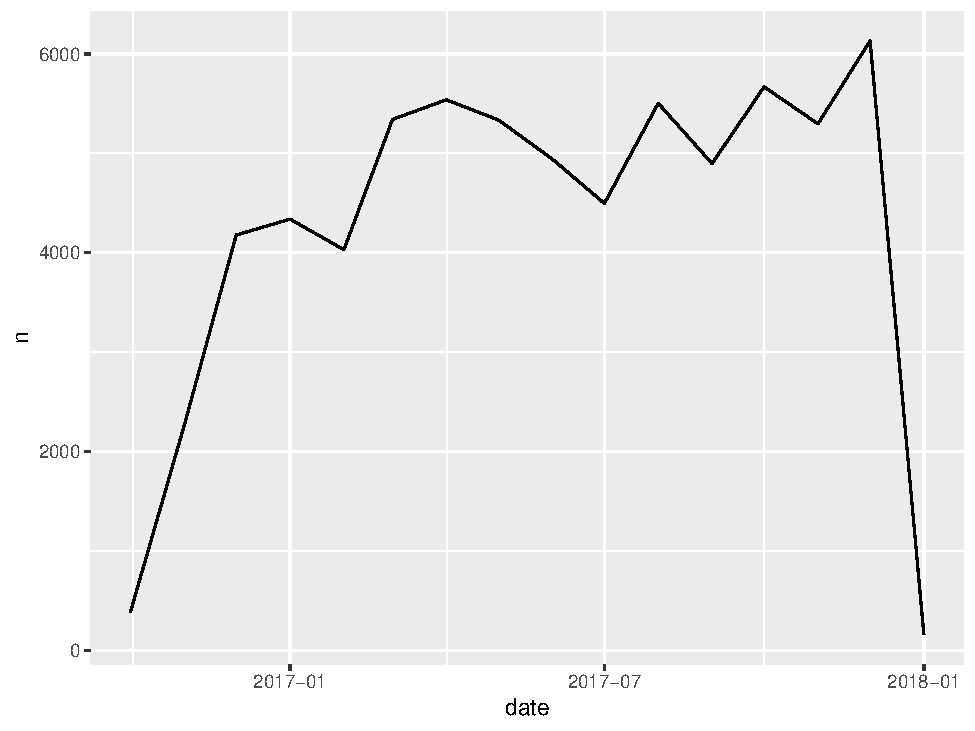
\includegraphics[width=0.9\linewidth]{bookdown-demo_files/figure-latex/unnamed-chunk-209-1} \end{center}

This is pretty good as it is. The better way of doing it is by storing the whole thing in a variable first and then calling that variable. That gives you more flexibility, for example, if you want to later do something to that plot. I will show you later what kind of things you can do to a plot stored in a variable. Lets store it first.

\begin{Shaded}
\begin{Highlighting}[]
\CommentTok{# Storing the plot.}
\NormalTok{ourLinePlot <-}\StringTok{ }\KeywordTok{ggplot}\NormalTok{(dataForLine, }\KeywordTok{aes}\NormalTok{(date, n)) }\OperatorTok{+}
\StringTok{  }\KeywordTok{geom_line}\NormalTok{()}
\end{Highlighting}
\end{Shaded}

Now that our line plot is stored in the variable `ourLinePlot', to show it, we need to just call the variable like this:

\begin{Shaded}
\begin{Highlighting}[]
\CommentTok{# Rendering.}
\NormalTok{ourLinePlot}
\end{Highlighting}
\end{Shaded}

\begin{center}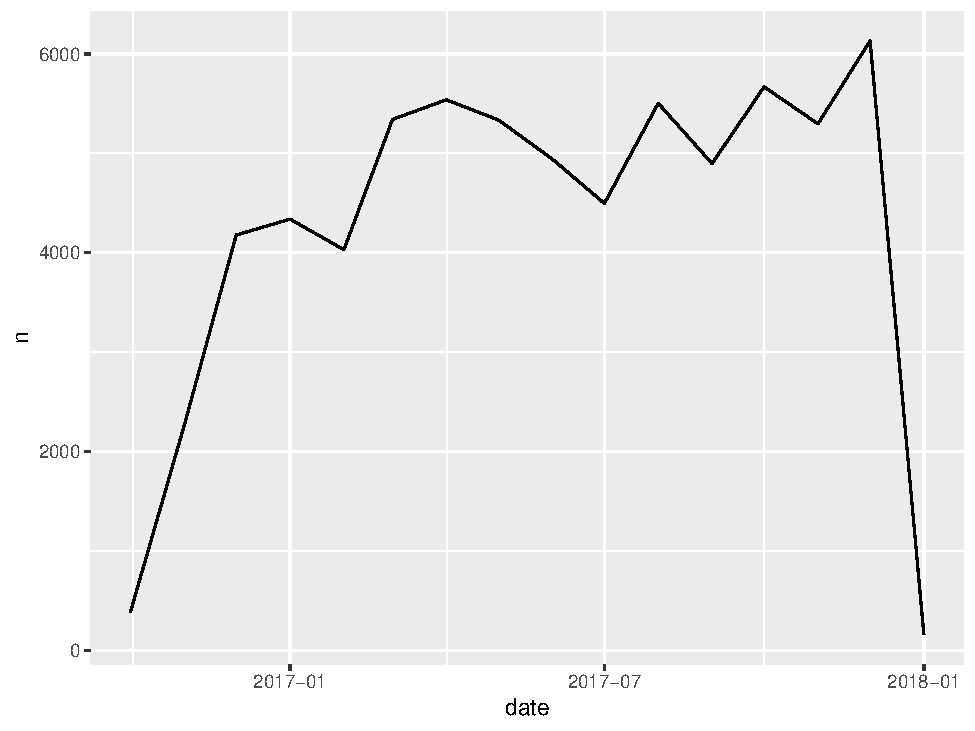
\includegraphics[width=0.9\linewidth]{bookdown-demo_files/figure-latex/unnamed-chunk-211-1} \end{center}

As you can see, storing and calling a plot from a variable produces the same result as just calling the ggplot() function straigh away. Lets see if we can layer a few things on top of our chart to make it look better. I want to add a title and change the color to red and make the line wider. Lets do it.

\begin{Shaded}
\begin{Highlighting}[]
\NormalTok{ourLinePlot <-}\StringTok{ }\KeywordTok{ggplot}\NormalTok{(dataForLine, }\KeywordTok{aes}\NormalTok{(date, n)) }\OperatorTok{+}
\StringTok{  }\CommentTok{# Adding size and color params to the line}
\StringTok{  }\KeywordTok{geom_line}\NormalTok{(}\DataTypeTok{size =} \FloatTok{1.5}\NormalTok{, }\DataTypeTok{color =} \StringTok{'red'}\NormalTok{) }\OperatorTok{+}
\StringTok{  }\CommentTok{# 'labs' can add a title and rename the x and y labels}
\StringTok{  }\KeywordTok{labs}\NormalTok{(}\DataTypeTok{title=}\StringTok{"Incoming Cars (by month)"}\NormalTok{)}

\NormalTok{ourLinePlot}
\end{Highlighting}
\end{Shaded}

\begin{center}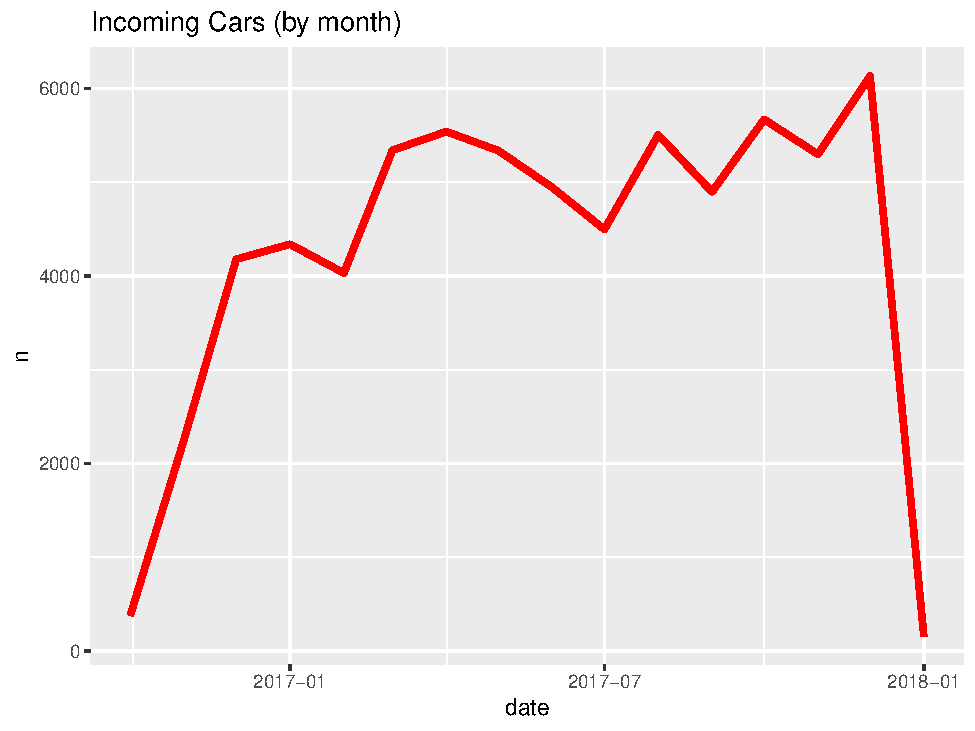
\includegraphics[width=0.9\linewidth]{bookdown-demo_files/figure-latex/unnamed-chunk-212-1} \end{center}

This is nicer. Y aixis says `n' and we only see three dates. That just looks weird. Lets change the x and y labels and make the x axis show us every month break instead of just three. Also, I want to change the date format to something like this: `2020-Jan'.

\begin{Shaded}
\begin{Highlighting}[]
\NormalTok{ourLinePlot <-}\StringTok{ }\KeywordTok{ggplot}\NormalTok{(dataForLine, }\KeywordTok{aes}\NormalTok{(date, n)) }\OperatorTok{+}
\StringTok{  }\KeywordTok{geom_line}\NormalTok{(}\DataTypeTok{size =} \FloatTok{1.5}\NormalTok{, }\DataTypeTok{color =} \StringTok{'red'}\NormalTok{) }\OperatorTok{+}
\StringTok{  }\CommentTok{# 'labs' can add a title and rename the x and y labels}
\StringTok{  }\KeywordTok{labs}\NormalTok{(}\DataTypeTok{title=}\StringTok{"Incoming Cars (by month)"}\NormalTok{, }\DataTypeTok{x=}\StringTok{"Date (month)"}\NormalTok{, }\DataTypeTok{y=}\StringTok{"New Cars"}\NormalTok{) }\OperatorTok{+}
\StringTok{  }\CommentTok{# the scale+x_date() lets us work with the x axis more closely.}
\StringTok{  }\CommentTok{# We can change the date format, and specify the breaks. We }
\StringTok{  }\CommentTok{# can also specify the date borders. I will show you that later.}
\StringTok{  }\KeywordTok{scale_x_date}\NormalTok{(}\DataTypeTok{labels =} \KeywordTok{date_format}\NormalTok{(}\StringTok{"%Y-%b"}\NormalTok{), }
               \DataTypeTok{breaks =} \KeywordTok{date_breaks}\NormalTok{(}\StringTok{"1 months"}\NormalTok{))}

\NormalTok{ourLinePlot}
\end{Highlighting}
\end{Shaded}

\begin{center}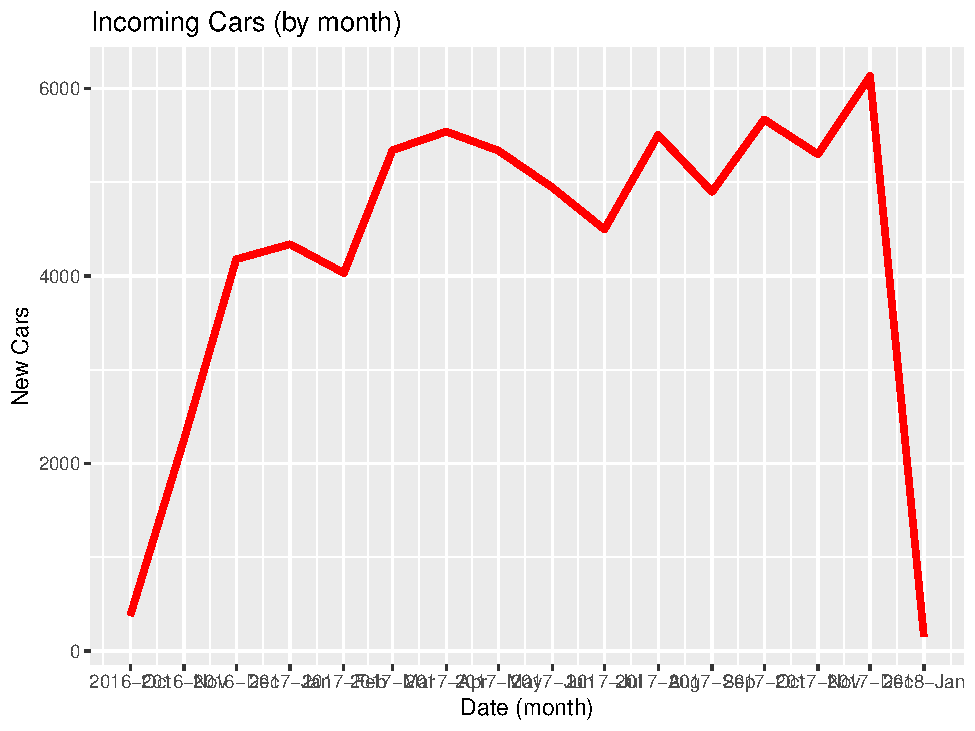
\includegraphics[width=1\linewidth]{bookdown-demo_files/figure-latex/unnamed-chunk-213-1} \end{center}

We are close. The first thing we need to fix is overlapping dates. We can tilt them 45 degrees and they should look better. The second thing I do not like is that ugly backgroud. We can apply one of the themes from the package ggthemes.

\begin{Shaded}
\begin{Highlighting}[]
\NormalTok{ourLinePlot <-}\StringTok{ }\KeywordTok{ggplot}\NormalTok{(dataForLine, }\KeywordTok{aes}\NormalTok{(date, n)) }\OperatorTok{+}
\StringTok{  }\KeywordTok{geom_line}\NormalTok{(}\DataTypeTok{size =} \FloatTok{1.5}\NormalTok{, }\DataTypeTok{color =} \StringTok{'red'}\NormalTok{) }\OperatorTok{+}
\StringTok{  }\KeywordTok{labs}\NormalTok{(}\DataTypeTok{title=}\StringTok{"Incoming Cars (by month)"}\NormalTok{, }
       \DataTypeTok{x=}\StringTok{"Date (month)"}\NormalTok{, }\DataTypeTok{y=}\StringTok{"New Cars"}\NormalTok{) }\OperatorTok{+}
\StringTok{  }\KeywordTok{scale_x_date}\NormalTok{(}\DataTypeTok{labels =} \KeywordTok{date_format}\NormalTok{(}\StringTok{"%Y-%b"}\NormalTok{), }
               \DataTypeTok{breaks =} \KeywordTok{date_breaks}\NormalTok{(}\StringTok{"1 months"}\NormalTok{)) }\OperatorTok{+}
\StringTok{  }\CommentTok{# The function theme() lets us move the text around. }
\StringTok{  }\KeywordTok{theme}\NormalTok{(}\DataTypeTok{axis.text.x =} \KeywordTok{element_text}\NormalTok{(}\DataTypeTok{angle =} \DecValTok{45}\NormalTok{)) }\OperatorTok{+}
\StringTok{  }\CommentTok{# The function below is the ggthemes function. You should check}
\StringTok{  }\CommentTok{# out their themes. We are using the 'hc'}
\StringTok{  }\KeywordTok{theme_hc}\NormalTok{()}

\NormalTok{ourLinePlot}
\end{Highlighting}
\end{Shaded}

\begin{center}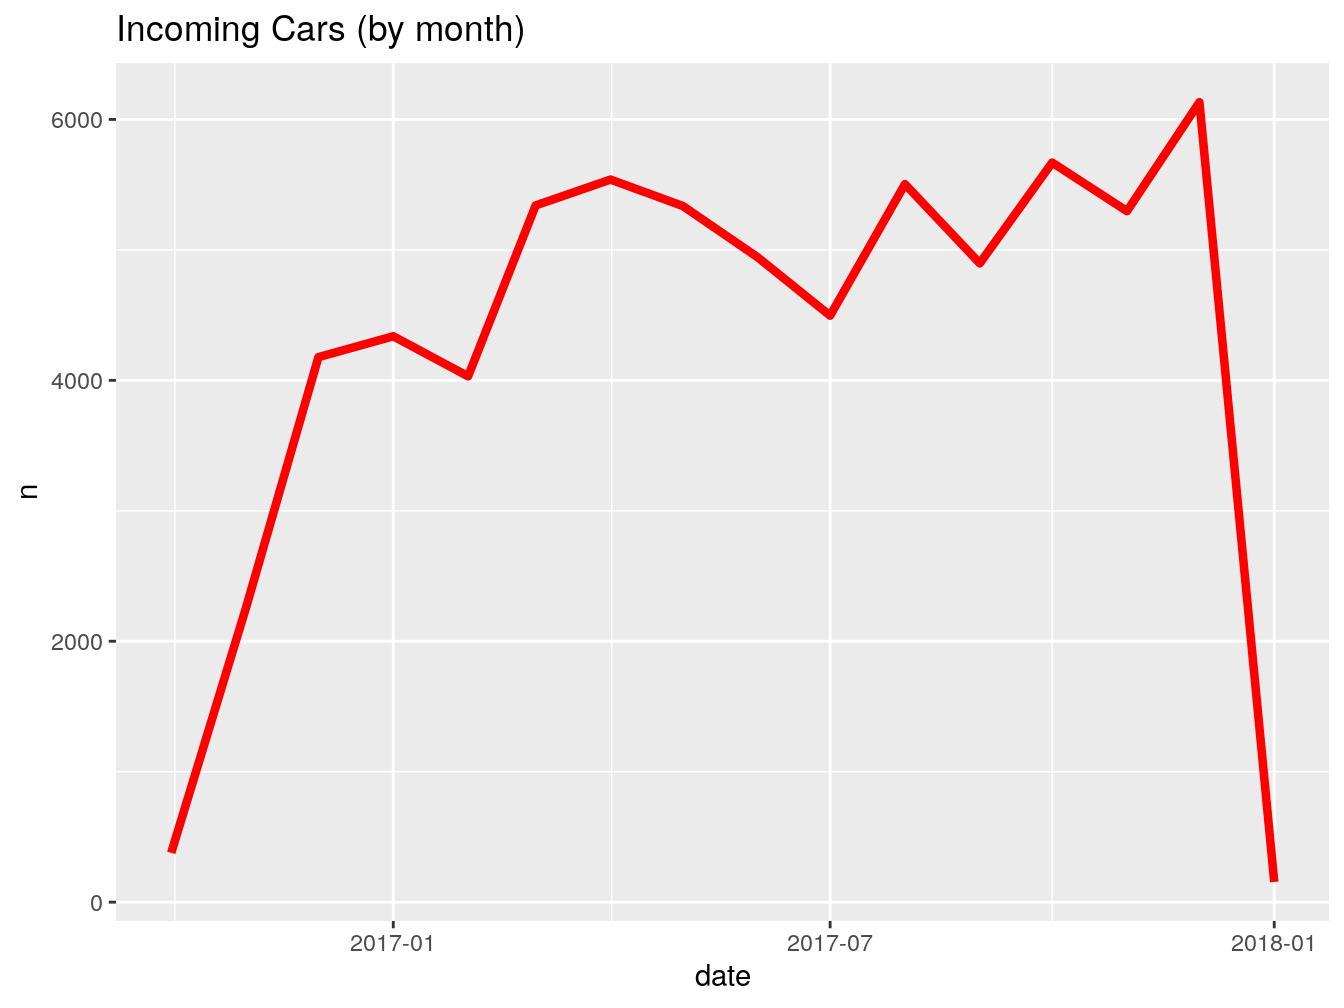
\includegraphics[width=1\linewidth]{bookdown-demo_files/figure-latex/unnamed-chunk-214-1} \end{center}

This looks really nice. There are two last things that I want to change before we move on though. The date labels are a bit too high and the first and the last data points are outliers that we should get rid of (just not good from the presentation standpoint). The first we can remedy by adding the hjust input into the theme() function. The second, by adding the limits into the scale\_x\_date() function.

\begin{Shaded}
\begin{Highlighting}[]
\NormalTok{ourLinePlot <-}\StringTok{ }\KeywordTok{ggplot}\NormalTok{(dataForLine, }\KeywordTok{aes}\NormalTok{(date, n)) }\OperatorTok{+}
\StringTok{  }\KeywordTok{geom_line}\NormalTok{(}\DataTypeTok{size =} \FloatTok{1.5}\NormalTok{, }\DataTypeTok{color =} \StringTok{'red'}\NormalTok{) }\OperatorTok{+}
\StringTok{  }\KeywordTok{labs}\NormalTok{(}\DataTypeTok{title=}\StringTok{"Incoming Cars (by month)"}\NormalTok{, }
       \DataTypeTok{x=}\StringTok{"Date (month)"}\NormalTok{, }\DataTypeTok{y=}\StringTok{"New Cars"}\NormalTok{) }\OperatorTok{+}
\StringTok{  }\KeywordTok{scale_x_date}\NormalTok{(}\DataTypeTok{labels =} \KeywordTok{date_format}\NormalTok{(}\StringTok{"%Y-%b"}\NormalTok{), }
               \DataTypeTok{breaks =} \KeywordTok{date_breaks}\NormalTok{(}\StringTok{"1 months"}\NormalTok{), }
               \DataTypeTok{limits =} \KeywordTok{as.Date}\NormalTok{(}\KeywordTok{c}\NormalTok{(}\StringTok{'2016-12-01'}\NormalTok{,}\StringTok{'2017-12-01'}\NormalTok{))) }\OperatorTok{+}
\StringTok{  }\CommentTok{# The hjust = 1 will move the tick labels down just enough.}
\StringTok{  }\CommentTok{# You should definitely play with some of these params}
\StringTok{  }\KeywordTok{theme}\NormalTok{(}\DataTypeTok{axis.text.x =} \KeywordTok{element_text}\NormalTok{(}\DataTypeTok{angle =} \DecValTok{45}\NormalTok{, }\DataTypeTok{hjust =} \DecValTok{1}\NormalTok{)) }\OperatorTok{+}
\StringTok{  }\KeywordTok{theme_hc}\NormalTok{()}

\NormalTok{ourLinePlot}
\end{Highlighting}
\end{Shaded}

\begin{verbatim}
## Warning: Removed 3 rows containing missing values (geom_path).
\end{verbatim}

\begin{center}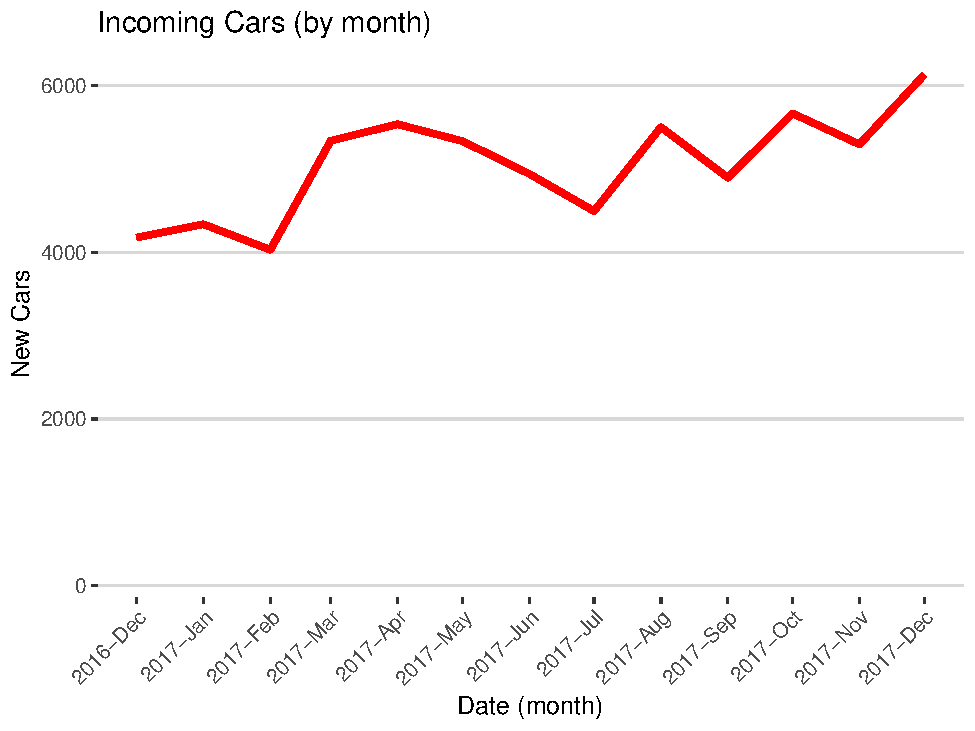
\includegraphics[width=1\linewidth]{bookdown-demo_files/figure-latex/unnamed-chunk-215-1} \end{center}

We are done here. This looks very professional now. One thing to change here would be the scale of the y axis. See if you can change it to 2000 to 7000 by yourself. That will be a good practice for you. If you look at the final code that we have you will see that it was not hard at all. It might be a bit time consumng at the beginning, because you have to get just the right balance for your plot. You might be wondering why am I not going deep into each parameter of every function anymore. First of all, this topic and the next few are quite big and deserve books of their own. In fact, they do have books of their own. Secondly, by now you should be able to understand how functions and parameters of those functions work, at least on a basic level. At this point, I just want to show you how the things can and should look and how to achive that. You should be able to look deeper into them and tweak them on your own. You should be able to chew your own food from now on. I am still feeding you from a spoon though.

For the rest of this section, I want to show you different ways we can plot our data. Lets see whay our line plot would look like if we had a grouping variable there. Lets add the fuel type as a grouping varible. The data aggregation for that will be very similar to what we did for the basic line plot. The extra stuff that we need to do here is selecting the gas1 and gas2 and renaming them just line we did when we were creating our unique identifier. We will just copy it from there.

\begin{Shaded}
\begin{Highlighting}[]
\CommentTok{# Selecting the columns.}
\NormalTok{dataForFuelLine <-}\StringTok{ }\NormalTok{data }\OperatorTok\StringTok{ }
\StringTok{  }\NormalTok{dplyr}\OperatorTok{::}\KeywordTok{select}\NormalTok{(vin, date, gas1, gas2)}
\CommentTok{# Renaming empty spaces into nas.}
\NormalTok{dataForFuelLine <-}\StringTok{ }\NormalTok{dataForFuelLine[gas2 }\OperatorTok{==}\StringTok{ ''}\NormalTok{, gas2}\OperatorTok{:}\ErrorTok{=}\OtherTok{NA}\NormalTok{]}
\NormalTok{dataForFuelLine <-}\StringTok{ }\NormalTok{dataForFuelLine[gas1 }\OperatorTok{==}\StringTok{ ''}\NormalTok{, gas1}\OperatorTok{:}\ErrorTok{=}\OtherTok{NA}\NormalTok{]}

\CommentTok{# Conditionally abbriviating the fuel types.}
\NormalTok{dataForFuelLine <-}\StringTok{ }
\StringTok{  }\KeywordTok{setDT}\NormalTok{(dataForFuelLine)[dataForFuelLine}\OperatorTok{$}\NormalTok{gas1 }\OperatorTok{==}\StringTok{ }
\StringTok{                           'Gasoline'} \OperatorTok{&}\StringTok{ }
\StringTok{                                }\KeywordTok{is.na}\NormalTok{(dataForFuelLine}\OperatorTok{$}\NormalTok{gas2),Type}\OperatorTok{:}\ErrorTok{=}\StringTok{'g'}\NormalTok{]}

\NormalTok{dataForFuelLine <-}\StringTok{ }
\StringTok{  }\KeywordTok{setDT}\NormalTok{(dataForFuelLine)[dataForFuelLine}\OperatorTok{$}\NormalTok{gas1 }\OperatorTok{==}\StringTok{ }
\StringTok{                           'Gasoline'} \OperatorTok{&}\StringTok{ }
\StringTok{                               }\NormalTok{dataForFuelLine}\OperatorTok{$}\NormalTok{gas2 }\OperatorTok{==}\StringTok{ }
\StringTok{                           'Electric'}\NormalTok{,Type}\OperatorTok{:}\ErrorTok{=}\StringTok{'h'}\NormalTok{]}

\NormalTok{dataForFuelLine <-}\StringTok{ }
\StringTok{  }\KeywordTok{setDT}\NormalTok{(dataForFuelLine)[dataForFuelLine}\OperatorTok{$}\NormalTok{gas1 }\OperatorTok{==}\StringTok{ }
\StringTok{                           'Gasoline'} \OperatorTok{&}\StringTok{ }
\StringTok{                                }\NormalTok{dataForFuelLine}\OperatorTok{$}\NormalTok{gas2 }\OperatorTok{==}\StringTok{ }
\StringTok{                           'Ethanol (E85)'}\NormalTok{,Type}\OperatorTok{:}\ErrorTok{=}\StringTok{'h'}\NormalTok{]}

\NormalTok{dataForFuelLine <-}\StringTok{ }
\StringTok{  }\KeywordTok{setDT}\NormalTok{(dataForFuelLine)[}\KeywordTok{is.na}\NormalTok{(dataForFuelLine}\OperatorTok{$}\NormalTok{gas1) }\OperatorTok{&}\StringTok{ }
\StringTok{                                }\KeywordTok{is.na}\NormalTok{(dataForFuelLine}\OperatorTok{$}\NormalTok{gas2),Type}\OperatorTok{:}\ErrorTok{=}\StringTok{'Unknown'}\NormalTok{]}

\NormalTok{dataForFuelLine <-}\StringTok{ }
\StringTok{  }\KeywordTok{setDT}\NormalTok{(dataForFuelLine)[dataForFuelLine}\OperatorTok{$}\NormalTok{gas1 }\OperatorTok{==}\StringTok{ }
\StringTok{                           'Flexible Fuel Vehicle (FFV)'} \OperatorTok{&}\StringTok{ }
\StringTok{                                }\NormalTok{dataForFuelLine}\OperatorTok{$}\NormalTok{gas2 }\OperatorTok{==}\StringTok{ }
\StringTok{                           'Gasoline'}\NormalTok{,Type}\OperatorTok{:}\ErrorTok{=}\StringTok{'h'}\NormalTok{]}

\NormalTok{dataForFuelLine <-}\StringTok{ }
\StringTok{  }\KeywordTok{setDT}\NormalTok{(dataForFuelLine)[dataForFuelLine}\OperatorTok{$}\NormalTok{gas1 }\OperatorTok{==}\StringTok{ }
\StringTok{                           'Flexible Fuel Vehicle (FFV)'} \OperatorTok{&}
\StringTok{                                }\KeywordTok{is.na}\NormalTok{(dataForFuelLine}\OperatorTok{$}\NormalTok{gas2),Type}\OperatorTok{:}\ErrorTok{=}\StringTok{'h'}\NormalTok{]}

\NormalTok{dataForFuelLine <-}
\StringTok{  }\KeywordTok{setDT}\NormalTok{(dataForFuelLine)[dataForFuelLine}\OperatorTok{$}\NormalTok{gas1 }\OperatorTok{==}\StringTok{ }
\StringTok{                           'Electric'} \OperatorTok{&}\StringTok{ }
\StringTok{                                }\NormalTok{dataForFuelLine}\OperatorTok{$}\NormalTok{gas2 }\OperatorTok{==}\StringTok{ }
\StringTok{                           'Gasoline'}\NormalTok{,Type}\OperatorTok{:}\ErrorTok{=}\StringTok{'h'}\NormalTok{]}

\NormalTok{dataForFuelLine <-}\StringTok{ }
\StringTok{  }\KeywordTok{setDT}\NormalTok{(dataForFuelLine)[dataForFuelLine}\OperatorTok{$}\NormalTok{gas1 }\OperatorTok{==}\StringTok{ }
\StringTok{                           'Diesel'} \OperatorTok{&}\StringTok{ }
\StringTok{                                }\KeywordTok{is.na}\NormalTok{(dataForFuelLine}\OperatorTok{$}\NormalTok{gas2),Type}\OperatorTok{:}\ErrorTok{=}\StringTok{'d'}\NormalTok{]}

\NormalTok{dataForFuelLine <-}\StringTok{ }
\StringTok{  }\KeywordTok{setDT}\NormalTok{(dataForFuelLine)[dataForFuelLine}\OperatorTok{$}\NormalTok{gas1 }\OperatorTok{==}\StringTok{ }
\StringTok{                           'Gasoline'} \OperatorTok{&}\StringTok{ }
\StringTok{                                }\NormalTok{dataForFuelLine}\OperatorTok{$}\NormalTok{gas2 }\OperatorTok{==}\StringTok{ }
\StringTok{                           'Flexible Fuel Vehicle (FFV)'}\NormalTok{,Type}\OperatorTok{:}\ErrorTok{=}\StringTok{'h'}\NormalTok{]}

\NormalTok{dataForFuelLine <-}\StringTok{ }
\StringTok{  }\KeywordTok{setDT}\NormalTok{(dataForFuelLine)[dataForFuelLine}\OperatorTok{$}\NormalTok{gas1 }\OperatorTok{==}\StringTok{ }
\StringTok{                           'Flexible Fuel Vehicle (FFV), Gasoline'} \OperatorTok{&}
\StringTok{                                }\NormalTok{dataForFuelLine}\OperatorTok{$}\NormalTok{gas2 }\OperatorTok{==}\StringTok{ }
\StringTok{                           'Ethanol (E85)'}\NormalTok{,Type}\OperatorTok{:}\ErrorTok{=}\StringTok{'h'}\NormalTok{]}

\NormalTok{dataForFuelLine <-}\StringTok{ }
\StringTok{  }\KeywordTok{setDT}\NormalTok{(dataForFuelLine)[dataForFuelLine}\OperatorTok{$}\NormalTok{gas1 }\OperatorTok{==}\StringTok{ }
\StringTok{                           'Gasoline, Flexible Fuel Vehicle (FFV)'} \OperatorTok{&}
\StringTok{                               }\NormalTok{dataForFuelLine}\OperatorTok{$}\NormalTok{gas2 }\OperatorTok{==}\StringTok{ }
\StringTok{                           'Ethanol (E85)'}\NormalTok{,Type}\OperatorTok{:}\ErrorTok{=}\StringTok{'h'}\NormalTok{]}

\NormalTok{dataForFuelLine <-}\StringTok{ }
\StringTok{  }\KeywordTok{setDT}\NormalTok{(dataForFuelLine)[dataForFuelLine}\OperatorTok{$}\NormalTok{gas1 }\OperatorTok{==}\StringTok{ }
\StringTok{                           'Electric'} \OperatorTok{&}\StringTok{ }
\StringTok{                                }\KeywordTok{is.na}\NormalTok{(dataForFuelLine}\OperatorTok{$}\NormalTok{gas2),Type}\OperatorTok{:}\ErrorTok{=}\StringTok{'e'}\NormalTok{]}

\NormalTok{dataForFuelLine <-}\StringTok{ }
\StringTok{  }\KeywordTok{setDT}\NormalTok{(dataForFuelLine)[dataForFuelLine}\OperatorTok{$}\NormalTok{gas1 }\OperatorTok{==}\StringTok{ }
\StringTok{                           'Gasoline, Electric'} \OperatorTok{&}\StringTok{ }
\StringTok{                                }\NormalTok{dataForFuelLine}\OperatorTok{$}\NormalTok{gas2 }\OperatorTok{==}\StringTok{ }
\StringTok{                           'Electric, Gasoline'}\NormalTok{,Type}\OperatorTok{:}\ErrorTok{=}\StringTok{'h'}\NormalTok{]}

\NormalTok{dataForFuelLine <-}\StringTok{ }
\StringTok{  }\KeywordTok{setDT}\NormalTok{(dataForFuelLine)[dataForFuelLine}\OperatorTok{$}\NormalTok{gas1 }\OperatorTok{==}\StringTok{ }
\StringTok{                           'Gasoline'} \OperatorTok{&}\StringTok{ }
\StringTok{                                }\NormalTok{dataForFuelLine}\OperatorTok{$}\NormalTok{gas2 }\OperatorTok{==}\StringTok{ }
\StringTok{                           'Compressed Natural Gas (CNG)'}\NormalTok{,Type}\OperatorTok{:}\ErrorTok{=}\StringTok{'h'}\NormalTok{]}

\NormalTok{dataForFuelLine <-}\StringTok{ }
\StringTok{  }\KeywordTok{setDT}\NormalTok{(dataForFuelLine)[dataForFuelLine}\OperatorTok{$}\NormalTok{gas1 }\OperatorTok{==}\StringTok{ }
\StringTok{                           'Electric, Gasoline'} \OperatorTok{&}\StringTok{ }
\StringTok{                                }\NormalTok{dataForFuelLine}\OperatorTok{$}\NormalTok{gas2 }\OperatorTok{==}\StringTok{ }
\StringTok{                           'Gasoline, Electric'}\NormalTok{,Type}\OperatorTok{:}\ErrorTok{=}\StringTok{'h'}\NormalTok{]}

\NormalTok{dataForFuelLine <-}\StringTok{ }
\StringTok{  }\KeywordTok{setDT}\NormalTok{(dataForFuelLine)[dataForFuelLine}\OperatorTok{$}\NormalTok{gas1 }\OperatorTok{==}\StringTok{ }
\StringTok{                           'Gasoline, Flexible Fuel Vehicle (FFV)'} \OperatorTok{&}
\StringTok{                                }\NormalTok{dataForFuelLine}\OperatorTok{$}\NormalTok{gas2 }\OperatorTok{==}\StringTok{ }
\StringTok{                           'Gasoline'}\NormalTok{,Type}\OperatorTok{:}\ErrorTok{=}\StringTok{'h'}\NormalTok{]}

\NormalTok{dataForFuelLine <-}\StringTok{ }
\StringTok{  }\KeywordTok{setDT}\NormalTok{(dataForFuelLine)[}\KeywordTok{is.na}\NormalTok{(dataForFuelLine}\OperatorTok{$}\NormalTok{gas1) }\OperatorTok{&}\StringTok{ }
\StringTok{                                }\NormalTok{dataForFuelLine}\OperatorTok{$}\NormalTok{gas2 }\OperatorTok{==}\StringTok{ }
\StringTok{                           'Gasoline'}\NormalTok{,Type}\OperatorTok{:}\ErrorTok{=}\StringTok{'g'}\NormalTok{]}

\NormalTok{dataForFuelLine <-}\StringTok{ }
\StringTok{  }\KeywordTok{setDT}\NormalTok{(dataForFuelLine)[dataForFuelLine}\OperatorTok{$}\NormalTok{gas1 }\OperatorTok{==}\StringTok{ }
\StringTok{                           'Compressed Natural Gas (CNG)'} \OperatorTok{&}
\StringTok{                                }\KeywordTok{is.na}\NormalTok{(dataForFuelLine}\OperatorTok{$}\NormalTok{gas2),Type}\OperatorTok{:}\ErrorTok{=}\StringTok{'cng'}\NormalTok{]}

\NormalTok{dataForFuelLine <-}\StringTok{ }
\StringTok{  }\KeywordTok{setDT}\NormalTok{(dataForFuelLine)[dataForFuelLine}\OperatorTok{$}\NormalTok{gas1 }\OperatorTok{==}\StringTok{ }
\StringTok{                           'Ethanol (E85)'} \OperatorTok{&}
\StringTok{                                }\KeywordTok{is.na}\NormalTok{(dataForFuelLine}\OperatorTok{$}\NormalTok{gas2),Type}\OperatorTok{:}\ErrorTok{=}\StringTok{'ethnl'}\NormalTok{]}

\NormalTok{dataForFuelLine <-}\StringTok{ }
\StringTok{  }\KeywordTok{setDT}\NormalTok{(dataForFuelLine)[dataForFuelLine}\OperatorTok{$}\NormalTok{gas1 }\OperatorTok{==}\StringTok{ }
\StringTok{                           'Flexible Fuel Vehicle (FFV)'} \OperatorTok{&}\StringTok{ }
\StringTok{                                }\NormalTok{dataForFuelLine}\OperatorTok{$}\NormalTok{gas2 }\OperatorTok{==}\StringTok{ }
\StringTok{                           'Electric'}\NormalTok{,Type}\OperatorTok{:}\ErrorTok{=}\StringTok{'h'}\NormalTok{]}

\NormalTok{dataForFuelLine <-}\StringTok{ }
\StringTok{  }\KeywordTok{setDT}\NormalTok{(dataForFuelLine)[dataForFuelLine}\OperatorTok{$}\NormalTok{gas1 }\OperatorTok{==}\StringTok{ }
\StringTok{                           'Flexible Fuel Vehicle (FFV), Gasoline'} \OperatorTok{&}
\StringTok{                                }\NormalTok{dataForFuelLine}\OperatorTok{$}\NormalTok{gas2 }\OperatorTok{==}\StringTok{ }
\StringTok{                           'Gasoline'}\NormalTok{,Type}\OperatorTok{:}\ErrorTok{=}\StringTok{'h'}\NormalTok{]}

\NormalTok{dataForFuelLine <-}\StringTok{ }
\StringTok{  }\KeywordTok{setDT}\NormalTok{(dataForFuelLine)[dataForFuelLine}\OperatorTok{$}\NormalTok{gas1 }\OperatorTok{==}\StringTok{ }
\StringTok{                           'Electric, Gasoline'} \OperatorTok{&}
\StringTok{                                }\KeywordTok{is.na}\NormalTok{(dataForFuelLine}\OperatorTok{$}\NormalTok{gas2),Type}\OperatorTok{:}\ErrorTok{=}\StringTok{'h'}\NormalTok{]}

\NormalTok{dataForFuelLine <-}\StringTok{ }
\StringTok{  }\KeywordTok{setDT}\NormalTok{(dataForFuelLine)[dataForFuelLine}\OperatorTok{$}\NormalTok{gas1 }\OperatorTok{==}\StringTok{ }
\StringTok{                           'Liquefied Petroleum Gas (propane or LPG)'} \OperatorTok{&}
\StringTok{                                }\KeywordTok{is.na}\NormalTok{(dataForFuelLine}\OperatorTok{$}\NormalTok{gas2),Type}\OperatorTok{:}\ErrorTok{=}\StringTok{'lpg'}\NormalTok{]}
\end{Highlighting}
\end{Shaded}

We are interested in seeing how many vehicles came in every month, by fuel type this time. We will do here exactly what we did for the first line plot, plus add the `Type' as another grouping variable.

Converting the date column from character to date format.

\begin{Shaded}
\begin{Highlighting}[]
\CommentTok{# Converting.}
\NormalTok{dataForFuelLine}\OperatorTok{$}\NormalTok{date <-}\StringTok{ }\NormalTok{lubridate}\OperatorTok{::}\KeywordTok{ymd}\NormalTok{(dataForFuelLine}\OperatorTok{$}\NormalTok{date)}
\end{Highlighting}
\end{Shaded}

Flooring to a month.

\begin{Shaded}
\begin{Highlighting}[]
\CommentTok{# Flooring.}
\NormalTok{dataForFuelLine}\OperatorTok{$}\NormalTok{date <-}\StringTok{ }\NormalTok{lubridate}\OperatorTok{::}\KeywordTok{floor_date}\NormalTok{(dataForFuelLine}\OperatorTok{$}\NormalTok{date, }\StringTok{'month'}\NormalTok{)}
\end{Highlighting}
\end{Shaded}

Calculating.

\begin{Shaded}
\begin{Highlighting}[]
\CommentTok{# Grouping and counting.}
\NormalTok{dataForFuelLine <-}\StringTok{ }\NormalTok{dataForFuelLine }\OperatorTok\StringTok{ }
\NormalTok{dplyr}\OperatorTok{::}\KeywordTok{group_by}\NormalTok{(date, Type) }\OperatorTok\StringTok{ }
\NormalTok{dplyr}\OperatorTok{::}\KeywordTok{count}\NormalTok{()}
\end{Highlighting}
\end{Shaded}

Lets see what it looks like.

\begin{Shaded}
\begin{Highlighting}[]
\CommentTok{# Printing.}
\KeywordTok{print}\NormalTok{(}\KeywordTok{head}\NormalTok{(dataForFuelLine))}
\end{Highlighting}
\end{Shaded}

\begin{verbatim}
## # A tibble: 6 x 3
## # Groups:   date, Type [6]
##   date       Type        n
##   <date>     <chr>   <int>
## 1 2016-10-01 g         278
## 2 2016-10-01 h          76
## 3 2016-10-01 Unknown    24
## 4 2016-11-01 d           5
## 5 2016-11-01 g        1701
## 6 2016-11-01 h         439
\end{verbatim}

Perfect. We aggregated the data just the way we needed. Lets take the final plot code and see how it the plot changes when we add fuel as the grouping variable.

We need to add the `color' input. It will serve as a grouping parameter.

\begin{Shaded}
\begin{Highlighting}[]
\CommentTok{# Plot.}
\NormalTok{ourLineFuelPlot <-}\StringTok{ }\KeywordTok{ggplot}\NormalTok{(dataForFuelLine, }\KeywordTok{aes}\NormalTok{(date, n, }\DataTypeTok{color =}\NormalTok{ Type)) }\OperatorTok{+}
\StringTok{  }\CommentTok{# We need to eliminate the color parameter from the geom_line(), }
\StringTok{  }\CommentTok{# because we already specified it in the aes() above.}
\StringTok{  }\KeywordTok{geom_line}\NormalTok{(}\DataTypeTok{size =} \FloatTok{1.5}\NormalTok{) }\OperatorTok{+}
\StringTok{  }\KeywordTok{labs}\NormalTok{(}\DataTypeTok{title=}\StringTok{"Incoming Cars (by fuel type)"}\NormalTok{, }
       \DataTypeTok{x=}\StringTok{"Date (month)"}\NormalTok{, }\DataTypeTok{y=}\StringTok{"New Cars"}\NormalTok{) }\OperatorTok{+}
\StringTok{  }\KeywordTok{scale_x_date}\NormalTok{(}\DataTypeTok{labels =} \KeywordTok{date_format}\NormalTok{(}\StringTok{"%Y-%b"}\NormalTok{), }
               \DataTypeTok{breaks =} \KeywordTok{date_breaks}\NormalTok{(}\StringTok{"1 months"}\NormalTok{), }
               \DataTypeTok{limits =} \KeywordTok{as.Date}\NormalTok{(}\KeywordTok{c}\NormalTok{(}\StringTok{'2016-12-01'}\NormalTok{,}\StringTok{'2017-12-01'}\NormalTok{))) }\OperatorTok{+}
\StringTok{  }\KeywordTok{theme}\NormalTok{(}\DataTypeTok{axis.text.x =} \KeywordTok{element_text}\NormalTok{(}\DataTypeTok{angle =} \DecValTok{45}\NormalTok{, }\DataTypeTok{hjust =} \DecValTok{1}\NormalTok{)) }\OperatorTok{+}
\StringTok{  }\KeywordTok{theme_hc}\NormalTok{()}

\NormalTok{ourLineFuelPlot}
\end{Highlighting}
\end{Shaded}

\begin{center}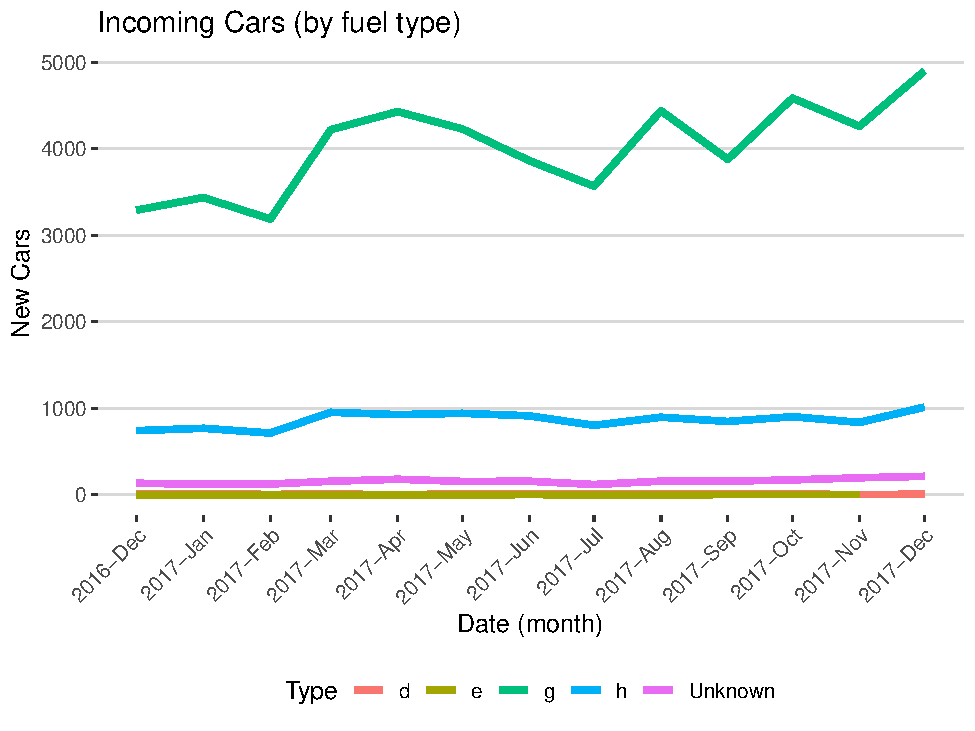
\includegraphics[width=1\linewidth]{bookdown-demo_files/figure-latex/unnamed-chunk-221-1} \end{center}

We almost did not to do anything here. We basically, just recylced the same code we wrote before. We just tweaked two small things. This is what it is all about, get the code that works well for you and recycle it with some tweaking. I do not only mean plotting, but the same concept works across programming as a whole.

There is one thing I do not like about this plot though. The diesel (d) and electric (e) are on the bottom of the plot and there is no way to tell how many there actually are. There are a few ways to solve this problem. My favorite is to make this plot interactive. I will show you this way later. The second is to create multiple views where each view will represent a singel group. Lets do this now.

Again, we are just recycling the same code with minor tweaking.

\begin{Shaded}
\begin{Highlighting}[]
\CommentTok{# Plot.}
\NormalTok{ourLineFuelPlotFacet <-}\StringTok{ }\KeywordTok{ggplot}\NormalTok{(dataForFuelLine, }\KeywordTok{aes}\NormalTok{(date, n, }\DataTypeTok{color =}\NormalTok{ Type)) }\OperatorTok{+}
\StringTok{  }\KeywordTok{geom_line}\NormalTok{(}\DataTypeTok{size =} \FloatTok{1.5}\NormalTok{) }\OperatorTok{+}
\CommentTok{# The function facet_wrap() will split our plot into multiple plots}
\CommentTok{# by the specified parameter, which is our grouping parameter in this}
\CommentTok{# case.}
\StringTok{  }\KeywordTok{facet_wrap}\NormalTok{(}\OperatorTok{~}\NormalTok{Type) }\OperatorTok{+}
\StringTok{  }\KeywordTok{labs}\NormalTok{(}\DataTypeTok{title=}\StringTok{"Incoming Cars (by fuel type)"}\NormalTok{, }
       \DataTypeTok{x=}\StringTok{"Date (month)"}\NormalTok{, }\DataTypeTok{y=}\StringTok{"New Cars"}\NormalTok{) }\OperatorTok{+}
\CommentTok{# I suspect that '1 months' break will be too dense for small charts we }
\CommentTok{# are creating. Lets change it to '2 months'}
\StringTok{  }\KeywordTok{scale_x_date}\NormalTok{(}\DataTypeTok{labels =} \KeywordTok{date_format}\NormalTok{(}\StringTok{"%Y-%b"}\NormalTok{), }
               \DataTypeTok{breaks =} \KeywordTok{date_breaks}\NormalTok{(}\StringTok{"2 months"}\NormalTok{), }
               \DataTypeTok{limits =} \KeywordTok{as.Date}\NormalTok{(}\KeywordTok{c}\NormalTok{(}\StringTok{'2016-12-01'}\NormalTok{,}\StringTok{'2017-12-01'}\NormalTok{))) }\OperatorTok{+}
\StringTok{  }\KeywordTok{theme}\NormalTok{(}\DataTypeTok{axis.text.x =} \KeywordTok{element_text}\NormalTok{(}\DataTypeTok{angle =} \DecValTok{45}\NormalTok{, }\DataTypeTok{hjust =} \DecValTok{1}\NormalTok{)) }\OperatorTok{+}
\StringTok{  }\KeywordTok{theme_hc}\NormalTok{()}

\NormalTok{ourLineFuelPlotFacet}
\end{Highlighting}
\end{Shaded}

\begin{center}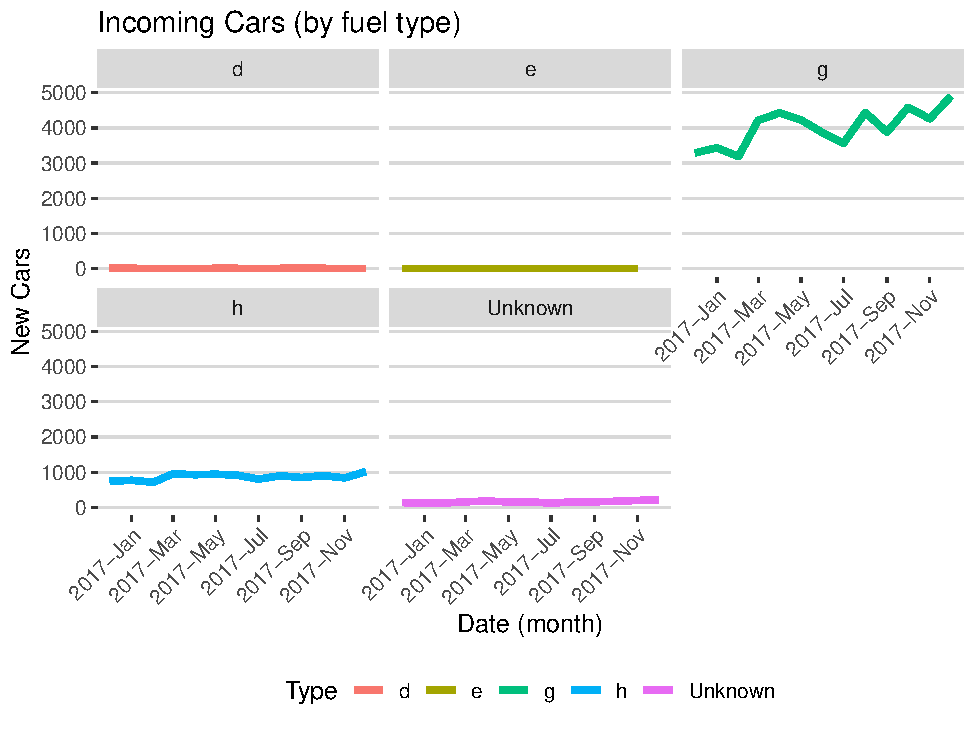
\includegraphics[width=1\linewidth]{bookdown-demo_files/figure-latex/unnamed-chunk-222-1} \end{center}

This did not really solve our problem. The scales are still the same and therefore d and e are still on the bottom. There are ways to fix it in ggplot() but I think I know a better way. Soon, we will be making these charts interactive and that will solve our issue. At least, you now know how to create a multiview with the facet\_wrap() function.

Before we do interactive charts, I want to show you my favorite type of plot, the bar plot. There will be not much different to what we have been doing so far. I like bar plots better, because I feel that they are just more informative. It is just a matter of preference.

Lets create a bar plot where we will demonstrate average ages of incoming vehicles by month. Similarly to the line plots, we first need to prepare the data.

First, we need to isolate the columns that we need.

\begin{Shaded}
\begin{Highlighting}[]
\CommentTok{# Selecting.}
\NormalTok{dataForBarPlot <-}\StringTok{ }\NormalTok{data }\OperatorTok\StringTok{ }
\StringTok{  }\NormalTok{dplyr}\OperatorTok{::}\KeywordTok{select}\NormalTok{(vin, date, year)}
\end{Highlighting}
\end{Shaded}

Lets calculte age of our vehicles. We are just deducting the year of a vehicle from the current year. Change `2020' to your year if it is different.

\begin{Shaded}
\begin{Highlighting}[]
\CommentTok{# Calculating ages.}
\NormalTok{dataForBarPlot}\OperatorTok{$}\NormalTok{year <-}\StringTok{ }\DecValTok{2020} \OperatorTok{-}\StringTok{ }\NormalTok{dataForBarPlot}\OperatorTok{$}\NormalTok{year}
\CommentTok{# Printing.}
\KeywordTok{print}\NormalTok{(}\KeywordTok{head}\NormalTok{(dataForBarPlot}\OperatorTok{$}\NormalTok{year))}
\end{Highlighting}
\end{Shaded}

\begin{verbatim}
## [1] 10  5 13  3  4  8
\end{verbatim}

Nice. We got the ages. Lets again floor our date column to a month.

\begin{Shaded}
\begin{Highlighting}[]
\CommentTok{# Flooring.}
\NormalTok{dataForBarPlot}\OperatorTok{$}\NormalTok{date <-}\StringTok{ }
\StringTok{  }\NormalTok{lubridate}\OperatorTok{::}\KeywordTok{floor_date}\NormalTok{(}\KeywordTok{ymd}\NormalTok{(dataForBarPlot}\OperatorTok{$}\NormalTok{date), }\StringTok{'months'}\NormalTok{)}
\end{Highlighting}
\end{Shaded}

Now, we can find the average age of our vehicles by month.

\begin{Shaded}
\begin{Highlighting}[]
\CommentTok{# Grouping and summarising.}
\NormalTok{dataForBarPlot <-}\StringTok{ }\NormalTok{dataForBarPlot }\OperatorTok
\StringTok{  }\NormalTok{dplyr}\OperatorTok{::}\KeywordTok{group_by}\NormalTok{(date) }\OperatorTok\StringTok{ }
\StringTok{  }\NormalTok{dplyr}\OperatorTok{::}\KeywordTok{summarise}\NormalTok{(}\DataTypeTok{age =} \KeywordTok{mean}\NormalTok{(year))}
\end{Highlighting}
\end{Shaded}

Lets round the age to one decimal as well.

\begin{Shaded}
\begin{Highlighting}[]
\CommentTok{# Rounding.}
\NormalTok{dataForBarPlot}\OperatorTok{$}\NormalTok{age <-}\StringTok{ }\KeywordTok{round}\NormalTok{(dataForBarPlot}\OperatorTok{$}\NormalTok{age, }\DecValTok{1}\NormalTok{)}
\CommentTok{# Printing.}
\KeywordTok{print}\NormalTok{(}\KeywordTok{head}\NormalTok{(dataForBarPlot))}
\end{Highlighting}
\end{Shaded}

\begin{verbatim}
## # A tibble: 6 x 2
##   date         age
##   <date>     <dbl>
## 1 2016-10-01   5.3
## 2 2016-11-01   5.1
## 3 2016-12-01   4.7
## 4 2017-01-01   3.8
## 5 2017-02-01   4.5
## 6 2017-03-01   4.9
\end{verbatim}

Beautiful.

Now that our data are ready, we can just reuse our line plot code and tweak it a little bit to make it a bar plot. Lets do this.

Very similar to the line plot.

\begin{Shaded}
\begin{Highlighting}[]
\CommentTok{# Bar plot.}
\NormalTok{ourBarPlot <-}\StringTok{ }\KeywordTok{ggplot}\NormalTok{(dataForBarPlot, }\KeywordTok{aes}\NormalTok{(date, age)) }\OperatorTok{+}
\StringTok{  }\KeywordTok{geom_bar}\NormalTok{(}\DataTypeTok{stat =} \StringTok{"identity"}\NormalTok{) }\OperatorTok{+}
\StringTok{  }\KeywordTok{labs}\NormalTok{(}\DataTypeTok{title=}\StringTok{"Incoming Cars (by age)"}\NormalTok{, }
       \DataTypeTok{x=}\StringTok{"Date (month)"}\NormalTok{, }\DataTypeTok{y=}\StringTok{"Age"}\NormalTok{) }\OperatorTok{+}
\StringTok{  }\KeywordTok{scale_x_date}\NormalTok{(}\DataTypeTok{labels =} \KeywordTok{date_format}\NormalTok{(}\StringTok{"%Y-%b"}\NormalTok{), }
               \DataTypeTok{breaks =} \KeywordTok{date_breaks}\NormalTok{(}\StringTok{"1 months"}\NormalTok{)) }\OperatorTok{+}
\StringTok{  }\KeywordTok{theme}\NormalTok{(}\DataTypeTok{axis.text.x =} \KeywordTok{element_text}\NormalTok{(}\DataTypeTok{angle =} \DecValTok{45}\NormalTok{, }\DataTypeTok{hjust =} \DecValTok{1}\NormalTok{)) }\OperatorTok{+}
\StringTok{  }\KeywordTok{theme_hc}\NormalTok{()}

\NormalTok{ourBarPlot}
\end{Highlighting}
\end{Shaded}

\begin{center}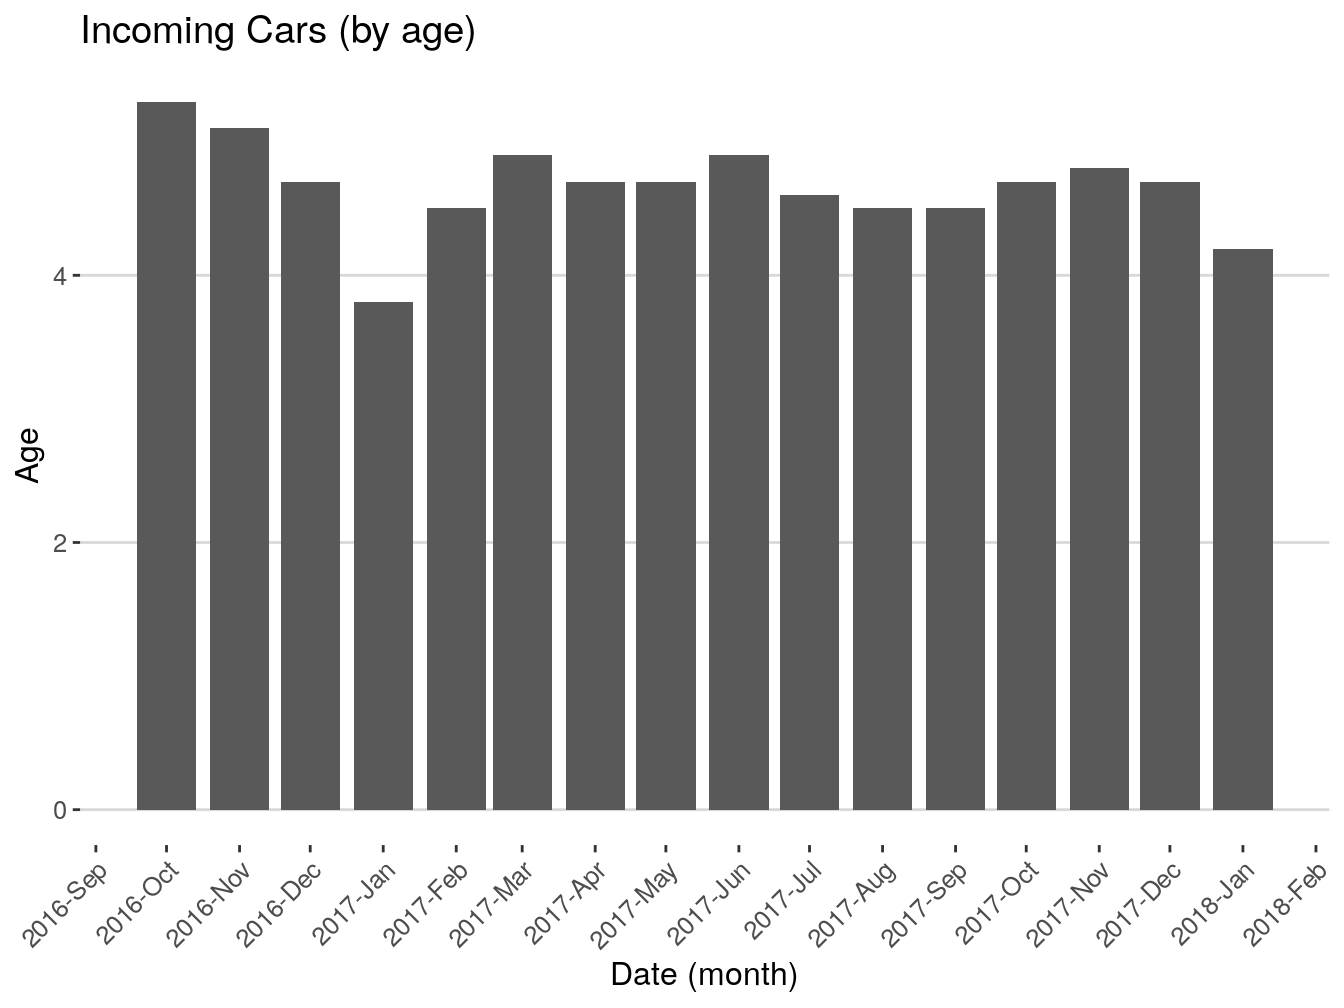
\includegraphics[width=1\linewidth]{bookdown-demo_files/figure-latex/nice-fig65-1} \end{center}

Great! This concludes our introduction to the basics of ggplot2(). When you done and comfortable with your plots, it is time to export them. The simpliest way to do this is to got to the plots tab in the lower left corner of Rstudio, selext Export and save it as an image, for example (see Image export demo pic). The next step is to open a Word Document, write a narrative and paste the images in there. I hope I do not need to show you how to do that. If I do, you are really in the wrong place.

\begin{figure}
\centering
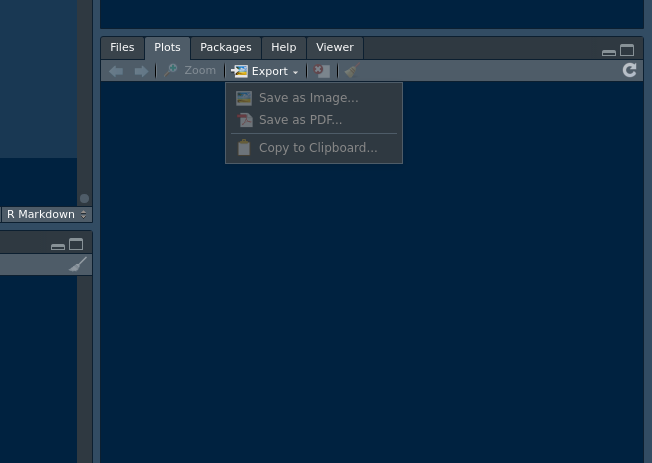
\includegraphics{imageExport.png}
\caption{Image export demo.}
\end{figure}

\hypertarget{r-markdown}{%
\subsection{R Markdown}\label{r-markdown}}

Although, Word is not a bad solution for reporting our findings, R has a much more convenient tool that takes a regular Word report and injects it with steroids. Again, I am not going to go deep on this topic because it is too big. I will show you the basics to get you started. The first thing you need to do is installing r markdown. Run install.packages(``rmarkdown''). You do not need to write `library(rmarkdown) in this case, Rstudio knows. Before we start, install another package - 'stringi'. This package provides some tools for working with text, but we will need it to generate random text for our markdown report.

Before we proceed, lets save the final tables that we used to generate our plots. We could copy and paste the code that we used to get to these tables, but why do that if we already got what we need.

\begin{Shaded}
\begin{Highlighting}[]
\CommentTok{# Saving.}
\KeywordTok{fwrite}\NormalTok{(dataForLine, }\StringTok{'dataForLine.csv'}\NormalTok{)}
\KeywordTok{fwrite}\NormalTok{(dataForFuelLine, }\StringTok{'dataForFuelLine.csv'}\NormalTok{)}
\KeywordTok{fwrite}\NormalTok{(dataForBarPlot, }\StringTok{'dataForBarPlot.csv'}\NormalTok{)}
\end{Highlighting}
\end{Shaded}

First, create a folder inside of the folder with the current project. Name it `markdown' or something. Now, open a completely new Rstudio session. Your screen should look like the illustration below. Click on `File' -\textgreater{} `New File' -\textgreater{} `R Markdown\ldots{}'.

\begin{figure}
\centering
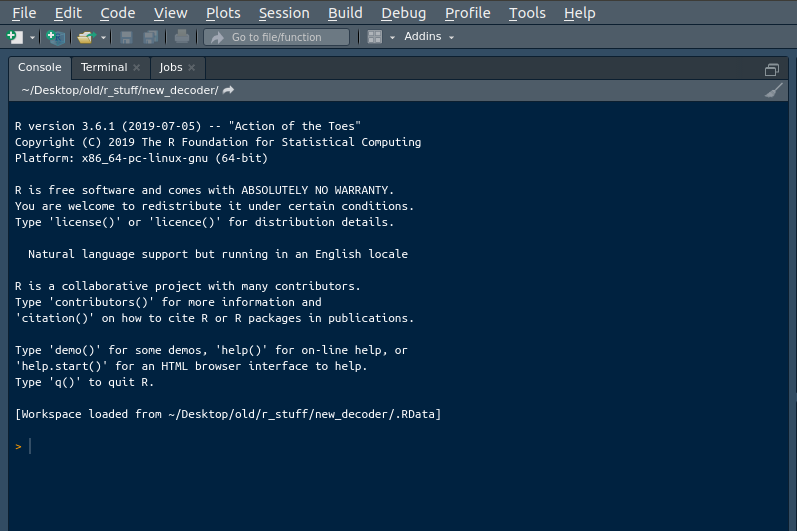
\includegraphics{newSession.png}
\caption{New session.}
\end{figure}

You will see a new markdown file window like below. A markdown project can result in different final formats, but we are only exporing HTML now. Name your markdown something and specify the author. Click `OK'.

\begin{figure}
\centering
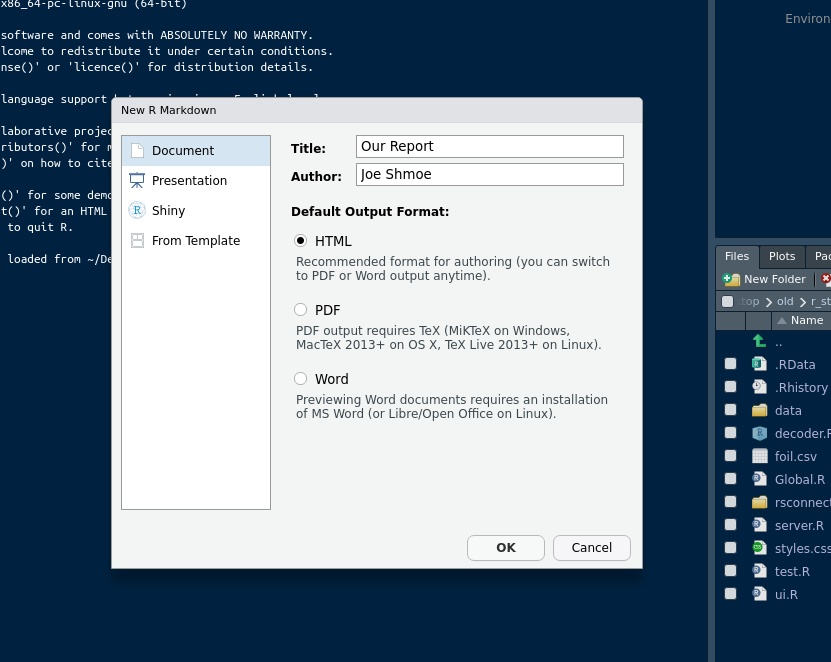
\includegraphics{newMarkdown.png}
\caption{New session.}
\end{figure}

Another great thing about Rsudio is that it provides templates for many different things. When we will be discussing APIs, Web Apps, and other things, you will see how useful it is to have a code tepmlate to get you started. Markdown is not different. Below, Rstudio gives you a working template of how a markdown document should look like. Lets go through the template to see what it consists of. There are five parts that I can identify. The first is a `hat'. This is where the information and parameters of the markdown go. It is surrounded by the tripple dashes. The second is the general space where you can specify titles, write text, and in-line code. The third is a `chunk'. Chunks are bulding block of a markdown document. Any code that we wrote and ran so far in this book, we can run inside a chunk. To created a chunk, you need to write two sets of tripple ticks. The space between them will be your chunk. The fourth element comes after the first set of tripple ticks and is surrounded by curly braces. This is where you specify chunks parameters. There are many different parameters that you can specify there. You will see all that for yourself when you will start experimenting with markdowns, however, I will just give you a few most freqient parameters and what they do. When you press `knit', the code that you write in those chunks gets executed line by line just like in regular R file. In most cases, you will not want the reader of your report to see the code behind your findings. The parameter `echo = False' takes care of that. Also, as you might have noticed, any code can produce a bunch of warnings or messages. There are parameters for that too. There are parameters for width and height of your charts or illustrations, and a bunch of other crap as well. If I start to list all of them here, you will not remember. It is better if you just google them on case by case base when you need them. The fifth part is the actual code that you include in a chunk. As I mentioned before, the code in the chunks runs just the same as the one that you have been practicing with so far. The difference here is that it is sectioned by chunks and you can apply different rules (parameters) to each chunk. These are the main five parts of a markdown. There are, obviously, more sub-parts, but you do not need to worry about them right now.

\begin{figure}
\centering
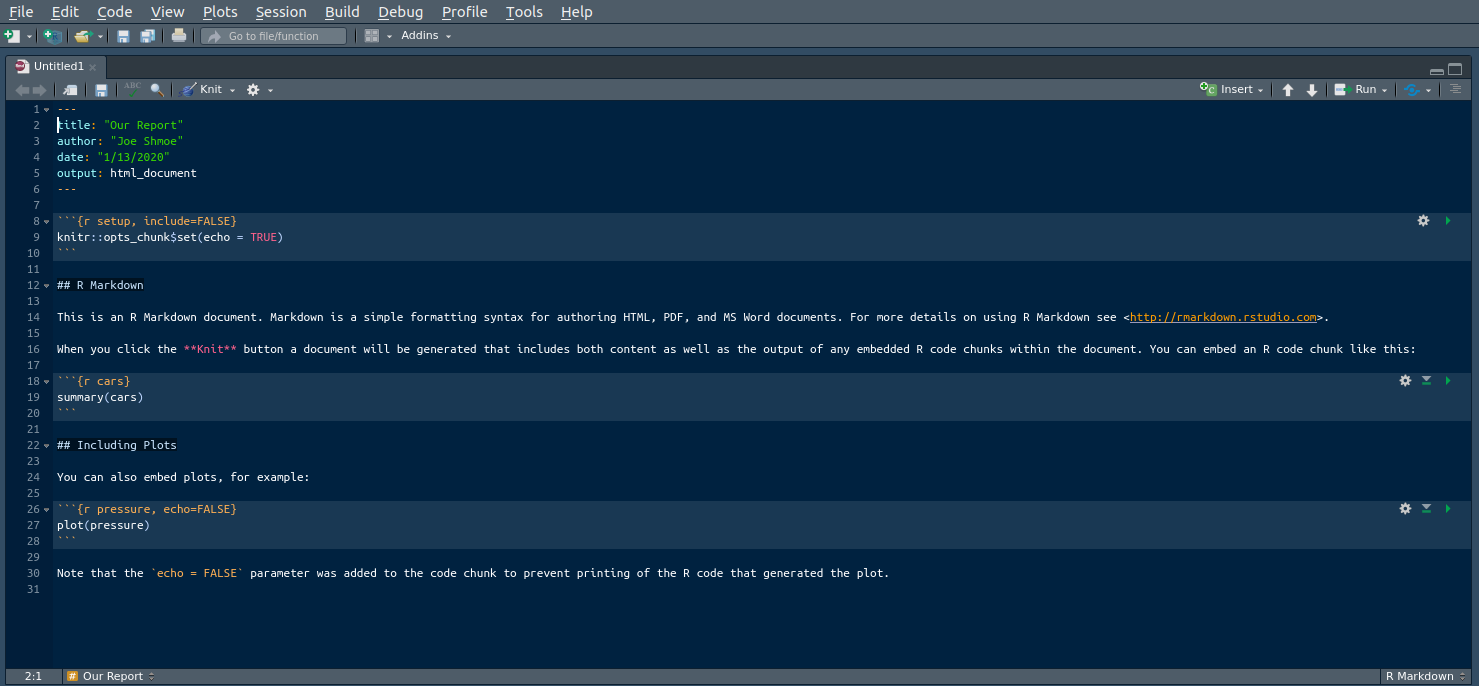
\includegraphics{markdown1.png}
\caption{New session.}
\end{figure}

Although, it is just a template, since we have already specified the title and author we can see them in the `hat' of the markdown. The hat of the markdown is where you specify different parameters for the final document. The parameters can be font, spacing, color, themes, and more. Although, it is just four lines now, it can get much much bigger. Everything else is generic now. Click the `Knit' button above the `hat' to see what the final document will look like.

\begin{figure}
\centering
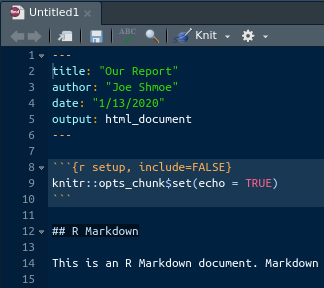
\includegraphics{markdown2.png}
\caption{New session.}
\end{figure}

Pretty cool, right? R and Rstudio makes it extremely easy to go from doing research and writing code to presenting it in a widely accessible format. If you have not noticed yet, the document that you just produced is an html. This means that any browser can open your report. It might not seem like a big thing, but presenting your stuff from outside of your own computer can be a really big fucking problem. Many tools that are popular now are very close-ended and will not let you do shit from ouside, unless you give them your kidney. Anyway, your template report should look like mine. Go through it, compare side by side with the template's code, see what corresponds to what.

\begin{figure}
\centering
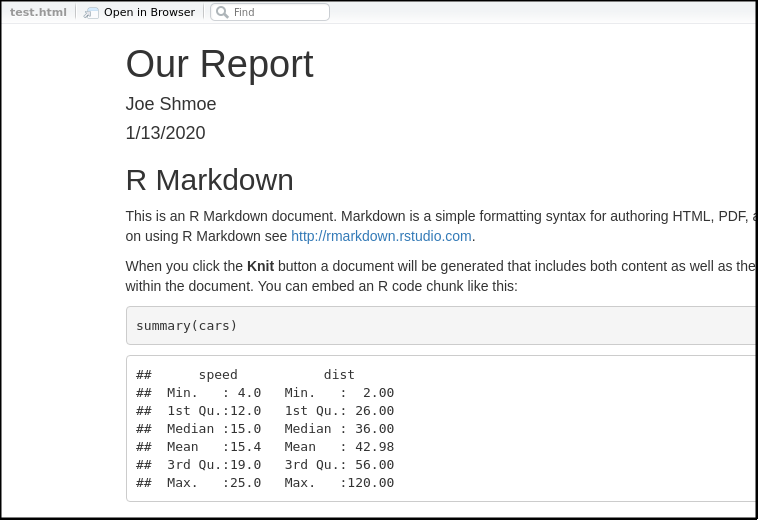
\includegraphics{markdown3.png}
\caption{New session.}
\end{figure}

Lets use our plots to create a markdown report. First, eliminate everyhing except the `hat'. The first chunk will only hold the libraries that we will be using for the code to generate the report. Just copy the ones that we used so far. Use the illustration below for reference. If not sure, just copy and paste all the libraries that we have been using so far. One thing about markdowns is that it will not render if something is missing or broken, and it will not tell you why in most cases. So, even if one library is missing, it will not render. It is actually batter to include more libraries than you need than less because of that. Then , create a chunk with two sets of tripple ticks. Inside of the curly braces you want to specify three things: 1. Engine (r) - mandatory, 2. Chunk name (libraries) - optional and must be different for each chunk, 3. Include = False - optional. The `include = false' parameter will run the code but will not print or display it in any way, so our libraries will be loaded but we will not see all those garbage messages that come with them. Press `knit' and you will see an empty report with the hat information.

\begin{figure}
\centering
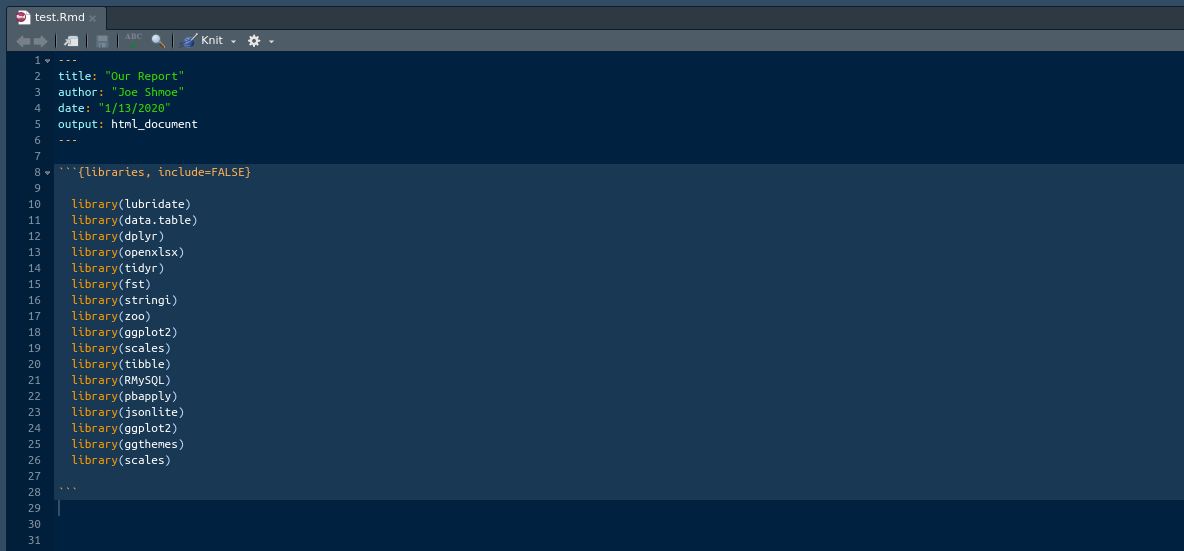
\includegraphics{markdown4.png}
\caption{New session.}
\end{figure}

Ok, lets start simulating a real report. You can write any text outside of your chunks. On top of that, you can specifiy headers and write in-line code there. There are three types of header in markdown. The main header has to prefixed with the single `hash' (\#) sign. The middle one has two hashes. The smallest has three. In order to write in-line code, you have to surround it with a set of single ticks. Inside goes the engine (r) and the code. Check out the illustration below to see the examples of both. The function stri\_rand\_lipsum() generates a paragraph of random text for us. Knit it to see what it looks like.

\begin{figure}
\centering
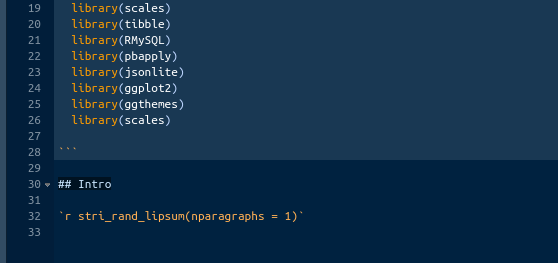
\includegraphics{markdown5.png}
\caption{New session.}
\end{figure}

At this point, we have covered the core of the shit that we need to know about markdowns. From now on, we will be just copying an pasting our plots code and filling the voids with some generic text. Lets create a new paragraph with a middle-size header called `Line Plot' and random text. After that, create a chunk with the following parameters: \{r, echo = False, error = False, message = False, message = False, fig.aling = `center\}.
Lets go over the parameters. The first one is the engine, in other words, the language that we are using, which is 'r'. The next one is `echo = False'. Echo works just like the `include' that we used in the first chunk. The difference is that `echo' will render the result of the code but not the code itself, and `include' will not display anything if set to `false'. The next three parameters are `error', `message', and `warning'. These three are very similar as they block or display errors, messages, and warnings. We do not need any, so we are setting them to `false'. The final parameter is `fig.align'. We want our plots at the center of the screen, so we are setting it to `center'. Again, you can include more parameters here, but we do not need to now. Now, we are ready to render our first plot. As you should remember, we saved the result of our aggregations for the line plot as `dataForLine.csv'. Lets read it back to this chunk. Type dataForLine \textless{}- fread(`dataForLine.csv'). We need to convert the date to the date format as it flipped to the character type in transitions. I hope, you remember how to do that. If not, go back. If can not, reference the illustration below. Finally, just copy and paste the code we used to generate and output the line plot (see the illustration below for reference).

\begin{figure}
\centering
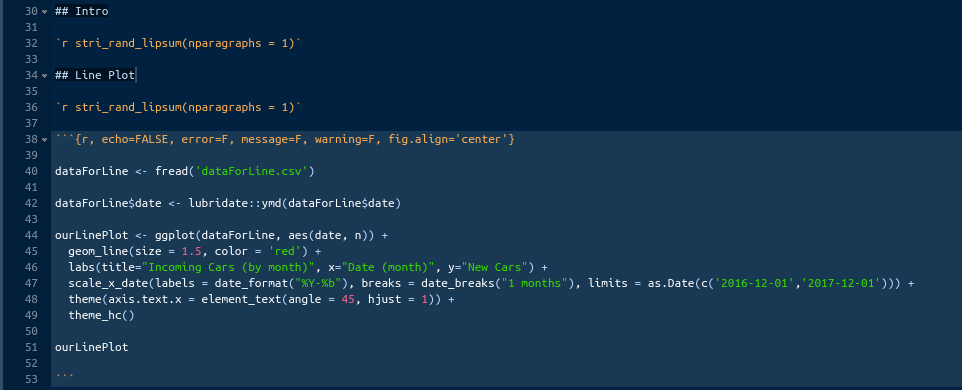
\includegraphics{markdown6.png}
\caption{New session.}
\end{figure}

Knit the file and your report should look like the illustration below:

\begin{figure}
\centering
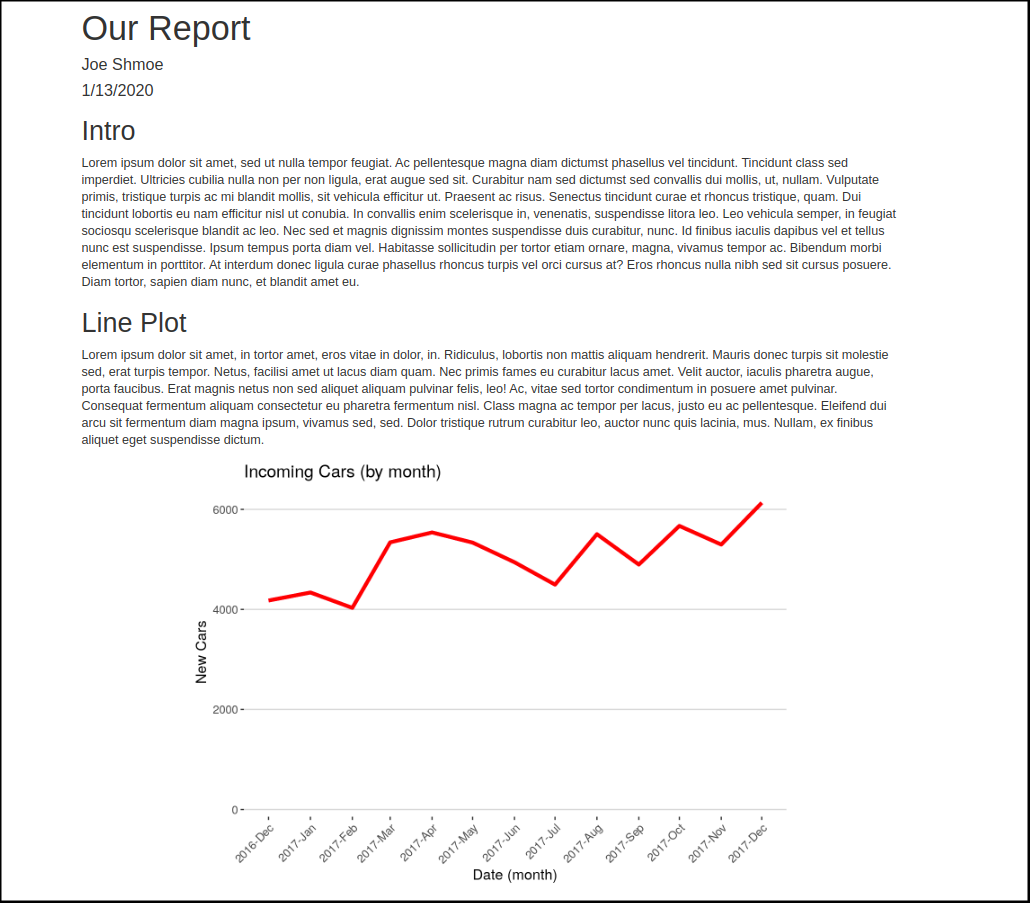
\includegraphics{markdown7.png}
\caption{New session.}
\end{figure}

So far, we got the hat, introduction, and the first plot. The rest of the report will be the same. After the second chunk create another mid-size header `Line Plot (by fuel)'. Add another random text paragraph under it and create another chunk with the same parameters as in the previous one. Load the `dataForFuelLine.csv' to this chunk, fix the date column, and copy and paste the second plot code in here. Reference the illustration below if stuck.

\begin{figure}
\centering
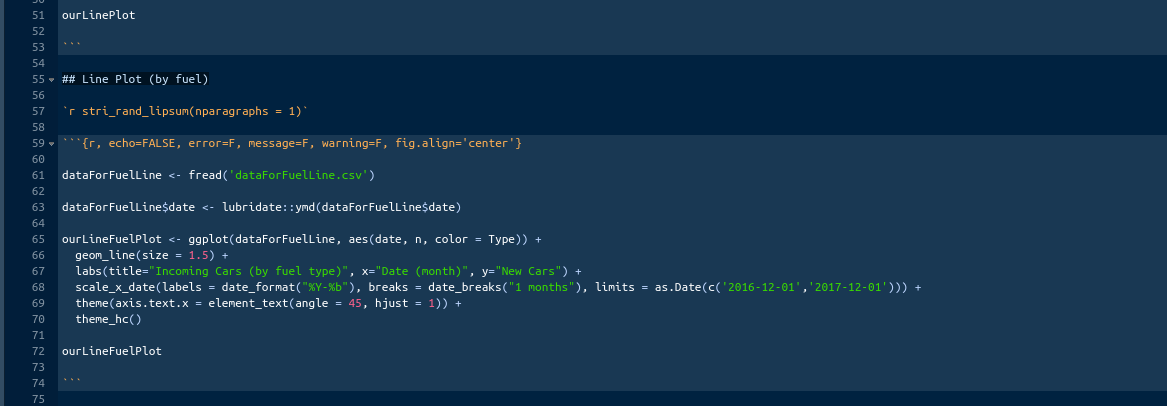
\includegraphics{markdown8.png}
\caption{New session.}
\end{figure}

Repeat the same steps for the bar plot this time. You can name things as you see fit. refer to the illustration below if confused. After the final chunk, create another mid-size header `Conclusion' and add another paragraph wiht generic text to complete the report.

\begin{figure}
\centering
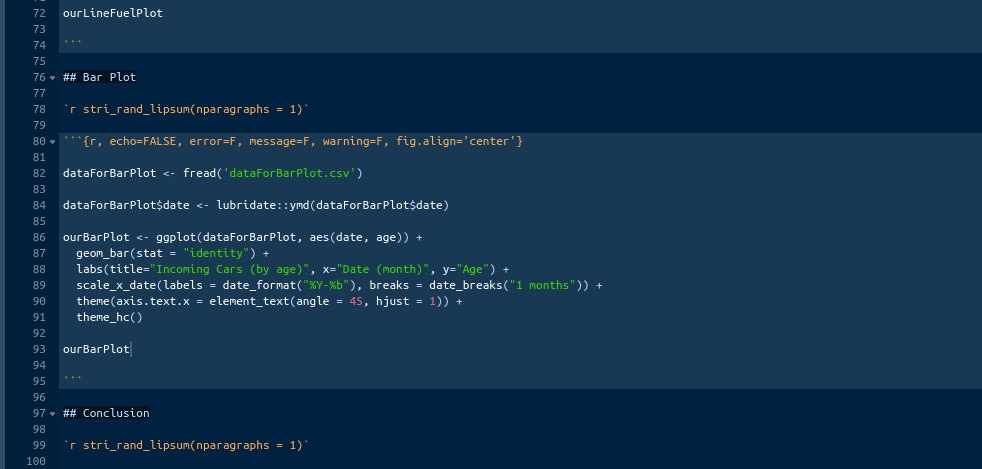
\includegraphics{markdown9.png}
\caption{New session.}
\end{figure}

Finally, I want to show you how to add a table of contents (toc) to our report. The toc will be linked to the headers that we created. A markdown's `hat' is very particular about formatting. If you want things to work as intended, you must make sure that punctuation and indentations are correct. To add the toc, change the hat exactly like I have it in the illustration below.

\begin{figure}
\centering
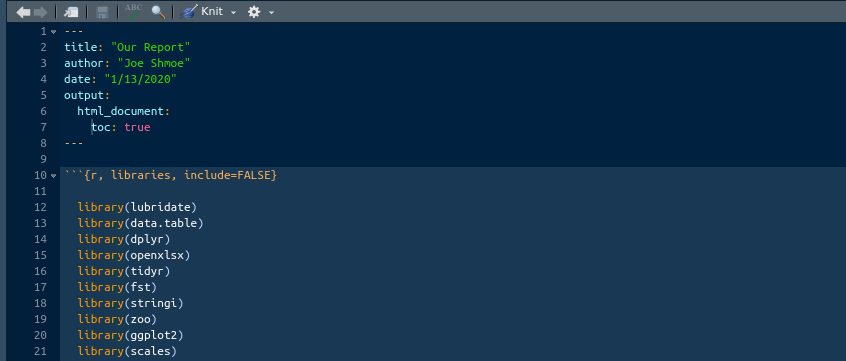
\includegraphics{markdown10.png}
\caption{New session.}
\end{figure}

Knit the report and the toc will look like the illustration below. You can now click on any entry and you will be navigated to it. Give it a go.

\begin{figure}
\centering
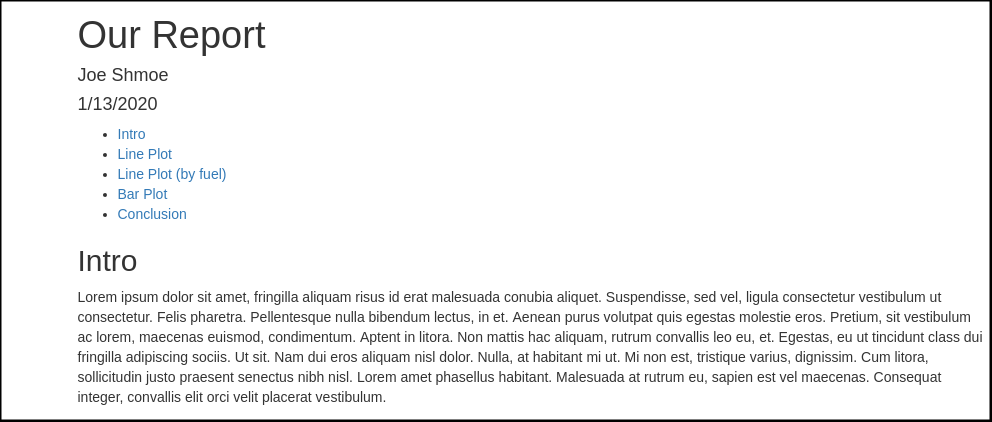
\includegraphics{markdown11.png}
\caption{New session.}
\end{figure}

We are done with our report. You final document should look like this. Pretty fucking awesome.

\begin{figure}
\centering
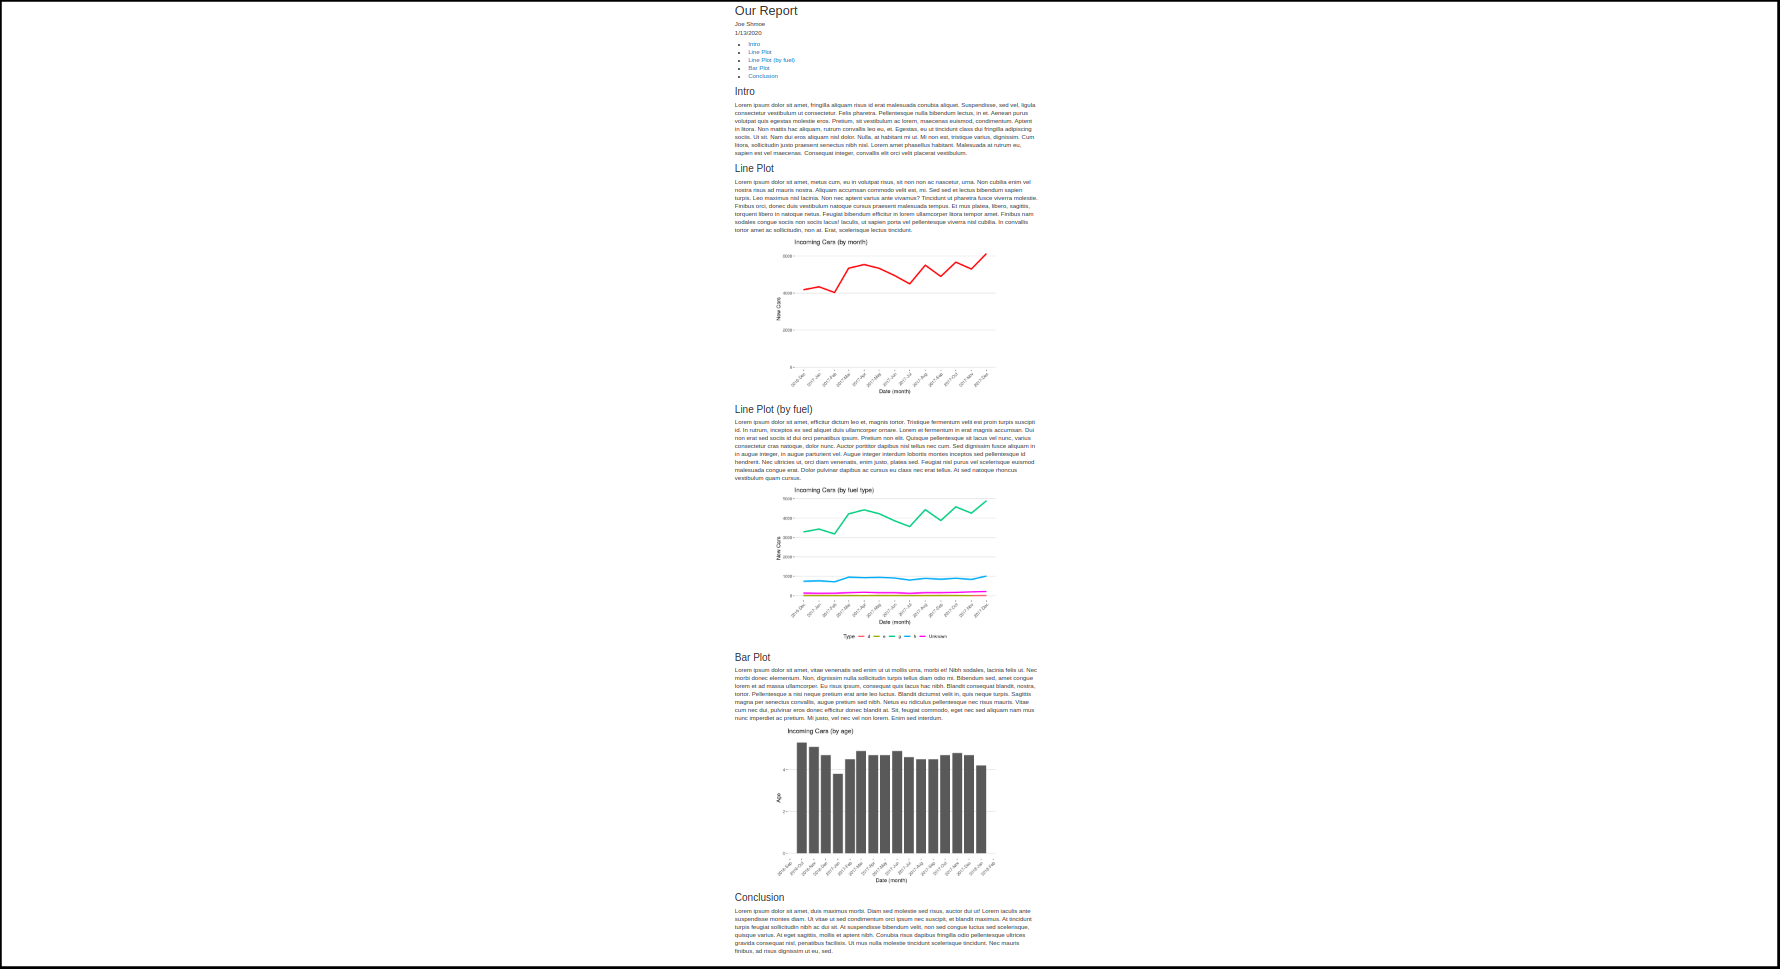
\includegraphics{markdown12.png}
\caption{New session.}
\end{figure}

Now you have some basic understanding of Rmarkdown. You know how to generate it and how to properly structure your reports. On top of that, this section leaves you with not a bad template for some basic reporting. Obviously, there are many more things that you can do with a markdown, but we are not covering that in the introduction to everything in R. However, what you know now should be a good foundation to start exploring other capabilities of Rmarkdown. Personally, I never had the need to do with markdown more than I just showed you. So, whatever we have covered will be already enough more the most of you. Having said that, Rmarkdown is important to at least be familiar with.

\hypertarget{bonus-1}{%
\section{Bonus}\label{bonus-1}}

Remember I said that I will show you how to make your plots more informative. Now is the time. The trick that I am about to show you was a gateway for me into the topic of interactive visualization. It would be cool if we could just take the ggplot that we created and start interacting with it. We would not need to dance around looking for adhoc solutions to improve the informativeness. Meet the package `plotly'. Plotly is a JavaScript library that is heavily adopted and used in R to create interactive visualizations. First thing you need to do is install the package. Type install.packages(`plotly'). Once it is done installing, I want you to change the first chunk of your markdown to the following illustration:

\begin{figure}
\centering
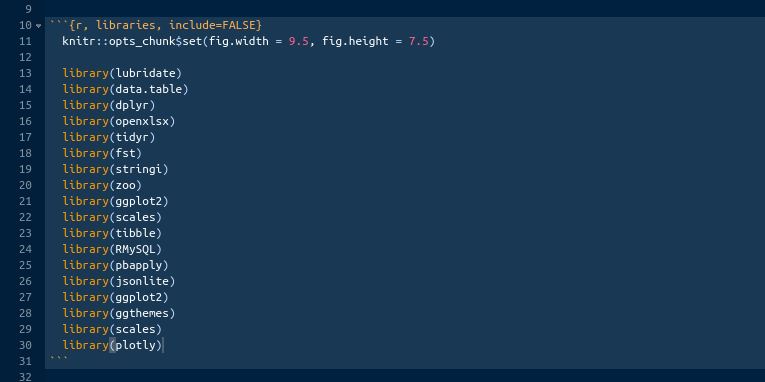
\includegraphics{markdown13.png}
\caption{New session.}
\end{figure}

There are two additions: 1. knitr::opts\_chunk\$set() specifies the global parameters for all chunks. In this case, the plot dimensions. 2. library(plotly) - I should not explain this one. Now, to the trick itself. Plotly is just like ggplot2. We can use plotly to create any interactive chart from scratch just like we did in ggplot2. That is the whole topic and we will not be doing that. The reason I am refering to this part as a `trick' is because we can just take out plots that we created in ggplot2 and wrap them with the plotly function ggplotly(). That function will take all the parameters, bells, and whissles, and will generate a plotly plot with them. Lets do it. Take every chunk that generates a plot and wrap the final variable with the ggplotly() function like so: ggplotly(ourLinePlot). Do it for all three of them.

\begin{figure}
\centering
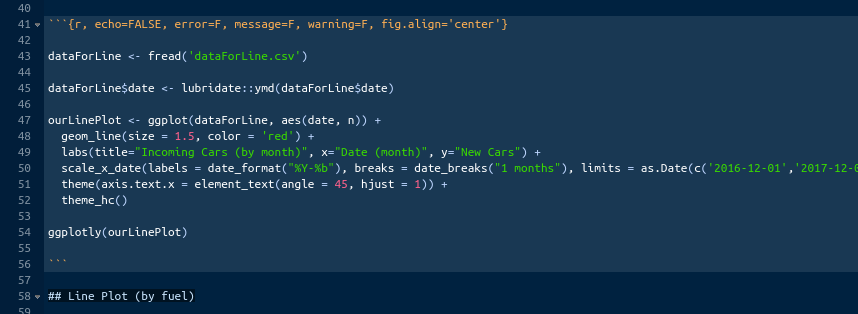
\includegraphics{markdown14.png}
\caption{New session.}
\end{figure}

Knit the report again and you should end up with the report that is very interactive. You can zoom in, take a snapshot, hover to see the numbers, select and deselect data, etc. It is really fucking awesome for basically no effort. Most importanly, it makes your report stand out.

\hypertarget{you-are-not-a-r-maggot-anymore}{%
\section{You are not a R maggot anymore}\label{you-are-not-a-r-maggot-anymore}}

Congradulations, you are not a R maggot anymore. This is the end of your big assignment. You went far beyond what was expected of you. You will present this report to your supperiours and they will be very impressed with your progress while you are in front of them. They will definitely forget about you the next minute but that is not the most important part. The most important is that you have proven to them and to yourself that you can take something really complex and completely new to you and master it in a short period of time with minimum or no supervision. Let me remind you what you were tasked to do. You were given the code that your superviser has been working on for months. That code already worked and you just needed to tweak it a bit more. I got to tell you that the majority of people would just run the code, encounter an issue or two, and run for help as soon as things got tough. Forget about improving the code and building things on top of it. Best case scenario, they would just run it from time to time and periodically lean on you to do what, really, is expected of them. You will encounter that kind of attitude a lot and it is important that you yourself do not fall into the trap of relying on others for something that you must do. That is particular important in programming. Nobody is going to do the learning for you. If there is one thing that I wanted you to take from this book, that would be the steps and attitude we took to solve our big assignment. Applying the strategy that I showed you for the next year, combined with hunger, will make you an expert in R and will take you to the level where you will be able to teach others, just like I am teaching you now. With this settled, lets see what we have actually done in this section and what it means for us.

First, we were given a very complex, for us back then and for most now, code and tasked with understanding it and running it periodically. We were given two to three months for that. We had no idea what the code was doing and what any of it meant. We ran it line by line to see what each piece of it did. We learned how to connect to a database, pull data that we need from it, aggregate that data using various R function, and save the result. In the programming world, this is called `ETL' (Extract, Transform, Load). Although, we went over the code many many times and understood the outcomes of each line, some parts of it were still very hard or impossible to understand without deeper understanding of R. Here, I mean the NHTSA API call.

Along the way, we learned about a thing called `Tutorial Purgatory' and how to avoid getting sucked into it. We dove deeper into working with dates and times and learned the one library that we will be sticking with for a while (lubridate)

Second, we decided to see if we could rewrite the same code in a more staighforward way. The biggest improvement that we were able to make was to the API call. I, still, do not expect you to fully understand that thing, but at least it became much easier to, compared to the monstrosity that it was before. After we rewrote the code, we should have gotten a better grasp of it. At that point we were doing things that we will be doing ninty percent of a time from now on, give or take a few things. We presented our progress and were ready to start building on top of it. We impressed our supervisor and were given our addon assignment.

Third, we got tasked with adding `Miles per Gallon' (mpg) information for each vehicle from now on. There was no clear procedure for that. We had to be creative and more importantly knowledgeable in R to get something like that done. The fact that we got an assignment like that showed that we demonstrated our capacity to independently do something like that. The problem with that task was the lack of unique identifier that we could use to join the fuel dataset with our vehicles dataset. That particular problem taught us how to write ugly but working code. We are no longer intimidated by the majority of tasks because we know that they will probably not be much harder than this one. And if they are, we will be able to dissect, understand, and complete them. The most important thing that we took from that part was confidence.

Finally, we dicided that it would be proper to present our efforts in a nicely formatted report. We learned a lot about ggplot2 library and generated a few plots. From experience, in ninety percent cases, you will not need more ggplot2 than we have covered here. After covering plots, we leaped forward and covered a lot of ground on Rmarkdown. That will be extremely useful for you if your job requires a bunch of reports. Markdown is the standard for that kind of stuff and, again, we covered just enough so you can tackle the most of the tasks thrown at you. Obviously, you might requre different parameters for your chunks, but you got the template and knowledge that you can work with already. Finally, as a bonus, we converted our static ggplot2 plots into dynamic plotly plots, which made our report more impressive and informative. More importantly, it took our skills to the next level and opened the doors to the topic of dynamic visializations.

The big assignment is over, the topics that will follow are important but are not core. Pat yourself on the back, you are not useless anymore!

\hypertarget{maps}{%
\chapter{Maps}\label{maps}}

At the end of the last chapter, we opened the doors to the topic of dynamic visialization with converting our static ggplot2 plots to dynamic plotly plots. We will continue moving in that direction from now on. One thing that fucking facinated me at the beginning was mapping. I did not understand how it was done and it seemed extremely complicated. I honestly thought that you had to write code to display every single element of a map. Well, you do need to write code to display things, but it is way easier than I thought. I would walk around the office drooling over the people who could do mapping thinking that it was out of reach for me at the moment. Until I reached that topic and saw that it is nothing compared to what I already knew. Maps are extremely important though. If you decide to continue with the rest of the series, you will see that we will be building a huge chunk of our progress around mapping. Obviously, there are things in maps that are very complex. For those things, you will have to get a dedicated book or a course. But, as usual, whatever we will cover here will be more than enough for your day to day work and will definitelly take you to the next level.

\hypertarget{maps-different-libraries}{%
\section{Maps, different libraries}\label{maps-different-libraries}}

There are a few libraries that can draw you a map. I will mention three of them and will show you how to use only one. Only one, but the best one and the only one that you will need. I will explain why here. Just like with plots, maps can be static (just a picture) and dynamic (interactive). They can even be 3D, but we do not need that. You have already see the limitations of the static plots. My question is then: why the fuck do we even need static maps? Someone who knew what they were talking about could say: they are easier to save and overall lighter than dynamic maps. The first one is bullshit, because if you want a png of the dynamic map, you can just focus on the area of interest and take a snapshot. That inconvenience is nothing for the flexibility that a dynamic map can provide. The argument about the size difference is valid. If you have a heavy (cpu or ram demanding) web application or script, then downgrading to a static map is one of the options for optimizing performance. However, as I mentioned before, first we will learn to get things done no matter what. If you at the point where you need to start optimizing things, then congradulations, you do not need my books anymore. Trust me, at that point, you will be able to use both static and dynamic maps. Here, I will show you the most useful and exciting way to work with maps. If you get interested in the topic, please, go ahead and start lookin deeper into it elsewhere.

\hypertarget{ggplot2}{%
\subsection{ggplot2}\label{ggplot2}}

The library ggplot2 can also draw static maps. For the reasons outlined above, I will not go deep into generating maps using ggplot2. However, I do want to show you an example of how easy it is to create a map and what a static map looks like. Lets draw an empty map of the US. Before we begin, open a new R file and type install.packages(`maps'). We will not need to load it though.

First, we need to get the data that ggplot2 will you to paint the map. The ggplot2 library comes with the function map\_data(). This function turns on outline of a shapefile into a dataframe where latitudes and longitudes of each point become columns. We can then use that dataframe to plot those points using standard ggplot2 sintax from before.

Getting the data to create the map of USA. Open it to see what those columns that I just talked about look like.

\begin{Shaded}
\begin{Highlighting}[]
\CommentTok{# Getting the map.}
\NormalTok{  usa <-}\StringTok{ }\KeywordTok{map_data}\NormalTok{(}\StringTok{"usa"}\NormalTok{)}
\end{Highlighting}
\end{Shaded}

Standard ggplot2() sintax:

\begin{Shaded}
\begin{Highlighting}[]
\CommentTok{# Map.}
\NormalTok{  ourMap <-}\StringTok{ }\KeywordTok{ggplot}\NormalTok{(}\DataTypeTok{data =}\NormalTok{ usa, }\KeywordTok{aes}\NormalTok{(}\DataTypeTok{x=}\NormalTok{long, }\DataTypeTok{y =}\NormalTok{ lat, }\DataTypeTok{group =}\NormalTok{ group)) }\OperatorTok{+}\StringTok{ }
\StringTok{  }\KeywordTok{geom_polygon}\NormalTok{()}
\CommentTok{# Calling the map  }
\NormalTok{  ourMap}
\end{Highlighting}
\end{Shaded}

\begin{center}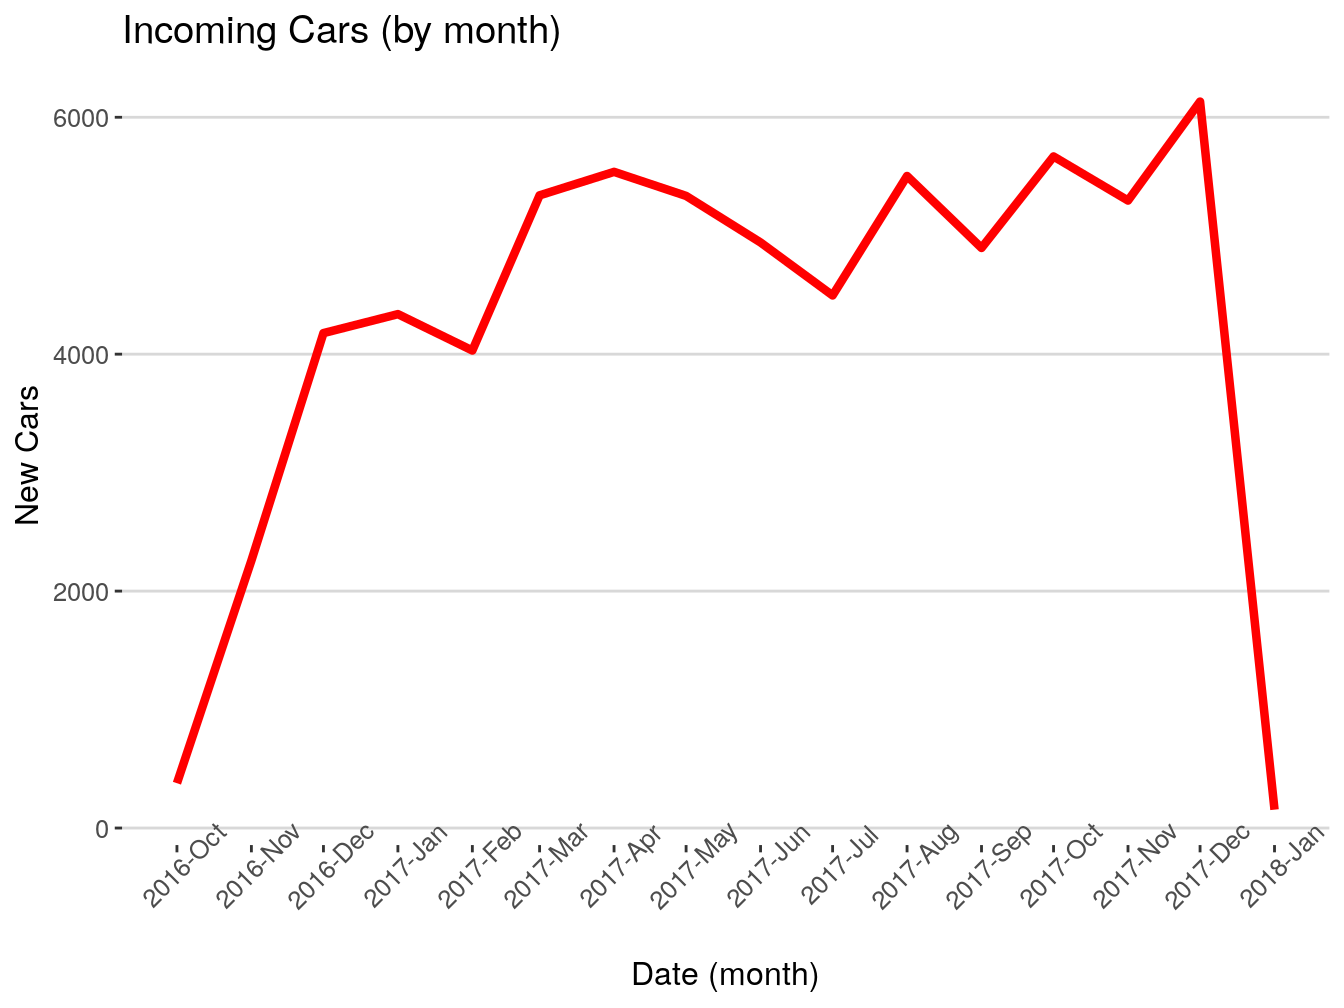
\includegraphics[width=0.9\linewidth]{bookdown-demo_files/figure-latex/unnamed-chunk-229-1} \end{center}

Just like with the line and bar plots that we generated in the previous chapter, we are using the ggplot() function, the `+' sign and then specifying the `geom\_\ldots{}' command. The difference here is that we used the geom\_polygon() to draw a map instead of the geom\_line() or geom\_bar() to draw plots.

As you can see it is not too complicated. In total, we wrote five lines of code and got a map. There is not doubt, if you master the ggplot2 you can draw some amazing plots and maps with it. Mastering ggplot2 is not our goal here, which is why we are going to move on.

\hypertarget{ggmap}{%
\subsection{ggmap}\label{ggmap}}

The ggmap library is very similar to the ggplot2. The syntax is very similar and the whole process of gradually layering things on top of each other is the same. The output is static as well. The difference is that ggmap allows you to work with basemaps (background). A basemap is like an atlas. When we generated the shape of the United States, there was nothing behind the shape, just a blank canvas. If we did the same using ggmap, we would see the water, states, and many other things depending on the basemap we selected. It is better if I demonstrate. Before we proceed, type: install.packages(ggmap).

It is pretty much the same as with the ggplot(), even easier. Instead of five lines, we will do it in four.

\begin{Shaded}
\begin{Highlighting}[]
\CommentTok{# Getting the basemap}
\NormalTok{ourBasemap <-}\StringTok{ }\KeywordTok{get_stamenmap}\NormalTok{() }

\CommentTok{# storing the map inside of a variable}
\NormalTok{ourGgmap <-}\StringTok{ }\KeywordTok{ggmap}\NormalTok{(ourBasemap) }

\CommentTok{# rendering the map}
\NormalTok{ourGgmap}
\end{Highlighting}
\end{Shaded}

\begin{figure}

{\centering 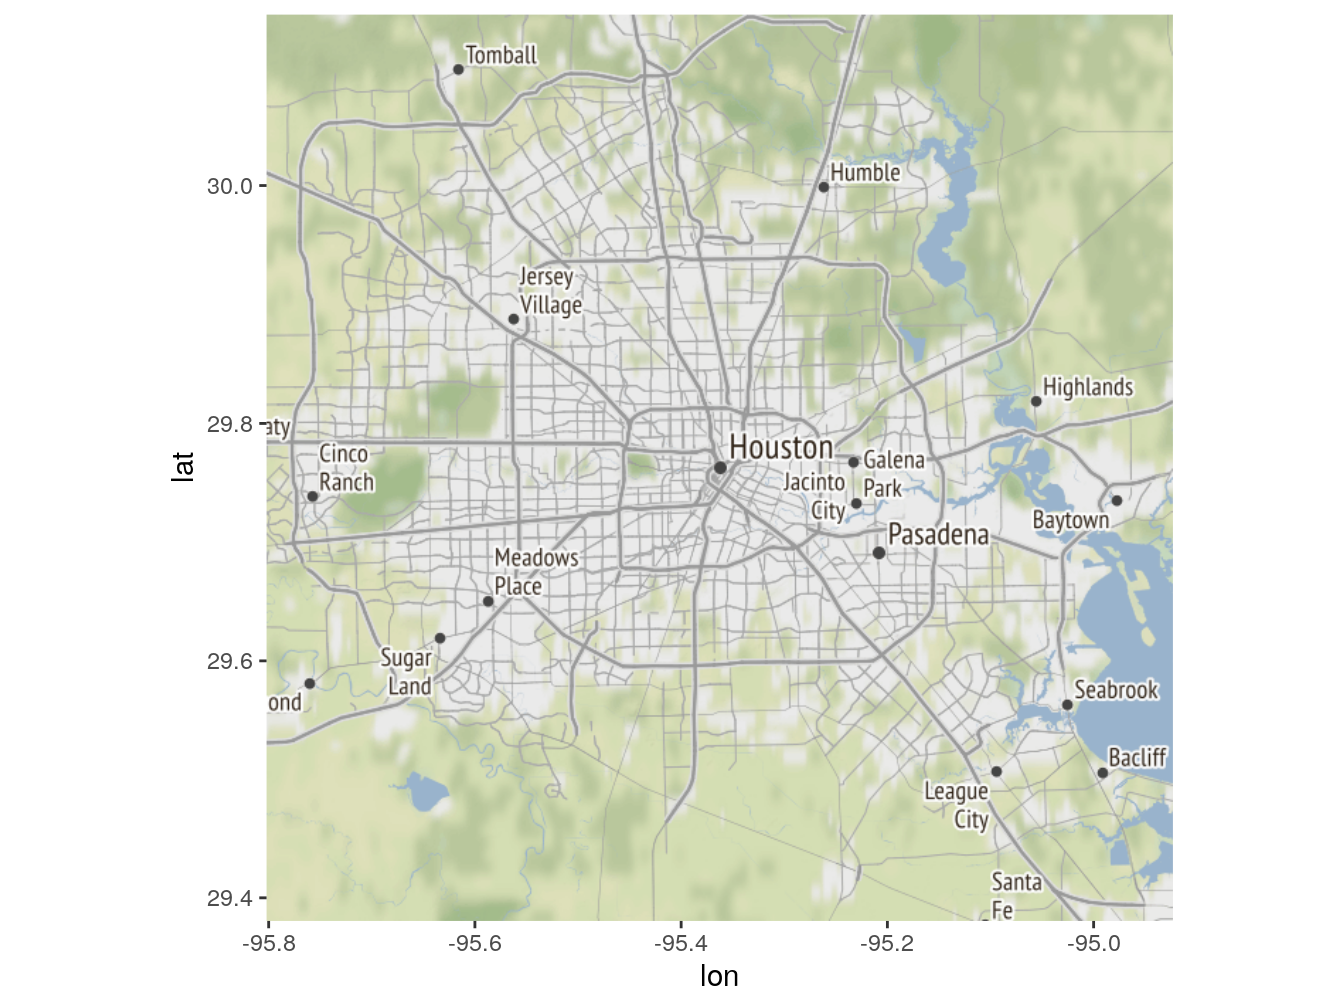
\includegraphics[width=0.9\linewidth]{bookdown-demo_files/figure-latex/nice-fig70-1} 

}

\caption{Here is a nice figure!}\label{fig:nice-fig70}
\end{figure}

Nice. Not really though. It is the same shitty static map. It can be useful here and there, but for the reasons that I talked about in the beginning of this section, we will not be using ggmap either. Nevertheless, now you are familiar with both main libraries for generating static maps. I, actually, wanted to skip ggmap library demonstration altogether, because Google now requres us to create an account with them in order to use their basemaps. That is a big annoyance, especially when you are just learning and do not really know how to use `api keys' and other shit that they want you to do. When you are learning, you just want shit to work. Adding that extra layer of complexity is just not worth it, considering that, in my opinion, ggmap is not even that great. Lets move on to what we came here for.

\hypertarget{leaflet}{%
\subsection{Leaflet}\label{leaflet}}

Taken from the leaflet's docummentation page on GitHub: ``Leaflet is one of the most popular open-source JavaScript libraries for interactive maps. It's used by websites ranging from The New York Times and The Washington Post to GitHub and Flickr, as well as GIS specialists like OpenStreetMap, Mapbox, and CartoDB.'' Leaflet is extremely popular. It is a JavaScript library, but it is adopted by R so well that it is actually much easier to use it in R than in JavaScript. I did both. I do not want you to think that I am bullshitting you right now, so let me shock you with how awesome and simple it is righ away. Type: install.packages(leaflet). After it is installed, lets load the library and render our first leaflet.

\begin{Shaded}
\begin{Highlighting}[]
\CommentTok{# Loading the library.}
  \KeywordTok{library}\NormalTok{(leaflet)}
\end{Highlighting}
\end{Shaded}

Just one line this time.

\begin{Shaded}
\begin{Highlighting}[]
\CommentTok{# rendering the map}
\KeywordTok{leaflet}\NormalTok{() }\OperatorTok\StringTok{ }\KeywordTok{addTiles}\NormalTok{()}
\end{Highlighting}
\end{Shaded}

\hypertarget{htmlwidget-62f2cfa9836887bc9ab5}{}

\label{fig:nice-fig72}Here is a nice figure!

How cool is this? With just two lines of code you got a fully dynamic map that you can iteract with. Go ahead and be amazed of how much better it is compared to that static crap, and how much easier it was to render it. The first time I saw it, I knew that, unless there is a major compromise associated with using it, I will not be going back to static maps. Now that you stoped drooling over that map, lets talk about leaflet a bit more. After that, I will show you a lot of cool stuff that you can do with it. As always, not too much, but just enough to get you started.

\hypertarget{leaflet-deeper-dive}{%
\section{Leaflet, deeper dive}\label{leaflet-deeper-dive}}

I know that I praised leaflet a lot already, but I am not done yet. Leaflet, along with plotly and shiny (which we will cover later) gave a huge boost in terms of my drive to learn R and code in general. Going through dry tutorials and hundreds and hundreds dry lines of code gets very boring at some point. Some people do enjoy coding just for the coding part, others enjoy crunching numbers and solving problems, however, the majority of us want to be entertained from time to time. Crunching numbers and solving problems can be entertaining too, but when you are just starting, in most cases, you need that tangible progress. Not many things in programming are more tangible than making things move on the screen. That is why giving yourself a boost by learning how to inject interactivity in your code will get your further than just sitting and learning dry code. It definitely worked for me.

Before we move to our routine of pulling data from a database, messing with it, and outputting it on a fancy map, I want to go through some leaflet basics. Basically, I want to show you how to place a dot on a map and play with a few parameters. You do not actually have to follow my tutorial on this if you hate me already. Leaflet has an amazing and simple tutorial on their GitHub page, just google `leaflet R'. But if you still tolerate me, keep reading.

Lets see what each part does and what kind of things we can layer on top. First, we will call the leaflet() function without anything else to see if it does anything.

\begin{Shaded}
\begin{Highlighting}[]
\KeywordTok{leaflet}\NormalTok{() }
\end{Highlighting}
\end{Shaded}

\hypertarget{htmlwidget-b210fa06e4fef6405837}{}

\label{fig:nice-fig73}Here is a nice figure!

Apparently, it provides an empty canvas with some basic functionality. The difference between this and the one before is the addTiles() function. So, the addTiles() function must be the one that actually paints the map on top of the canvas. Since we already know that, lets add a few things.

\begin{Shaded}
\begin{Highlighting}[]
\CommentTok{# Base layer}
\KeywordTok{leaflet}\NormalTok{() }\OperatorTok
\CommentTok{# Base map}
\StringTok{  }\KeywordTok{addTiles}\NormalTok{() }\OperatorTok\StringTok{ }
\CommentTok{# Centering view on the following coordinates and zooming in.}
\StringTok{  }\KeywordTok{setView}\NormalTok{(}\DataTypeTok{lng =} \FloatTok{-71.0589}\NormalTok{, }\DataTypeTok{lat =} \FloatTok{42.3601}\NormalTok{, }\DataTypeTok{zoom =} \DecValTok{12}\NormalTok{)}
\end{Highlighting}
\end{Shaded}

\hypertarget{htmlwidget-9e0e3c12bd8630baf03d}{}

\label{fig:nice-fig74}Here is a nice figure!

We are not centered and zoomed in on Boston. If you are not familiar with coordinates, every point on earth has it set of coordinates that consist of latitude and longitude. The place where you are sitting right now has its on pair as well. The more decimals, more precise the location is. Test it, find your set of coordinates on google maps and insert them instead of the ones that I gave you, increase the zoom to see your location. If we leave the addTiles() function empty, it will just give us the default OpenStreetMap. If you want something else (and you do), you should use the function addProviderTiles() to get the third-party maps. There are a lot of them, you can see most of them here: \url{http://leaflet-extras.github.io/leaflet-providers/preview/index.html}. Lets change the basemap to something different. I really like neutral grey colors.

\begin{Shaded}
\begin{Highlighting}[]
\CommentTok{# Base layer}
\KeywordTok{leaflet}\NormalTok{() }\OperatorTok
\CommentTok{# Base map}
\StringTok{  }\KeywordTok{addProviderTiles}\NormalTok{(providers}\OperatorTok{$}\NormalTok{CartoDB.Positron) }\OperatorTok\StringTok{ }
\CommentTok{# Centering view on the following coordinates and zooming in.}
\StringTok{  }\KeywordTok{setView}\NormalTok{(}\DataTypeTok{lng =} \FloatTok{-71.0589}\NormalTok{, }\DataTypeTok{lat =} \FloatTok{42.3601}\NormalTok{, }\DataTypeTok{zoom =} \DecValTok{12}\NormalTok{)}
\end{Highlighting}
\end{Shaded}

\hypertarget{htmlwidget-dff245d014b6bd21e693}{}

\label{fig:nice-fig75}Here is a nice figure!

Go through those maps, experiment with them, find your favorite. One thing you might be confused about from the previous chunk of code is `providers\$CartoDB.Positron'. The `providers' is the leaflet provided dataframe with the avaliable maps. The `CartoDB.Positron' is one of the maps in that dataframe. Lets double check.

\begin{Shaded}
\begin{Highlighting}[]
\CommentTok{# Storing the providers inside of the maps variable }
\NormalTok{maps <-}\StringTok{ }\NormalTok{providers}

\CommentTok{# Printing the first five}
\KeywordTok{print}\NormalTok{(}\KeywordTok{head}\NormalTok{(maps,}\DecValTok{5}\NormalTok{))}
\end{Highlighting}
\end{Shaded}

\begin{verbatim}
## $OpenStreetMap
## [1] "OpenStreetMap"
## 
## $OpenStreetMap.Mapnik
## [1] "OpenStreetMap.Mapnik"
## 
## $OpenStreetMap.BlackAndWhite
## [1] "OpenStreetMap.BlackAndWhite"
## 
## $OpenStreetMap.DE
## [1] "OpenStreetMap.DE"
## 
## $OpenStreetMap.CH
## [1] "OpenStreetMap.CH"
\end{verbatim}

Now that we got that down, lets add the last two things to our map. The only thing missing right now is some sort of marker. Lets add it.

\begin{Shaded}
\begin{Highlighting}[]
\CommentTok{# Base layer}
\KeywordTok{leaflet}\NormalTok{() }\OperatorTok
\CommentTok{# Base map}
\StringTok{  }\KeywordTok{addProviderTiles}\NormalTok{(providers}\OperatorTok{$}\NormalTok{CartoDB.Positron) }\OperatorTok\StringTok{ }
\CommentTok{# Centering view on the following coordinates and zooming in.}
\StringTok{  }\KeywordTok{setView}\NormalTok{(}\DataTypeTok{lng =} \FloatTok{-71.0589}\NormalTok{, }\DataTypeTok{lat =} \FloatTok{42.3601}\NormalTok{, }\DataTypeTok{zoom =} \DecValTok{12}\NormalTok{) }\OperatorTok
\CommentTok{# Adding a marker and a popup.}
\StringTok{  }\KeywordTok{addMarkers}\NormalTok{(}\DataTypeTok{lng =} \FloatTok{-71.0589}\NormalTok{, }\DataTypeTok{lat =} \FloatTok{42.3601}\NormalTok{, }\DataTypeTok{popup =} \StringTok{'Sup?'}\NormalTok{)}
\end{Highlighting}
\end{Shaded}

\hypertarget{htmlwidget-59c2fe7a18d2d583bdfb}{}

\label{fig:nice-fig77}Here is a nice figure!

Just like that we added a marker and a popup. If you did not see the popup, just click on the marker. Obviously, this is far from it for the leaflet, but I think you get the idea. You just layer more and more things and add more bells and whissles. In the next part, we will use real data to create some real shit that will be good enough to even publish online.

\hypertarget{leaflet-with-real-data}{%
\section{Leaflet with real data}\label{leaflet-with-real-data}}

In this section, we will, again, pull data from a database, work with it a little bit, and map it in different ways using leaflet maps. This will be a nice and entertaining project for you. We will still repeat the same workfrom of pulling, munging, and outputting, but at the very minimum compared to the previous chapters. The exciting part will be mapping the data and making everything look pretty. I can almost guarantee that you will love it.

We got an extremely interestin dataset of car crashes provided be the New York City police (NYPD). That dataset has every car crash registered by NYPD since 2012. There are three particular things that we are interested in. They are the number of crashes , the number of injuries, and the number of deaths. First, we will retreive the data from the database, then work with it a bit to get it to the right shape, and then, using the leaflet flow that we learned, we will map the crashes. Taking it a step further, I will teach you how to map data using polygons from a shapefile. That should solidify your knowledge and interest in the topic.

You can follow this however you want, but I think it is a good time to create a new project and keep everything there. I will show you how to do it, but I am not insisting because I myself did not start using projects until after my first nine months learning R. Now that I do use them, I know that it is the way to go. Let me refresh your memory on projets in R and how they differ form just opening an R file. To put it simply, a project will create a folder for you where you will be storing everything related to that project. These things will include the project file itself, an R file, any csv, excel, shape, plot, map, etc files that you are using in that project. The major benefit of it is that you do not need to look for all these files all over your computer and you do not need to specify their paths when loading them in, your project will know that they are in the same folder. Additionally, if you ever decide to move your project to another computer, you will just need to drag that project folder over and that is it. Bottom line: it is very convenient. Here is how to do it:

Go to `File' -\textgreater{} `New Project\ldots{}' -\textgreater{} `New Directory' -\textgreater{} `New Project' -\textgreater{} Give it a name and leave the checkboxes empty. Click `Create Project'. You should have an empty Rstudio now. Click `File' -\textgreater{} `New File' -\textgreater{} `R Script'. There you go, everything will be contained in that folder now. For the rest of the book, we will be working out of this project folder. It is not really mandatory, as long as you can reference all the files that we will be using. Before we proceed, I want you to install four packages that deal with shapefiles and geolocation. We will not need them all, but you should have them installed just in case. So, install.packages(c(`raster', `sf', `rgdal', `rgeos')). That was a new sintax for you, but this is how you install multiple packages without repeating install.packages() four times. You just feed a vector of package names to the function, that is it.

Lets pull just one month of data and see what it looks like if we map it.

Lets select a day of data from the `pdData' table:

\begin{Shaded}
\begin{Highlighting}[]
\CommentTok{# Pulling.}
\NormalTok{  crashes <-}\StringTok{ }\KeywordTok{dbGetQuery}\NormalTok{(connection, }
  \StringTok{"SELECT * }
\StringTok{  FROM book_pdData }
\StringTok{  WHERE date = '2019-10-01'}
\StringTok{  "}\NormalTok{)}

\CommentTok{# Printing the first few records}
  \KeywordTok{print}\NormalTok{(}\KeywordTok{head}\NormalTok{(crashes))}
\end{Highlighting}
\end{Shaded}

\begin{verbatim}
##   row_names       date   zip      lat       lon injured killed
## 1     86987 2019-10-01    NA       NA        NA       2      0
## 2     87151 2019-10-01    NA       NA        NA       0      0
## 3    114890 2019-10-01 10451       NA        NA       1      0
## 4    114937 2019-10-01    NA 40.62616 -74.15742       0      0
## 5    114940 2019-10-01 11214 40.60693 -73.99941       0      0
## 6    114947 2019-10-01 10462 40.85241 -73.86777       0      0
##                           reason
## 1          Following Too Closely
## 2                    Unspecified
## 3                    Unspecified
## 4 Driver Inattention/Distraction
## 5  Failure to Yield Right-of-Way
## 6    Traffic Control Disregarded
\end{verbatim}

There are quite a few crashes that happened that day. Upon inspection of the first few records, we can see that there are missing coordinates. We can not map data with missing coordinates, therefore, we are not interested in the entries with missing either lat or lon or both. Lets get rid of them and map the rest. As a reminder, the sign `\textbar{}' means `or' and the sign `\&' means `and' in R and in most programming languages. In terms of the map, only a couple of things will be different compared to our practice map. First, we will center the view on NYC instead of Boston and zoom out a litte. Second, the coordinates in the addMarkers() function will not be the actual two coordinates but a column of coordinates for both `lng' and `lat'. Finally, the popup will represent a crash reason for each location.

\begin{Shaded}
\begin{Highlighting}[]
\CommentTok{# Keeping the records where lat or long are not missing}
\NormalTok{crashes <-}\StringTok{ }\NormalTok{crashes[}\KeywordTok{complete.cases}\NormalTok{(crashes}\OperatorTok{$}\NormalTok{lat) }\OperatorTok{|}\StringTok{ }
\StringTok{                     }\KeywordTok{complete.cases}\NormalTok{(crashes}\OperatorTok{$}\NormalTok{lon),]}

\CommentTok{# Base layer}
\KeywordTok{leaflet}\NormalTok{() }\OperatorTok
\CommentTok{# Base map}
\StringTok{  }\KeywordTok{addProviderTiles}\NormalTok{(providers}\OperatorTok{$}\NormalTok{CartoDB.Positron) }\OperatorTok\StringTok{ }
\CommentTok{# Centering view on NYC this time and zoom out a bit}
\StringTok{  }\KeywordTok{setView}\NormalTok{(}\DataTypeTok{lng =} \FloatTok{-74.0060}\NormalTok{, }\DataTypeTok{lat =} \FloatTok{40.7128}\NormalTok{, }\DataTypeTok{zoom =} \DecValTok{10}\NormalTok{) }\OperatorTok
\CommentTok{# Passing the column lon and lat as lng and lat inputs for}
\CommentTok{# the function. Using the column reason for popups.}
\StringTok{  }\KeywordTok{addMarkers}\NormalTok{(}\DataTypeTok{lng =}\NormalTok{ crashes}\OperatorTok{$}\NormalTok{lon, }
             \DataTypeTok{lat =}\NormalTok{ crashes}\OperatorTok{$}\NormalTok{lat, }
             \DataTypeTok{popup =}\NormalTok{ crashes}\OperatorTok{$}\NormalTok{reason)}
\end{Highlighting}
\end{Shaded}

\hypertarget{htmlwidget-92dc0142126f5aedeb65}{}

\label{fig:nice-fig80}Here is a nice figure!

This is crap, really. You can still use it and some idiots would, but this is not a proper way of mapping things. It is way too crowded and confusing. We only mapped one day, imagine what it would look like if we mapped one month or one year. Not only would it be crowded but also heavy, terms of processign power. Each element on the map takes a little bit of processing power. If you have thousands and thousands of dynamic elements, you computer might just freeze. Lets see what we can do without changing the whole thing completely. The function addMarkers() has an amazing option called `clusterOptions = markerClusterOptions()'. This thing will group all markers that are close to each other and instead of displaying them from the beginning, will do that only when you are zoomed in enough to see them properly. Until then, it will just display how many markers are in each cluster. Win-win!

\begin{Shaded}
\begin{Highlighting}[]
\KeywordTok{leaflet}\NormalTok{() }\OperatorTok
\StringTok{  }\KeywordTok{addProviderTiles}\NormalTok{(providers}\OperatorTok{$}\NormalTok{CartoDB.Positron) }\OperatorTok\StringTok{ }
\StringTok{  }\KeywordTok{setView}\NormalTok{(}\DataTypeTok{lng =} \FloatTok{-74.0060}\NormalTok{, }\DataTypeTok{lat =} \FloatTok{40.7128}\NormalTok{, }\DataTypeTok{zoom =} \DecValTok{10}\NormalTok{) }\OperatorTok
\CommentTok{# Adding clusterOptions = markerClusterOptions()}
\StringTok{  }\KeywordTok{addMarkers}\NormalTok{(}\DataTypeTok{lng =}\NormalTok{ crashes}\OperatorTok{$}\NormalTok{lon, }\DataTypeTok{lat =}\NormalTok{ crashes}\OperatorTok{$}\NormalTok{lat, }
             \DataTypeTok{popup =}\NormalTok{ crashes}\OperatorTok{$}\NormalTok{reason,}
             \DataTypeTok{clusterOptions =} \KeywordTok{markerClusterOptions}\NormalTok{())}
\end{Highlighting}
\end{Shaded}

\hypertarget{htmlwidget-81e44d5a65ccabc4f47a}{}

\label{fig:nice-fig81}Here is a nice figure!

This is amazing, right? With one parameter, we took an overcrowded fucked up map and made a proper one, while adding some cool animation as well. I somebody showed it to me before I knew how it is done, I would pie my pants thinking how cool that is. Anyway, lets see if we can get away with scaling our data to a month and a year using the same trick.

We are going to select a whole year this time so we will not have to do it again:

\begin{Shaded}
\begin{Highlighting}[]
\CommentTok{# Pulling.}
\NormalTok{  crashesYear <-}\StringTok{ }\KeywordTok{dbGetQuery}\NormalTok{(connection, }
  \StringTok{"SELECT * }
\StringTok{  FROM book_pdData }
\StringTok{  WHERE date >= '2019-01-01' and date < '2020-01-01'}
\StringTok{  "}\NormalTok{)}

\CommentTok{# Keeping the records where lat or long are not missing}
\NormalTok{crashesYear <-}\StringTok{ }\NormalTok{crashesYear[}\KeywordTok{complete.cases}\NormalTok{(crashesYear}\OperatorTok{$}\NormalTok{lat) }\OperatorTok{|}\StringTok{ }
\StringTok{                             }\KeywordTok{complete.cases}\NormalTok{(crashesYear}\OperatorTok{$}\NormalTok{lon),]}
\CommentTok{# Keeping only October }
\NormalTok{crashesMonth <-}\StringTok{ }\NormalTok{crashesYear[crashesYear}\OperatorTok{$}\NormalTok{date }\OperatorTok{>=}\StringTok{ '2019-10-01'} \OperatorTok{&}\StringTok{ }
\StringTok{                              }\NormalTok{crashesYear}\OperatorTok{$}\NormalTok{date }\OperatorTok{<}\StringTok{ '2019-11-01'}\NormalTok{,]}
\end{Highlighting}
\end{Shaded}

Now that we got the data again, lets map it and see what it looks like.

\begin{Shaded}
\begin{Highlighting}[]
\KeywordTok{leaflet}\NormalTok{() }\OperatorTok
\StringTok{  }\KeywordTok{addProviderTiles}\NormalTok{(providers}\OperatorTok{$}\NormalTok{CartoDB.Positron) }\OperatorTok\StringTok{ }
\StringTok{  }\KeywordTok{setView}\NormalTok{(}\DataTypeTok{lng =} \FloatTok{-74.0060}\NormalTok{, }\DataTypeTok{lat =} \FloatTok{40.7128}\NormalTok{, }\DataTypeTok{zoom =} \DecValTok{10}\NormalTok{) }\OperatorTok
\CommentTok{# Adding clusterOptions = markerClusterOptions()}
\StringTok{  }\KeywordTok{addMarkers}\NormalTok{(}\DataTypeTok{lng =}\NormalTok{ crashesMonth}\OperatorTok{$}\NormalTok{lon, }\DataTypeTok{lat =}\NormalTok{ crashesMonth}\OperatorTok{$}\NormalTok{lat, }
             \DataTypeTok{popup =}\NormalTok{ crashesMonth}\OperatorTok{$}\NormalTok{reason,}\DataTypeTok{clusterOptions =} 
               \KeywordTok{markerClusterOptions}\NormalTok{())}
\end{Highlighting}
\end{Shaded}

\hypertarget{htmlwidget-5934aca00a8c2b08ff65}{}

\label{fig:nice-fig83}Here is a nice figure!

This is even better. Lets scale up to a year.

\begin{Shaded}
\begin{Highlighting}[]
\KeywordTok{leaflet}\NormalTok{() }\OperatorTok
\StringTok{  }\KeywordTok{addProviderTiles}\NormalTok{(providers}\OperatorTok{$}\NormalTok{CartoDB.Positron) }\OperatorTok\StringTok{ }
\StringTok{  }\KeywordTok{setView}\NormalTok{(}\DataTypeTok{lng =} \FloatTok{-74.0060}\NormalTok{, }\DataTypeTok{lat =} \FloatTok{40.7128}\NormalTok{, }\DataTypeTok{zoom =} \DecValTok{10}\NormalTok{) }\OperatorTok
\CommentTok{# Adding clusterOptions = markerClusterOptions()}
\StringTok{  }\KeywordTok{addMarkers}\NormalTok{(}\DataTypeTok{lng =}\NormalTok{ crashesYear}\OperatorTok{$}\NormalTok{lon, }\DataTypeTok{lat =}\NormalTok{ crashesYear}\OperatorTok{$}\NormalTok{lat, }
             \DataTypeTok{popup =}\NormalTok{ crashesYear}\OperatorTok{$}\NormalTok{reason, }\DataTypeTok{clusterOptions =} 
               \KeywordTok{markerClusterOptions}\NormalTok{())}
\end{Highlighting}
\end{Shaded}

\hypertarget{htmlwidget-e2dae6e1fda6bad8de5c}{}

\label{fig:nice-fig84}Here is a nice figure!

This one is ok and still usable, but you can notice already that it gets confusing even with the clustering trick that we did. There is a way to filter by, lets say, year in the leaflet, byt I will show you how to do that later. What we covered so far is already pretty good. Howerver, I want to take it one step further and show you how to use polygons in leaflet. For this, we will first need to get the polygons and then add some data to them to make it all work. If you do not know what polygons are, here are the examples: \url{https://rstudio.github.io/leaflet/choropleths.html}. Polygons are areas. What are some example of areas? The states can be areas and therefore polygons, countries, zipcodes, neighborhoods, etc can be areas as well. What is available to us? It will not be useful to map polygons of the states or countries, because we do not have any corresponding data for them. If we look at our data, we can see that we have the column that holds the zipcodes of the corresponding crash locations. This is perfect, because we can calculate the number of accidents per zipcode and then get the corresponding polygons to nicely map that data. First thing we need to do is to download the polygons. Just paste this link into your browser and you will get the zip file that I prepared for you. The password is \ldots{} (\url{https://}\ldots{}). Unzip the files into the project's folder. The next thing we need to do is to get the data into the right shape, and we are good to go.

\begin{Shaded}
\begin{Highlighting}[]
\CommentTok{# Grouping by zip and counting}
\NormalTok{countByZip <-}\StringTok{ }\NormalTok{crashesYear }\OperatorTok\StringTok{ }
\StringTok{  }\NormalTok{dplyr}\OperatorTok{::}\KeywordTok{group_by}\NormalTok{(zip) }\OperatorTok
\StringTok{  }\NormalTok{dplyr}\OperatorTok{::}\StringTok{ }\KeywordTok{count}\NormalTok{()}
\end{Highlighting}
\end{Shaded}

Before I show you how to add our count to the shapefile, lets just map the polygons that we downloaded. For this, we need to load the shapefiles into our environment first. We have already loaded the package `raster'. The `raster' package has a function called shapefile(), which we will use.

\begin{Shaded}
\begin{Highlighting}[]
\CommentTok{# shapefile() takes the path of the shapefile}
\NormalTok{ourShape <-}\StringTok{ }\NormalTok{raster}\OperatorTok{::}\KeywordTok{shapefile}\NormalTok{(}\StringTok{'shape/ZipCodes.shp'}\NormalTok{)}

\KeywordTok{leaflet}\NormalTok{() }\OperatorTok
\StringTok{  }\KeywordTok{addProviderTiles}\NormalTok{(providers}\OperatorTok{$}\NormalTok{CartoDB.Positron) }\OperatorTok\StringTok{ }
\StringTok{  }\KeywordTok{setView}\NormalTok{(}\DataTypeTok{lng =} \FloatTok{-74.0060}\NormalTok{, }\DataTypeTok{lat =} \FloatTok{40.7128}\NormalTok{, }\DataTypeTok{zoom =} \DecValTok{11}\NormalTok{) }\OperatorTok
\StringTok{  }\KeywordTok{addPolygons}\NormalTok{(}\DataTypeTok{data =}\NormalTok{ ourShape)}
\end{Highlighting}
\end{Shaded}

\hypertarget{htmlwidget-0381607026e81f4be4ea}{}

\label{fig:nice-fig86}Here is a nice figure!

Ok, this works. However, it is empty. In order for this kind of map to be useful, we need colors of the polygons to be different. For that, we will need to use color paletts. A color palette is a range of colors from a collor `a' to a color `b'. Here is an exapmle if you are confused: a zipcode `a' has the smallest number of crashes (five) and a zipcode `b' has the mose (one thousand), if we pick the blue-to-red palette the zipcode `a' will be blue and the zipcode `b' will be red, the rest of zipcode will turn into the different shades of these two colors. The topic of palettes is a big one and it takes practice to nail the colors right. For now, just follow my lead. Before we specify the palette, we need to left join our countByZip to the data file inside of the shapefile. We will be joining by the zipcode column. As you migh have noticed, the `ourShape' file is not a standard dataframe. It is like a list of different files inside of it. The one we are interested is `data'. There are two ways to access the `data' dataframe. We can either extract it, do the left join, and put it back; or do a straight left join using the `@' character to access a column of a dataframe inside of a shapefile. Lets do the second one, because the first one is even more complicated. Do not worry, it only sounds complicated.

The zip column inside of the shapefile is called `ZIPCODE' and is in character string format. Lets reformat and rename the zip column of the `countByZip' table to match the one in the shapefile. Then, we will be able to do a simple left join.

Renaming the first column into `ZIPCODE':

\begin{Shaded}
\begin{Highlighting}[]
\CommentTok{# Renaming.}
\KeywordTok{colnames}\NormalTok{(countByZip)[}\DecValTok{1}\NormalTok{] <-}\StringTok{ 'ZIPCODE'}
\end{Highlighting}
\end{Shaded}

Converting the first column into the character string

\begin{Shaded}
\begin{Highlighting}[]
\CommentTok{# To character.}
\NormalTok{countByZip}\OperatorTok{$}\NormalTok{ZIPCODE <-}\StringTok{ }\KeywordTok{as.character}\NormalTok{(countByZip}\OperatorTok{$}\NormalTok{ZIPCODE)}
\end{Highlighting}
\end{Shaded}

Doing a left join. Since the table `data' is inside of the shapefile, we need to access it somehow. Luckily, with such shapefiles we can use the `@' character just like we use `\$' character to access columns of dataframes.

\begin{Shaded}
\begin{Highlighting}[]
\CommentTok{# Joining.}
\NormalTok{ourShape}\OperatorTok{@}\NormalTok{data <-}\StringTok{ }\KeywordTok{left_join}\NormalTok{(ourShape}\OperatorTok{@}\NormalTok{data, countByZip)}
\end{Highlighting}
\end{Shaded}

\begin{verbatim}
## Joining, by = "ZIPCODE"
\end{verbatim}

Lets see what the first few lines of the table `data' looks like now.

\begin{Shaded}
\begin{Highlighting}[]
\CommentTok{# Printing.}
\KeywordTok{print}\NormalTok{(}\KeywordTok{head}\NormalTok{(ourShape}\OperatorTok{@}\NormalTok{data))}
\end{Highlighting}
\end{Shaded}

\begin{verbatim}
##   ZIPCODE BLDGZIP  PO_NAME POPULATION     AREA STATE COUNTY ST_FIPS
## 1   11436       0  Jamaica      18681 22699295    NY Queens      36
## 2   11213       0 Brooklyn      62426 29631004    NY  Kings      36
## 3   11212       0 Brooklyn      83866 41972104    NY  Kings      36
## 4   11225       0 Brooklyn      56527 23698630    NY  Kings      36
## 5   11218       0 Brooklyn      72280 36868799    NY  Kings      36
## 6   11226       0 Brooklyn     106132 39408598    NY  Kings      36
##   CTY_FIPS                  URL SHAPE_AREA SHAPE_LEN    n
## 1      081 http://www.usps.com/          0         0  366
## 2      047 http://www.usps.com/          0         0  932
## 3      047 http://www.usps.com/          0         0 1720
## 4      047 http://www.usps.com/          0         0  689
## 5      047 http://www.usps.com/          0         0  898
## 6      047 http://www.usps.com/          0         0 1655
\end{verbatim}

Perfect. We added the column `n' with the count of accidents per zipcode per year. Now we can create a palette and map the data. There are a few ways to create a palette. The two that you should start with are the functions colorNumeric() and colorBin(). We will be using the colorNumeric() function. The function colorNumeric() takes two inputs, the palette (There are a few of them, just google `R color cheatsheet', they are at the bottom), a the domain. The domain is, basically, the numeric range that you are using to distribute colors. Our domain, for example, is the column `n' (\href{mailto:ourShape@data$n}{\nolinkurl{ourShape@data\$n}}). The range from the smallest number there to the highest is the domain for us. We will use the `Blues' palette. So, the zipcode with the smallest number of crashes will take the lighest shade of blue and the one with the highest number of crashes will be the darkest.

\begin{Shaded}
\begin{Highlighting}[]
\CommentTok{# Creating the palette.}
\NormalTok{pal <-}\StringTok{ }\KeywordTok{colorNumeric}\NormalTok{(}\DataTypeTok{palette =} \StringTok{"Blues"}\NormalTok{, }\DataTypeTok{domain=}\NormalTok{ourShape}\OperatorTok{@}\NormalTok{data}\OperatorTok{$}\NormalTok{n)}

\KeywordTok{leaflet}\NormalTok{() }\OperatorTok
\StringTok{  }\KeywordTok{addProviderTiles}\NormalTok{(providers}\OperatorTok{$}\NormalTok{CartoDB.Positron) }\OperatorTok\StringTok{ }
\StringTok{  }\KeywordTok{setView}\NormalTok{(}\DataTypeTok{lng =} \FloatTok{-73.809354}\NormalTok{, }\DataTypeTok{lat =} \FloatTok{40.737084}\NormalTok{, }\DataTypeTok{zoom =} \DecValTok{11}\NormalTok{) }\OperatorTok
\CommentTok{# This time, the map will recognize the color difference based }
\CommentTok{# on the palette. The sintax '~pal(n)' might look weird right }
\CommentTok{# now. It is Do not worry about it now. This is how you will }
\CommentTok{# be specifying it from now on in leaflet.}
\StringTok{  }\KeywordTok{addPolygons}\NormalTok{(}\DataTypeTok{data =}\NormalTok{ ourShape, }\DataTypeTok{color =} \OperatorTok{~}\KeywordTok{pal}\NormalTok{(n))}
\end{Highlighting}
\end{Shaded}

\hypertarget{htmlwidget-7e32d79aee2bc3c65ee4}{}

\label{fig:nice-fig88}Here is a nice figure!

Sweet. However, the boundaries are all blurry and colors are watered down. I do not like it. The function addPolygons() has a few more parameters that will make that will make this map look amazing. The first one is `weight'. Weight is responsible for the thickness of the polygone boundaries. I have experimented with this parameter a lot and found that 1.3 is a good number. The second parameter is `fillOpacity'. The fillOpacity determines how transparent the polygons are. Right now, they are too transparent and we do not see the contrast, however, we do not want to make them completely solid, because, we still want too see the street names when we zoom in, for example. 0.7 is a good number.

\begin{Shaded}
\begin{Highlighting}[]
\KeywordTok{leaflet}\NormalTok{() }\OperatorTok
\StringTok{  }\KeywordTok{addProviderTiles}\NormalTok{(providers}\OperatorTok{$}\NormalTok{CartoDB.Positron) }\OperatorTok\StringTok{ }
\StringTok{  }\KeywordTok{setView}\NormalTok{(}\DataTypeTok{lng =} \FloatTok{-73.809354}\NormalTok{, }\DataTypeTok{lat =} \FloatTok{40.737084}\NormalTok{, }\DataTypeTok{zoom =} \DecValTok{11}\NormalTok{) }\OperatorTok
\StringTok{  }\KeywordTok{addPolygons}\NormalTok{(}\DataTypeTok{data =}\NormalTok{ ourShape, }\DataTypeTok{color =} \OperatorTok{~}\KeywordTok{pal}\NormalTok{(n),}
\CommentTok{# Adding fillOpacity and weight}
              \DataTypeTok{fillOpacity =} \FloatTok{0.7}\NormalTok{, }\DataTypeTok{weight =} \FloatTok{1.3}\NormalTok{)}
\end{Highlighting}
\end{Shaded}

\hypertarget{htmlwidget-2f9b6dc614afcbf262a2}{}

\label{fig:nice-fig89}Here is a nice figure!

This is really good now. We can clearly see where the most car crashes happened in 2019. There are two missing things here, though. We must have a color reference to see what each color corresponds to, at least approximately. It would also be good to be able to click on a polygone and get a popup with some basic info. The first one is the `popup' parameter of the addPolygons() function. It works just the same as in the addMarkers() function from before. I will complicate the popup a bit to make it more informative. The info that I want to display are the zipcodes and the number of crashes. I, also, want to prefix that info with corresponding titles, and I want to have them on separate lines. To do that, I will use the function paste0() to add the strings `zip' and `crashes' in front of the actual values. Additionaly, to have them on separate lines, we have to add an html tag `' between them. Try with and without the tag to see the difference. After we done with that, we will want to add a legend (color reference). Leaflet provides the function addLegend() for this. This function takes position, palette, corresponding values, opacity, and tile as arguments. We will positiion it in bottom left corner. See if you can position it in a different corner. I also, want to show you a defferent color palette (`YlOrRd').

\begin{Shaded}
\begin{Highlighting}[]
\CommentTok{# Different palette.}
\NormalTok{pal <-}\StringTok{ }\KeywordTok{colorNumeric}\NormalTok{(}\DataTypeTok{palette =} \StringTok{"YlOrRd"}\NormalTok{, }\DataTypeTok{domain=}\NormalTok{ourShape}\OperatorTok{@}\NormalTok{data}\OperatorTok{$}\NormalTok{n)}

\KeywordTok{leaflet}\NormalTok{() }\OperatorTok
\StringTok{  }\KeywordTok{addProviderTiles}\NormalTok{(providers}\OperatorTok{$}\NormalTok{CartoDB.Positron) }\OperatorTok\StringTok{ }
\StringTok{  }\KeywordTok{setView}\NormalTok{(}\DataTypeTok{lng =} \FloatTok{-73.809354}\NormalTok{, }\DataTypeTok{lat =} \FloatTok{40.737084}\NormalTok{, }\DataTypeTok{zoom =} \DecValTok{11}\NormalTok{) }\OperatorTok
\StringTok{  }\KeywordTok{addPolygons}\NormalTok{(}\DataTypeTok{data =}\NormalTok{ ourShape, }\DataTypeTok{color =} \OperatorTok{~}\KeywordTok{pal}\NormalTok{(n), }\DataTypeTok{fillOpacity =} \FloatTok{0.7}\NormalTok{,}
              \DataTypeTok{weight =} \FloatTok{1.3}\NormalTok{,}
\CommentTok{# Pasting together the prefixes and values, as well as }
\CommentTok{# placing them on two lines.}
              \DataTypeTok{popup =} \KeywordTok{paste0}\NormalTok{(}\StringTok{"Zip: "}\NormalTok{, ourShape}\OperatorTok{@}\NormalTok{data}\OperatorTok{$}\NormalTok{ZIPCODE, }\StringTok{"<br>"}\NormalTok{,}
                                   \StringTok{"Crashes: "}\NormalTok{, ourShape}\OperatorTok{@}\NormalTok{data}\OperatorTok{$}\NormalTok{n)) }\OperatorTok
\CommentTok{# Adding a legend}
\StringTok{  }\KeywordTok{addLegend}\NormalTok{(}\StringTok{"bottomleft"}\NormalTok{, }\DataTypeTok{pal =}\NormalTok{ pal, }\DataTypeTok{values =}\NormalTok{ ourShape}\OperatorTok{@}\NormalTok{data}\OperatorTok{$}\NormalTok{n,}
    \DataTypeTok{title =} \StringTok{"Car Crashes"}\NormalTok{,}
    \DataTypeTok{opacity =} \FloatTok{0.8}
\NormalTok{  )}
\end{Highlighting}
\end{Shaded}

\hypertarget{htmlwidget-9abfdf0d7c74a258635d}{}

\label{fig:nice-fig90}Here is a nice figure!

This is really usefull now. We are almost there. There are a couple more things that are not super essential. That is if you are noob. To make people who are checking out your maps pee their pants you absolutely must have the next two things that I am about to show you. The first one is the highlight option. If you hover over the map now, it is not clear which polygon is selected (especially if polygones are small). The highlight option solves this problem. The highlight options is a part of the addPolygons() function. The sintax is as follows: `highlightOptions = highlightOptions(weight = \ldots{}, color = \ldots{}, bringToFront = True)'. The weight it the thickness of the outline, the color is the color, and the `bringToFront' parameter makes sure that the highlight does not get lost somehow. Before I explain the second thing that I want to add, lets add this one.

\begin{Shaded}
\begin{Highlighting}[]
\KeywordTok{leaflet}\NormalTok{() }\OperatorTok
\StringTok{  }\KeywordTok{addProviderTiles}\NormalTok{(providers}\OperatorTok{$}\NormalTok{CartoDB.Positron) }\OperatorTok\StringTok{ }
\StringTok{  }\KeywordTok{setView}\NormalTok{(}\DataTypeTok{lng =} \FloatTok{-73.809354}\NormalTok{, }\DataTypeTok{lat =} \FloatTok{40.737084}\NormalTok{, }\DataTypeTok{zoom =} \DecValTok{11}\NormalTok{) }\OperatorTok
\StringTok{  }\KeywordTok{addPolygons}\NormalTok{(}\DataTypeTok{data =}\NormalTok{ ourShape, }\DataTypeTok{color =} \OperatorTok{~}\KeywordTok{pal}\NormalTok{(n), }\DataTypeTok{fillOpacity =} \FloatTok{0.7}\NormalTok{,}
              \DataTypeTok{weight =} \FloatTok{1.3}\NormalTok{, }\DataTypeTok{popup =} \KeywordTok{paste0}\NormalTok{(}\StringTok{"Zip: "}\NormalTok{, ourShape}\OperatorTok{@}\NormalTok{data}\OperatorTok{$}\NormalTok{ZIPCODE, }\StringTok{"<br>"}\NormalTok{,}
                                   \StringTok{"Crashes: "}\NormalTok{, ourShape}\OperatorTok{@}\NormalTok{data}\OperatorTok{$}\NormalTok{n),}
\CommentTok{# Adding the highlightOptions              }
                    \DataTypeTok{highlightOptions =} \KeywordTok{highlightOptions}\NormalTok{(}\DataTypeTok{weight =} \DecValTok{4}\NormalTok{,}
                                                        \DataTypeTok{color =} \StringTok{"white"}\NormalTok{,}
                                                        \DataTypeTok{bringToFront =} \OtherTok{TRUE}\NormalTok{)) }\OperatorTok
\StringTok{  }\KeywordTok{addLegend}\NormalTok{(}\StringTok{"bottomleft"}\NormalTok{, }\DataTypeTok{pal =}\NormalTok{ pal, }\DataTypeTok{values =}\NormalTok{ ourShape}\OperatorTok{@}\NormalTok{data}\OperatorTok{$}\NormalTok{n,}
    \DataTypeTok{title =} \StringTok{"Car Crashes"}\NormalTok{,}
    \DataTypeTok{opacity =} \FloatTok{0.8}
\NormalTok{  )}
\end{Highlighting}
\end{Shaded}

\hypertarget{htmlwidget-f3b05c48ac4720985ad0}{}

\label{fig:nice-fig91}Here is a nice figure!

We are almost done. As far as leaflet goes, this is pretty much what you need for the most of your tasks. I know, this might seem like a lot when taking in all at once, but It does not seem that bad when you layer things gradually. That is what we did. Using this template, you can create your own maps. There are many more bells and whissles and other capabilities that you can layer. You should be able to figure them out referencing what we just covered.

As a bonus, I want to show you how to display multiple months of data using the same polygon map. That should show you, both, opportunity for creating really interactive stuff in R, as well as the limitations for working with just maps. Lets create three dataframes, each holding one month of crashes. We have already pulled the one year of data. We just need to filter for a correct month and count crashes again. We are basically, repeating the same steps that we did for the whole year.

\begin{Shaded}
\begin{Highlighting}[]
\CommentTok{# Changing the date format from character to date}
\NormalTok{crashesYear}\OperatorTok{$}\NormalTok{date <-}\StringTok{ }\KeywordTok{ymd}\NormalTok{(crashesYear}\OperatorTok{$}\NormalTok{date)}

\CommentTok{# Filtering only for the month of Jan}
\NormalTok{crashes201901 <-}\StringTok{ }\NormalTok{crashesYear }\OperatorTok\StringTok{ }
\StringTok{  }\NormalTok{dplyr}\OperatorTok{::}\KeywordTok{filter}\NormalTok{(date }\OperatorTok{>=}\StringTok{ '2019-01-01'} \OperatorTok{&}\StringTok{ }\NormalTok{date }\OperatorTok{<}\StringTok{ '2019-02-01'}\NormalTok{)}
\CommentTok{# Filtering only for the month of Feb}
\NormalTok{crashes201902 <-}\StringTok{ }\NormalTok{crashesYear }\OperatorTok\StringTok{ }
\StringTok{  }\NormalTok{dplyr}\OperatorTok{::}\KeywordTok{filter}\NormalTok{(date }\OperatorTok{>=}\StringTok{ '2019-02-01'} \OperatorTok{&}\StringTok{ }\NormalTok{date }\OperatorTok{<}\StringTok{ '2019-03-01'}\NormalTok{)}
\CommentTok{# Filtering only for the month of Mar}
\NormalTok{crashes201903 <-}\StringTok{ }\NormalTok{crashesYear }\OperatorTok\StringTok{ }
\StringTok{  }\NormalTok{dplyr}\OperatorTok{::}\KeywordTok{filter}\NormalTok{(date }\OperatorTok{>=}\StringTok{ '2019-03-01'} \OperatorTok{&}\StringTok{ }\NormalTok{date }\OperatorTok{<}\StringTok{ '2019-04-01'}\NormalTok{)}

\CommentTok{# Grouping by zip and counting}
\NormalTok{crashes201901 <-}\StringTok{ }\NormalTok{crashes201901 }\OperatorTok\StringTok{ }
\StringTok{  }\NormalTok{dplyr}\OperatorTok{::}\KeywordTok{group_by}\NormalTok{(zip) }\OperatorTok
\StringTok{  }\NormalTok{dplyr}\OperatorTok{::}\StringTok{ }\KeywordTok{count}\NormalTok{()}

\CommentTok{# Grouping by zip and counting}
\NormalTok{crashes201902 <-}\StringTok{ }\NormalTok{crashes201902 }\OperatorTok\StringTok{ }
\StringTok{  }\NormalTok{dplyr}\OperatorTok{::}\KeywordTok{group_by}\NormalTok{(zip) }\OperatorTok
\StringTok{  }\NormalTok{dplyr}\OperatorTok{::}\StringTok{ }\KeywordTok{count}\NormalTok{()}

\CommentTok{# Grouping by zip and counting}
\NormalTok{crashes201903 <-}\StringTok{ }\NormalTok{crashes201903 }\OperatorTok\StringTok{ }
\StringTok{  }\NormalTok{dplyr}\OperatorTok{::}\KeywordTok{group_by}\NormalTok{(zip) }\OperatorTok
\StringTok{  }\NormalTok{dplyr}\OperatorTok{::}\StringTok{ }\KeywordTok{count}\NormalTok{()}
\end{Highlighting}
\end{Shaded}

As you can see, we just repeated the same stuff that we did a few paragraphs before. Some `real' programmers will tell you that you should not repeat your code more than two or three times. While, it is true when you know what the hell you are doing, in my opinion, it is impossible to learn that way. The topic of functions and loops are too complicated for beginners and you should tell those masters of code to go screw themselves. You will eventually learn how to optimize your code. For now, repetition is good. In the next chunk of code, we will do exactly the same. We got three months of data. Now, we need to join each month with its own shapefile. So, again, we will repeat the steps (multiplied by three) that we took to get the shapefile and join it with our data.

\begin{Shaded}
\begin{Highlighting}[]
\CommentTok{# Renaming the first column (three times)}
\KeywordTok{colnames}\NormalTok{(crashes201901)[}\DecValTok{1}\NormalTok{] <-}\StringTok{ 'ZIPCODE'}
\KeywordTok{colnames}\NormalTok{(crashes201902)[}\DecValTok{1}\NormalTok{] <-}\StringTok{ 'ZIPCODE'}
\KeywordTok{colnames}\NormalTok{(crashes201903)[}\DecValTok{1}\NormalTok{] <-}\StringTok{ 'ZIPCODE'}

\CommentTok{# Converting the ZIPCODE column into character (three times)}
\NormalTok{crashes201901}\OperatorTok{$}\NormalTok{ZIPCODE <-}\StringTok{ }\KeywordTok{as.character}\NormalTok{(crashes201901}\OperatorTok{$}\NormalTok{ZIPCODE)}
\NormalTok{crashes201902}\OperatorTok{$}\NormalTok{ZIPCODE <-}\StringTok{ }\KeywordTok{as.character}\NormalTok{(crashes201902}\OperatorTok{$}\NormalTok{ZIPCODE)}
\NormalTok{crashes201903}\OperatorTok{$}\NormalTok{ZIPCODE <-}\StringTok{ }\KeywordTok{as.character}\NormalTok{(crashes201903}\OperatorTok{$}\NormalTok{ZIPCODE)}

\CommentTok{# Loading the shapefile three times into different variables}
\NormalTok{ourShape201901 <-}\StringTok{ }\NormalTok{raster}\OperatorTok{::}\KeywordTok{shapefile}\NormalTok{(}\StringTok{'shape/ZipCodes.shp'}\NormalTok{)}
\NormalTok{ourShape201902 <-}\StringTok{ }\NormalTok{raster}\OperatorTok{::}\KeywordTok{shapefile}\NormalTok{(}\StringTok{'shape/ZipCodes.shp'}\NormalTok{)}
\NormalTok{ourShape201903 <-}\StringTok{ }\NormalTok{raster}\OperatorTok{::}\KeywordTok{shapefile}\NormalTok{(}\StringTok{'shape/ZipCodes.shp'}\NormalTok{)}

\CommentTok{# Joining three times}
\NormalTok{ourShape201901}\OperatorTok{@}\NormalTok{data <-}\StringTok{ }\KeywordTok{left_join}\NormalTok{(ourShape201901}\OperatorTok{@}\NormalTok{data, crashes201901)}
\end{Highlighting}
\end{Shaded}

\begin{verbatim}
## Joining, by = "ZIPCODE"
\end{verbatim}

\begin{Shaded}
\begin{Highlighting}[]
\NormalTok{ourShape201902}\OperatorTok{@}\NormalTok{data <-}\StringTok{ }\KeywordTok{left_join}\NormalTok{(ourShape201902}\OperatorTok{@}\NormalTok{data, crashes201902)}
\end{Highlighting}
\end{Shaded}

\begin{verbatim}
## Joining, by = "ZIPCODE"
\end{verbatim}

\begin{Shaded}
\begin{Highlighting}[]
\NormalTok{ourShape201903}\OperatorTok{@}\NormalTok{data <-}\StringTok{ }\KeywordTok{left_join}\NormalTok{(ourShape201903}\OperatorTok{@}\NormalTok{data, crashes201903)}
\end{Highlighting}
\end{Shaded}

\begin{verbatim}
## Joining, by = "ZIPCODE"
\end{verbatim}

Great. We got three shapefiles. Now, we can just add each as a separate addPolygons() function. It will look like a lot of code, but we are just copying and pasting it three times one after another. The only two differences will be the shapefile name and we will need to add a grouping name. So the first addPolygons() will look something like this: addPolygons(data = ourShape201901, group = `2019-01', there rest is the same). On top of that, we will need to add the addLayersControl() function. This function will let us switch between the polygons. You will see once it is rendered.

\begin{Shaded}
\begin{Highlighting}[]
\CommentTok{# Using ourShape201903 randomly. You can use any one of three.}
\NormalTok{pal <-}\StringTok{ }\KeywordTok{colorNumeric}\NormalTok{(}\DataTypeTok{palette =} \StringTok{"YlOrRd"}\NormalTok{, }\DataTypeTok{domain=}\NormalTok{ourShape201903}\OperatorTok{@}\NormalTok{data}\OperatorTok{$}\NormalTok{n)}

\KeywordTok{leaflet}\NormalTok{() }\OperatorTok
\StringTok{  }\KeywordTok{addProviderTiles}\NormalTok{(providers}\OperatorTok{$}\NormalTok{CartoDB.Positron) }\OperatorTok\StringTok{ }
\StringTok{  }\KeywordTok{setView}\NormalTok{(}\DataTypeTok{lng =} \FloatTok{-73.809354}\NormalTok{, }\DataTypeTok{lat =} \FloatTok{40.737084}\NormalTok{, }\DataTypeTok{zoom =} \DecValTok{11}\NormalTok{) }\OperatorTok
\CommentTok{# Adding the first layer of polygons}
\StringTok{  }\KeywordTok{addPolygons}\NormalTok{(}\DataTypeTok{data =}\NormalTok{ ourShape201901, }\DataTypeTok{color =} \OperatorTok{~}\KeywordTok{pal}\NormalTok{(n), }\DataTypeTok{fillOpacity =} \FloatTok{0.7}\NormalTok{,}
              \DataTypeTok{weight =} \FloatTok{1.3}\NormalTok{, }
\CommentTok{# We must include group so we can switch between them.}
              \DataTypeTok{group =} \StringTok{"2019-01"}\NormalTok{,}
              \DataTypeTok{popup =} \KeywordTok{paste0}\NormalTok{(}\StringTok{"Zip: "}\NormalTok{, ourShape201901}\OperatorTok{@}\NormalTok{data}\OperatorTok{$}\NormalTok{ZIPCODE, }\StringTok{"<br>"}\NormalTok{,}
                                   \StringTok{"Crashes: "}\NormalTok{, ourShape201901}\OperatorTok{@}\NormalTok{data}\OperatorTok{$}\NormalTok{n),}
                    \DataTypeTok{highlightOptions =} \KeywordTok{highlightOptions}\NormalTok{(}\DataTypeTok{weight =} \DecValTok{4}\NormalTok{,}
                                                        \DataTypeTok{color =} \StringTok{"white"}\NormalTok{,}
                                                        \DataTypeTok{bringToFront =} \OtherTok{TRUE}\NormalTok{)) }\OperatorTok
\CommentTok{# Same as with the previous polygones. The shapefile is}
\CommentTok{# different}
\StringTok{    }\KeywordTok{addPolygons}\NormalTok{(}\DataTypeTok{data =}\NormalTok{ ourShape201902, }\DataTypeTok{color =} \OperatorTok{~}\KeywordTok{pal}\NormalTok{(n), }\DataTypeTok{fillOpacity =} \FloatTok{0.7}\NormalTok{,}
              \DataTypeTok{weight =} \FloatTok{1.3}\NormalTok{, }
\CommentTok{# Different group.}
              \DataTypeTok{group =} \StringTok{"2019-02"}\NormalTok{,}
              \DataTypeTok{popup =} \KeywordTok{paste0}\NormalTok{(}\StringTok{"Zip: "}\NormalTok{, ourShape201902}\OperatorTok{@}\NormalTok{data}\OperatorTok{$}\NormalTok{ZIPCODE, }\StringTok{"<br>"}\NormalTok{,}
                                   \StringTok{"Crashes: "}\NormalTok{, ourShape201902}\OperatorTok{@}\NormalTok{data}\OperatorTok{$}\NormalTok{n),}
                    \DataTypeTok{highlightOptions =} \KeywordTok{highlightOptions}\NormalTok{(}\DataTypeTok{weight =} \DecValTok{4}\NormalTok{,}
                                                        \DataTypeTok{color =} \StringTok{"white"}\NormalTok{,}
                                                        \DataTypeTok{bringToFront =} \OtherTok{TRUE}\NormalTok{)) }\OperatorTok
\CommentTok{# Same as with the previous polygones. The shapefile is}
\CommentTok{# different}
\StringTok{    }\KeywordTok{addPolygons}\NormalTok{(}\DataTypeTok{data =}\NormalTok{ ourShape201903, }\DataTypeTok{color =} \OperatorTok{~}\KeywordTok{pal}\NormalTok{(n), }\DataTypeTok{fillOpacity =} \FloatTok{0.7}\NormalTok{,}
              \DataTypeTok{weight =} \FloatTok{1.3}\NormalTok{,}
\CommentTok{# Different group.}
              \DataTypeTok{group =} \StringTok{"2019-03"}\NormalTok{,}
              \DataTypeTok{popup =} \KeywordTok{paste0}\NormalTok{(}\StringTok{"Zip: "}\NormalTok{, ourShape201903}\OperatorTok{@}\NormalTok{data}\OperatorTok{$}\NormalTok{ZIPCODE, }\StringTok{"<br>"}\NormalTok{,}
                                   \StringTok{"Crashes: "}\NormalTok{, ourShape201903}\OperatorTok{@}\NormalTok{data}\OperatorTok{$}\NormalTok{n),}
                    \DataTypeTok{highlightOptions =} \KeywordTok{highlightOptions}\NormalTok{(}\DataTypeTok{weight =} \DecValTok{4}\NormalTok{,}
                                                        \DataTypeTok{color =} \StringTok{"white"}\NormalTok{,}
                                                        \DataTypeTok{bringToFront =} \OtherTok{TRUE}\NormalTok{)) }\OperatorTok
\StringTok{  }\KeywordTok{addLegend}\NormalTok{(}\StringTok{"bottomleft"}\NormalTok{, }\DataTypeTok{pal =}\NormalTok{ pal, }\DataTypeTok{values =}\NormalTok{ ourShape201903}\OperatorTok{@}\NormalTok{data}\OperatorTok{$}\NormalTok{n,}
    \DataTypeTok{title =} \StringTok{"Car Crashes"}\NormalTok{, }\DataTypeTok{opacity =} \FloatTok{0.8}\NormalTok{) }\OperatorTok
\CommentTok{# Here, we must use the names that we gave to the groups so we can}
\CommentTok{# switch between them. Collapsed = FALSE means visible. }
\StringTok{  }\KeywordTok{addLayersControl}\NormalTok{(}\DataTypeTok{baseGroups =} \KeywordTok{c}\NormalTok{(}\StringTok{"2019-01"}\NormalTok{, }\StringTok{"2019-02"}\NormalTok{,}\StringTok{"2019-03"}\NormalTok{),}
    \DataTypeTok{options =} \KeywordTok{layersControlOptions}\NormalTok{(}\DataTypeTok{collapsed =} \OtherTok{FALSE}\NormalTok{))}
\end{Highlighting}
\end{Shaded}

\hypertarget{htmlwidget-44d610ec7502fdb5f05a}{}

\label{fig:nice-fig94}Here is a nice figure!

This map is complete now. You can say that it is not a hundred percent accurate, because there were a lot of NAs in the ZIPCODE column, and you would be correct. There is a way to fix that. If there is no zipcode, but there is a set of coordinates, we could still geocode a zipcode from coordinates. It is an advanced technique and I will not be explaining it in this book. Just know that it is possible. The final code looks complicated if you see it as one chunk of code. I hope, you do not. I purposly extended this chapter to show you how a map like this is constructed. Instead of creating it all at once, you will usually layer it one step at a time. If you scroll through the layers that we been gradually adding, you will see that it is not complicated at all. Ultimatelly, we went from a single line leaflet() to the 30+ liner interactive map with multiple layers. With some practice, you will have enough chunks that you will be able to take from one project to the next without creating a single map from scratch.

This is it. You completed the maps section. The stuff that we covered in this section should give a good foundation about static and, most importantly, interactive maps. Maps are exteremely important. For example, seventy percent of my first year learning R revolved around maps in some way. In the next books, we will be spending a lot more time dealing with maps. Knowing how to map and geocode will give you a different angle in the field of data. It will make your progress more enjoyable, because of the interactive nature of data handling. At the same time, it will put you a step above your competition. In the next chapter we will use both maps that we created to generate an html visualization. It will be a report similar to the one we did at the end of the `Big Assignment'. We will not be using the markdown this time, although, the sintax and the format will be similar. This time, we will use the package called `flexdashboard'. We will use the crash data to create an informative dashboard that you will be able to use as a reference for your future projects. Lets go.

\hypertarget{flexdahsboard}{%
\chapter{FlexDahsboard}\label{flexdahsboard}}

You are back at work. Your completed your first major assignment and really impressed you superiors. You had a bit more free time and since you did not want to waste it, you spent that time learning interactive mapping techniques. You have built a few prototypes and even showed them around at work. People there are impressed that you continue developing but your place is very bottome line oriented and you start hearing questions like: `how can we use a map like this?' or `can we create a dashboard around it?'. After the euphoria of learning something new and cool subsides, you should really start thinking about the utility of you work. Producing scattered visualizations is ok, however, you work will be valued much more if you also include a presentational component to it. What kind of presentational component? Am I not fucking amazing already? You are. Compared to yourself who did not know shit just a few weeks ago, that is. So, put aside your imagined glory and lets learn another cool presentation tool. It is called `flexdashboard' and it is similar to the Rmarkdown that we covered at the end of the main assignment. The difference is the layout arrangement. The Rmardown is a report type of document where informations is presented vertically paragraph after paragraph. The flexdashboard lets you create a real dashboard with tabs, buttons, dropdowns, etc. It is as static as a markdown, however, if you dive dive deeper into it, there is a way to make it truly dynamic. We will not be doing that just yet, though. In this section, again, we will learn just enough about the topic so we can add it to our arsenal of R tools.

Before we begin, I want to say that flexdashboard is definitely a useful tool that you should know about. For me personally, it was a stepping stone to the next and the biggest for me topic `RShiny'. The flexdashboard is great to create a quick report in the dashboard format, but it lacks the features that I was looking for when I was learning. I used it twice during my first year of working with R. The first time is for this: \url{https://medium.com/@NYCTLC/visualizing-taxis-and-for-hire-vehicle-models-in-nyc-19278ad23466} and particularly for this dashboard: \url{https://tlc_blog_posts.gitlab.io/word_cloud/car_cloud1.html}. The second time was to generate a seriously complicated report for the TLC DATA HUB that I created for the Taxi and Limousine Commission on New York City here: \url{https://tlcanalytics.shinyapps.io/tlc_dash/} (the button `Download This Page' will generate a flexdashboard report). Although, I am saying that it lacks the functionality that I wanted, without knowing it, I would not be able to generate that kind of sophisticated report for the TLC DATA HUB.

Anyway, I want you to create a new project. You should know how by now. If not, go back. In the new project, open a new R file and install the flexdashboard package (install.packages(`flexdashboard')). Before we start working on the dashboard, we need to get the data ready again.

\hypertarget{data}{%
\section{Data}\label{data}}

We need to load the libraries and connect to the database again. After that, we will prepare three datasets that we will display using the dashboard. The first dataset will have crashes per zipcode in 2019, and we will use it for the map. The second dataset will have crashes per month in 2019 and we will create a ggplotly line plot out of it. The third dataset will have the total number of injured and the total number of killed in those crashes. We will use these numbers for value boxes. Value boxes are important, you will see what they look like.

\hypertarget{layouts}{%
\section{Layouts}\label{layouts}}

Flexdashboard provide multimple layout patterns, however, since this is only a functional introduction to the topic, I will show you only the two layouts that I like the most, the column-based and the row-based. I will show you how to create both layouts using the same data. You do not have to create both. Just pick the one that you prefer (row or column based). To create a flexdashboard, you need to go to `File' -\textgreater{} `R Markdown..' -\textgreater{} `From Template' -\textgreater{} `Flex Dashboard'. Name it something and click `OK'.

\begin{figure}
\centering
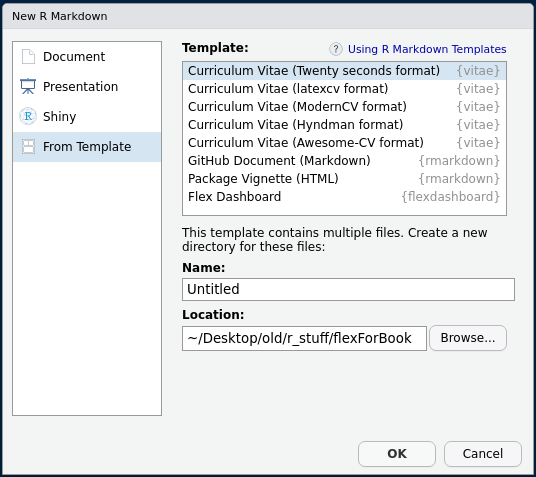
\includegraphics{flex1.png}
\caption{New session.}
\end{figure}

\hypertarget{column-based}{%
\subsection{Column based}\label{column-based}}

When we hit `OK', Rstudio give as a column based template, which is cool. Lets explore it. The flexdashboard has similar structure to the Rmarkdown. It has the same five components that the markdown has. The difference is the layout. Below, I highlighed the areas that are different. You can see two main differences: 1) Special sintax for specifying columns (or rows if the dashboard is row-based) and 2) the tripple hashes. The tripple hashes create boxes in the flexdashboard. As you might recall, in a simple markdown a tripple hash sign specifies the smallest title. Enough reading, you will understand better if you just knit this dashboard. Go agead and press `Knit'.

\begin{figure}
\centering
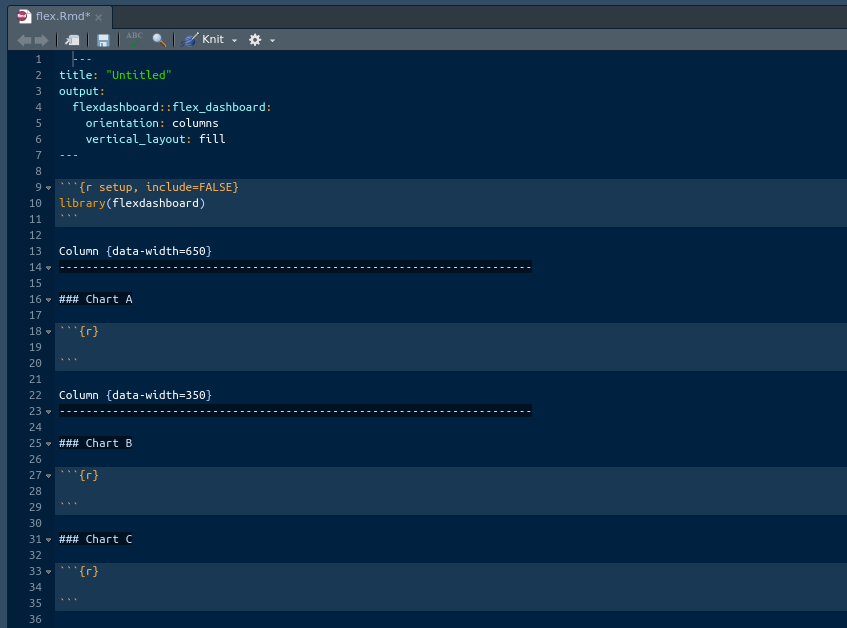
\includegraphics{flex2.png}
\caption{New session.}
\end{figure}

\begin{figure}
\centering
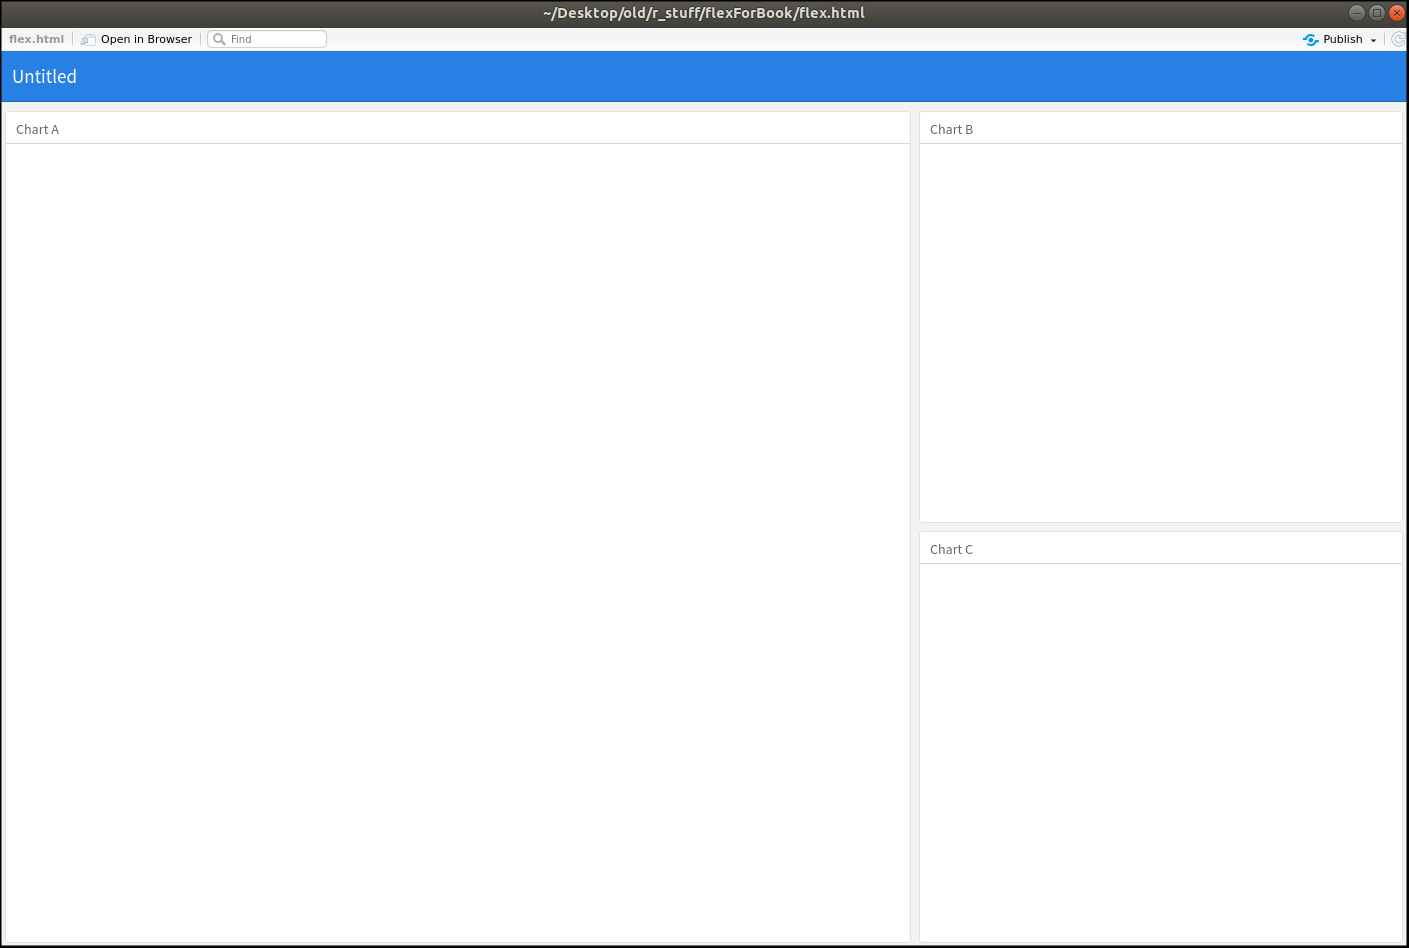
\includegraphics{flex3.png}
\caption{New session.}
\end{figure}

There you go. We got an empty dashboard. The whole layout thing should become clear now. We got the main header (blue top bar) that displays the title and three boxes that we created in the layout. As far as I know, the with of a page in R, usually, adds up to 1200px or 12, depending on the context. It does not strictly apply to the flexdahsboard for some reason. In the template, we can see that the widths of two columns add up to a thousand. Even if you the width of one of the columns to, lets say, 5000, it wont break it. Instead, it resizes proportionally. What does it mean? Means that you will have to experiment with sizes. It is not a real problem, though, so, lets move on. Lets actually insert our crash map into the main window.

Before we are able to recreate the map from the last chapter, we need to load the libraries that we will be using. They are the libraries that we have been using so far. You can just copy and paste them from our previous projects, or you can type them if you want. Use the illustration below as reference. Make sure you have all of them installed and loaded.

\begin{figure}
\centering
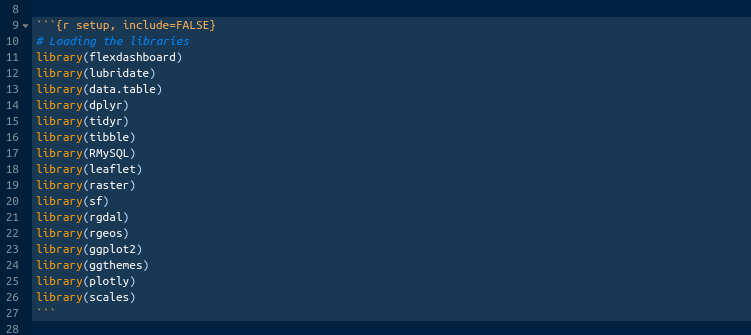
\includegraphics{flex5.png}
\caption{New session.}
\end{figure}

Now that we got the libraries down, lets prepare the data for the map. We have already done all these steps in the previous chapter, so you can just copy and paste them into the chunk. Use the illustration below as reference.

\begin{figure}
\centering
\includegraphics{flex6.png}
\caption{New session.}
\end{figure}

The data are ready. Now, literally, just copy the map code from the previous chapter and paste in the first empty chunk provided in the template under the `\#\#\# Chart A'. Use the illustration below as reference.

\begin{figure}
\centering
\includegraphics{flex7.png}
\caption{New session.}
\end{figure}

We have anough code in there to see some nice results already. Lets knit the documnet to see what it looks like at this stage. Press `Knit'.

\begin{figure}
\centering
\includegraphics{flex4.png}
\caption{New session.}
\end{figure}

This is really good already. The structure is there. The map is fully interactive. We are half way there. Lets load the second dataset. It will serve as the base for the bar plot that we will fit into the second box of the dashboard. The second one is much easier, because we do not need to agregate and join anything. When we will read it in, the date column will turn into character. We will need to revert it back to date. Reference the illustration below.

\begin{figure}
\centering
\includegraphics{flex8.png}
\caption{New session.}
\end{figure}

Once the data are in, we need to build our plot. The plot that we want to build here will be almost axactly the same as the bar plot that we built at the end of the our big assignment. Go and find that plot. It is called `ourBarPlot'. Copy it and paste into the second empty chunk provided in the template under the `\#\#\# Chart B'. There are a couple of things to change here. First, add the `fill = ``blue''\,' parameter to the geom\_bar() function. This will change the color of our bars to blue. You can pick a different color if you want. It will be dark grey if we will not include it. Second, change the title to '' (empty). We will later rename the `\#\#\# Chart B' to something else, and we do not want to have two titles there. Finally, wrap the `ourBarPlot' in the ggplotly() function to turn the ggplot2 into plotly. Reference the illustration below.

\begin{figure}
\centering
\includegraphics{flex9.png}
\caption{New session.}
\end{figure}

Once you done, knit the dashboard to see what we got.

\begin{figure}
\centering
\includegraphics{flex10.png}
\caption{New session.}
\end{figure}

We got two interactive elements that we learned in the last two chapters. Lets fill the third box. Remember I mentioned some value box and that it was important. Lets see what it is. Value boxes are great for highlighting important numbers. You can assign different colors to them and even add icons. It will be better if I just show you. Lets import the third dataset first. No modifications this time. Reference the illustration below.

\begin{figure}
\centering
\includegraphics{flex3rd.png}
\caption{New session.}
\end{figure}

Now, paste the following code in the empty chunk provided by the template under the `\#\#\# Chart C': valueBox(injuredAndKilled\$injured, icon = `fa-angry', color = `warning'). What does this mean? Well, the valueBox() is the function for value boxes. It takes the number (which is contained in the column `injured' of the table `injuredAndKilled'), icon (we are using the fontawesome icon library, here is the link for more information: \url{https://fontawesome.com/icons?d=gallery}), and color. You might wonder, what does color = `warning' mean? It is the bootstrap-library standard color. You will learn about bootsrap in the future. For now, just know that bootstrap is a styling library developed by tweeter for web developement. There are just a few standard colors in bootstrap. For instance, warning means orange.

\begin{figure}
\centering
\includegraphics{flex11.png}
\caption{New session.}
\end{figure}

Lets knit and see what we got.

\begin{figure}
\centering
\includegraphics{flex12.png}
\caption{New session.}
\end{figure}

Great. As you can see, we got an orange value box displaying the number of injuries in a big fat font with an angry face icon. Value boxes are extremely important, because they can highligh the most important numbers in your report or dashboard. Lets add the second value box displaying the number of killed. We will use red color and some different icon for it. If we just add another chunk with similar code, the value boxes will overlap for some reason. We need to add `\#\#\# Chart D' for the second value box to be properly displayed. It does not have to be `Chart D' precisely, it be called anything. We will rename them all later. Use the illustration below as reference.

\begin{figure}
\centering
\includegraphics{flex13.png}
\caption{New session.}
\end{figure}

We are almost done here. Lets knit and see what everything looks like.

\begin{figure}
\centering
\includegraphics{flex14.png}
\caption{New session.}
\end{figure}

Perfect. We are done here. One last thing to do is to change the names of the boxes from Chart A,B,C, and D to proper names. For example, instead of `\#\#\# Chart A' I wrote `\#\#\# Number of Car Accidents by Zipcode in 2019'. You can rename them as you see fit. Use the illustration below as reference for the names.

\begin{figure}
\centering
\includegraphics{flex15.png}
\caption{New session.}
\end{figure}

This is it for the row-based flexdashboard. It looks really good and is informative anough to share with others. You should have an html file with this dashboard in your project's folder. That html can be opened by most browsers and is small enough to be shared via email.

\hypertarget{row-based}{%
\subsection{Row based}\label{row-based}}

We will not have to change much to switch from the column-based layout to the row-based. Go the the hat of the document and change the orientation parameter to `rows'. See the illustration below.

\begin{figure}
\centering
\includegraphics{flex16.png}
\caption{New session.}
\end{figure}

In the body, change `Column' to Row and instead of data-width = \ldots{} write data-height = \ldots{} . You can knit the document now, but you will see that the layout is not great at all. We will have to move our bar plot from the second row to the first one. Do it according to the illustration below. Once done, knit the document to see what it looks like.

\begin{figure}
\centering
\includegraphics{flex17.png}
\caption{New session.}
\end{figure}

It is better but the value boxes are too tall. the height of the second row to 150 like below.

\begin{figure}
\centering
\includegraphics{flex18.png}
\caption{New session.}
\end{figure}

We should be go to go. Knit.

\begin{figure}
\centering
\includegraphics{flex19.png}
\caption{New session.}
\end{figure}

Good. This is usable but I prefer the column-based one.

\hypertarget{final-thoughts}{%
\section{Final Thoughts}\label{final-thoughts}}

In this section we covered everything that you need to really get started with this cool tool. There are more than just two layouts that I showed you here. However, these two are the easiest to get started with. You should use them as baselayers for your experimentations. As I said a few times here, it is much much easier to take a working prototype and start layering thing on top. You can do interesting things with flexdashboard. You can add tabs to boxes and even add multiple pages. At the moment, it should be impressive for you, but you will quickly reasize, just like I did, that flexdashboard can not do all the thing that you want. Therefore, there is no point in trying to truly master it. Instead, it makes sence to practive with it a little bit, add it to your toolbox, and move on to the topic of web applications.

This is the end of this book. I will not be teaching you anything else here. Instead, as a bonus, I want to show you a little preview of what we will be doing in the next books.

\bibliography{book.bib,packages.bib}


\end{document}
